\documentclass[conference]{IEEEtran}
\IEEEoverridecommandlockouts
\usepackage[a4paper , left=18mm, top=20mm, right=18mm, bottom=30mm, footskip=6mm]{geometry}
\setlength\parindent{0pt}
\usepackage{enumitem}
\usepackage{comment}
\usepackage[utf8]{inputenc}
\usepackage{float}
\setlength{\footnotesep}{0.4cm}
\usepackage{multicol}
\usepackage{blindtext}
\usepackage{changepage} 
\usepackage{lipsum} 
\setlength{\skip\footins}{0.5cm}
\renewcommand{\footnoterule}{%
  \kern -3pt
  \hrule width \textwidth height 0.1pt
  \kern 2.6pt
}
\usepackage{tabularx}
\usepackage {amsmath}
\usepackage{authblk}
\usepackage{tcolorbox}
\usepackage{setspace}

%\usepackage{xcolor} \pagecolor[rgb]{0.18,0.18,0.18} \color[rgb]{1,1,1}


\usepackage{hyperref}
\hypersetup{
	colorlinks=true,
    linkcolor=blue,
    filecolor=magenta,      
    urlcolor=cyan,
    pdftitle={Viral-Technical Whitepaper}
}

\usepackage{color}
\definecolor{light}{rgb}{0.5, 0.5, 0.5}
\def\light#1{{\color{light}#1}}


\usepackage{listings}
% Copyright 2017 Sergei Tikhomirov, MIT License
% https://github.com/s-tikhomirov/solidity-latex-highlighting/

\usepackage{listings, xcolor}

\definecolor{verylightgray}{rgb}{.97,.97,.97}

\lstdefinelanguage{Solidity}{
	keywords=[1]{anonymous, assembly, assert, balance, break, call, callcode, case, catch, class, constant, continue, constructor, contract, debugger, default, delegatecall, delete, do, else, emit, event, experimental, export, external, false, finally, for, function, gas, if, implements, import, in, indexed, instanceof, interface, internal, is, length, library, log0, log1, log2, log3, log4, memory, modifier, new, payable, pragma, private, protected, public, pure, push, require, return, returns, revert, selfdestruct, send, solidity, storage, struct, suicide, super, switch, then, this, throw, transfer, true, try, typeof, using, value, view, while, with, addmod, ecrecover, keccak256, mulmod, ripemd160, sha256, sha3}, % generic keywords including crypto operations
	keywordstyle=[1]\color{blue}\bfseries,
	keywords=[2]{address, bool, byte, bytes, bytes1, bytes2, bytes3, bytes4, bytes5, bytes6, bytes7, bytes8, bytes9, bytes10, bytes11, bytes12, bytes13, bytes14, bytes15, bytes16, bytes17, bytes18, bytes19, bytes20, bytes21, bytes22, bytes23, bytes24, bytes25, bytes26, bytes27, bytes28, bytes29, bytes30, bytes31, bytes32, enum, int, int8, int16, int24, int32, int40, int48, int56, int64, int72, int80, int88, int96, int104, int112, int120, int128, int136, int144, int152, int160, int168, int176, int184, int192, int200, int208, int216, int224, int232, int240, int248, int256, mapping, string, uint, uint8, uint16, uint24, uint32, uint40, uint48, uint56, uint64, uint72, uint80, uint88, uint96, uint104, uint112, uint120, uint128, uint136, uint144, uint152, uint160, uint168, uint176, uint184, uint192, uint200, uint208, uint216, uint224, uint232, uint240, uint248, uint256, var, void, ether, finney, szabo, wei, days, hours, minutes, seconds, weeks, years},	% types; money and time units
	keywordstyle=[2]\color{teal}\bfseries,
	keywords=[3]{block, blockhash, coinbase, difficulty, gaslimit, number, timestamp, msg, data, gas, sender, sig, value, now, tx, gasprice, origin},	% environment variables
	keywordstyle=[3]\color{violet}\bfseries,
	identifierstyle=\color{black},
	sensitive=false,
	comment=[l]{//},
	morecomment=[s]{/*}{*/},
	commentstyle=\color{gray}\ttfamily,
	stringstyle=\color{red}\ttfamily,
	morestring=[b]',
	morestring=[b]"
}

\lstset{
	language=Solidity,
	backgroundcolor=\color{verylightgray},
	extendedchars=true,
	basicstyle=\footnotesize\ttfamily,
	showstringspaces=false,
	showspaces=false,
	numbers=left,
	numberstyle=\footnotesize,
	numbersep=9pt,
	tabsize=2,
	breaklines=true,
	showtabs=false,
	captionpos=b
}

\usepackage{tikz}
\usetikzlibrary{shapes.geometric , arrows}
\usetikzlibrary{mindmap,trees}
\usepackage{adjustbox}
\usepackage[edges]{forest}
\usetikzlibrary{arrows.meta}

%tikzlibrary

\tikzstyle{st} = [rectangle, rounded corners, minimum width=3cm, minimum height=0.6cm, text width=3cm, text centered, draw=black, fill=red!15]
\tikzstyle{io} = [trapezium, trapezium left angle=70, trapezium right angle=110, minimum width=2cm,text width=3cm,  minimum height=0.6cm, text centered, draw=black, fill=blue!15]
\tikzstyle{pro} = [rectangle, minimum width=3cm, minimum height=0.6cm,  text centered,text width=3cm, draw=black, fill=orange!15]
\tikzstyle{dec} = [diamond, minimum width=3cm,  minimum height=0.6cm, text centered, draw=black,text width=3cm, fill=green!15]
\tikzstyle{arrow} = [thick,->,>=stealth]
\def\checkmark{\tikz\fill[scale=0.4](0,.35) -- (.25,0) -- (1,.7) -- (.25,.15) -- cycle;} 

%tikzlibrary

\usepackage{multirow}
\usepackage{tfrupee}
\usepackage{fancyhdr}
\pagestyle{fancy}
\fancyhf{} 
\renewcommand{\headrulewidth}{0pt}
\renewcommand{\footruleskip}{5mm}
\fancyfoot[C]{
\begin{center}

\includegraphics[width=0.4cm]{logo}\\
\vspace{1mm}
\thepage\\
\vspace{0.3mm}
\footnotesize{\light{viralfoundation.org}}
\end{center}
}
\usepackage{babel}
\usepackage{authblk}






\newlength{\Lnote}
\newcommand{\notte}[1]
     {\addtolength{\leftmargini}{1em}
        \settowidth{\Lnote}{\textbf{Note:~}}
        \begin{quote}
            \rule{\dimexpr\textwidth-2\leftmargini}{1pt}\\
                        \mbox{}\hspace{-\Lnote}\textbf{Note:~}%
                                            #1\\[-0.5ex] 
            \rule{\dimexpr\textwidth-2\leftmargini}{1pt}
        \end{quote}
        \addtolength{\leftmargini}{-4em}}
\graphicspath{ {./assets/images/} }


\usepackage{eso-pic}
\newcommand\AtPageUpperMyright[1]{\AtPageUpperLeft{%
 \put(\LenToUnit{0.5\paperwidth},\LenToUnit{-1cm}){%
     \parbox{0.5\textwidth}{\raggedleft\fontsize{9}{11}\selectfont #1}}%
 }}%
\newcommand{\conf}[1]{%
\AddToShipoutPictureBG*{%
\AtPageUpperMyright{#1}
}
}




%Title & Abstract Page of the Whitepaper


\title{\textbf{Viral - Next Gen Social Communication \& User Experience}}
\date{15 January 2022}
\author{Auguth Tech Pvt. Ltd.}

\setlength{\columnsep}{23pt}

\begin{document}
\singlespace
\twocolumn
%\onecolumn

\vspace{50mm}

\maketitle
\conf{January 2022}
%\onehalfspacing
\begin{abstract}

\lipsum[1]

\end{abstract}



%\tableofcontents\pagebreak 

%\twocolumn

\section{\textbf{Fad of Decentralized Social Media Apps}}

Rise of Web2 Apps\\
Rise of Privacy \& Blockchain\\
Rise of D-Apps\\
Competition with centralized\\
User Experience D-Apps offer\\
Lack of new content\\
Tiktok \& Snapchat growth vs decentralized social media at the same time frame\\
Habit forming applications\\
Transaction fee app vs free centralized apps\\
Zero Research for user experience\\
Un-ethical rewards\\
Reward for content creators only, more content more users\\
Faster content delivery\\
Why Viral won't be a fad\\
Best of decentralization\\

\section{\textbf{Vision Statement}}
To bring blockchain and crypto adoption to the masses we would got to bridge social communication with defi and tokenised economy. The Viral Network of Applications standards are designed in such a way that our vision to bring an proficient, user-friendly mobile application will combine several divisions of decentralized protocols that can lead to an ultimate tool for crypto acknowledgement. The divisions which we are focussing to rebuild is listed.\\
\\
\textbf{Social Media}
\begin{enumerate}[wide, labelwidth=!, labelindent=0pt]
\item To create a Real-world Decentralised Social Media
\item To construct an Autonomous self-evolving platform
\item To construct an Interactive Next-Gen Social Media
\item To form a clean people-owned platform appropriate for all age groups
\end{enumerate}
\textbf{Crypto Adoption}
\begin{enumerate}[wide, labelwidth=!, labelindent=0pt]
\item To provide people to hop into crypto from fiat effortlessly and securely
\item To give access to use cryptocurrencies to internet people without investing
\item To bring all major crypto for individuals to adapt rapidly using a single wallet
\end{enumerate}
\textbf{NFT and Metaverse}
\begin{enumerate}[wide, labelwidth=!, labelindent=0pt]
\item To democratize NFTs to Masses
\item To kickstart Metaverse adoption
\end{enumerate}
\textbf{Blockchain}
\begin{enumerate}[wide, labelwidth=!, labelindent=0pt]
\item To supply the utmost speed of transactions through On-Chain and Off-Chain solutions.
\item To Develop a feeless, fast, Zero Inflation, Deflationary, smart contract chain.
\end{enumerate}

\section{\textbf{Proposed Solutions}}
1. Global Multi-Tokenized Economy\\
2. Decentralized Social Media\\
3. Decentralized Immutable Storage\\
4. Avatar based- environment in social application\\
5. Met-Chat \\
6. Fully encryption algorithm and decentralized storage including public accounts\\
7. Recursive interests storing based on zk-snarks for showing better targeted posts\\
8. Highly Scalable Smart Contract blockchain on top of DAG Layer and its features\\
9. Commision based transaction fee for advanced wallets and business wallets\\
10. Transaction fee less blockchain for casual users\\
11. Deflationary Native Token with Gold-Pegged Algorithmic Stable Coin for inflation hedge\\
12. Decentralized Stable Coins for payments\\
13. Free VNS based transfers with white-listed token transfers to support multi-token economy\\
14. Viral Pay - Smart Wallet\\
15. New Swap Book based DEX\\
16. Non-Custodial Decentralized Fiat Exchange\\
17. Decentralized Bridge\\
18. Custodian Services for maximum security\\
19. Auto VSC Exchange when transfering\\
20. Viral Payment Gateway for Businesses\\
21. Decentralized Content Moderation of Social Media\\
22. Paid Open Source Initiative via Dev-Space Platform offering jobs for developers\\
23. Ad Platform connecting Influncers and clients\\
24. Decentralized Targeted Ad- Platform without tracking users data\\
25. P2P platform for anonymous fiat-crypto exchange\\
26. Global Reward System with various reward types for all contributors under the viral global system\\
27. Dividend based Viral DAO with governance features for almost all platforms except the blockchain which uses a native miners based voting system\\
28. Future plans are also explained\\

\section{\textbf{Unified Mobile Application - An Intro to Viral}}

Viral is a Next-Gen Social Media platform bridging interactive media, NFTs, and blockchain technologies' underlying applications into an every-day user-based mobile app. Viral bridges Social Media with Blockchain, Wallets, Exchanges and NFT Markeplaces to bring the ultimate one-solution for the common masses to adopt into the tokenised economy.\\

Every media shared on viral is an unique NFT where it can be utilized to create limitless achievable outcomes across the platform. Users can share ultra-short to short videos, thoughts through text, sell NFTs and additionally make communication between one-on-one, private groups and, open channels with total genuine privacy. App users will be benefited from zero ads, cryptographic encryption, censorship-resistant and, also get to use various cryptocurrencies throughout the platform. Every user is an active contributor to the platform by which they receive rewards (payment) in Viral Coin for effectively utilizing the Viral Application and it's child platforms.\\


\section{\textbf{Viral Platform Architecture}}

The Viral Platform is a fool-proof multi-platform architecture which opens up new possibilities where each platform relies on each other and supports each other's existence. The \textit{Fig.1} lists an overview about the architecture where each one are proposed vividly in further sections with it's significance and following protocols used.\\

\begin{figure*}[h]
\begin{center}
\begin{adjustbox}{width=12cm}
    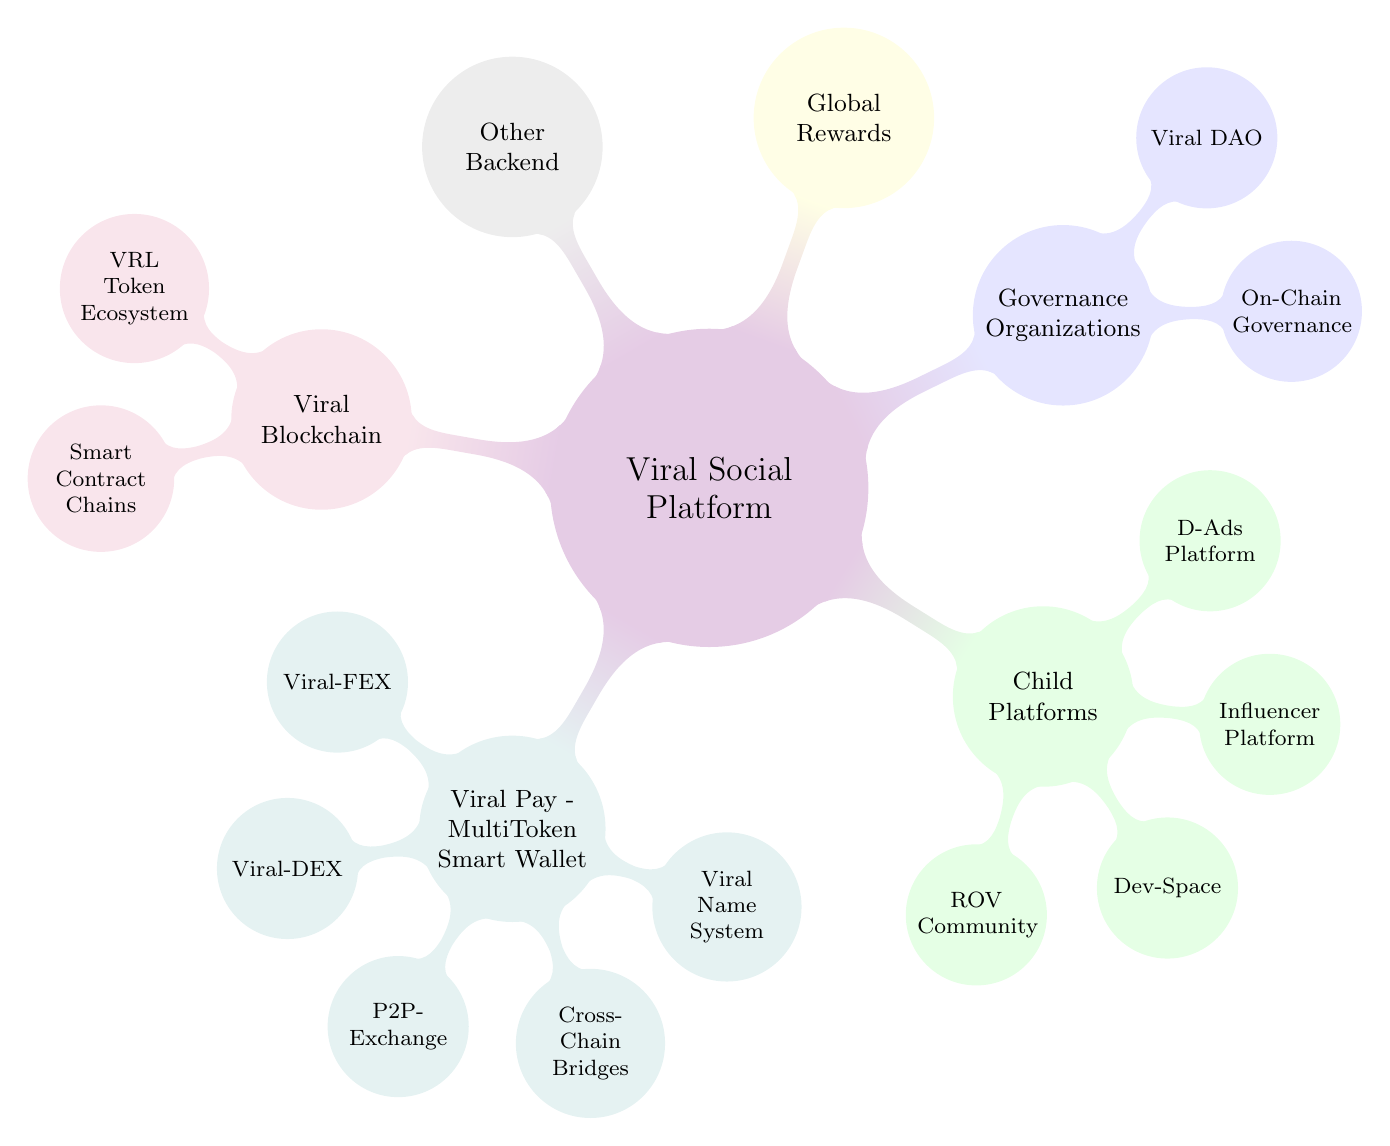
\begin{tikzpicture}
      [mindmap,
      grow cyclic,
      every node/.style=concept,
      concept color=violet!20,
      level 1/.append style={sibling angle=360/6},
      level 2/.append style={sibling angle=50},
      ]
      \node [root concept] {Viral Social Platform}
        child [concept color=purple!10, rotate=-40]{
          node    {Viral Blockchain}
          child { node    {VRL Token Ecosystem} }
          child { node    {Smart Contract Chains} }
        }
        child [concept color=teal!10, rotate=-30]{
          node     {Viral Pay - MultiToken Smart Wallet}
          child { node    {Viral-FEX} }
          child { node    {Viral-DEX} }
          child { node    {P2P-Exchange} }
          child { node    {Cross-Chain Bridges} }
          child { node    {Viral Name System} }
        }
        child [concept color=green!10, rotate=-2]{
          node  {Child Platforms}
          child { node {ROV Community} }
          child { node {Dev-Space} }
          child { node {Influencer Platform} }
          child { node {D-Ads Platform} }
        }
        child [concept color=blue!10, rotate=-4]{
          node  {Governance Organizations}
          child { node {On-Chain Governance} }
          child { node {Viral DAO} }
        }
        child [concept color=yellow!10, rotate=-20]{
          node   {Global Rewards}%[clockwise from=45, level distance=8cm]
        }
        child [concept color=black!7, rotate=-30] {
          node {Other Backend}}
        ;  
        
        \end{tikzpicture}
\end{adjustbox}
\caption{Viral Architecture}
\end{center}
\end{figure*}

\begin{enumerate}[wide, labelwidth=!, labelindent=0pt]

\item \textbf{Viral Social Platform}: Decentralized Social Media Platform bridging Blockchain applications for limitless possibilities.

\item \textbf{Viral Smart Chains}: Horizontally Scalable EVM Smart Chain on Top of IOTA's Tangle.

\begin{enumerate}[wide, labelwidth=!, labelindent=0pt]

	\item \textbf{VRL Token Ecosystem}: State Channels to move value off-chain for lightning fast micro-transactions.

	\item \textbf{Smart Contract Chains}: Sharded Horizontally scalable Smart Contract Chains anchored to Viral DAG that communicates between multiple Viral Smart Chains

\end{enumerate}

\item \textbf{Viral Pay - Multi-Token Smart Wallet}: Viral's App's built in Non-Custodial Viral Smart Chain compatible hot wallet that allows user to send and hold tokens, mint NFTs and receive rewards.

\begin{enumerate}[wide, labelwidth=!, labelindent=0pt]

\item \textbf{Viral FEX- Fiat Exchange}: Trustless Non-Custodial Exchange for Fiat-Crypto trading
\item \textbf{Viral DEX-Decentralized Exchange}: Trustless swap between multiple tokens with the new Viral Sharded DEX Protocol.

\item \textbf{P2P Exchange}: Trustsless anonymous exchange leveraging Peer-to-Peer protocol

\item \textbf{Cross-Chain Bridges}: Interopability of various major cryotocurrencies such as Bitcoin, Ethereum,etc by wrapping tokens into Viral Smart Chains.

\item \textbf{Viral Name System}: Decentralized blockchain based username protocol with token receiving preference configuration for smooth and dedicated transfers to primary wallet.

\end{enumerate}

\item \textbf{Child Platforms}: Independent platforms anchored to the viral network for effective improvement of protocols

\begin{enumerate}[wide, labelwidth=!, labelindent=0pt]

\item \textbf{Dev-Space}: Application for Developers to decide on reward allocation for improving Viral-Beta

\item \textbf{ROV Community}: Curator Platform to vote and remove reported content on Viral-Alpha
\item \textbf{Influencer Platform}: Decentralized platform connecting Influencers,businesses and users for trustless engagement-proof ads.

\item \textbf{D-Ads Platform}: Targeted Decentralized Ads without leveraging social user's data using recursive zk-snarks.

\end{enumerate}

\item \textbf{Global Rewards}: To incentivize all users, miners, developers using smart contracts for their content, validation of transactions, and continuous development through unbiased pointing strategy that offers more rewards to bigger contributors.


\item \textbf{Other Backend}: For contingencies which will be later decentralized in the further phases of the development roadmap

\end{enumerate}

\section{\textbf{Social media and User Experience}}
Viral is a multi-media sharing decentralized social network that brings meta-experience with friends, family and other people to communicate, share posts and send messages across the globe with absolute privacy. Viral sets Non-Fungible-Tokens (NFT) as a standard for every post that shared in the network which intends to bring interactive social experience and utility use cases of blockchain environment.\\

\textbf{Note} : To bring NFT as a standard for a social media post doesn't essentially implies it ought to be sold for tokens, rather it conveys that each post in Viral is a unique piece of data in the blockchain that gives the power of ownership of the user which if needed can be opted to transfer in exchange for tokens inside the Viral Platform.

\subsection{\textbf{Types of Posts}}

Posts are basically what users share to each other on their profile which will be available on the global feed comprising of all the followed and interested users posts where other users view, engage with each other to create a perfect interaction on the certain social platform. These social media posts typically consist of images, videos, texts, interactive polls, etc climbing way back to early 2000's where the advent of Friendster migrated millions of email address users to a basic online networking website, later short 1000 - 5000 word pieces known as "blogs" gained popularity among the early internet users which attracted sharing and networking with each other who shared a common goal or interest. Social Platforms what we see today such as Facebook is a product of providing better user experiences against popular platform known as MySpace which founded in 2003. By early 2006 MySpace was earth's most visited website which been overtook by Facebook in 2008 and became the prominent social media platform of the modern world acquiring various social giants which gained popularity. Media is the most important term in the social world where a social media platform thrives and registers itself as a innovative platform by means of providing better user experience by bringing exciting unique media posts.\\

A difference in other social media platforms and Viral is it's open-source nature in which the possibility of providing creative posts is not confined by the founders nor the employees of the bootstrapping organization (Viral Foundation). Centralized Social Platforms holds a pattern of posts for the users in a restricted environment which undermines the creativity of both the developers and the content creators. In some areas, centralized social platforms provide rights to developers to add different filters and AR effects to specific posts i.e., AR effects in Reels, TikToks, etc but fails to compensate the developers with it's huge ad-revenue profits and  leverages it's larger user base for open-source developers contributions. Viral aims to push the restrictions of a pattern of posts the centralized companies and decentralized social media platforms follow, and offer a multitude of creative posts (through Dev-Space Platform, explained in Developer Platform section) which will be added into the "Create" section of the Viral Social Platform where the users create various kinds of posts which will be added continuously. Currently during the social media bootstrapping stage a few post types will be available. The available posts types are given below, \\ 

\begin{enumerate}[wide, labelwidth=!, labelindent=0pt]
\item \textbf{Shots}\\

Shots are \textbf{10 sec motion pictures} with added loop transitions to bring life to photos. Pictures can be shared as shots, an exciting looped motion picture.\\
People can share their
\begin{itemize}[wide, labelwidth=!, labelindent=0pt]
\item Personal Sneak-Peek, Moments and Events
\item Exclusive Photoshoots, commercials, to your fans
\item Turn photos into lively shots by adding shot animations through Viral
\end{itemize}



\item \textbf{Thoughts}\\

Thoughts are \textbf{text-based sharing} for micro-blogging. Attach photos, long/short videos, documents, etc. There is no limit on words or media. People can share other users thoughts to their followers using re-Thought feature.\\

\item \textbf{Drops}\\

Drops are \textbf{20 second disappearing stories} shared to followers which auto-disappears once seen. It features AR filters, texts, shot elements, links, music, transitions and, much more. Every Drops will be purged in 30 days. Users will be able to view other users drops for over 30 days, once viewed will be disappeared. Drops can not be minted as unique NFT due to it's nature of disappearing media.\\

\item \textbf{Interactive Videos}\\


Interactive Videos (IV) is a short 30sec full-screen \textbf{narration based videos} which is based on interaction and \textbf{gamification of videos}.\\


\item \textbf{NFT Utilities}\\


Viral offers numerous NFT utilities within the social platform for the common users to experience the world of Non-Fungible Tokens. Minting (Creating) an NFT in Viral is\textbf{as easy as creating a social media post}. Users can buy, sell and flex their NFTs which can be previwed from the viral profile. Viral's NFTs are private, encrypted and can only be accessed by the followers. The platform will take a commission of 1.5\% per NFT sale and reverts it to the global reward pool.
\begin{enumerate}[wide, labelwidth=!, labelindent=0pt]
\item \textbf{Tunes} : Artists can \textbf{sell their music albums}, singles as NFT for the fans/people to buy and own it

\item \textbf{Sketch} : \textbf{Digital arts}, paintings, sketches can be sold through NFTs

\item \textbf{Originals} : \textbf{Physical assets} can be sold through Viral's Original NFTs where people can buy and flex

\item \textbf{Tickets} : \textbf{Exclusive passes} for events, ownership of clubs, a digital ticket for everything can be sold as NFT. 

\item \textbf{Filters} : Filters can be sold, and owned by user's thereby get rewards for it
\end{enumerate}
\end{enumerate}

\subsection{\textbf{Viral Avatars}}

Intro to Difference in Viral\\

Creating a Meta-Environment\\

What is offered\\

How Avatars are created\\

Future uses\\

Personalized Avatars are generated free for every viral user using a selfie. Users can edit their avatar skin, outfit, hair, etc. These avatars will be shown in their public profile where other users can see them 3D View. These avatars are brought into Viral to integrate metaverse and to provide an \textbf{interactive experience}\\

\begin{lstlisting}[language=Solidity]

// ReadyPlayerMe Integration Examples

1. ReadyPlayerMe WebView- How creating Avatars work using Partner API
2. Downloading Asset- GLB File using Event Listener
3. Mapping skeletons and face
4. Animating and storing the file as a 3D Viewer File inside the application using IPFS Public/Clusters
5. How Animations will work

\end{lstlisting}

\subsubsection{\textbf{Meta-Chat}}

Evolution of Chat systems\\

Integration of Live-Emotions nowdays it is all aboout experience\\

Intro to Viral Meta-Chat\\

How it works\\

Future Uses\\

Security\\

Meta-Chat is a feature to \textbf{show your facial reactions} in real-time when you chat with your friend. Viral captures your face reactions and transfer it to your avatar which the mutual friend can see on \textbf{top of his/her chat page}.

\textit{Image}\\

This gives you a \textbf{virtual experience} of videocalls through avatars and text chat.

\hyperlink{https://sample.com}{Meta-Chat Demo}\\

\textbf{SDKs and APIs Used} : List the APIs\\

\textit{Formula\\
Flowcharts}

\subsubsection{\textbf{Viral Clubs}}

Intro to Clubs\\

Evolution of Groups and Communities\\

Importance of Live community\\

Whats offered\\

How it works\\


Decentralized \textbf{Live Video Events and Audio Rooms using Avatars} (or) Normal Cams. Celebrities can host live events with their fans using their avatars\\

\textit{Image}\\
\hyperlink{https://sample.com}{Live-Events Demo}\\

\textbf{SDKs and APIs Used} : List the APIs\\

\textit{Formula\\
Flowcharts}

\subsection{\textbf{Engagements}}

\textbf{Like, Comment, Share, Tip}\\

Users can like, comment, share, reThought, and also tip Tokens to their favorite posts and influencers. The number of likes will influence the recommendations list of other users. Additionally a hidden engagement dislike will be added to every post but won't be visible to the users/nor owners, which is exclusively utilized for interest-based algorithm to filter out disliked content\\

\textbf{Tipping favorite users}\\

The tipping feature in Viral engagements tip/support user's favourite influencers' contents. It works as a donation/reward where all the tips will be directly sent to the receivers wallet. Users can send tokens of their own choice to reward other users content on the platform. Viral will charge commissions on Tips and deposits it to the global reward pool. These commissions are calculated in such a way where the percentage varies depending on the end face value. The tipping amount will be round of to tens and will leave the commision on both seperated amounts. The Charges are\\

(Ending with 1,2) tips     - \textbf{22\%}   \textit{ (i.e., 11, 62, 761, 952)}\\
(Ending with 3,4,5) tips   - \textbf{19\%}   \textit{ (i.e., 23, 64, 765, 953)}\\
(Ending with 6,7,8,9) tips - \textbf{17\%}   \textit{(i.e., 16, 48, 27,  79)}\\
(Ending with 0) tips       - \textbf{12\%}   \textit{(i.e., 10, 60, 720, 1000)}\\


For example: If a user is tips worth 57\$ then the commissions charged will be: For the first     50\$ - 12\%, remaining 7\$  - 17\%\\

\begin{figure*}
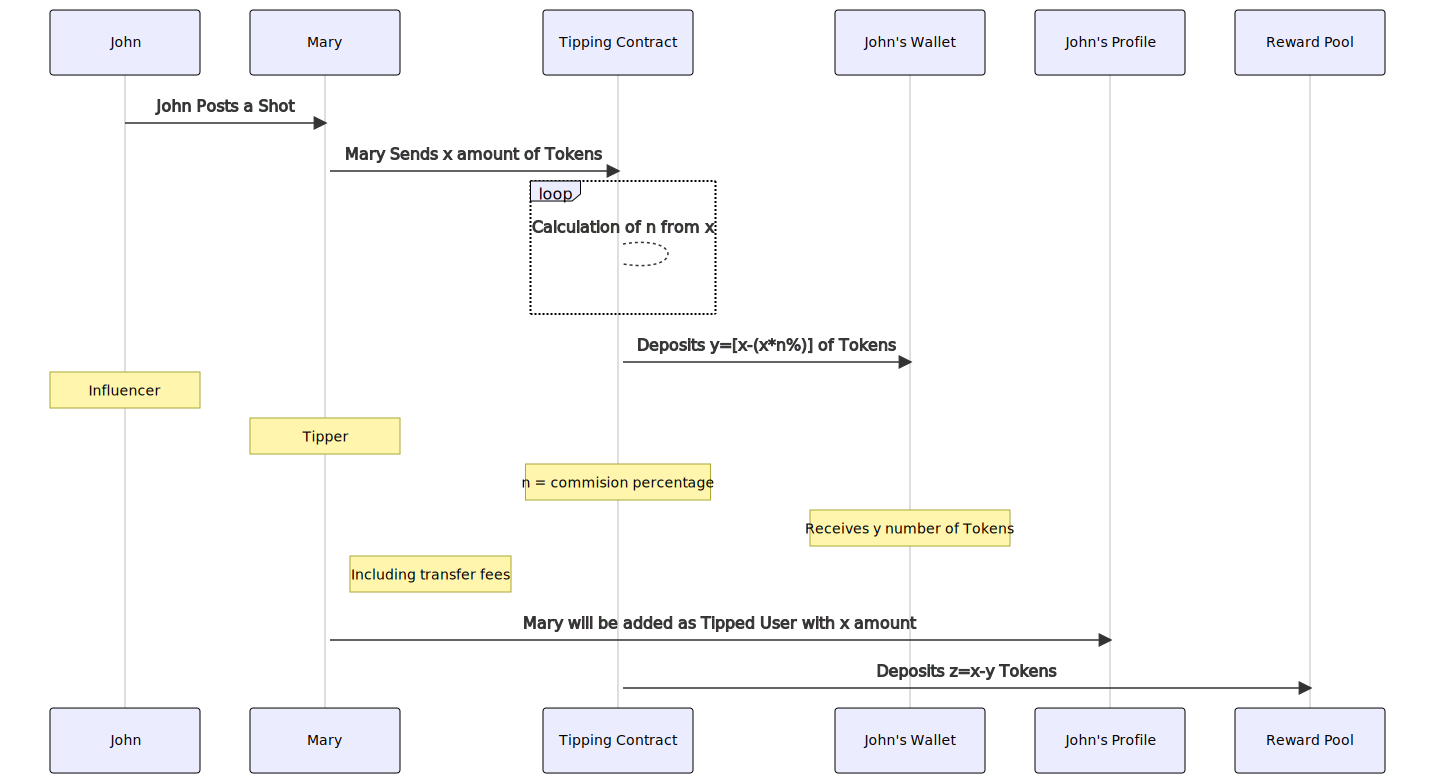
\includegraphics[width=\textwidth]{tips}\\
\caption{Tipping in Viral Social Media}
\end{figure*}

\begin{comment}%mermaid

sequenceDiagram

    participant John
    participant Mary
    participant Tipping Contract
    participant John's Wallet
    participant John's Profile
    participant Reward Pool
    

    John->>+Mary:John Posts a Shot
    Mary->>+Tipping Contract:Mary Sends x amount of Tokens
    loop 
    Tipping Contract-->Tipping Contract:Calculation of n from x
    end
    Tipping Contract->>+John's Wallet:Deposits y=[x-(x*n%)] of Tokens
    Note over John: Influencer
    Note over Mary: Tipper
    Note over Tipping Contract: n = commision percentage
    Note over John's Wallet: Receives y number of Tokens
    Note right of Mary: Including transfer fees
    Mary->>+John's Profile: Mary will be added as Tipped User with x amount
    Tipping Contract->>+Reward Pool: Deposits z=x-y Tokens

\end{comment}

\subsection{\textbf{Other Features}}

\textbf{Privacy Groups}\\

Privacy Groups is a unique feature in Viral to create unlimited friend's groups list to ensure maximum privacy for users to post and share to particular groups of users i.e., Family, Friends, Close Friends, Besties, etc. This feature can empower complete privacy over viewers for certain posts. Privacy Groups feature will benefit all the public accounts who wishes to post content specifically to their family, close friends but also maintain a public profile explicitly. Posts will only allow specific users who have read access to the content to download and decrypt the content published.  \\

\begin{figure}[H]
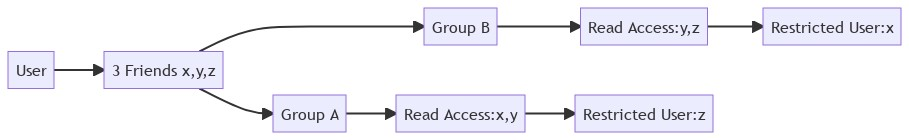
\includegraphics[width=8cm]{privacygroups}\\
\caption{Privacy Groups}
\end{figure}

\begin{comment}%mermaid
flowchart LR
    A[User]-->0
    0[3 Friends x,y,z]-->B[Group A]
    0--->C[Group B]
    B-->D[Read Access:x,y]
    C-->E[Read Access:y,z]
    D-->F[Restricted User:z]
    E-->G[Restricted User:x]
\end{comment}



\textbf{Audio Emoji}\\

This is a short feature where all the emojis in Viral if touched will give a \textbf{short sound of the emoji}. This will be accessible on chats and comments section of a post.\\

\subsection{\textbf{Viral - User Security and Privacy}}

At current world, privacy of user's in social media is being exploited by several centralized monopoly companies that run major social netwroking mobile applications that tracks user's data regarding their interests. These datas are being stored in a centralized database that is prone to attacks and breaches of private information. While targeted-manipulation plays a huge role in advertising industry, the collection of data is still prominent for almost 99\% social media business models except those run in donations. Viral focusses on maximum privacy of user's data by eliminating a central point of storage and heavily encrypts the media content circulating in the platform. It is possible to say Viral collects zero data of users and maintain a secure, trustable application in a generation where our mobiles are who we are.\\

This is classified into
\begin{enumerate}[wide, labelwidth=!, labelindent=0pt]
\item Media Storage \& Encryption
\item Chats or Private Messages
\item Interests of User
\item Chat backups
\end{enumerate}


\textbf{1. Media Storage}\\

What is IPFS\\
Benefits of IPFS\\
Other Social Apps with centralized data storage or censorless storage in IPFS with slow delivery speed\\
Viral usage of IPFS cluster\\
IPFS cluster benefits\\
Importance of CDN\\
CDNs of Different Social Media\\
Viral approach and customization of IPFS cluster\\
List of approaches and final simulation\\

Approach 1 : Viral Seira Cluster\\

Intro and Definitions\\
Abstract of the IPFS Cluster approach\\
Types of Nodes and details\\
How delivery works\\
Efficiency\\
Reward Allocation\\
Customization Parameter\\
Risks and possible problems\\

Approach 2 : Viral Monoklino Cluster\\

Abstract of the IPFS Cluster approach\\
Types of Nodes and details\\
How delivery works\\
Efficiency\\
Reward Allocation\\
Customization Parameter\\
Risks and possible problems\\

\textbf{Encryption}\\

\begin{figure}[H]
\begin{center}
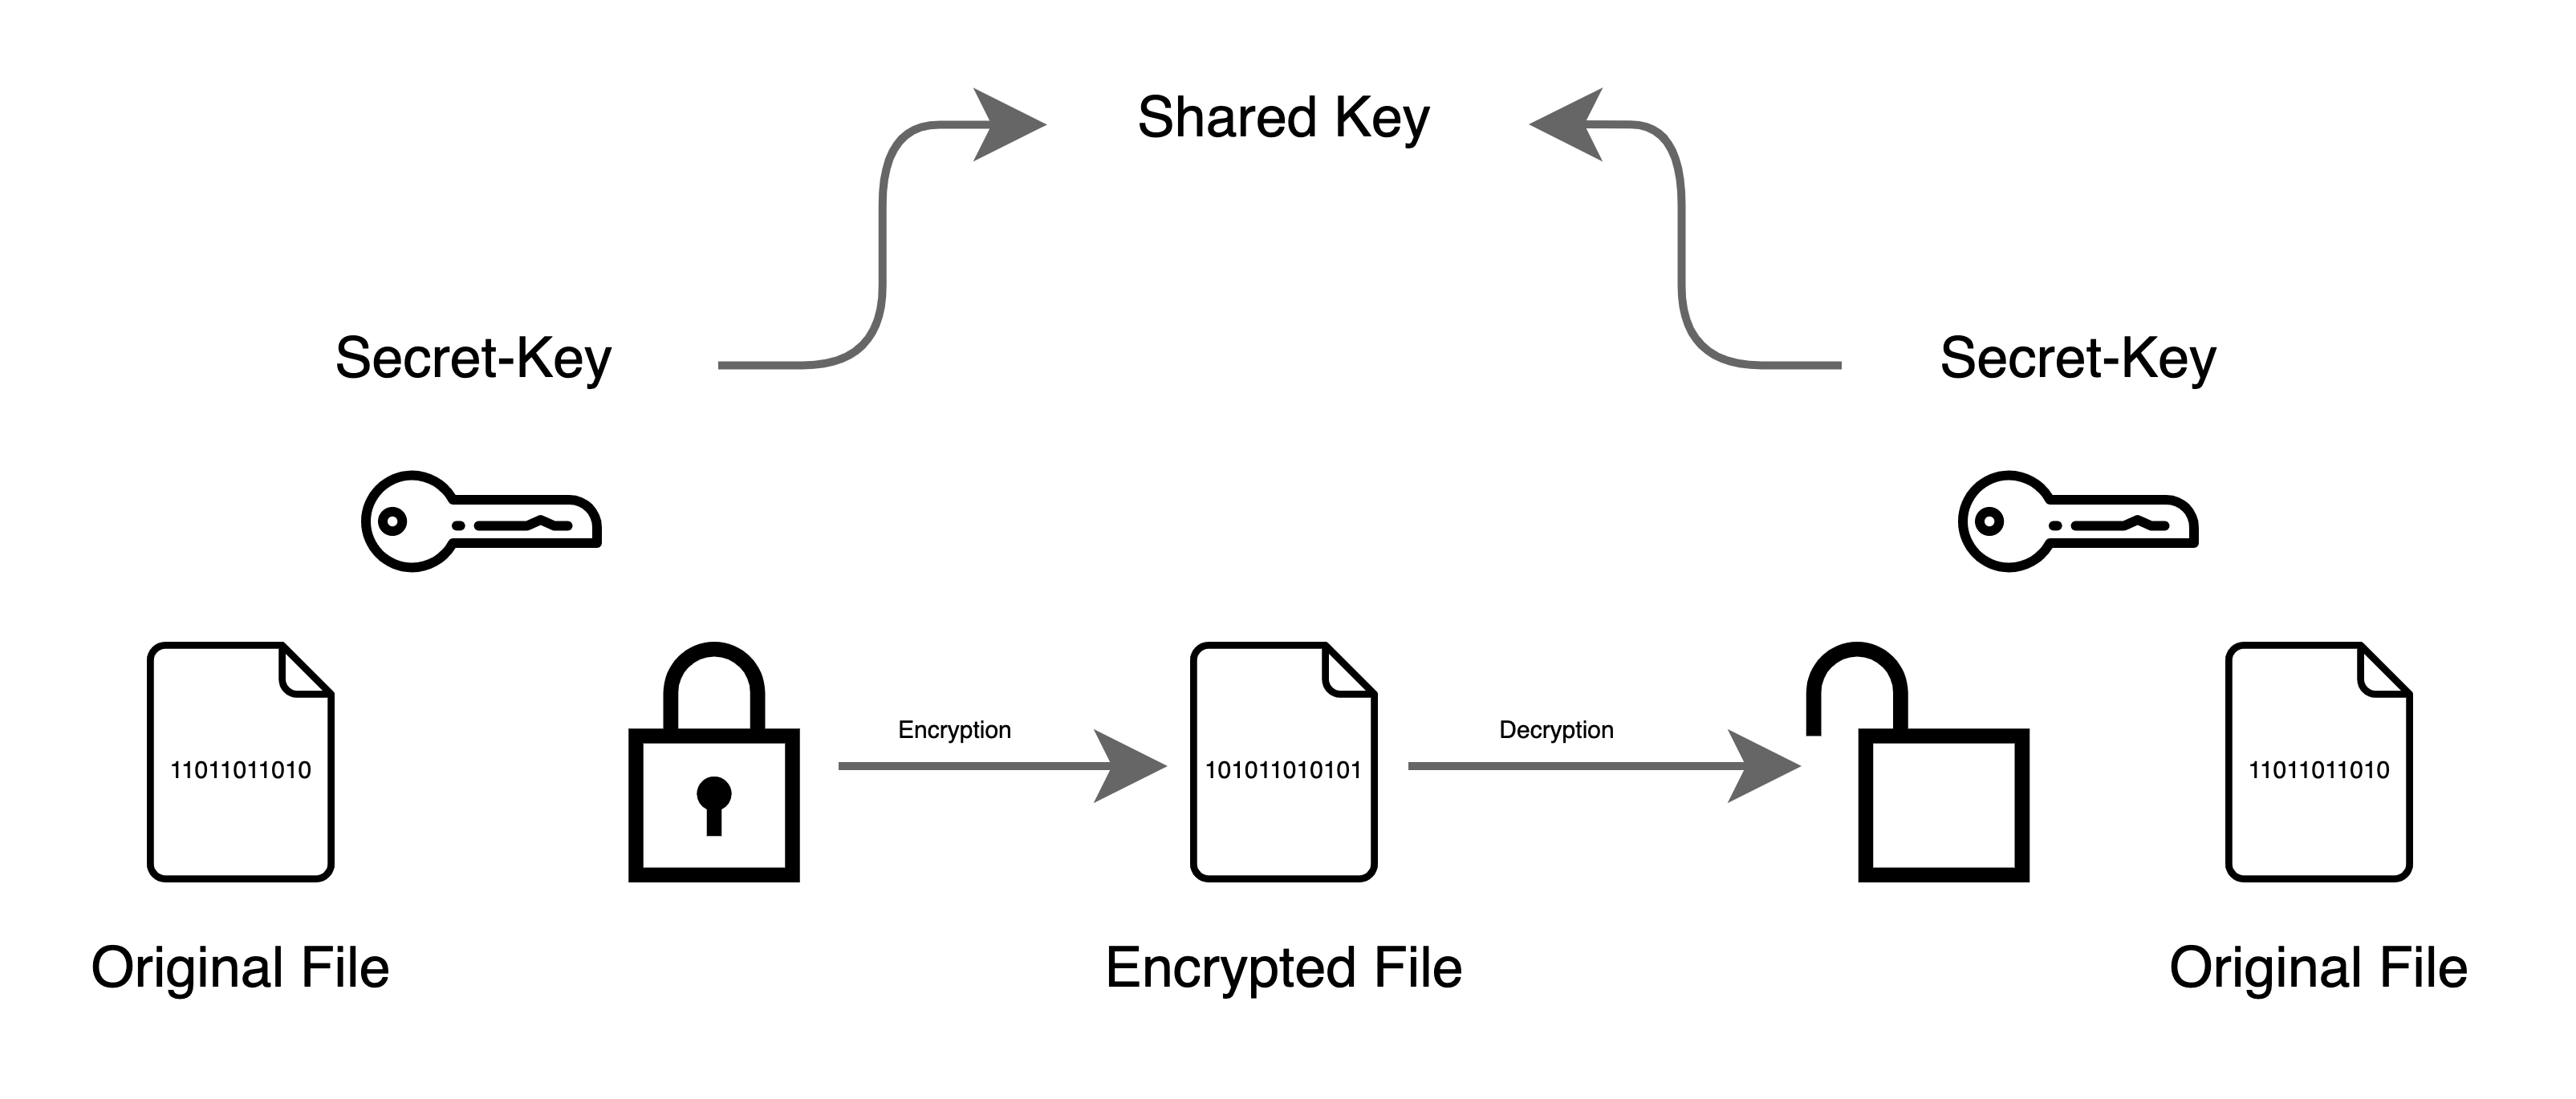
\includegraphics[width=8cm]{aes}
\caption{Symmetric Encryption}
\end{center}
\end{figure}

Viral media contents are encrypted using the Advanced Encryption Standard (AES), also known as Rijndael is a specification for the encryption of electronic data \& information established by the U.S. National Institute of Standards and Technology (NIST) in 2001. The algorithm described by AES is a symmetric-key algorithm, meaning the same key is used for both encrypting and decrypting the data. AES is the first publicly accessible cipher approved by the U.S. National Security Agency (NSA) for encrypting top secret information. AES encryption is used in our daily life mobile communications which is responsible for a large amount of security of our personal data, it is the most commonly used secure cryptographic algorithm.\\

The major reason why Viral makes use of symmetric cryptographic algorithm for securing user's data is due to the threat of quantum supremacy. If quantum computers go mainstream most encryption used in emails, secure messaging, banking services will be compromised and will be subjected to attacks. While an encryption algorithm is basically a math problem that involves a large number of bits making the most common attack (bruteforce) requiring a immeasurable amount of computing power to find the possible combinations to decipher the encrypted data, the possibilities to bruteforce are finite which puts a quantum level computing as a threat to weak encryptions that cannot be cracked by classical computers.\\

There are currently countable quantum algorithms that posses a threat to current cryptography security. Some are
\begin{enumerate}[wide, labelwidth=!, labelindent=0pt]
\item \textbf{Shor's Algorithm}\\

Originally discovered by American Mathematician Peter Shor in 1994 is a quantum computer algorithm for finding prime factors of an integer. It can target asymmetric cryptography algorithms like RSA, ECDSA, DSA, etc that uses a public-private key pair for encrypting and decrypting cipher texts. The algorithm reduces the time complexity of Integer Factorization and Discrete Logarithm from sub-exponential to polynomial, and targets keys that can have long cryptoperiods. Since, asymmetric encryption standards such as RSA heavily relies on the fact that classical computers cannot find prime factors swiftly, they are secure for now. US National Academy of Sciences, Engineering and Medicine (NASEM) predicted that a powerful quantum computer using Shor’s algorithm would be able to crack a 1024-bit encryption implementation RSA in less than 24 hours.\\

\item \textbf{Grover's Algorithm}\\

The Grover's algorithm discovered by Lev Grover, could theoretically weaken the security of symmetric cryptographic algorithms, such as Advanced Encryption Standard (AES). Grover's algorithm could brute-force a 128-bit symmetric cryptographic key in roughly 2$^{64}$ iterations, or a 256-bit key in roughly 2$^{128}$ iterations. As a result, it is sometimes suggested that symmetric key lengths be doubled to protect against future quantum attacks.  In short, Grover's algorithm reduces the brute-force attack time to it's square root, so the attack time for a 128bit AES encryption is decreased to 2$^{64}$, where the 256bit encryption is reduced to 2$^{128}$ which is considered secure.\\

Since AES-256 is proven to be the best well-used algorithm currently during post-quantum era, Viral encrypts all the user data using 256bit key symmetric encryption. \\
\end{enumerate}

\textbf{Encryption}\\

The steps for Encryption, Media Uploading, IPFS Pinning, Cluster Repetition, Post-Meta-Data Update are given as following
\begin{itemize}[wide, labelwidth=!, labelindent=0pt]
\item After the media is done for preparation it will begin the encryption process by generating a 256-bit random key.
\item The encryption is done locally inside the device and the encrypted file is generated
\item The encrypted file later hosted to a server that takes the file and pins it to a series of IPFS Public nodes
\item After it is hosted to the Public Nodes via a common IPFS-CID (content-identifier) that CID is pinned on to the IPFS Private Clusters which tracks pins across a cluster of IPFS daemons and uses a leader-based consensus algorithm Raft to coordinate storage of a pinset, distributing the set of data across the participating private nodes.
\item The file is pinned on both Public and Private CLuster Nodes
\item The Repetition of Files among the cluster nodes are determined and configured previously. In summary, the file will be repetitively stored across IPFS-Private-Cluster Nodes. The repetition is monitored by configuring a minimum and a maximum repetition level.
\item After pinning to a single IPFS-Private-CLuster the CID is updated in the post meta-data along with the secret-key which is generated while encrypting the media content
\item The Content is stored in a decentralized, secure and encrypted manner where neither an exploiter nor the developers on Viral can able to view user's content inside publicly available IPFS nodes.
\end{itemize}

\begin{figure}[H]
\begin{center}
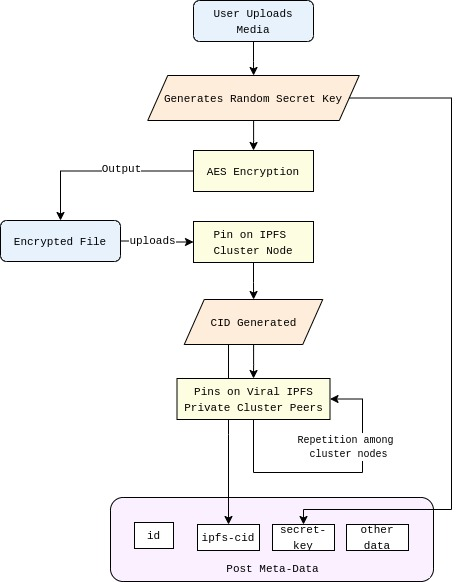
\includegraphics[width=7cm]{encryption}
\caption{Encryption of Media in Viral}
\end{center}
\end{figure}

\begin{lstlisting}[caption={Post Meta-Data}, numbers=none]

	post id:12 {
    	"cid": "hefTFbifw5P4gXftAwvA4eXQ89f9w7RA...",
    "caption": "This is a sample caption",
    	"gateway": "https://cluster.viral.com/",
    	"secret-key" : "PdSgVkYp3s6v9y$B?E(H+MbQ..."
	}
\end{lstlisting}

\textbf{Decryption}\\

Decryption is classified into two categories
\begin{enumerate}[wide, labelwidth=!, labelindent=0pt]
\item \textbf{Private Account Media Decryption} : Decrypting Private Media which can be only accessed by white-listed user approved followers with maximum privacy and security
\item \textbf{Public Account Media Decryption} : Decrypting Public Media which can be accessed by anyone instantly by openly allowing users to fetch the secret keys.
\end{enumerate}

\textbf{Private Account Media Decryption}\\

\begin{figure}[H]
\begin{center}
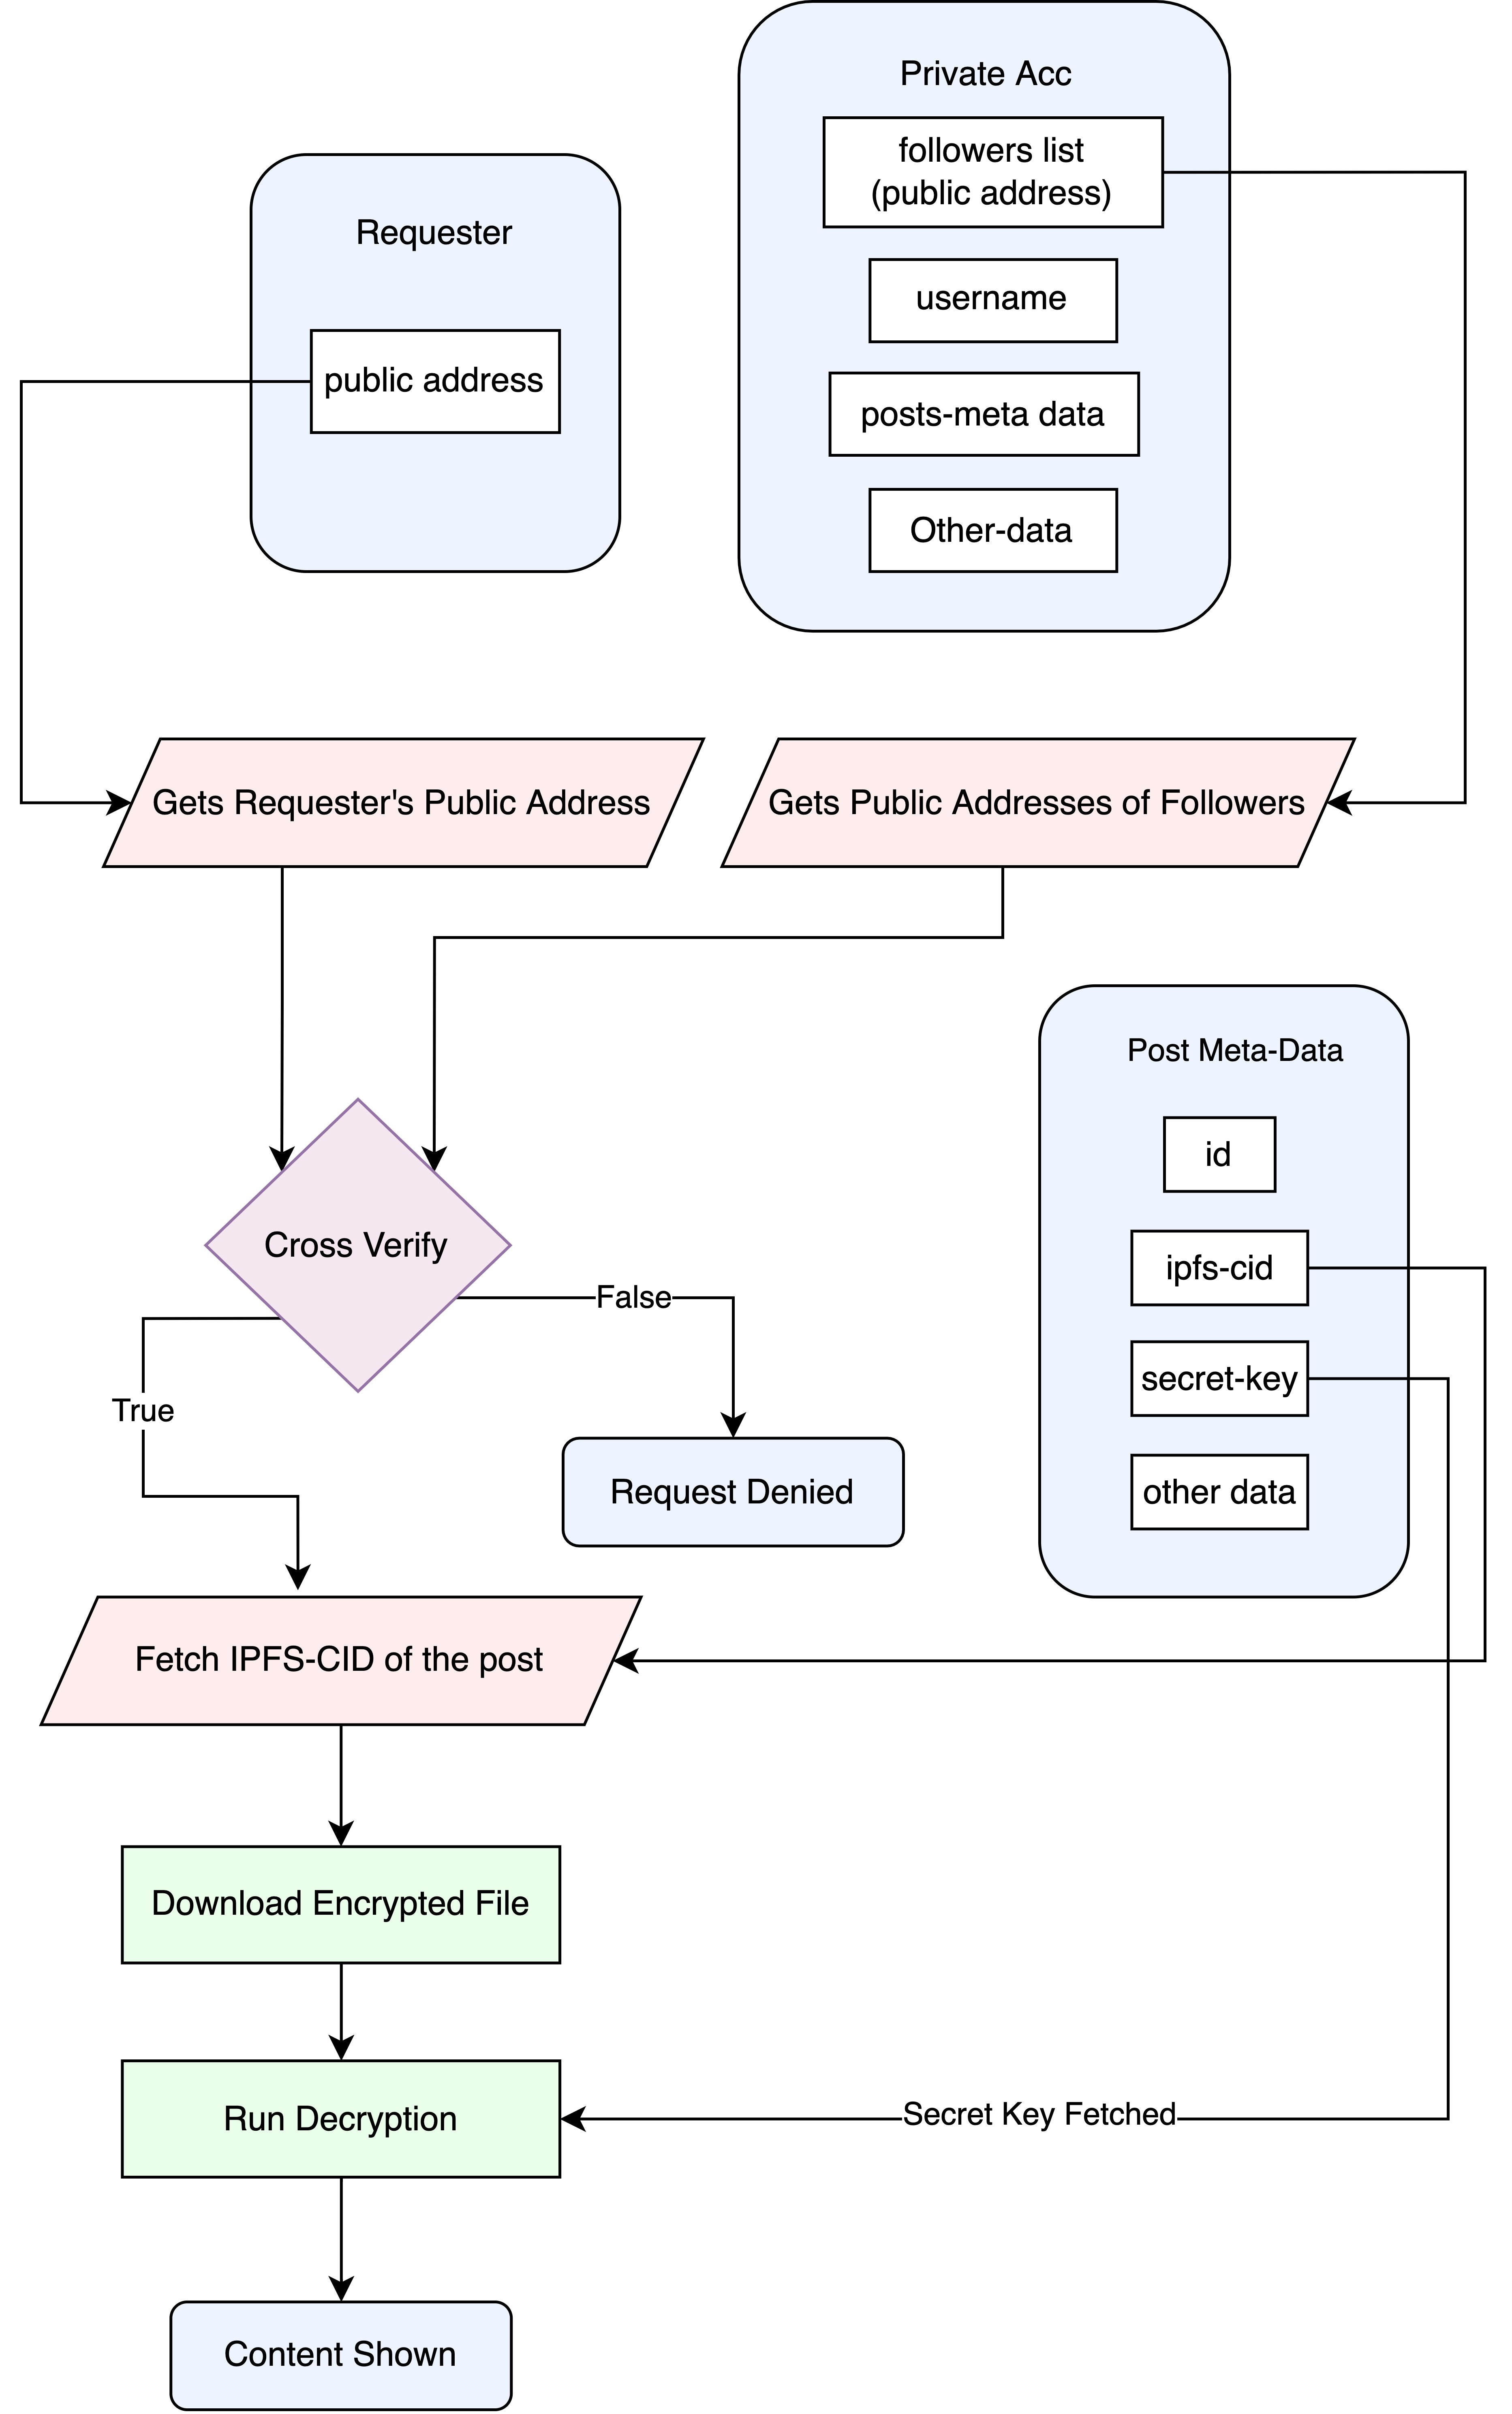
\includegraphics[width=6cm]{decryption-private}
\caption{Decrypting Media of Private account in Viral}
\end{center}
\end{figure}

The Steps on Fetching Public Addresses of content view requester, verification, fetching IPFS CID, downloading and decrypting content is specified below
\begin{itemize}[wide, labelwidth=!, labelindent=0pt]
\item A Private Account will be limiting it's content access to certain white-listed users that is been approved/accepted by the admin user. Every Viral account shall have a public address which will be added to the white-listed users list.
\item The Public address of the Requester shall be fetched and cross verified with the white-listed user list of the private account. Only the white=listed user will be able to unlock the private account.
\item The meta data of the posts will be decrypted to the white-listed user and the user shall fetch the IPFS-CID and the secret-key of the encrypted file
\item The file is downloaded and decrypted using the symmetric secret-key and the content is shown
\end{itemize}


\textbf{Public Account Media Decryption}\\

\begin{figure}[H]
\begin{center}
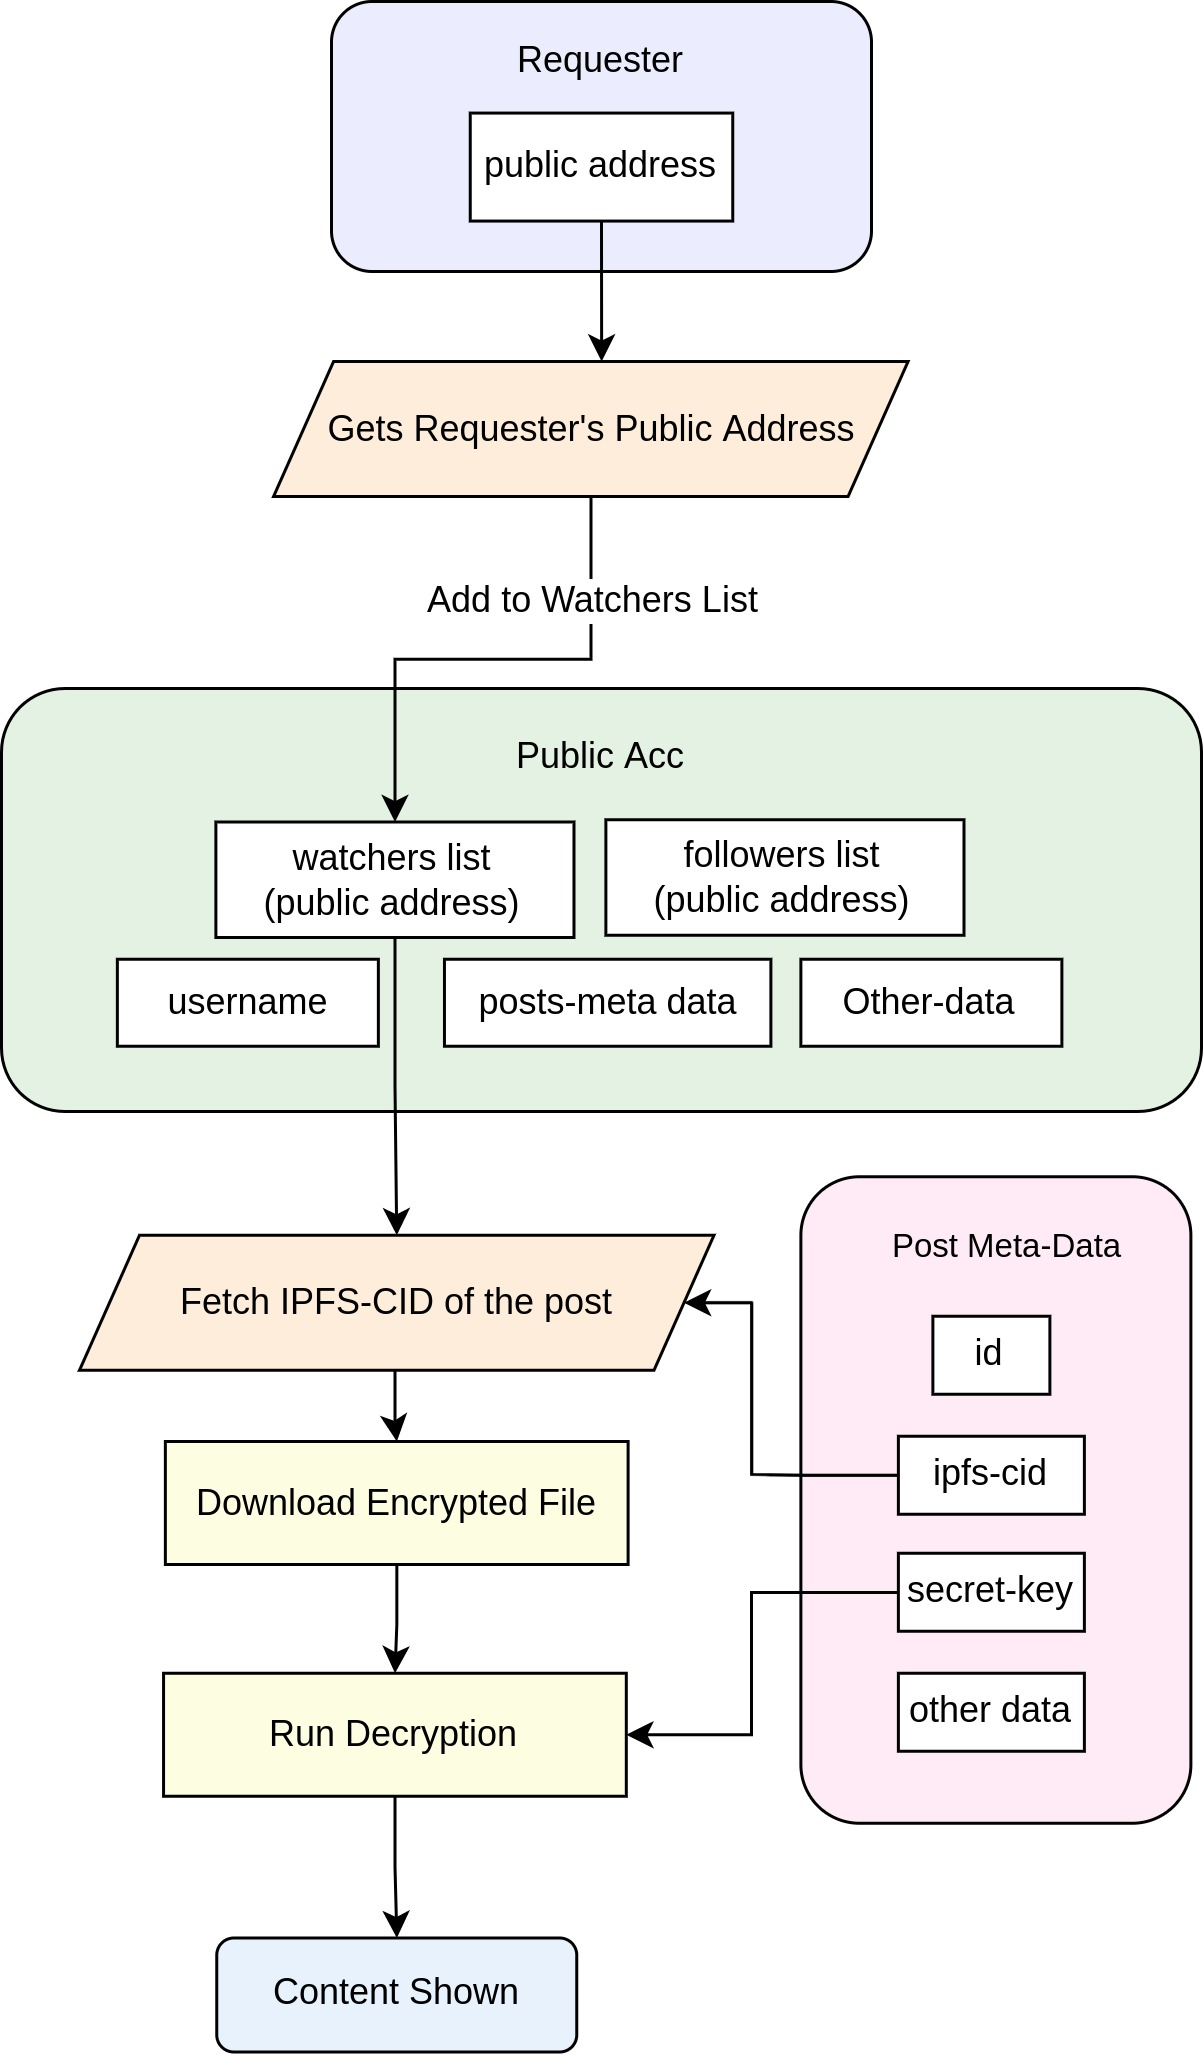
\includegraphics[width=6cm]{decryption-public}
\caption{Decryption Media of Public account in Viral}
\end{center}
\end{figure}

Viral ensures that all the content in the social application is securely encrypted compared to current poorly encrypted social media platforms that takes a stealthy look on to people's content even if the account is configured as private. While Public accounts are not encrypted, the storage of files is done centralized on the entity's server farms. Viral is a decentralized social media service that allows anyone to contribute as a storage node and receive rewards in return for the contribution towards the network. This positively puts a violation of storing individual/organizations data which can be used for multiple exploitation attempts due to the growing adoption on big data, machine learning, artificial intelligence, etc.  Neverhtless Viral needs to encrypt public accounts data/content in the most secure manner for nodes to collectively host as a decentralized open network and also providing trust and security to users data. The process of decrypting a public account post is done by maintaining a real-time white-list of users public addresses called "Watchers-list". Viewer's public addresses shall be added in the watchers list to fetch the cid and the secret-key from posts that can decrypt the downloaded content. This way we can ensure the exact security we have in private accounts in public accounts as well.\\


\textbf{2. Chats and Private Messages}\\

For Chat-based encryption, Viral uses \textbf{public and private key} encryption method. Viral Chat is an Offline-First chat messenger which doesn't comprises of centralized cloud-based servers involved in storing messages which can potentially trigger breaches. Every single message is encrypted and can be only decrypted by the receiver.\\

\begin{figure}[H]
\begin{center}
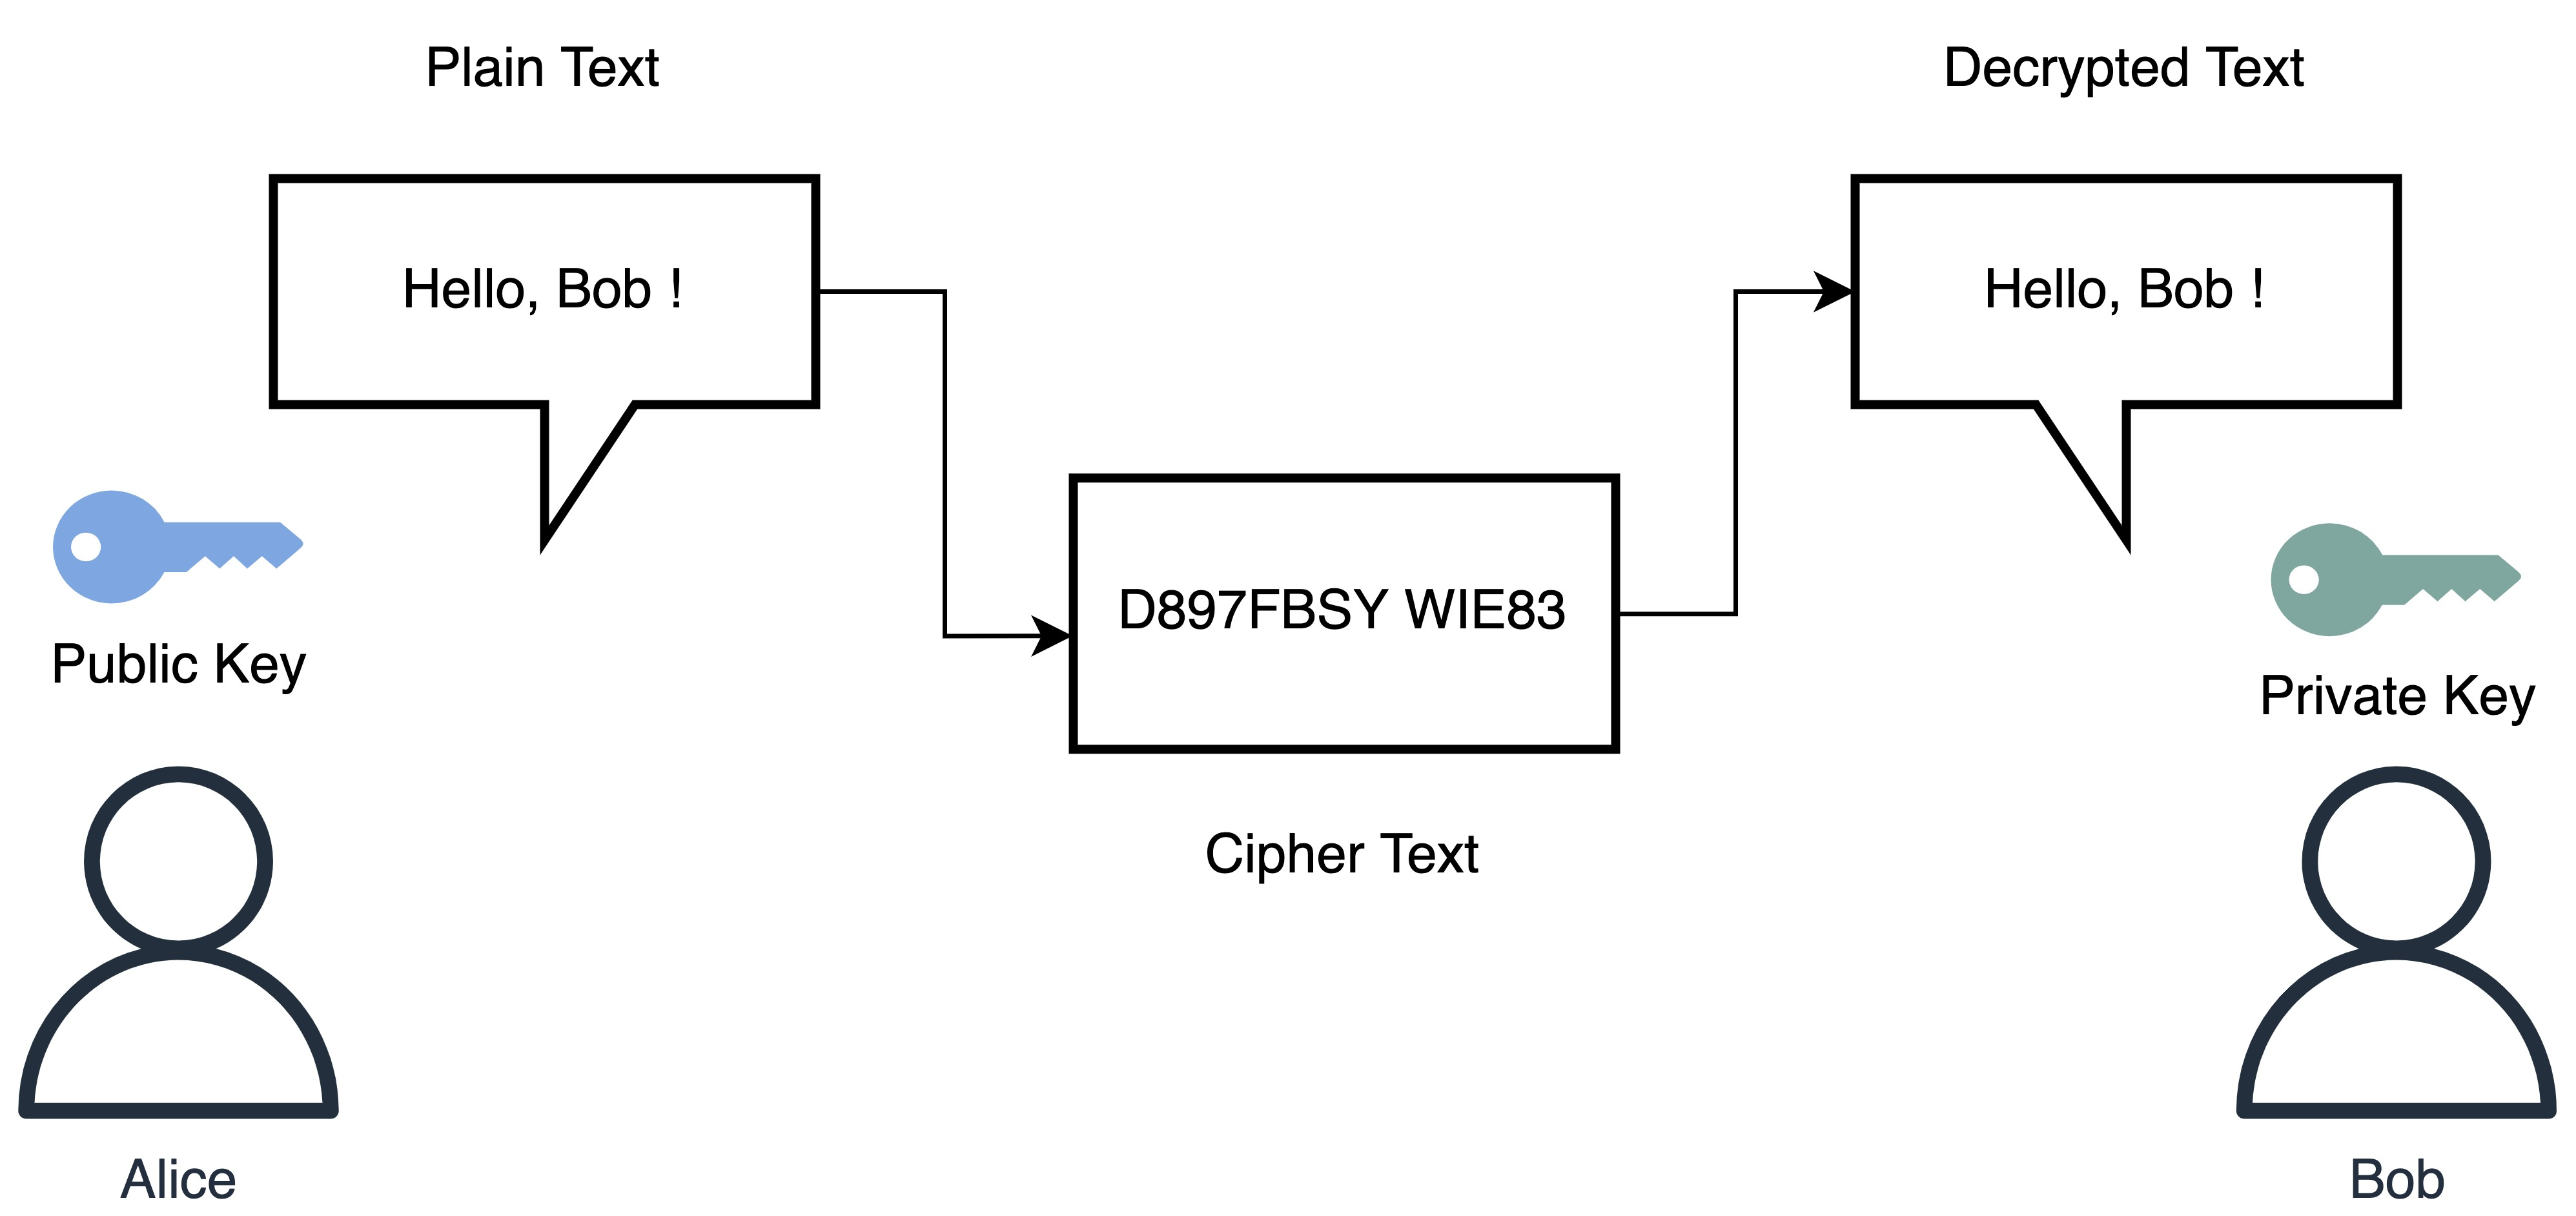
\includegraphics[width=7cm]{chat}
\caption{Asymmetric Chat Encryption}
\end{center}
\end{figure}

\textbf{3. Interests of User}\\


To make the viral platform more user-friendly interest-based recommendations are utilized. We have numerous ways to fetch interest from a user \textbf{without collecting data on a centralized server}, a few of them are
\begin{itemize}[wide, labelwidth=!, labelindent=0pt]
\item Like and Dislike
\item Hashtag Follows
\item Search-Based Interests
\item Based on Activity
\item Shares with other friends
\item Following interests
\item Based on Comments
\end{itemize}

All the user interests will be \textbf{stored locally} on the device to ensure \textbf{maximum security} and will be taken to show recommendations. Users' interests will be \textbf{saved locally} on their devices ensuring full privacy of personal data.\\

\textbf{4. Chat Backup}\\

Since Viral is a \textbf{Offline-First Chat} messages will not be stored in cloud. To Backup messages Viral will offer \textbf{cloud options} such as Google Drive/Dropbox where you can securely encrypt and save your \textbf{backup}. The encryption will be based on AES Standard and will be only decrypted upon providing the password key on request. ALl the Data including messages and interests are backed-up and restored when required .\\

\textbf{Phase 2 Development}\\

We will be focussing on Quantum Resilience of all media encryption used in Viral while commencing the Phase 2 of Development Roadmap\\

\subsection{\textbf{TOR/VPN Anonymity}}

Viral will be a safe haven for anonymity, privacy, and security in eliminating the tracing of users' identities by exploiters . Users can benefit from TOR and VPN Routing Features built in our Decentralized application to hide their IP address and go fully anonymous.\\

TOR routes you through several additional nodes while encrypted, no one can trace it back to you. VPN will redirect your internet traffic through a secure tunnel, hiding your IP address and encrypting your data in the process.\\

\section{\textbf{Blockchain, Token Ecosystem}}

Abstract of Viral Smart Chains\\
Introduction\\
Adoption statistics of current blockchains\\
People statistics report of blockchain adoption\\
Why current blockchains doesn't get major adoption\\
What stops people from using blockchain as financial tool\\
People Category and Idealogies\\
Usefullness of blockchain\\
How future will look if a billion people use blockchain\\
Governmental pressure and need for regulation\\
Explicit and shadow banning effects among investors\\
Misinterpretation of blockchain for laundering money\\
Ideal blockchain for the world\\
Benefits of both decentralized and centralized worlds\\
Features needed for a widespread option\\
Need for a universal bridge for connecting blockchains to governments for financial revolution\\

\subsection{\textbf{Viral Smart Chain – Short Intro}}

Viral Smart Chains, is a network of parallel Smart Contract Chains on top of a altered Tangle (IOTA) used for Viral Social network with fully deployed defi ecosystem. Viral Smart Chains aim to provide an easy understandable one-platform for all the non-crypto users who are subjected to higher gas fees, congestion in network, volatility and scattered defi solutions. \\

\subsection{\textbf{Tangle}}

The Tangle (by IOTA Foundation) is a next generation Distibuted Ledger Technology that utilizes a new data structure based on Directed Acyclic Graph. Tangle by contrast, does not consist of transactions grouped into blocks and stored in sequential chains, but as a stream of individual transactions entangled together. To do transactions in the network a participant should need to carry out a small computation work to verify two previous transaction. This makes tangle a linearly scalable ledger by network activity implementing participants/users as miners. Transactions in Tangle are completely feeless where miner incentives/rewards are eliminated by providing validation for their own transaction. Instant confirmations and transaction finality is achieved within seconds with low computation requirements.

\subsection{\textbf{IOTA Smart Contract Protocol}}

IOTA provides an Off-Chain Smart Contract Solution for developers to create multiple-chains on Top of Tangle. Since Ethereum transactions are processed On-chain by every single node on its network, it faces additional congestion, slow transaction time and subject to higher miner fees. IOTA's off-chain smart contract solution makes use of blockchains anchored to the Tangle where the smart contracts are ran and achieved consensus with small set of committee nodes. This achieves a high scalable throughput and immutable records since the states of smart contracts such as Account Balances, Input Conditions and Consequences over time are updated on the Tangle. There are several components to understand more about IOTA's Smart Contracts Protocol. It gives us multi-chain functionality to run smart contracts from different chains which allows a horizontal scaling of blockchains without a need for plasma or side chains.\\

\textbf{Consensus and Validators}\\

IOTA's Smart Contract Chain uses a Byzantine Fault Tolerant \(BFT\) Algorithm, which guarantees consistency and byzantine fault tolerance if less than $1/3$ of nodes are malicious. So the verification process runs on Nodes within a chain committee.The validators of the chain \(Nodes\) form a committee, a bound together closed set of nodes. The committee of the chain can allow new validators and validator nodes to be added or replaced. This also makes the chain itself agnostic to its validators \(the committee\).\\

Only when a supermajority of the validators (the quorum) of a chain reaches consensus, the results get added to the chain where a new state update can be signed, which unlocks the AliasOutput for the chain and produces the next state UTXO which is stored on the Tangle as an immutable record. In summary, the chain's state (data) will be stored on Tangle as an immutable record.The amount of the validators to reach a consensus is configurable for each chain. The committee itself can also be variable in size - from a few nodes up to hundreds of nodes, and each node can be part of many different committees.\\

\begin{itemize}[wide, labelwidth=!, labelindent=0pt]
\item \textbf{Validators} – Each Single Node running the Chain
\item \textbf{Committee} – The Group of Nodes running a chain
\item \textbf{Quorum} – Number of Nodes to be in consensus to validate a transaction
\end{itemize}

To know more about IOTA's Smart Contracts : \hyperlink{https://files.iota.org/papers/ISC_WP_Nov_10_2021.pdf}{Whitepaper}, \hyperlink{https://wiki.iota.org/smart-contracts/overview}{Documentation}, \hyperlink{https://blog.iota.org/iota-smart-contracts-beta-release/}{Blogs}\\

\subsection{\textbf{Viral \& IOTA}}

While Tangle with Multi-chain functionality is the future of decentralized applications and scalable contract executions, there is still room for improvements because of developers facing a multitude of disagreements inside the protocol which also applies for running a user-focussed application like Viral. \\

\textbf{Dust Protection}\\

The huge disagreement of the various IOTA Protocols is the Dust protection scheme that requires every wallet to have a returnable deposit of Tangle's native asset IOTA in order to successfully transfer various tokens both fungible and non-fungible. In simple terms if a user would want to hold a Non-Fungible-Token in his/her wallet, the user should have a deposit of a certain IOTA coins. This dust protection scheme is introduced to avoid bloating the distributed ledger's size due to fee-less micro-transactions. By eliminating fees the utility for the native asset will decrease if various tokens are being constantly deployed. Viral users are aimed to be common social media users who may not able to deposit a certain IOTA to mint NFTs, send Viral Coins (assuming it's on Tangle) to their friends and family. The Dust protection scheme of the new tokenization framework avoids the usage of IOTA Foundation's Smart Contract Protocol due to Viral's fundamental vision of dissolving preplexing rules of using a crypto wallet and democratize into a simple solution in blockchain applications that feel the same as current simple web 2.0 applications.

\subsection{\textbf{Viral - Side Tangle}}

During disagreements and inability to change the native protocol due to lack of votes, developers fork native block-chains to run a separate block-chain with added functionality that dissolves the disagreement by bringing required changes to the forked(new) protocol. While forked block-chains takes a snapshot of user's balances until a certain block number in the native protocol to convert current coins into newly forked coins that's circulated. Some forks doesn't take snapshots but only forks the source-code to bring necessary changes to the protocol and run independently starting from the genesis block. Since dust-protection scheme of the tokenization framework is a huge concern for a seamless usage of the Viral Application, a source-code fork of the Tangle and the ISC is intend to happen with added functionalities that tie up with the vision of a non-complex crypto solution for the common people and a better framework for existing problems that IOTA encounters such as dust protection, increasing ledger size, decentralization and security of user's funds on less secure chains on top of Tangle.











\subsection{\textbf{Viral Smart Chains}}

\begin{figure*}
\begin{center}
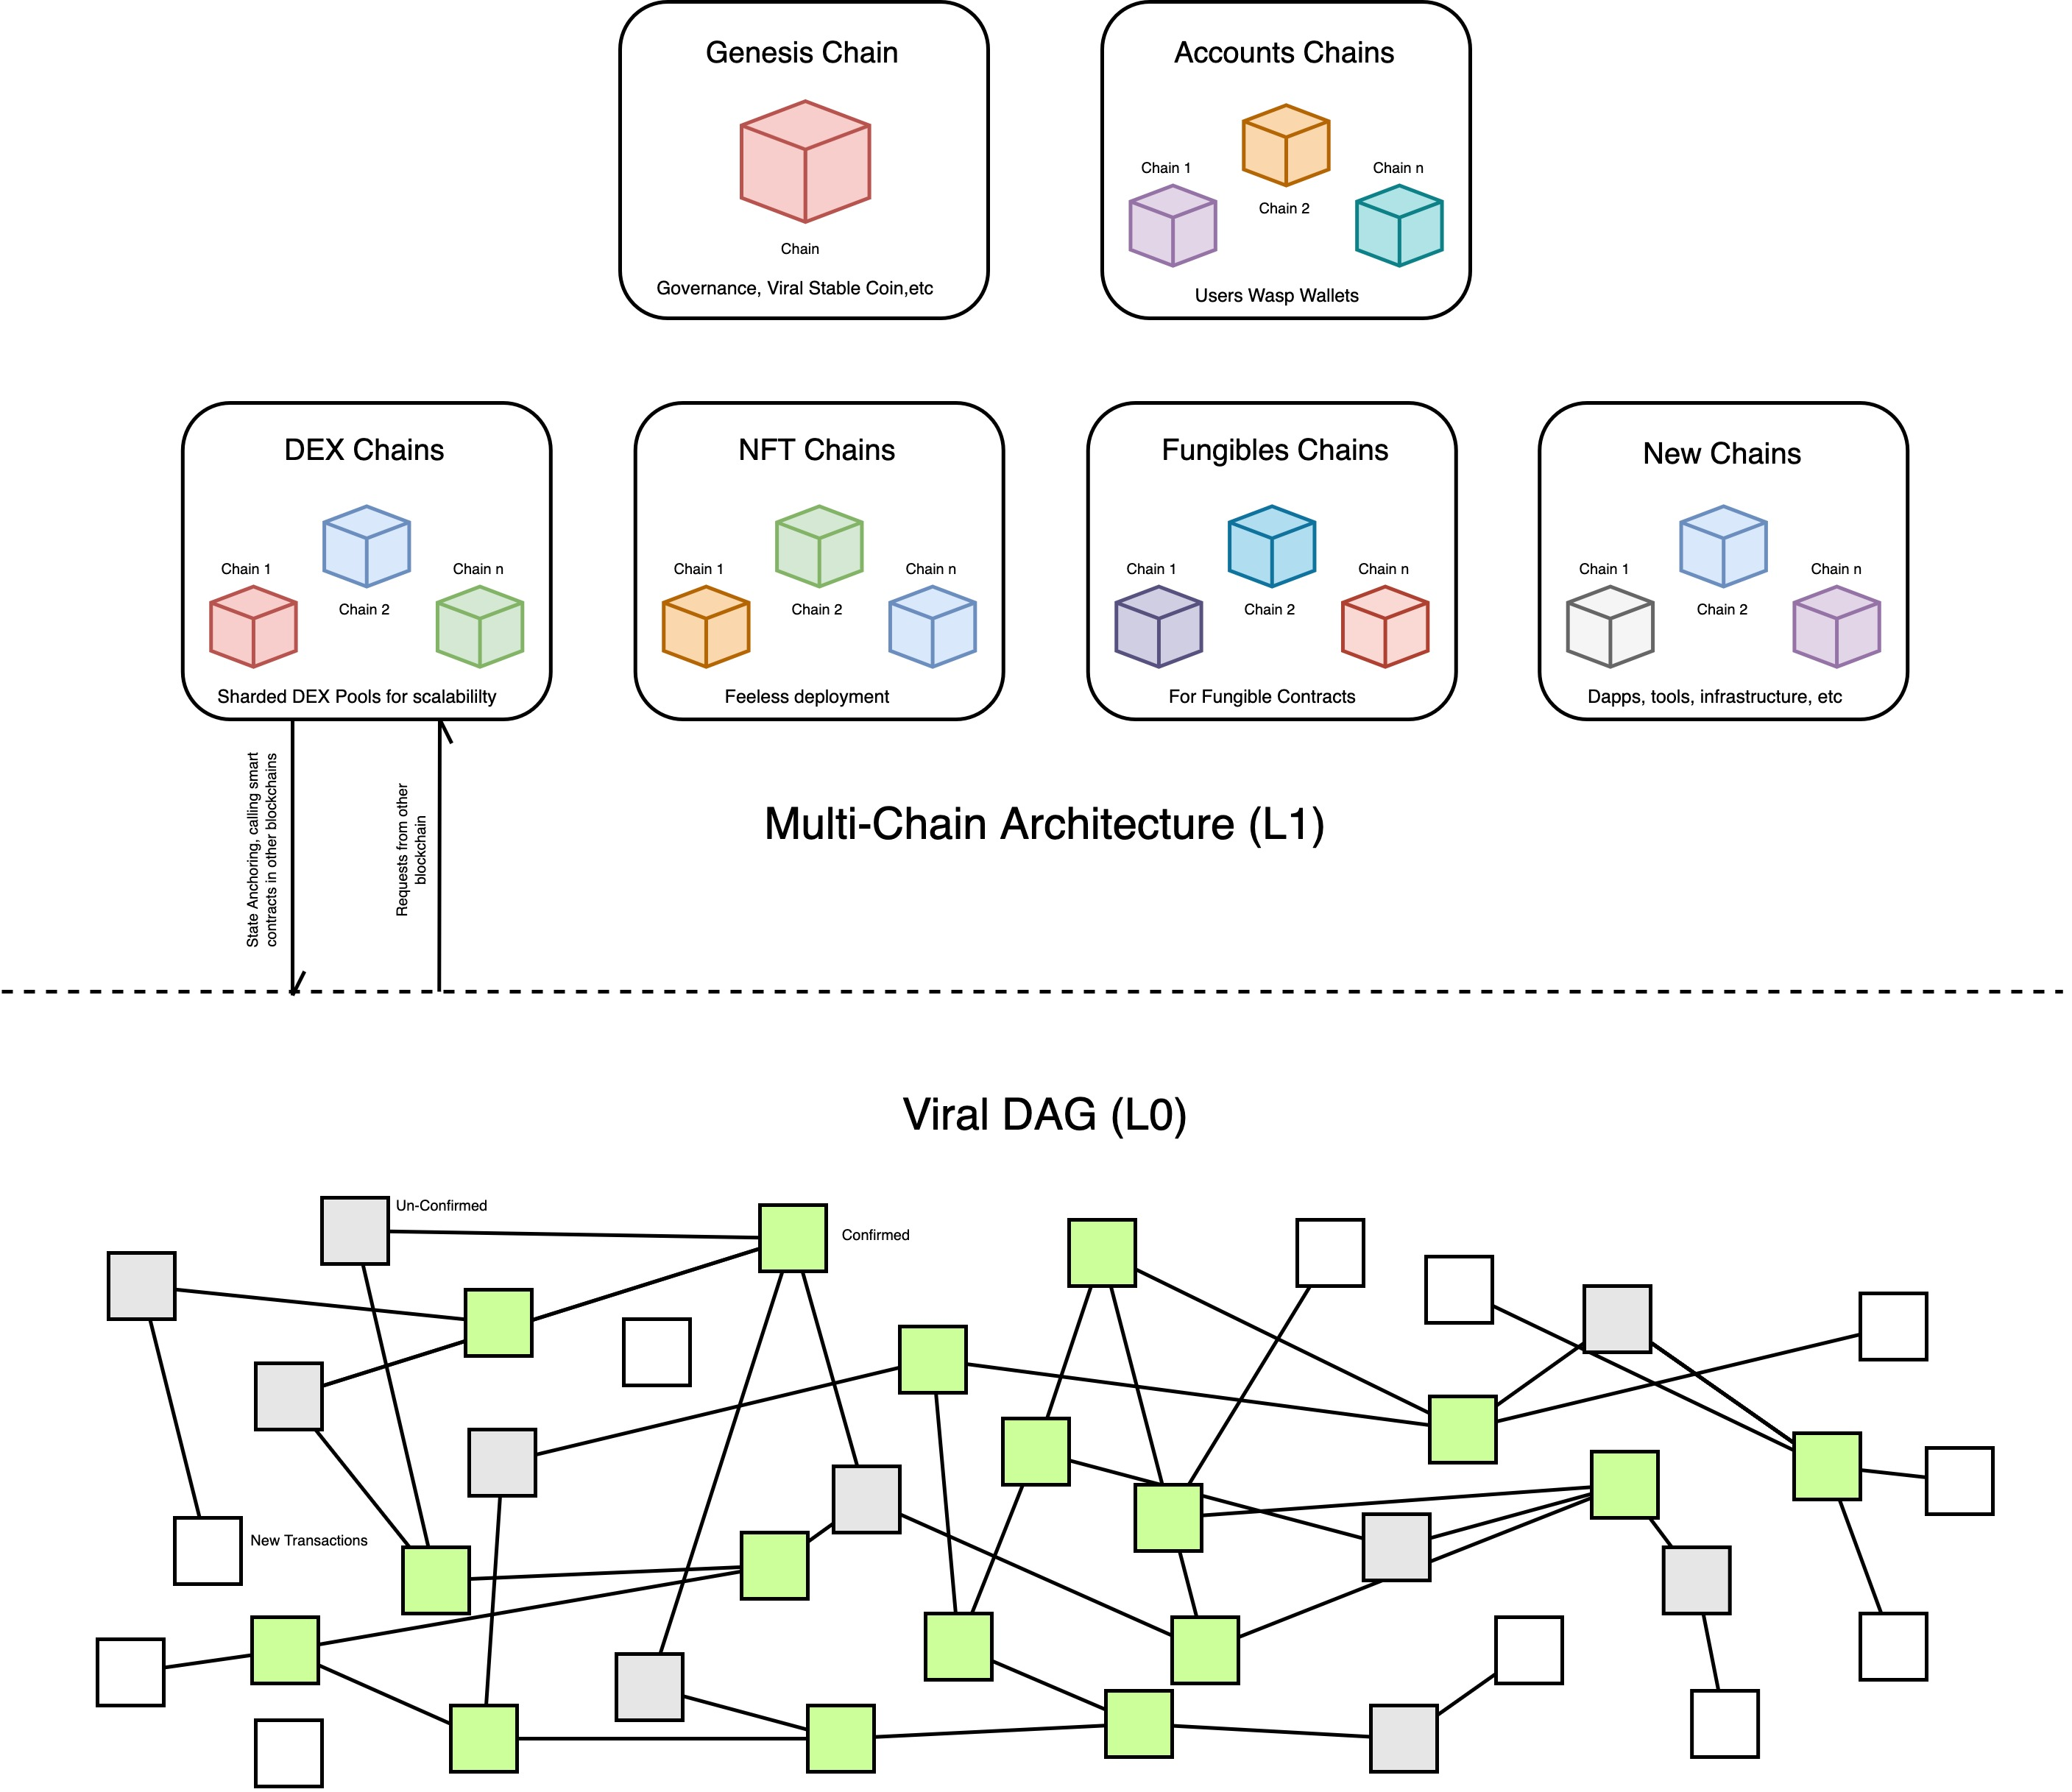
\includegraphics[width=14cm]{Architecture}
\caption{Viral Multi-Chain ELI9 Architecture}
\end{center}
\end{figure*}

Viral Smart Chains are a family of separate chains anchored to the IOTA's Tangle where each chain can communicate with each other via intermediary L1 Value Tangle.\\

\textbf{Viral's Approach}\\

A Single chain will seem complex for setting different fees for different actions on the blockchain i.e Smart Contract Calls/Deployment, Sending Tokens to other Address, etc. Viral's approach is to bring multiple chains categorized by its purpose to serve the Viral Application with fee structure thereby also creating separate chains to provide zero network fees for minting NFTs on Viral App (ERC721 and ERC1155) while rewarding the validators of all Viral chains (including zero fee chains) from the miner pool (total collected fees of all chains) based on validator's total validated transactions for the day through an automated smart contract.\\

\textbf{Family of Chains}\\

\begin{itemize}[wide, labelwidth=!, labelindent=0pt]
\item \textbf{Genesis Chain} : Initialization of First Chain with Viral Coin and Stable Coin Deployment with Smart Contracts that defines governance, fees, etc\\

\item \textbf{Accounts Chains} : For Every n number of active Viral Wallet users a new general chain is deployed. These chains are used to store user funds and create new accounts on the blockchains. So Users can do intra and inter chain transactions with high throughput and flexible scaling.\\
\end{itemize}

\textbf{De-Fi Chains}\\

Smart Contract Deployment Chains specifically for categorized DApps
\begin{itemize}[wide, labelwidth=!, labelindent=0pt]

\item \textbf{DEX Chain} : Running smart contracts for Viral Wallet's Decentralized Exchange

\item \textbf{ERC20 Chain} : To Deploy new ERC20 Tokens that can be transacted between chains and accounts

\item \textbf{Viral NFT Chain} : Feeless Viral ran Smart Contract Chain specifically to deploy user's NFTs on-chain

\item \textbf{ERC721/115 Chain} : To deploy new Non-Fungible Tokens for other platforms outside the Viral Application

\item \textbf{Marketplace Chain} : To create smart contract based marketplaces for NFTs and much more

\item \textbf{Viral DAO Chain} : For Viral DAO Governance contracts

\item \textbf{Other Chains} : For creating Dapps for lending, asset tokenization, yield farming, tools and infrastructure, etc
\end{itemize}

\textbf{Consensus}\\


\textbf{Validators}\\

Viral Chains will require validators to stake their Viral Coins in order to participate in the network for validating transactions. Chance of validating transactions depends on the amount of coins a validator is stakes. Participants who stake more Viral Coins will be most likely to be chosen to add more blocks. When a transaction is validated and attain consensus by the quorum of validators (Read IOTA Protocol), the state of the transaction/smart contract will be recorded in the Value Tangle's UTXO Ledger which makes the state immutable and impossible to fork. The Transaction will be secured by the validators inside the Viral chain and also the L1 UTXO Ledger.\\

\textbf{Permisionless Validators}\\

\textbf{Wasp Nodes}\\

\textbf{Immutable State Anchoring}\\

\textbf{Core Chain Contracts}\\

\textbf{Chain Ownership}\\


\textbf{On-Chain Accounts}\\





\textbf{Fees}\\

Viral Smart Chain is built primarily to ease the need for gas-based transaction fees like other smart contract blockchains. Transaction fees are only leaved as a fixed percentage as transfer fee in Viral Smart Chains for Sending, receiving tokens between accounts and smart contracts. Transfer fees are fixed at 0.05\% of transfer value of the tokens paid in Viral native coin. The minimum fee is capped at \$0.0005 of the fiat value of Viral Coin which is determined using price oracles. While these fees aren't set for all the Viral Smart Chains, different blockchains served for different purposes will require different fee model. Fee model can be intialized in each chain while deploying the governance core-contracts. Such fee model is proposed below\\

\textbf{NFT Chains}\\

Currently on popular smart contract blockchains such as Ethereum, Polygon the amount of gas required for a transaction is determined by the demand for the transaction to be included, regardless of what type of transaction it is where it is dynamically adjusted based on number of user's interacting with the network at the time.\\

This brings us to an effect that a single blockchain cannot set certain fees or eliminate gas fees for a particular type or category of a transaction regardless of it's nature i.e, smart contract, account transfer. Multiple parallel state blockchains can solve this issue by altering few blockchains as permissioned for a certain use cases and can make it feeless without hindering the other fee-based chains.\\

Viral's aim to democratize NFT to the masses and bring massive NFT Adoption we will be running separate zero-fee chains for deploying ERC721 and ERC1155 Token directly from the Viral Application. The Validators for the chain will be open to join the network where they'll be rewarded from the miner pool (total fee collected) based on the total transactions they validate in a day.\\


Development

\begin{lstlisting}

      _Root_

      - _Initialization of the chain_
      - _Deployment of new contracts_
      - _Registary of contracts_
      - _Chain ownership management and Access control list_
      - _Fee management_

      _Accounts_

      - _On Chain ledger accounts_
      - _Securely moving tokens between accounts_
      - _Ensuring consistency of the on-chain ledger_

      _Eventlog_

      - _Keeping timestamp immutable log of On-Chain events_

      _Blob_

      - _Keeping registry of Binary objects of arbitrary sizew_

      _Configuration of Committee and quorum_

      _Wasp Nodes_

      _EVM Plugins_

      _Configuring Fees_

      _Smart Contract Deployments_

      _State Updates on Tangle_

      _Multi-Chain Integration_

      _Core-Contracts_

\end{lstlisting}

\section{\textbf{Viral Token Ecosystem}}

Intro to Viral Token Ecosystem\\
Different Types of Tokens in Viral, its advantages, disadvantages and need\\
Intro to VRL Token and its use cases inside the block-chain\\
Intro to VSC Token\\
Need for stable coin\\
Types of Stable Coin\\
Gold Backed Stable Coin and its advantages over fiat currencies\\
Charts and Statistics about Inflation, PP, and CPI\\
Stability of Fiat over Gold, How fiat is bad and how gold is better\\
Bull and Bear Run of existing gold in history\\
Risks and complexity of reserving physical gold\\
Methods to buy gold\\
Minting VSC\\
Redeeming Reserves of VSC\\
Decentralizing / Diversifying the reserves\\
Need for Fiat Coins amidst Gold Stable Coin\\
Introduction to Viral Fiat Stable Coins\\
Advantages of Both Centralized and Decentralized\\
Easy Liquidity\\
Minting of Fiat Coins\\
Burning of Fiat Coins\\
VSC as a stable collateral\\
Stability over popular collateral coins ETH vs VSC\\
Risks of similar collateral stable coins\\
Statistics and data\\
Minting/Borrowing Fiat Stable Tokens\\
Debt positions and collateral percentages\\
Repayment for debt Redeeming Viral Stable Coin (Gold)\\
Discounted Collateral Auction\\
Overcollateralization of VSC\\
Price Stability by Arbitraging Opportunities\\
Centralized Tokens Collateral Options\\
Risk Factors for Fiat Tokens\\
Constant Decline of All collateral\\
Not Sold Auction for Undercollateralized Assets\\
Freezing of Centralized assets by Governments\\
Benefits of Viral Fiat Stable Coins\\

\section{\textbf{Decentralized Block-chain Bridges}}

With over 12,000 active cryptocurrencies residing in more than 1,000 of public blockchains, the protocols that run the blockchain differ from each other that hinders the interoperability aspect that is very well needed for communicating between blockchains for asset transfers, etc. Most of the tokens are built on Ethereum but due to scalability and higher gas fee issues most developers prefer better-built, faster, more scalable blockchains and sidechains such as Solana,Polygon, Binance, Avalanche. While Ethereum blockchain features a basket of de-fi tokens which involves Fiat-backed/Crypto-backed/Algorithmic Stable-Coins and specific vision-focussed tokens, emerging new public blockchains suffer by not offering a vast options of tokens for the native asset owners. This creates an urgent-need to introduce existing assets on popular blockchains to new public blockchains through cross-chain technologies known as bridges. The availability of such assets restricted to a single blockchain impedes the free-circulation of assets which absolutely delays the value creation which is possible by offering the assets to other platform i.e., blockchain users. With proper cross-chain technologies the inception of multi-token economy shall begin where users can define their choice of tokens without sticking to a specific cryptocurrency as the "One" Internet currency.\\

\textbf{Centralized Exchanges and Multi-Token Wallets}

\textbf{Intro to Cross-Chain Bridges}\\

Trustless vs Trusted Bridges and it's advantages and disadvantages\\

Viral vision to decentralization\\

Risks of Trustless Bridges\\

Recent Bridges hacks\\

RenVM H2H Protocol\\

Why RenVM\\

List of Currently available Chains and Tokens\\

Future Cases\\

Viral's approach\\

Integration of RenVM into Viral Smart-Chains\\




\section{\textbf{Viral Pay - Smart Wallet}}

From early days of bitcoin, crypto wallets serves the one-stop solution to hold and transfer cryptocurrencies through an easy user experience model. There is so much to crypto wallets other than holding coin. Wallets can send, receive digital money, store NFT collectibles, connects to exchanges and a lot more to be integrated in the upcoming future, probably your one account hub for everything in the internet. In,short wallet applications are a place to store your cryptocurrencies securely. 

\begin{figure}[H]
\begin{center}
\begin{forest}
  forked edges,
  for tree={edge+={-Latex}},
  [Crypto Wallet
    [Non-Custodial
        [Hot Wallet]
        [Cold Wallet]
        [Paper Wallet]
    ]
    [Custodial
    ]
  ]
\end{forest}
\caption{Types of Wallet}
\end{center}
\end{figure}


Wallets are classified into centralized custodial wallets and decentralized non-custodial wallets. Decentralized wallets offer high security and total freedom, while custodial wallets in exchanges comply to regulations. Hot wallets are non-custodial wallets that's always connected to the internet and the blockchain network using various APIs to send, receive, view tokens  easily through a browser or a mobile application. Cold wallets are offline physical wallet devices that stores tokens in a storage device i.e., USB Drive that is secure to over the internet attacks. Viral provides hot wallet services to users through an integrated wallet application inbuilt inside the social application.\\ 

\textbf{Pros of Hot Wallets}
\begin{enumerate}[wide, labelwidth=!, labelindent=0pt]
\item \textbf{Access assets anywhere} : Hot wallets provide you the ability to access user's digital assests anywhere, using compact mobile/browser applications
\item \textbf{Free to use} : It takes zero cost to create a wallet address and generate private keys to access the wallet
\end{enumerate}

\textbf{Cons of Hot Wallets}
\begin{enumerate}[wide, labelwidth=!, labelindent=0pt]
\item \textbf{Loss of Private Keys} : Since Non-custodial wallets are decentralized user will hold his private keys and no banks or intermediary custodians will hold on behalf of them. This puts an undeniable risk of losing a cryptographic key or a mnemonic phrase.
\item \textbf{Less Secure than Cold Wallet} : Hot wallets are connected to internet which leaves a vulnerability of potential hacks and threats unlike a cold storage which stores tokens offline.
\end{enumerate}


\textbf{Viral Smart Wallet}\\

Viral Smart wallet is an integrated open-source EVM based hot wallet application that is used to store, send, receive, by \& sell Viral ecosystem of tokens and also used to receive rewards for their contribution towards the decentralized network. Users can create, import multiple wallets and get access to fiat-exchange, decentralized swap pools and zero fee L2 transfers for micro-transactions. \\

Types of Viral-Wallets and Benefits\\

Viral Name Systems\\

Sending \& Receiving Tokens\\

Making De-Fi transactions\\

Security \& Privacy of Wallet\\

Recovery Systems of Viral Wallet\\

Risks of Wallets\\

Features\\

Tap to Pay\\

Transaction Signature Procedures\\

Device Encryption\\

Simple UI and UX\\

Contacts \& Local Business Search via Location\\

Viral Name Search\\

Automated Marked-Crypto Receive Settings\\

Auto VSC Exchange\\

Integrated Viral Exchanges and Viral DAO's DApps\\

Integrated KYC Feature for Fiat Deposit\\

\textbf{QR Pay}\\

The need for faster transactions is rising higher every year and new technologies have been introduced such as NFC, Scan Code, etc. Since Viral Wallet is a crypto wallet, it will be hard for people to use a public address to send and request Viral Coins or other cryptocurrencies to Merchants using the Smart Wallet . QR Pay is a feature to be added on the Smart Wallet to facilitate faster recognition of seller’s wallet address and the amount to be transferred by scanning a simple generated QR Code through Viral Application. This QR Pay will come when the user doesn’t know their username and want to request money from a nearby person. This will be helpful for businesses to collect payment from users swiftly by entering the amount needed to be paid.\\

\section{\textbf{Viral Decentralized Exchanges}}

Decentralized exchanges (DEX) are a type of cryptocurrency exchange that allows for direct peer-to-peer cryptocurrency transactions to take place online securely and without the need for an intermediary or a custodian, unlike Centralized exchanges. Decentralized exchanges are simply a set of automated smart contracts (code). They establish the prices of various cryptocurrencies against each algorithmically and use “liquidity pools” — in which investors lock funds in exchange for interest-like rewards — to facilitate trades. While transactions on a centralized exchange are recorded on that exchange’s internal database, DEX transactions are settled directly on the blockchain itself. There will be no custodian or any services which need to be maintained by a certain company to run a truly decentralized crypto exchange.DEXs are usually built on open-source code, meaning that anyone interested can see exactly how they work. That also means that developers can adapt existing code to create new competing projects — which is how Uniswap’s code has been adopted by an entire host of DEXs with “swap” in their names like Sushiswap and Pancakeswap.\\

\textbf{Automated Market Makers}\\

An automated market maker (AMM) is a type of decentralized exchange (DEX) protocol that relies on a mathematical formula to price assets. Instead of using an order book like a traditional exchange, assets are priced according to a pricing algorithm.This formula can vary with each protocol. Most AMMs usesa constant product formula: $x  \times  y = k$, where $x$ is the amount of one token in the liquidity pool, and $y$ is the amount of the other. In this formula, k is a fixed constant, meaning the pool’s total liquidity always has to remain the same. Liquidity providers (LPs) add funds to liquidity pools. In return for providing liquidity to the protocol, LPs earn fees from the trades that happen in their pool. LPs deposit an equivalent value of two tokens – for example, 50\% of Token A and 50\% of Token B to the A/B Lquidity pool.\\

\textbf{Pros of AMMs}
\begin{enumerate}[wide, labelwidth=!, labelindent=0pt]
\item \textbf{No KYC Procedures}: Decentralized exchanges are similar to peer-to-peer exchanges but rather taking from an individual the user can withdraw funds from a trustless liquidity pool that requires no ID verification and other complex processes
\item \textbf{Secure} : DEXs are secure as the funds are withdrawn, deposited and held on-chain through smart contracts that is secure and immutable
\item \textbf{Non Custodial}: Liquidity Providers can provide liquidity and withdraw them whenever they need to, making it a non-custody protocol where user's funds will be held on a smart contract rather than a central custodian.
\item \textbf{Zero Manipulation}: Since user's funds are stored in a trustless manner, the smart contracts cannot freeze any account, transfer data to anyone nor manipulates price like a centralized exchange
\end{enumerate}

\textbf{Cons of AMMs}
\begin{enumerate}[wide, labelwidth=!, labelindent=0pt]
\item \textbf{Scalability}: Various DEXs are suffered from network congestions which delays the execution of trades. This is been solved by making DEXs on top of scalable high throuoghput blockchains, but the DEXs are limited to the scalability of the blockchain itself and cannot scale on it's own.
\item \textbf{Price Impacts}: Price impact is the influence of user's individual trade over the market price of an underlying asset pair. It is directly correlated with the amount of liquidity in the pool/Automated Market Maker (AMM).
\item \textbf{Limited Functions}: AMM based DEXs offers only to execute buy and sell orders and doesn't offers advanced trading features like limit orders aren't available on current exchanges.
\item \textbf{Volatility}: As price impacts being created, on an illiquid trading pair the volatility always reach new highs to stabilize the constant $k$ in the constant product formula $x \times  y=k$ to satisfy demands. This creates high volatile market while user's only use DEXs go for high liquid, low volatile market.
\item \textbf{Impermanent Loss}: Impermanent loss describes the temporary loss of funds occasionally experienced by liquidity providers because of volatility in a trading pair. Liquidity Providers suffer negative returns comparing to holding tokens outside the pool. Volatility and Price Impacts are the major aspects of impermanent loss. The loss becomes permanent if a provider decides to withdraw their liquidity from the pool.
\end{enumerate}

\textbf{Problem 1 : Price Impacts \& Volatility in AMMs}\\

The difference between the current market price and the price a user will pay to perform a swap in a decentralized exchange is known as Price Impacts. This happens when the ratio of the assets in the pool changes where one asset is more liquid and another is illiquid. When a large swap is conducted a maximum portion of the swapped asset is erased from the liquidity pool, supplying more of the provided asset, to maintain the $k$ of the constant product formula $x \times y=k$ the smart contract will ask for a increased supply of tokens to balance the $k$. This will create a impact on the current price, making the trade much more expensive than centralized trades and spiking the volatility of the pool.\\



For example., Two Coins $X$ and $Y$\\

\textbf{Pool Info/Before Swap}:
\begin{itemize}[wide, labelwidth=!, labelindent=0pt]
\item Before Swap $X$=20
\item Before Swap $Y$=45,000
\item Constant Product $K=X \times  Y$ = 900,000 
\item Before Swap Price $M=\frac{Y}{X}$ = 2,250 
\end{itemize}

\textbf{Trade $n$}: $n$= 9,000 y for x\\

\textbf{After Swap}:
\begin{itemize}[wide, labelwidth=!, labelindent=0pt]
\item After Swap $Y_n$=54,000 
\item Constant Product ($K$) = 900,000 (Stays Same)
\item After Swap $X_n=\frac{K}{Y_n}$ = 16.666  
\end{itemize}
\textbf{Results}:
\begin{itemize}[wide, labelwidth=!, labelindent=0pt]
\item Received $X_f={{X}-{X_n}}$ = 3.334 
\item Price paid per X / After Swap Price $M_n={\frac{n}{X_f}}$  = 2,699  
\item \textbf{Price Impact} $P={\frac{M - M_n}{M} \times  100}$ = \textbf{19.95\% }
\end{itemize}


\textbf{Conclusion}:\\

To take 9,000 Y Tokens from XY Pool having 20:45000 Tokens, user have to pay \textbf{19.95\% more} than the market price. \textbf{Market Price = 2,250} , \textbf{User Price = 2,699}\\


Huge price impacts happens only in pools that has less liquidity when a maximum percentage of a token in a pool is withdrawn. These price impacts are being neutralized by arbitrage traders who buys token at lower prices on other exchanges and sell the same token high on decentralized exchanges which will has a maximum price impact, these arbitrage traders will continue to make trades for profits until the market price is achieved. Although arbitrage traders are available to minimize the price impacts, users cannot always wait for the arbitragers to stabilize the pools. DEX aggregators offer users a better solution by buying the token across all pools in order to minimize price impact on each one of them. Instead of spreading the trade over time in a single market, this order executes at once, spread over many possible markets. Aggregators also command substantially higher gas costs than a single trade, similar to splitting trades manually. To conclude there are different secondary solutions that minimizes the price impact through secondary trades (trades after the price impact maximizes), the first trader after it neutralizes will always execute orders with price impacts and slippage of prices while multiple trades happen in the middle.\\

\textbf{Problem 2 : Limited Functions}\\

Order book centralized exchanges offers advanced trading features such as limit orders where traders can bid and ask at different prices from the current market prices. DEXs doesn't offer limit orders and only offers instant market orders with a possible price impact. Order book exchanges are better in terms when it comes to live exchanges and better prices for buying and selling. AMMs has its own benefit compared to order books by providing liquidity at anytime regardless of number of orders.\\

\textbf{Problem 3 : Impermanent Loss}\\

Impermanent loss is the most common loss a liquidity provider experience and a risk of using Automated Market Maker (AMM) based Liquidity Pools. Impermanent loss deals with pairs of the liquidity pools, usually while contributing to a liquidity pool a liquidity provider shall equally provide both tokens according to it's market price that will determine the liquidity providers share of the pool in percentage. For example in a pool of XY Tokens for every X token \$100 tokens of Y should be provided taking Y token as a Stable Coin with Y=\$1, when a LP provide 1:100 worth \$200 to the pool with a final ratio of 10:1000 has 10\% of the pool where the LP will be rewarded extra with the transaction fees (usually 0.3\%) according to the percentage the the LP holds. To represent his liquidity the LP will be offered with LP Tokens of the specific pool which the LP can claim and withdraw his tokens.\\

When trades happens the volatility of the two pairs is a nightmare to LPs due to changes in prices that leads to impermanent losses. Impermanent losses are not permanent until the LP withdraw his pool's liquidity. From the above example after the LP provided XY Tokens with 1X = 100Y if the price of X token appreciates to 1X = 400Y, the ratio of the pool would haved changed to 5:2000 maintaining the constant of total liquidity. When the LP withdraws his tokens from the pool he is entitled to his 10\% of funds withdrawing 0.5X and 200Y which totals to \$400. The LP made a profit of \$200, but would have gained more by simply holding the funds of 1X and 100Y worth \$500. The losses compared to holding and providing to a liquidity pool is often termed as impermanent loss but sometimes will be substituted by trading fee rewards. Effects of huge price volatility and impacts creates impermanent losses of LP's funds.\\

\textbf{Problem 4 : Scalability of DEXs}\\

Decentralized exchanges suffer greater scalability issues during frequent network congestions of blockchains. The scalability of DEXs is directly related to the scalability of blockchains. Without a highly scalable blockchain DEXs cannot prepare for a mainstream adoption where trading volume would increase by radical margins.\\

\textbf{Solution to Current Risks}\\

Current AMMs gives the opportunity for non-simultaneous series of buys and sells where two traders can buy A tokens freely which will increase the price impact thereby making the pool's token price to change drastically compared to the original market price. To eliminate price impacts for the next buyer (buy-buy trade) the following swaps (next swap order) should be opposite to the previous swap (sell) i.e., While first swap takes A tokens for B , the following trade should be taking B tokens for A, thereby minimizing price impact by stabilizing the pool for the next (buy) traders. A simultaneous matching of buyers and sellers can minimize the price impact for the next set of buyers and sellers. This matching is in centralized exchanges are done through order books where it matches traders for their input price .i.e, a limit order. The solution is to maintain a swap book on top of the liquidity pool to match buyers and sellers to maintain the stability of the pool and eliminate price impacts.\\

\begin{figure*}
\begin{center}
\begin{tabularx}{\textwidth} { 
  | >{\centering\arraybackslash}X 
  | >{\centering\arraybackslash}X 
  | >{\centering\arraybackslash}X 
  | >{\centering\arraybackslash}X 
  | >{\centering\arraybackslash}X 
  | >{\centering\arraybackslash}X 
  | >{\centering\arraybackslash}X 
  | >{\centering\arraybackslash}X 
  | >{\centering\arraybackslash}X
  | }
 \hline
 \textbf{Sl.no} & \textbf{Type} & \textbf{Buy} & \textbf{Sell} & \textbf{Trade Price (per A)} & \textbf{Price Impact (from Market Price = 2)} & \textbf{Pool Ratio}\\
 \hline
 1 & Buy & 20A & 50B & 2.5  & +25\% & 80/250   \\
  \hline
 2 & Buy & 10A & 35.7B & 3.5  & +75\%  & 70/214.2   \\
  \hline
 3 & Sell & 10B & 27.9A & 0.3  & -85\%  & 97.9/204.2   \\
  \hline
 5 & Sell & 10B & 5A & 0.5 & -75\% & 102.9/194.2   \\
\hline
\end{tabularx}
\caption{Example of Simultaneous AMM Orders on current DEXs using Constant Product Formula on low liquidity pools}
\end{center}
\end{figure*}


While conducting an alternate(buy-sell) swap, it leaves significant price impacts on either of the trades for maintaining the $k$ in the Constant Product Formula $x \times  y=k$, it will not be useful to minimize the price impacts by doing two trades one after each other. Also when two trades match it is best in case to make a decentralized atomic swap instead of taking from a Liquidity pool that will revert to it's previous pool price before the trade. This comes to a conclusion that Traders with matching swaps doesn't provide any results for reducing price impacts, changing the pool's price to market price, etc.\\


To give solution to all the existing AMM risks and problems we should be allowing traders to only withdraw if they match with their corresponding opposite trader (buy-sell) while changing the traders buy/sell amount to change the pool's price to market price by traders acting as a smaller liquidity providers. \\

\begin{figure}[H]
\begin{center}
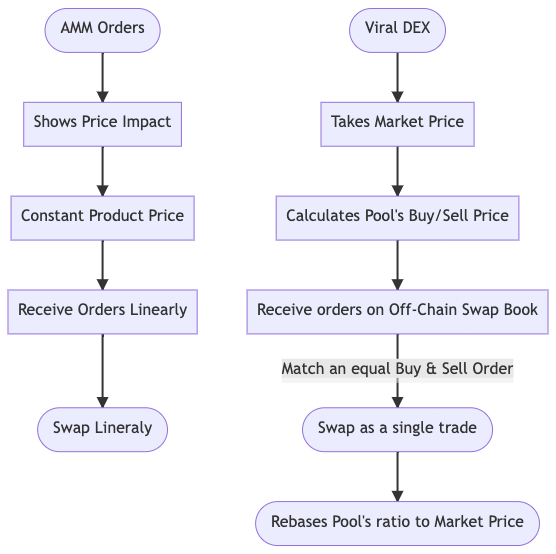
\includegraphics[width=7cm]{dex}
\caption{AMMs vs Viral DEX}
\end{center}
\end{figure}

\begin{comment}%mermaid
graph TD


    A([AMM Orders])
    C[Shows Price Impact]
    Z[Constant Product Price]
    D[Receive Orders Linearly]
    E([Swap Lineraly])

    A-->C-->Z-->D-->E
    F([Viral DEX])
    G[Takes Market Price]
    H[Calculates Pool's Buy/Sell Price]
    I[Receive orders on Off-Chain Swap Book]
    K([Swap as a single trade ])
    L([Rebases Pool's ratio to Market Price])

    F-->G-->H-->I--Match an equal Buy & Sell Order -->K-->L

    

\end{comment}

\textbf{Intro to Viral DEX}\\

Viral DEX is a Liquidity Pool exchange that matches buyers and sellers through it's swap book on top of it's Liquidity Pools while automatically rebasing the pool to it's live market's price thereby minimizing price impacts and proving faster and scalable trades using its micro-pool architecture\\

\textbf{Swap Book}\\

An Off-Chain Swap book similar to an order matching book will match buyers (Buy Primary Coin) and sellers (Buy Secondary Coin) and commence orders to a liquidity pool to swap between tokens. This order book is maintained on top of a liquidity pool to reduce price impacts and give a fair price for each token swap near to market price. 

\begin{figure}[H]
\begin{center}
\begin{tabularx}{0.5\textwidth} { 
  | >{\centering\arraybackslash}X 
  | >{\centering\arraybackslash}X 
  | >{\centering\arraybackslash}X 
  | >{\centering\arraybackslash}X | }
 \hline
 \textbf{Sell B} & \textbf{Buy A} & \textbf{Sell A} & \textbf{Buy B}\\
 \hline
 48.929687  & 1  & 0.43  & 21.869531\\
  \hline
 19.571875  & 0.4  & 0.946  & 48.112968\\
  \hline
 63.608593  & 1.3  & 0.344  & 17.495625\\
  \hline
 0.978593  & 0.02  & 1  & 50.859375\\
   \hline
   \hline
 133.088748  & 2.72  & 2.72  & 138.337499\\
\hline
\end{tabularx}
\caption{An Example Swap Book}
\end{center}
\end{figure}

To read a swap book one must need to determine the primary (A) and secondary Token (B). The token which has more value (typically in dollars) is a primary token compared to the lesser value secondary token. The buyers of primary tokens and sellers of secondary tokens are collectively considered as \textbf{Buyers} and the sellers of primary tokens and buyers of secondary tokens are considered as \textbf{Sellers}.

\begin{figure}[H]
\begin{center}
\begin{tabularx}{0.5\textwidth} { 
  | >{\centering\arraybackslash}X 
  | >{\centering\arraybackslash}X 
  | >{\centering\arraybackslash}X 
  | >{\centering\arraybackslash}X | }
 \hline
 Sell DAI & Buy ETH & Sell ETH & Buy DAI\\
\hline
\end{tabularx}
\caption{Example of an ETH/DAI Swap Book}
\end{center}
\end{figure}

Swap books contains prices derived from liquidity pool's current price and the trading pair's market prices. These continuous swaps determine the execution of orders into the liquidity pool and rebases the current liquidity pool's price to market price.\\

\textbf{Pricing Strategy}\\

In AMMs prices of swaps determined by the constant product formula $x \times  y=k$ where to swap $x$ tokens the liquidity pool will simulate the pool's after trade liquidity and by maintaining the $k$ constant it determines the amount of $y$ tokens a trader must provide. Whereas, in Viral DEX the constant product formula isn't used. Viral's Liquidity Pool execution of providing pool's liquidity will always require two simultaneous buy and sell of tokens with an addition of extra tokens to change the current price of pool to market price.


\begin{center}
$Current\:Price\:of\:A = \frac{B}{A}$
\end{center}

A Pool's current price is determined by the ratio of the total tokens in the liquidity Pool. Since the current price isn't derived exactly from the market price, it might vary. Usual AMMs doesn't promises buy and selling of tokens in market rates, rather it is manually rebased to current market prices by arbitrage traders. Viral DEX doesn't provides the current buy price and sell price by calculating the ratio, rather it calculates the difference between the current market price and the current pool price and determines the buy and sell prices with conditions that can make the pool rebase to it's market price automatically when trades execute.\\

The Buy and Sell Price will always in regards to the market price because of the Viral's constant rebasing mechanism. The difference of market and current price is calculated by subtracting both prices. For Example in a ETH/DAI pool of ratio 5:2000 the current price is $\frac{B}{A}=\frac{2000}{5}=400$ where if the market price rose to 402 then the difference would be $Market\:Price - Current\:Price=402-400=2$

\[Difference\:D = Market\:Price - Current\:Price\]



Thus a difference is taken into account to determine the buying and selling price of the current pair to rebase the price. The buy and sell price is determined by whether the difference is positive or negative. During bull market the difference will come in a positive integer when the $M.P>C.P$ market price is more than current price. Here the buy price of primary token will be added with the difference, where the sell price is the current price. During bear market the difference will come in a negeative integer when the $M.P<C.P$ market price is lesser than current price. Here the buy price of primary token will be the current price, where the sell price will be calculated by subtracting the difference\\

If D = positive $+$

\[Buy\:A=Current\:Price+Difference\]

\[Sell\:A=Current\:Price\]

If D = negative $-$

\[Buy\:A=Current\:Price\]

\[Sell\:A=Current\:Price-Difference\]



\textbf{Example Problem}\\

To understand how prices are calculated let's take an example problem. Find the pool's current price, buy \& sell price and difference while it's market price is less than 5\% of it's current price\\

\textit{Given} : Pool = 256/12526\\

Here C.P = Current Price , M.P = Market Price\\

Given A = 256 , B = 12526 ;
To find current price 

\[\text{C.P\:of\:A}=\frac{B}{A}=\frac{12526}{256}=\frac{48.9296875}{1}=\frac{B}{A}\]


Currently 1A=48.9296875B\\

Find M.P by subtracting 5\% of C.P $48.9296875 - ((48.9296875)(5\%))$ 

\[\text{M.P} = 46.483203125\]

Now, Find Difference between C.P and M.P $Difference\:D = Market\:Price - Current\:Price$

\[\text{Difference\:D} = -2.446484375\]

If D = negative , $Buy\:A=Current\:Price$, $Sell\:A=Current\:Price-Difference$

\[\text{Buy\:A} = 48.9296875\]

\[\text{Sell\:A} = 51.376171875\]

\textit{Proof}

\[\text{Final\:Price}=\frac{C.P+Buy\:Price - Sell\:Price}{A} = 46.483203125\]

\[Market\:Price=Final\:Price\]

Hence the buy and sell price is found and proved to move the token price to the market price. Similarly when the D (Difference) is positive the outcome will be achieved. \\


\textbf{Conditions and Requirements}\\

In centralized Order Books buyers are matched with sellers on the same price rate where in a swap book an order is executed when the sum of all buyers amount (Buy A or Buy B) should equal sum of all sellers amount (Sell A or Sell B) regardless of which token it is. This is a condition in a swap book for it to execute the order to a Liquidity Pool. Off-Chain Trading engines shall match summations of both buy \& sell amounts randomly and execute order and send funds to the users.\\

\[\sum_{n}^{\infty} BA_n = \sum_{n}^{\infty} SA_n\]


\begin{center}
(or)
\end{center}
\[\sum_{n}^{\infty} BB_n = \sum_{n}^{\infty} SB_n\]

The final index of the summations $\infty$ represents the limit of total number of table rows in the swap book e.g., $BA_1$ represents 1st row and Buy A column. The initial index $n$ indicates the swap book tables rows serial numbers where it's numbers are taken i.e., the swap amounts. The Summation term $BA_n, SA_n, BB_n, SB_n$ represents the addition of values taken from the tables. Here the Equation (12) constitutes that the summation of BA should be equal to summation SA and vice versa to be able to execute the swap. Where Equation (13) constitutes that the summation of BB should be equal to summation SB and vice versa to be able to execute the swap.\\
\onecolumn
\textit{\textbf{Example Swap Order}}\\

A swap order in a Pool ratio of 256:1256 where it satisfies equation (12) to commence an order to the liquidity pool
\begin{center}
A = 256, B= 12526, C.P = 48.9296875, M.P=47,\\
D=-1.9296875, Buy 1 A=48.9296875 B , Sell 1 A=50.859375 B
\end{center}
\begin{figure}[H]
\begin{center}

\begin{tabularx}{0.8\textwidth} { 
  | >{\centering\arraybackslash}X 
  | >{\centering\arraybackslash}X 
  | >{\centering\arraybackslash}X 
  | >{\centering\arraybackslash}X 
  | >{\centering\arraybackslash}X | }
 \hline
 \textbf{Sl.no} & \textbf{Sell B (SB)} & \textbf{Buy A (BA)} & \textbf{Sell A (SA)} & \textbf{Buy B (BB)}\\
 \hline
 1 & 48.929687  & 1  & 0.43  & 21.869531\\
  \hline
 2 & 19.571875  & 0.4  & 0.946  & 48.112968\\
  \hline
 3 & 63.608593  & 1.3  & 0.344  & 17.495625\\
  \hline
 4 & 0.978593  & 0.02  & 1  & 50.859375\\
   \hline
   \hline
 Total & 133.088748  & 2.72  & 2.72  & 138.337499\\
\hline
\end{tabularx}
\caption{Example Swap Book matched order for $\sum_{n}^{\infty} BA_n = \sum_{n}^{\infty} SA_n$}
\end{center}
\end{figure}

\[Final\:Price=\frac{B+\sum SB - \sum BB}{A} = \frac{12526+133.088748-138.337499}{256}= 48.9091845664\]\\

Here the total $\sum BA = \sum SA$ $2.72=2.72$ executes the order and changes the current price of 48.9296875 to  a final price of 48.9091845664 (Eq 14). After this trade the buy and sell price will be changed according to the difference $D=-1.9091845664$ Buy 1A=48.9091845664 and Sell 1A=50.8183691328 to bring the M.P to 47. Until the M.P is achieved the buy and sell price will change after each order execution.\\

Swap book order that satisfies equation (13) to commence an order to the liquidity pool\\
\begin{center}
A = 256, B= 12526, C.P of B = 0.02043749, M.P=0.015,\\
D=-0.00543749, Buy 1 B=0.02043749 A , Sell 1 B=0.02587498 A
\end{center}
\begin{figure}[H]
\begin{center}
\begin{tabularx}{0.8\textwidth} { 
  | >{\centering\arraybackslash}X 
  | >{\centering\arraybackslash}X 
  | >{\centering\arraybackslash}X 
  | >{\centering\arraybackslash}X | }
 \hline
 \textbf{Sell B (SB)} & \textbf{Buy A (BA)} & \textbf{Sell A (SA)} & \textbf{Buy B (BB)}\\
 \hline
 3297.339273  & 85.3185877421  & 39.0858162828  & 1912.45677834\\
  \hline
 2110.29713472  & 54.6038961549  & 47.172536893  & 2308.1374911\\
  \hline
 1187.04213828  & 30.7146915872  & 48.5203236614  & 2374.08427656\\
   \hline
   \hline
 6594.678546  & 170.637175484  & 134.778676837  & 6594.678546\\
\hline
\end{tabularx}
\caption{Example Swap Book matched order for $\sum_{n}^{\infty} BB_n = \sum_{n}^{\infty} SB_n$}
\end{center}
\end{figure}
\[Final\:Price=\frac{A+\sum BA - \sum SB}{B} = \frac{256+134.778676837+170.637175484}{12526}= 0.017574764\]\\

Here the total $\sum SB = \sum BB$ $6594.678546=6594.678546$ executes the order and changes the current price of 0.02043749 to  a final price of 0.0175747644 (Eq 15). After this trade the buy and sell price will be changed according to the difference $D=-0.0025747644$ Buy 1B=0.0175747644 A and Sell 1B=0.0201495288 A to bring the M.P to 0.015. Until the M.P is achieved the buy and sell price will change after each order execution.\\

\twocolumn

\textbf{Liquidity Limits for Rebase}\\

Using Viral DEX's pricing strategy for buying and selling by adding a difference $D$ rebasing, a necessary condition is needed to change the pool's current price to market price. The Total liquidity should be equal to the swap orders total volume i.e., In a 200/100 pool the sum of either buy or sell should attain it's pool's liquidity limit of 200 and 100 Tokens to change the pool to market price. While smaller pools rebases quickly, larger pools usually takes more time to get matched swap orders. To counter this liquidity and swap order issue the concept of Micro-Pools, Time Average Market Price (TAMP), Reserve Pools, Automated Pool Finding Algorithm are implemented.\\

\textbf{Micro Pool Architecture}\\

Viral DEX Pools implies a micro pool architecture for it's unlimited scalability and high throughput on swap orders. Since the protocol implies a swap book which will be matching total buys and total sells, the orders may get delayed in bigger pools which will require higher amounts of matches. Sharding the pools may increase the likeliness of getting matched and execution of users orders on the swap book. \\

Pools are sharded in percentages where the last added micro pool will be divided equally in to two parts $\frac{X}{2}$. This sharding will commence everytime a new blockchain is added to the Viral Smart Chain's -DEX Chains. Pool creators can able to shard their pools into existing number of DEX blockchains.


\begin{figure}[H]
\begin{center}
\begin{forest}
  forked edges,
  for tree={edge+={-Latex}},
  [100\%
    [50\%
		[50\%
			[50\%
				[50\%
					[50\%]				
				]				
				]		
		]    
    ]
    [50\%
    	[25\%
			[25\%
				[25\%
					[25\%]				
				]			
			]    	
    	]
    	[25\%
			[12.5\%
				[12.5\%
					[12.5\%]
				]
			]
			[12.5\%
				[6.25\%
					[6.25\%]				
				]
				[6.25\%
					[3.125\%]
					[3.125\%]				
				]			
			]    	
    	]
    ]
  ]
\end{forest}
\caption{Pool Shards after each new DEX blockchain addition}
\end{center}
\end{figure}

Each Micro-Pool determines each DEX blockchain added to the Viral Smart Chains where smaller pools can get increased volume in smaller transactions. When trade amount is lower the swap book will place the orders in smaller pools which may get matched faster whereas larger trades may get placed in larger pools or the trades will be divided among several pools to get matched and execute the swap successfully \\


The pools are represented in tables with rows mentioning number of pools where each pool will run on different blockchains and columns are represented to determine the cell value and percentage. Here $C_{11}, C_{22}, C_{33}, C_{44}.....C_{rc}$ are the pools that will be separated into two divisions equally ($50\%+50\%$) to form the new pool\\


\begin{figure*}
\begin{center}
\begin{tabularx}{0.9\textwidth} { 
  | >{\centering\arraybackslash}X 
  | >{\centering\arraybackslash}X 
  | >{\centering\arraybackslash}X 
  | >{\centering\arraybackslash}X 
  | >{\centering\arraybackslash}X
  | >{\centering\arraybackslash}X
  | >{\centering\arraybackslash}X
  | >{\centering\arraybackslash}X 
  | >{\centering\arraybackslash}X | }
 \hline
 \textbf{Chains} & \textbf{1} & \textbf{2} & \textbf{3} & \textbf{4} & \textbf{5} & \textbf{6} & \textbf{7} & \textbf{8}\\
 \hline
 \textbf{1}  & 100\% & & & & & & & \\
  \hline
 \textbf{2} & 50\%   & 50\%  & & & & & & \\
  \hline
 \textbf{3} & 50\%   & 25\%  & 25\%  & & & & & \\
   \hline
 \textbf{4} & 50\%   & 25\%  & 12.5\%  & 12.5\%  &  &  & & \\
    \hline
 \textbf{5} & 50\%   & 25\%  & 12.5\%  & 6.25\%  & 6.25\%  & & & \\
     \hline
 \textbf{7} & 50\%   & 25\%  & 12.5\%  & 6.25\%  & 3.125\%  & 3.125\%  & & \\
     \hline
 \textbf{8} & 50\%   & 25\%  & 12.5\%  & 6.25\%  & 3.125\%  & 1.5625\%  & 1.5625\%  & \\
      \hline
 \textbf{9} & 50\%   & 25\%  & 12.5\%  & 6.25\%  & 3.125\%  & 1.5625\%  & 0.78125\% & 0.78125\% \\
\hline
\end{tabularx}
\caption{Micro-Pool Table}
\end{center}
\end{figure*}

\textbf{TAMP - Time Average Market Price}\\

As discussed in the earlier paragraphs the rebases successfully happen only if the trading volume equals the pool's total liquidity. This places a limitation of slower rebases due to the massive segregation of price impacts to every trader who wishes to buy/sell on the trading pair until the total trades rebases. To solve this limitation the concept of Micro-pools and Time Average Market Prices are introduced to traders. Micro-Pools fortunately split up the pools to rebase the smaller pools at first for the retail traders, where the smaller pools will rebase swiftly in real-time than larger pools. To benefit the large pool traders and to eliminate the real-time volatility during constant changes in rebase prices Time Average Market Price (TAMP) is brought out.\\

Each sharded pool will have different market prices derived from real time and delayed market prices in a following time period. Each sharded pool will have a time period configuration which will be determined by the number of DEX chains. For the first sharded pool $50\% + 50\%$ the time period will start with $2 seconds + 2 seconds$ where the market price shall be reflected every 2 seconds and calculated the buy and sell price of the current pool. Since most of the swap orders are instant swaps other than limit orders used by advanced traders, the buy and sell price of the pool will not affect the retail traders which changes every time period specified (in the example 2 seconds) regardless of pending swap orders left in the swap book.\\

Every Pool will have strict time period after which it can able to fetch the market price and update the buy/sell price. For Example., In 5 total sharded pools if Pool 5 has a time period of 16 seconds, the market price will be fetched every 16 seconds once and the buy/sell price will be altered according to the difference in the market and the pool's price. In short, according to the time period the market price is fetched from a decentralized oracle and will be used to determine buy/sell price for rebasing the pool. \\



\begin{figure}[H]
\begin{center}
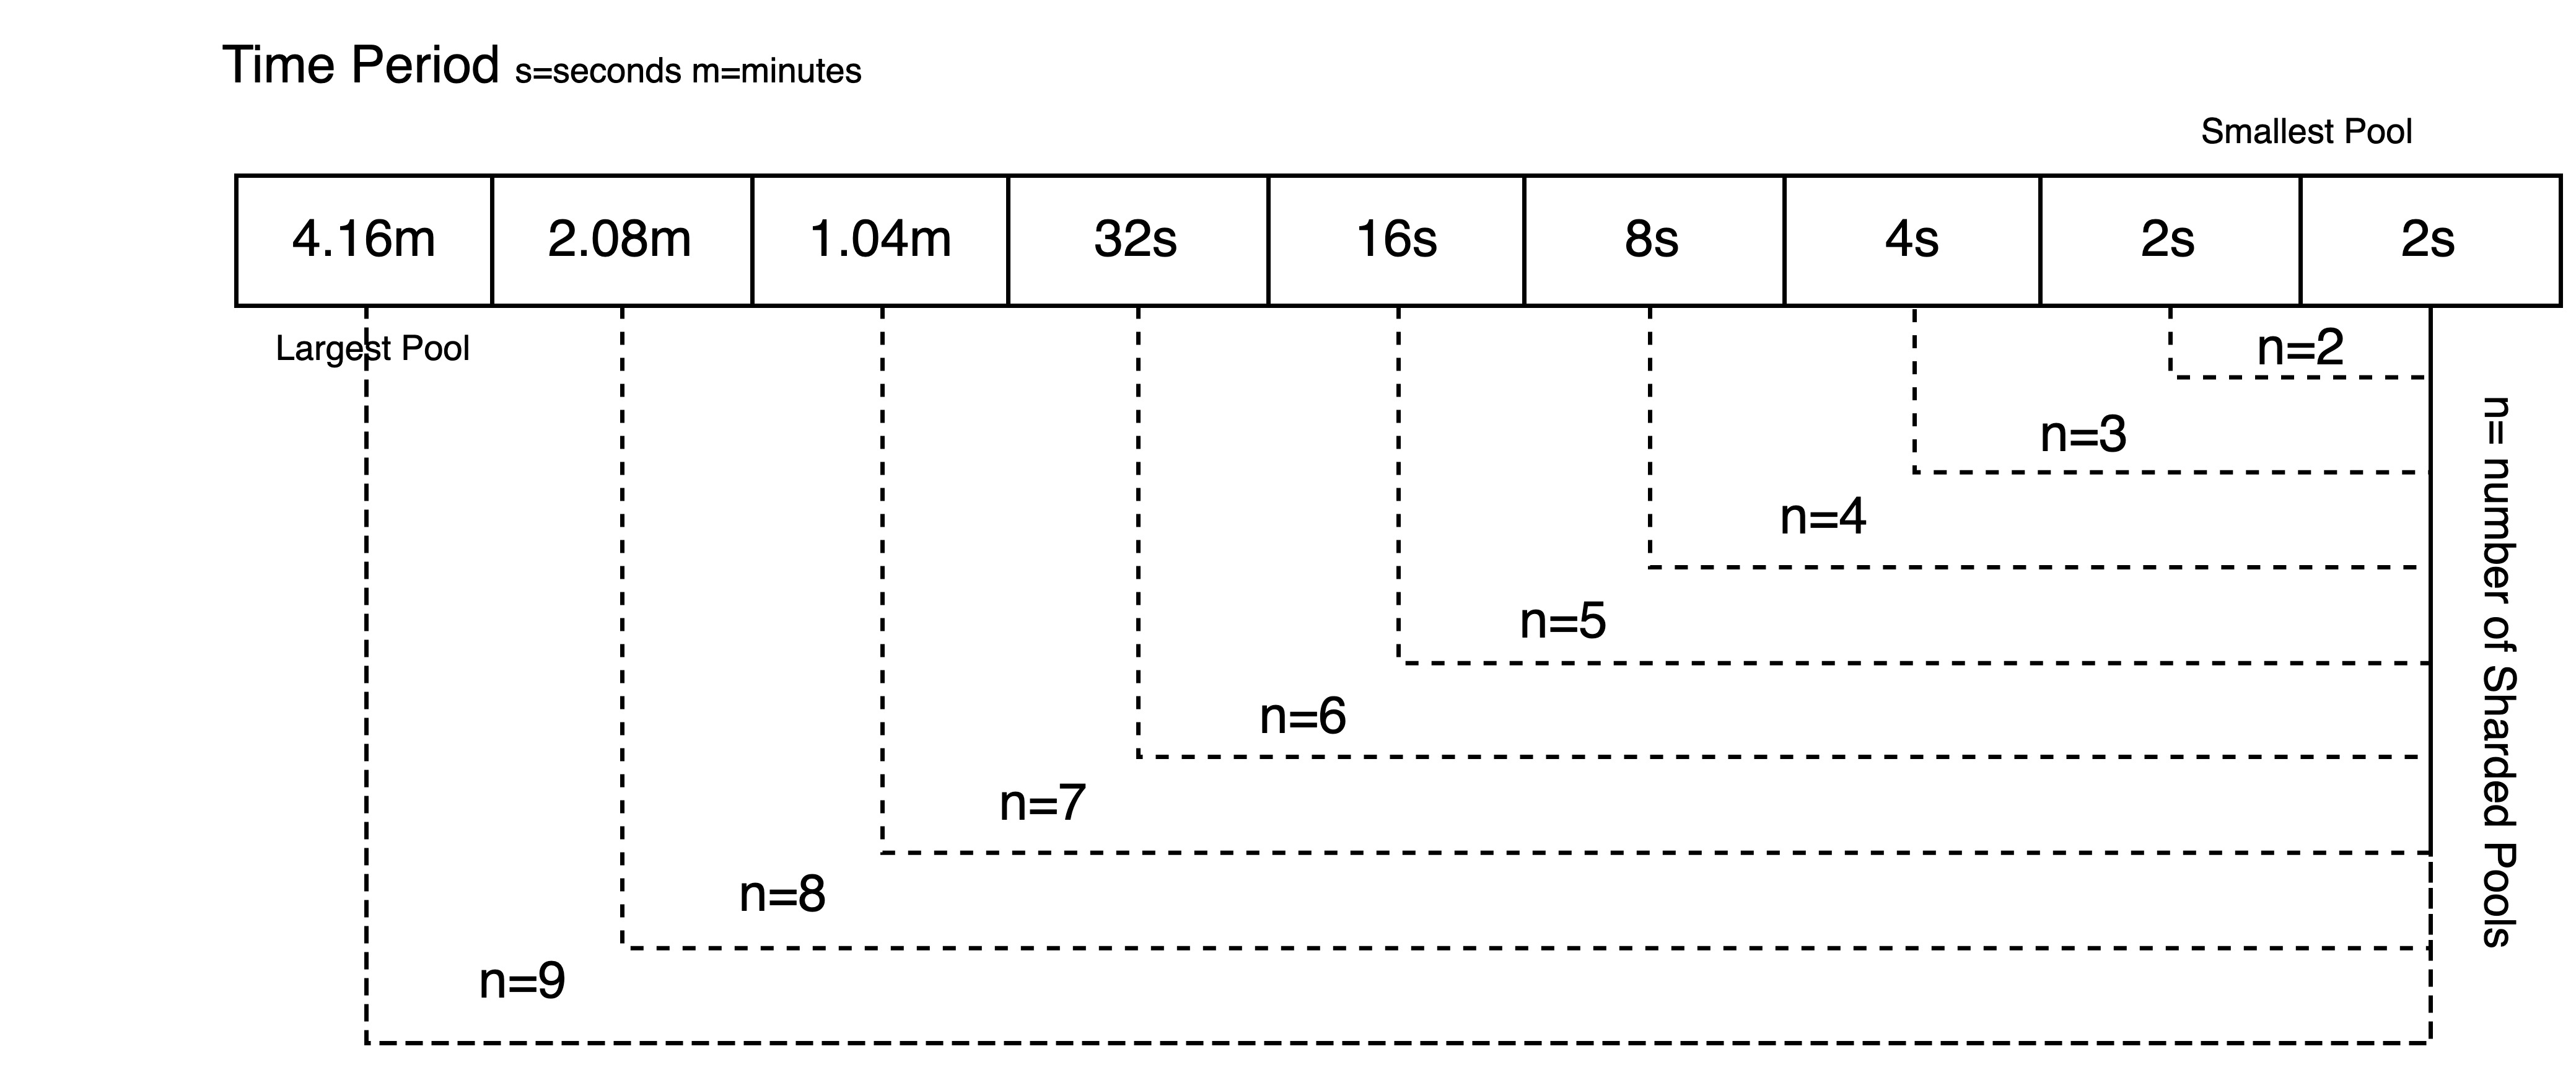
\includegraphics[width=8cm]{timeperiod-pools}
\caption{Time-period of Sharded Pools}
\end{center}
\end{figure}

For every new pool creation, the time period of all the pools will be updated accordingly. The time-period will increase by 2 times on the larger pool in descending order after every new pool is sharded i.e., 2,4,8,16,32,64,128,..n. 

\begin{figure}[H]
\begin{center}
\begin{forest}
  forked edges,
  for tree={edge+={-Latex}},
  [5 Total Pools
  	[Pool 1[50\%[16 sec]]]
  	[Pool 2[25\%[8 sec]]]
  	[Pool 3[12.5\%[4 sec]]]
  	[Pool 4[6.25\%[1 sec]]]
  	[Pool 5[6.25\%[1 sec]]]
  ]
\end{forest}
\caption{Example of Time-period of pools if number of pools (n) = 5}
\end{center}
\end{figure}

\textbf{Automated Pool Finding Algorithm}\\

Traders typically use DEX agregator softwares and applications to run complex mathematical algorithms across various DEXs to find the best possible price for a token swap with minimum impact. Most of the DEX employs a single pool for a given trading pair, where multiple DEX will have multiple pools of different algorithms and prices with price impacts. Viral implies a sharded multi-pool architecture where every pool will be priced to rebase according to the market price where the pools will have different prices. Due to the difference in prices users can able to make use of arbitrage trading by buying at low price pools or selling at higher price pools thereby running the protocol to rebase the pool by itself. \\

There are various factors a user can opt to get the best price possible. A trader can opt for two models of dex aggregator service provided in the Viral DEX, 1. Automated 2. Manual. In an automated service an algorithm is run to provide the best possible price by finding the perfect pool with the best price and instant swap support. Automated algorithm will be much faster than manual selection since it implies high efficient off-chain pool finder algorithm and can reduce man work. The user can opt for a manual method of selecting a specific pool according to his/her preference\\

\begin{figure*}
\begin{center}
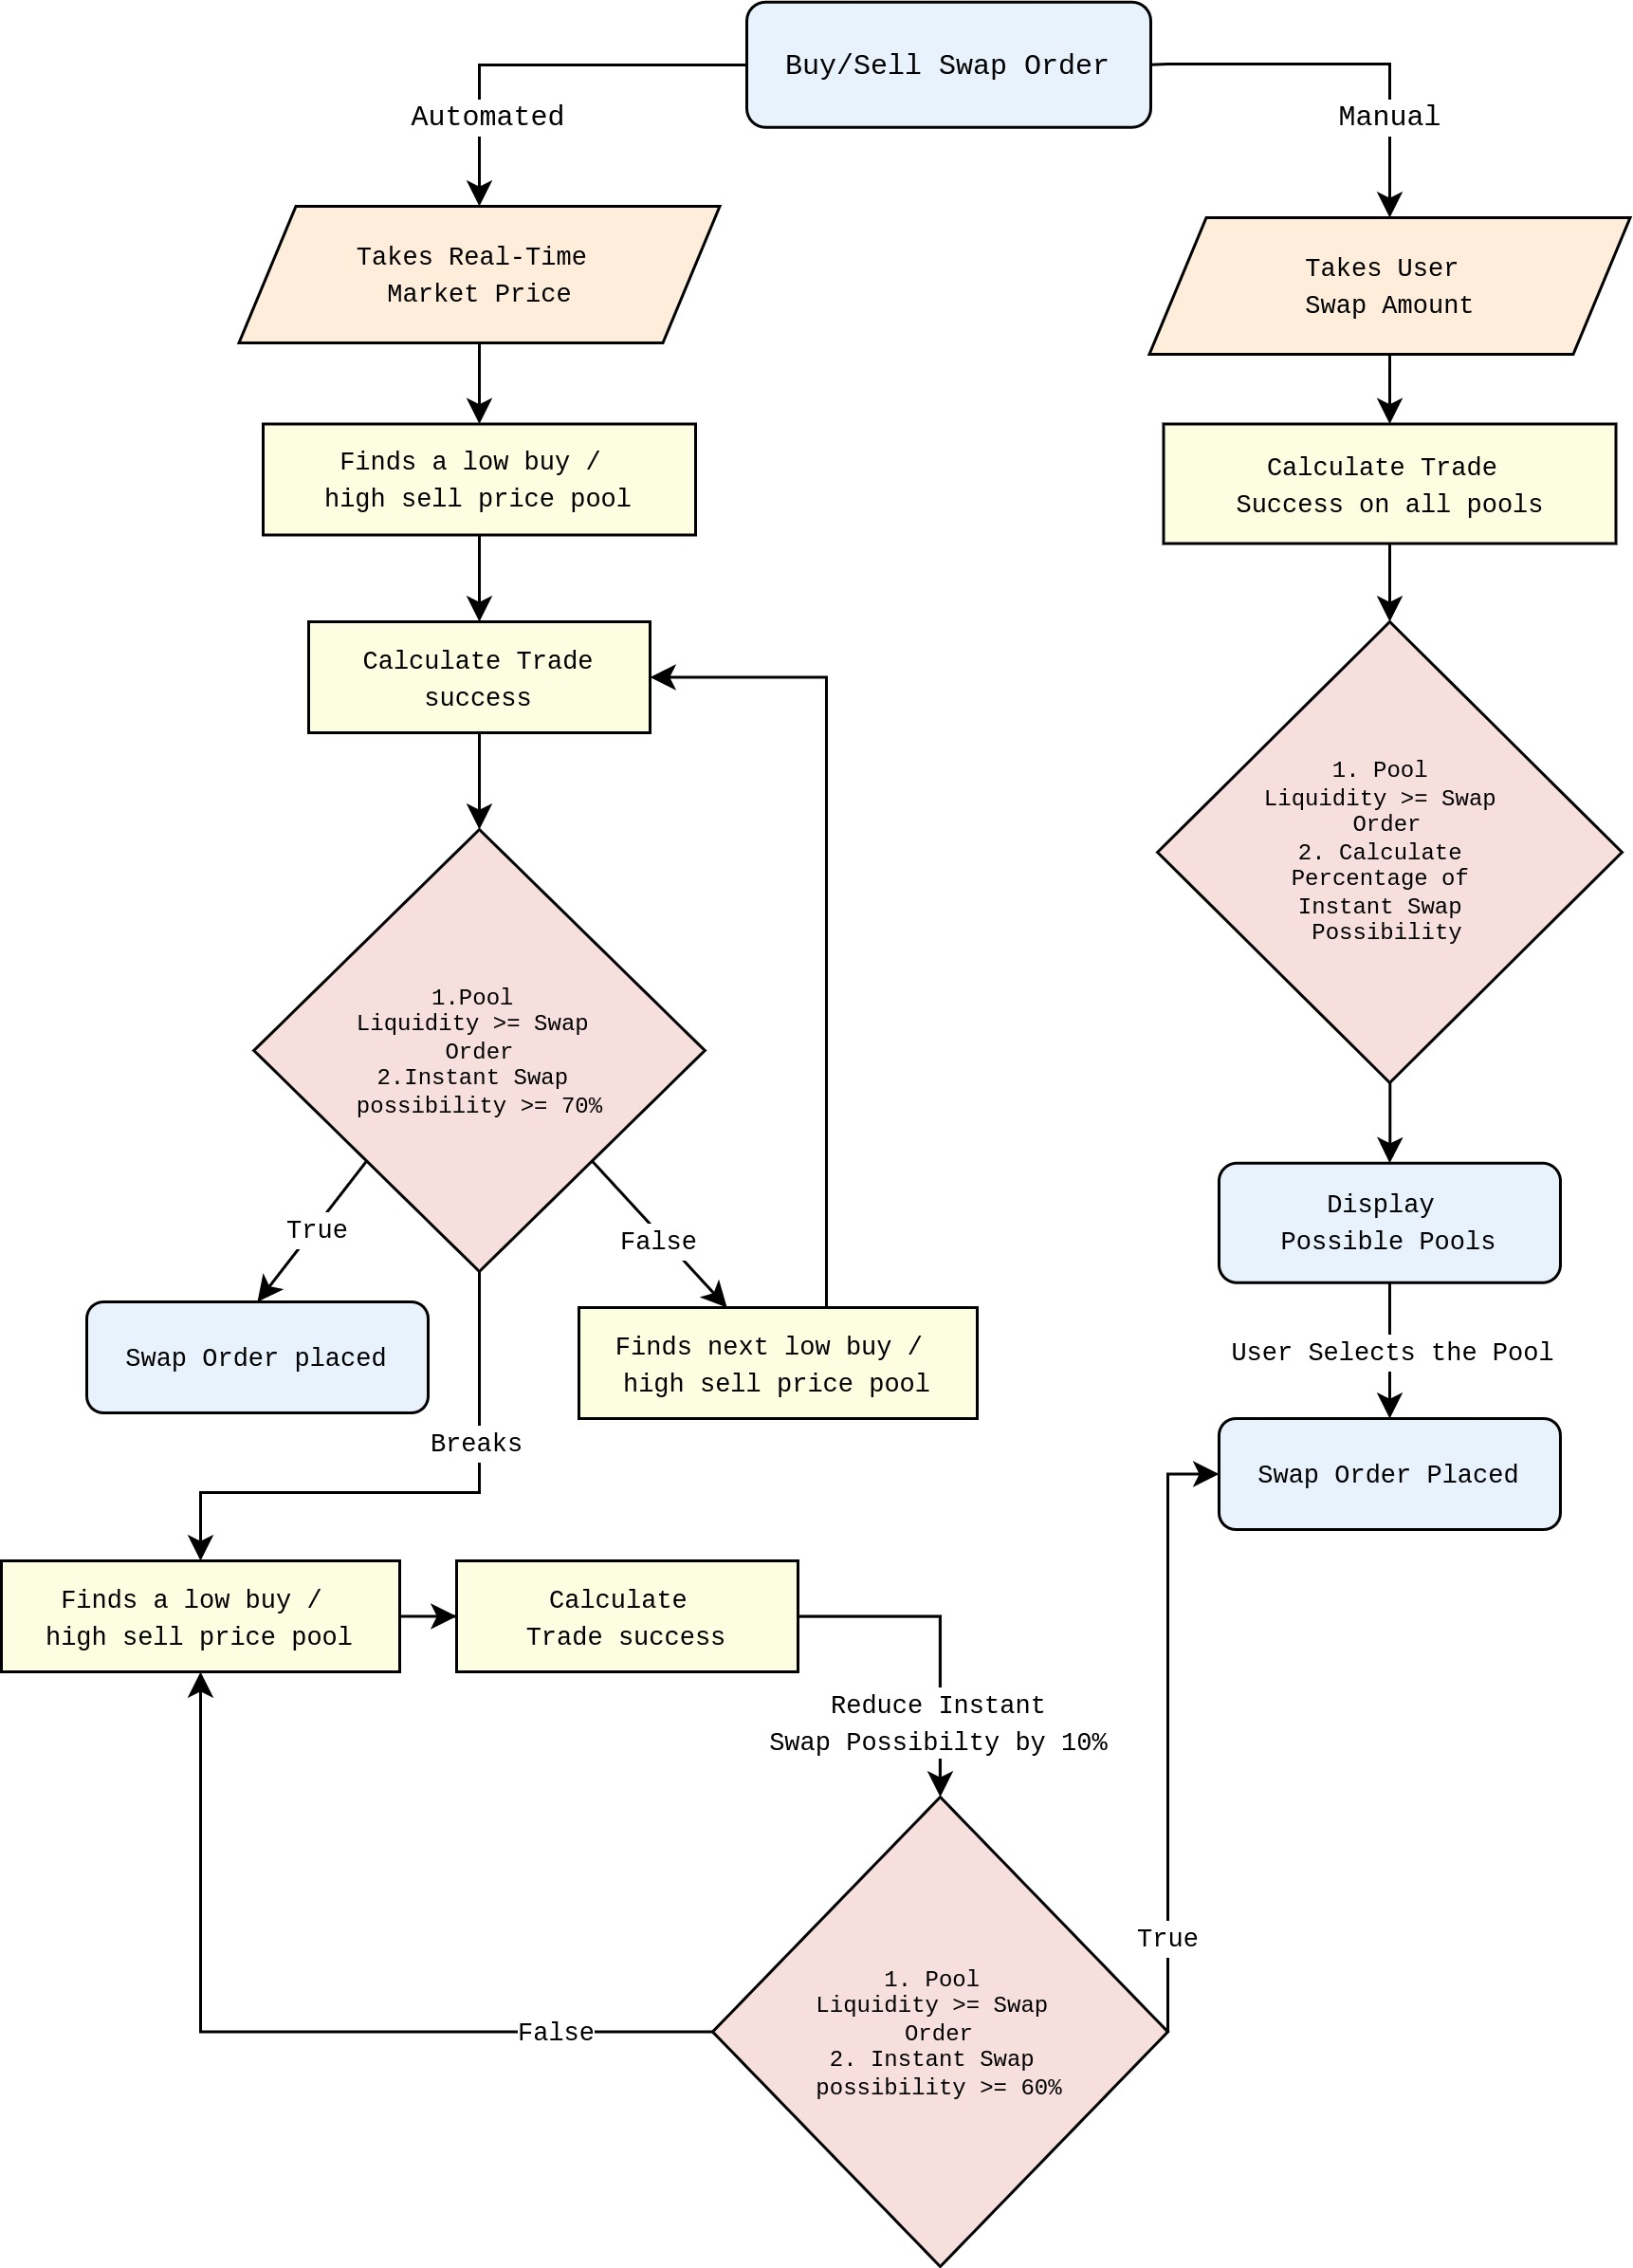
\includegraphics[width=11.5cm]{dex-algorithm}
\caption{Automated Algorithm for better price among swap orders}
\end{center}
\end{figure*}

The algorithm run as follows,
\begin{itemize}[wide, labelwidth=!, labelindent=0pt]
\item Buyers always look for lowest price and sellers always look to sell for a higher price. The algorithm will work on finding the best low/high price for buy/sell.
\item The user/trader can opt for automated or manual method for a distributed or concentrated swap order
\item The Real Time Market Price and the Swap Amount is fetched to find the low buy/ high sell price pools for maximum benefits to the traders
\item The Swap on a particular pool can only be done if the total liquidity of the pool is lesser than the swap amount. In short, the swap amount shall not exceed the total pool liquidity (since Viral implements sharded pools)
\item The instant swap possibility is calculated by analyzing the pending swap orders that can match with the oppposite orders to instantly swap the trader's order once it sent to the swap book
\item If the Instant Swap Possibility is more than 70\% on the determined pool the swap order is sent to the swap book instantly, if not the algorithm will run on the next best pool. If neither of the total available pools for a specific token is having the instant swap possibility more than 70\%, the algorithm runs again on the best pools by decreasing the percentage by 10\% i.e., 60\%, 50\%, 40\%,...
\item Executing a swap in a lower instant swap possibility pools may increase the time to sucessfully carry out a swap on the Viral DEX pools.
\item Smaller Pools may have higher instant swap possibility, but the prices reflected are realtime. Hence the prices are near to market prices offering straightforward pricing rather than low buy and high sell prices.
\end{itemize}
\[Swap\:Order \leq Pool\:Liquidity \]
The Swap Order should always be lesser than each of the sharded pools i.e., the bigger pool may receive bigger orders but will always be limited to the pool's total liquidity, a trader cannot place a 100A Token order if the pool has a total liquidity of 80A. Since Viral has sharded pools the total liquiidty of all the pools are not considered rather a single pool is considered, so the pool of the bigger pool is considered as the max i.e., the 50\% Pool.\\
\[Instant\:Swap\:Possibility \geq n = 60\%\]
\[For\:Unsuccessful\:Rounds \rightarrow n-10\%\]
The Instant Swap Possibility is determined by calculating the total pending swap orders in the particular sharded pool's swap book that can execute the newly created swap order by matching the summation of the total buy orders and sell orders. The automated pool finding algorithm will find the best pool by calculating the pool's instant swap possibility and chooses the best pool accordingly.\\

\textbf{Reserve Pools}\\

Usual DEXs employing the AMM Constant Product Maker formula requires higher liquidity in it's single bigger pools to minimize the price impacts whereas Viral DEX sharded pools requires equal liquidity to trading volume per sucessful rebase. So, a considerable liquidity per pool is better enough to rebase the pool's price to current market price of the token pairs. If a higher liquidity is provided to sharded pools where only a smaller liquidity is needed, the rebases get delayed making a spike in the price impact for the following traders making them to encounter a increased price slippage on their swap orders. Surplus of excess liquidity can be avoided in Viral DEX compared to current AMM Exchanges. Smaller sharded pools rebases much quickly in seconds where bigger pools takes couple minutes to fetch the market price and adjust the buy/sell price for the pool to rebase. To counter the effect of delayed rebases of sharded pools due to higher liquidity more than the stipulated trading volume per time period the concept of Reserve Pools are used.\\

Reserve Pools are smart contract accounts that is maintained by the trading pair's pool contract which freezes a certain portion of tokens from the liquidity pool to match the trading volume for rebasing the sharded-pools. It is exactly the same as withdrawing a certain percentage of liquidity but to a smart contract that holds the funds separately which accounts for decreasing the pool's liquidity for smoother rebases.\\

\begin{figure}[H]
\begin{center}
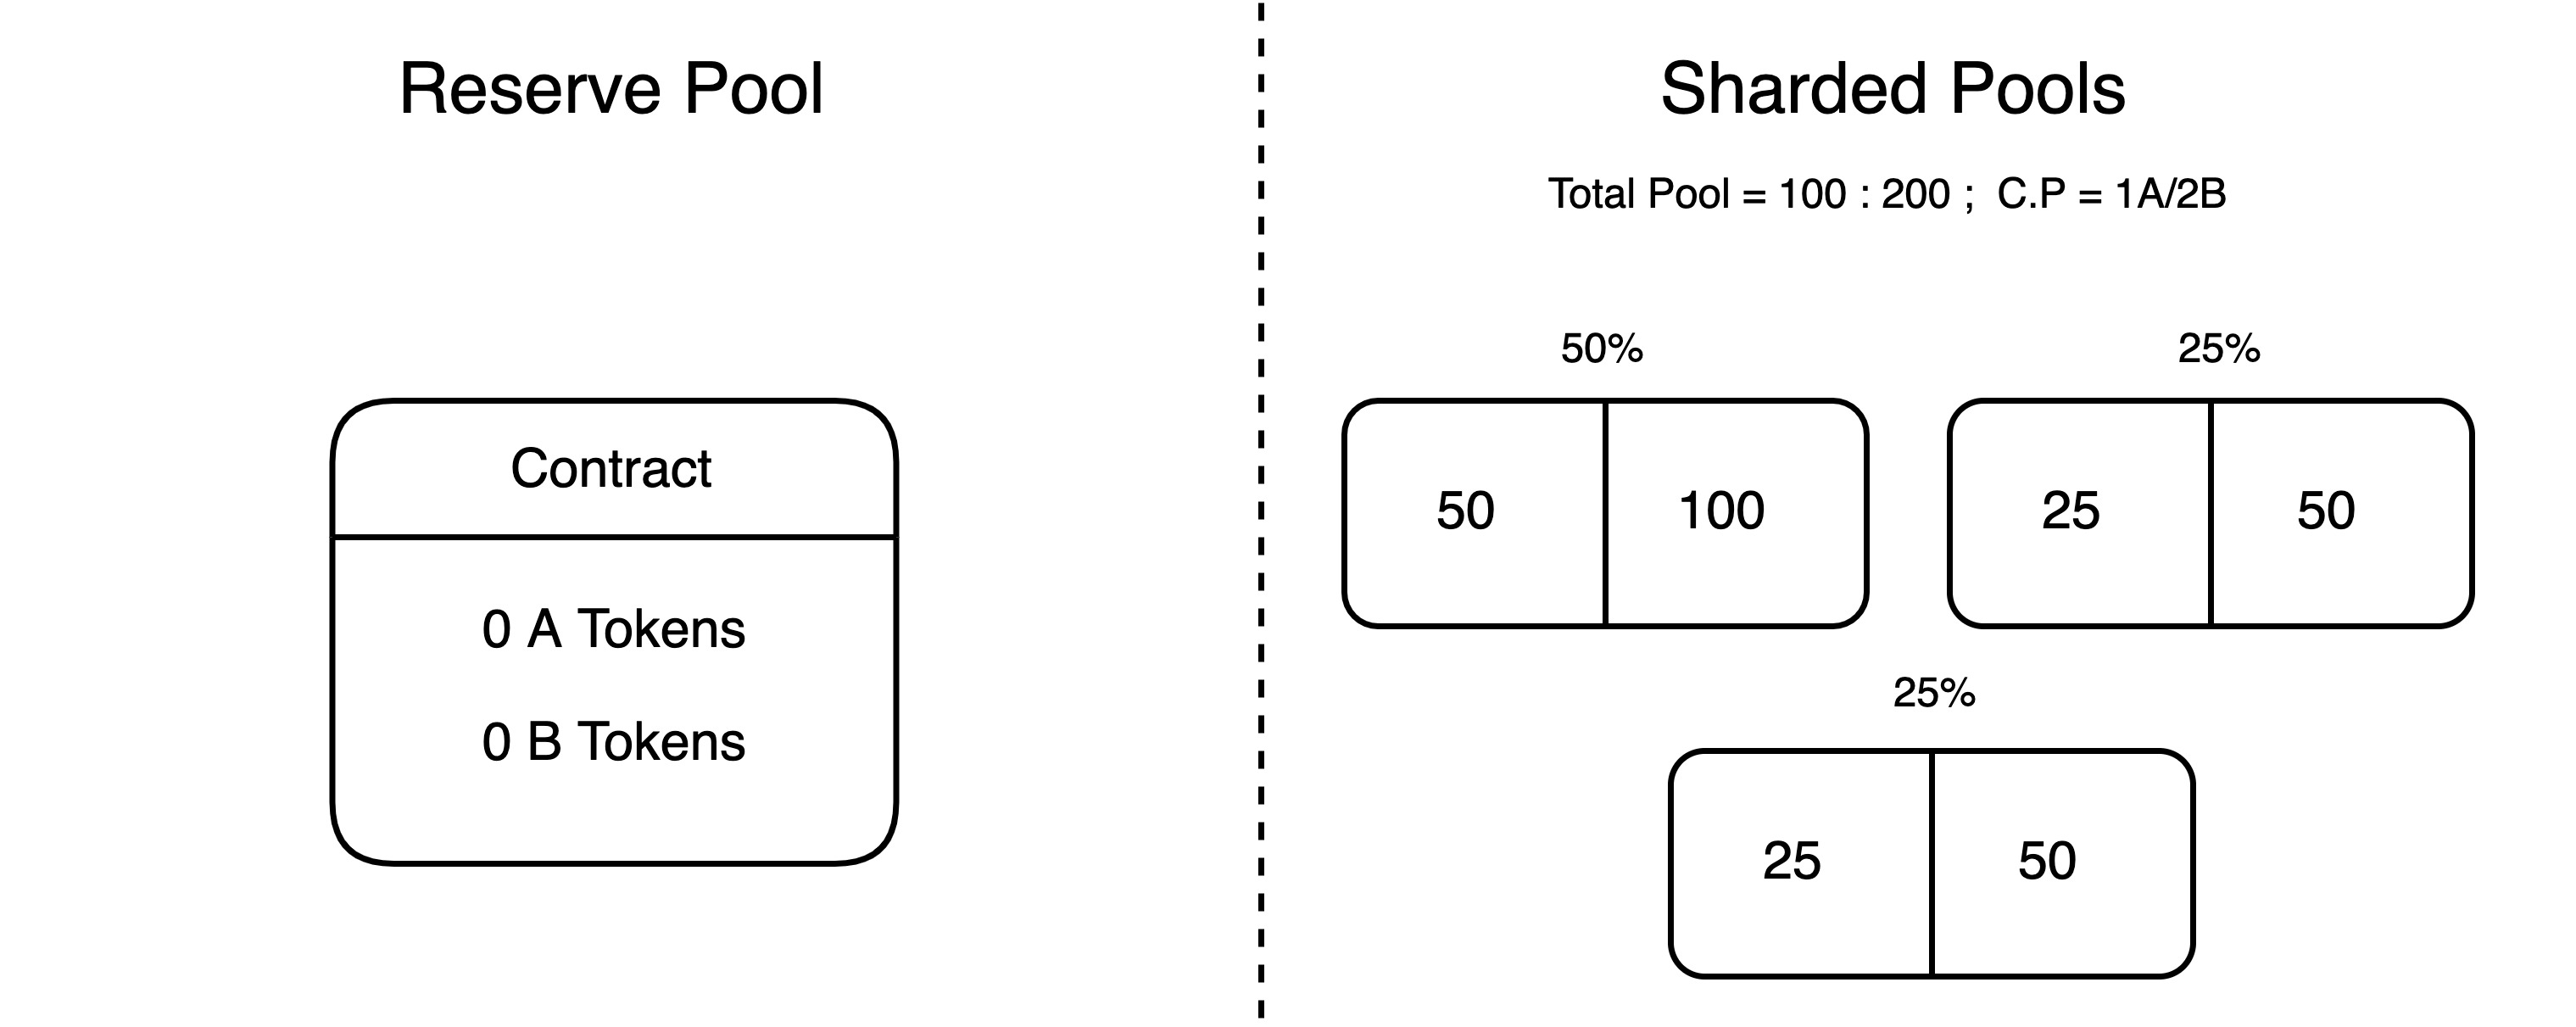
\includegraphics[width=9cm]{reserve-pool-1}
\caption{Initial Creation of Pools}
\end{center}
\end{figure}

During the initialization of the pool, the reserve pool will be set to zero where the pools will be sharded according to the pool creator's configuration where the number of dex-chains are the limit. The pools get sharded by percentage and the market price is been set by an oracle to fetch and provide buy and sell price according to the difference in current price of the pool and market price of the trading pair.\\

Liquidity gets freezed and sent to reserve pool on two occasions
\begin{enumerate}[wide, labelwidth=!, labelindent=0pt]
\item \textbf{Zero Trading Volume} : Some Pools are created for low-volume tokens that will receive low to no swap orders which then accounts for a huge price impact if the value suddenly sky-rockets making the pool to react differently to price impacts and delayed rebases
\item \textbf{Reduced Trading Volume} : Reduced trading volume gives pressure on delayed rebases on sharded pools which can be prevented by decreasing the liquidity in the pool by withdrawing it into a seperate reserve pool (similar to a wallet account but as a smart contract) 
\end{enumerate}

\begin{figure}[H]
\begin{center}
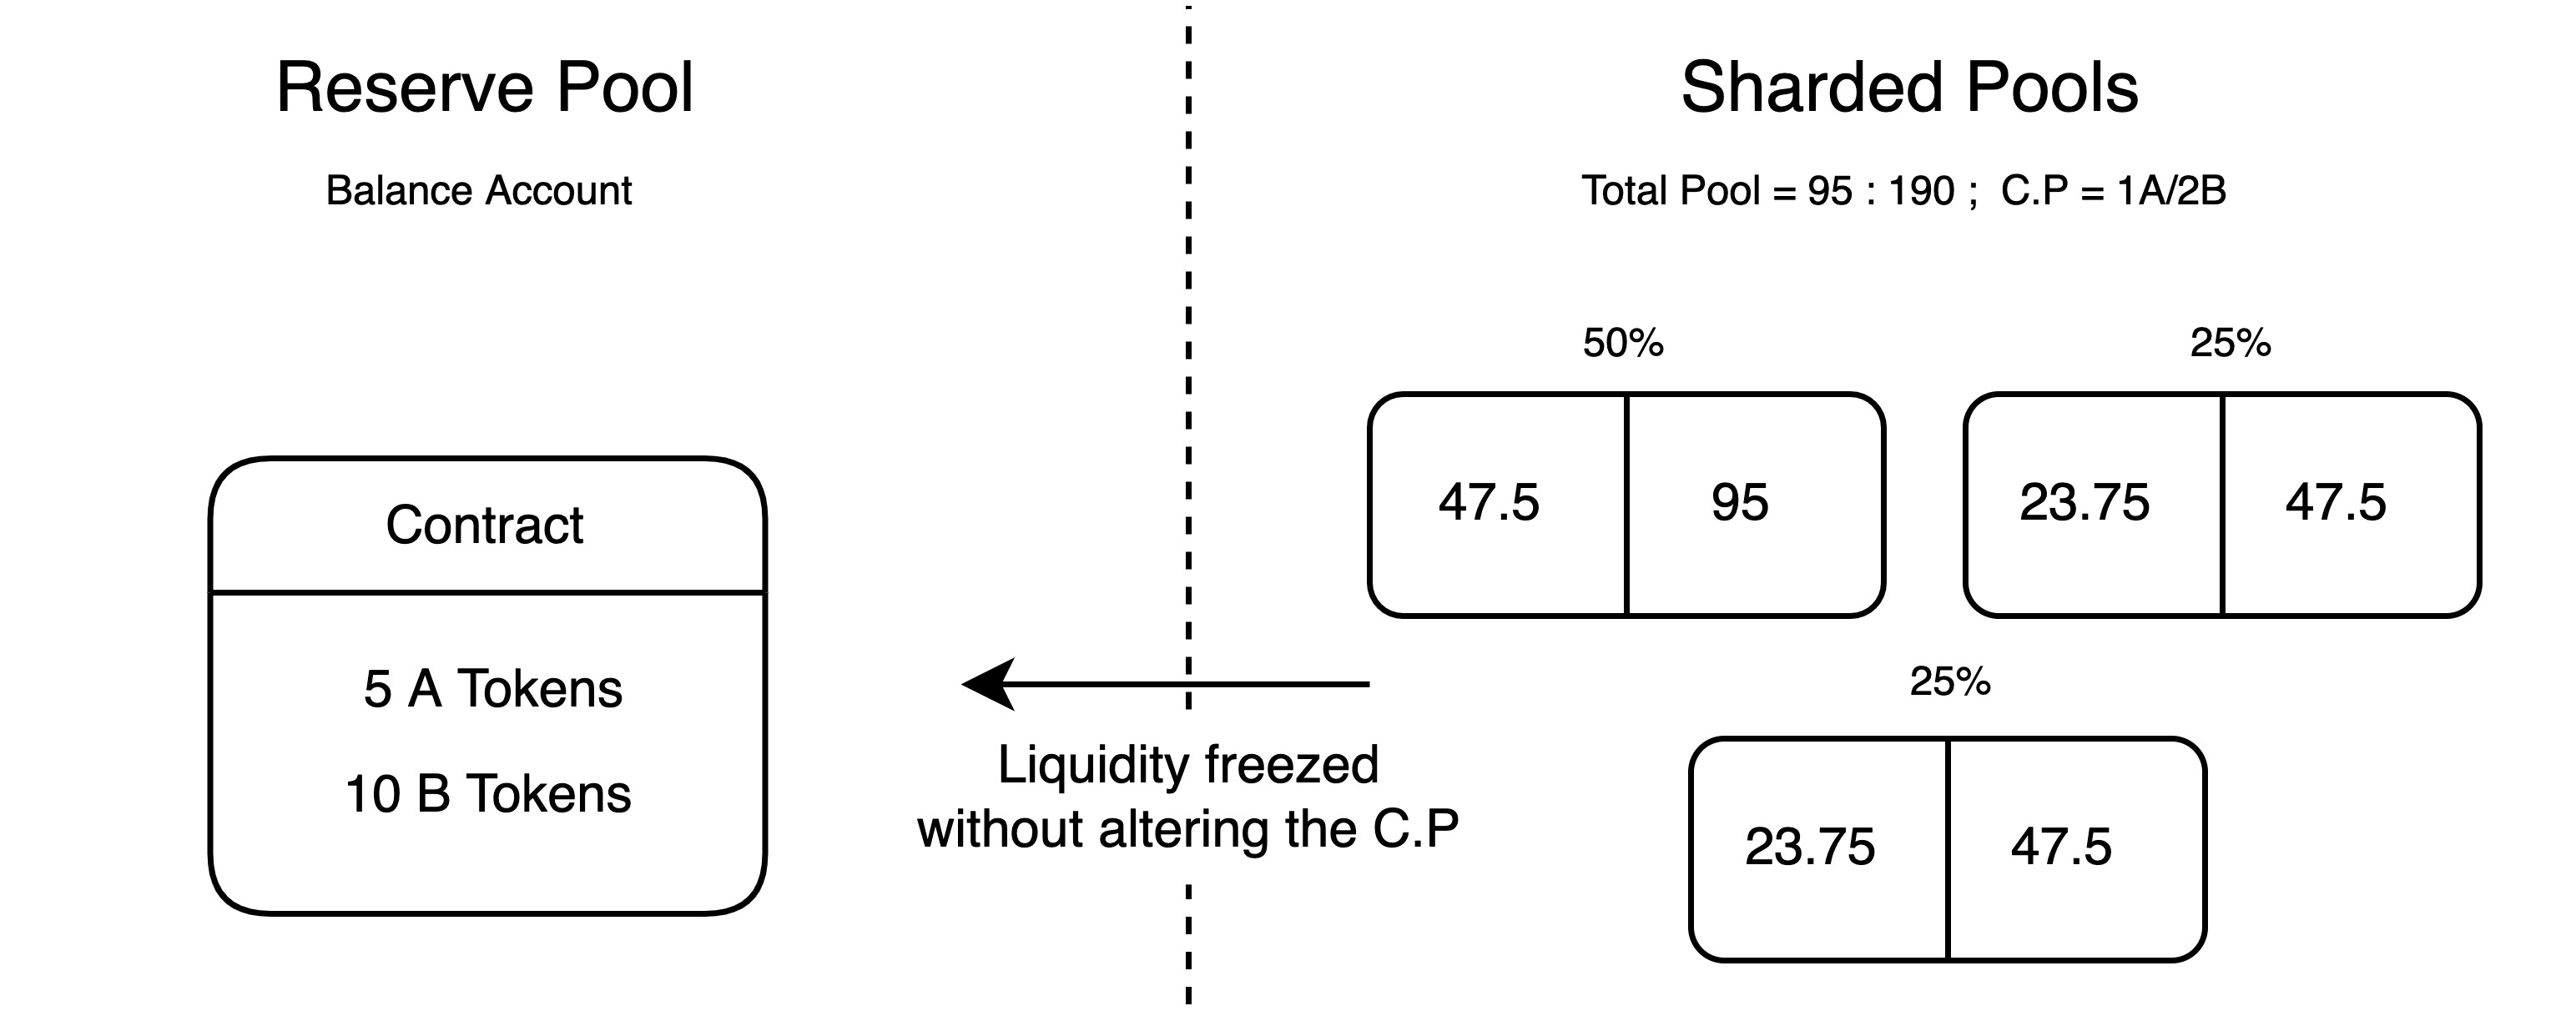
\includegraphics[width=9cm]{reserve-pool-2}
\caption{Excess Liquidity Freezing}
\end{center}
\end{figure}

Pools will withdraw tokens in to its reserve pool on request. The withdrawal ratio will be equal to the Current Price ratio of the current pool not affecting the pool's price. When each pool has different ratio of tokens (possible scenario due to Time Average Market Prices- TAMP) an equal percentage from all the pools shall be withdrawn to maintain the micro-pool architecture. In simple words from each pools the tokens will be withdrawn at a same percentage and sent to it's reserve pool to decrease the liquidity for better rebases.\\


\textbf{Limit Orders}\\

Viral uses an off-chain swap book that matches the summation of primary coin/secondary coin buy and sell orders to execute a swap in the Viral DEX Liquidity Pools that sets a pricing strategy in accordance with rebasing the pool's liquidity to fetched real-time market price of the trading pair. Since it incorporates an off-chain swap book without executing the swap instantly like other DEXs the makers can benefit the features of limit orders and therby making the trading pair liquid in nature. Users can make use of limit orders to buy and sell when the maket reaches a certain price. The limit order gets placed in a seperate book that will run automated pool find algorithm and determines when a pool reaches a limit price and passes the order to the swap book and executes the swap instantly.\\


\textbf{Fee Structure}\\

Intro to Fees, Fee Structure of other DEXs\\
Type of tokens and Fees structure\\
Fees allocation for LPs and Reward Pool\\
Examples\\


Viral DEX subtracts a swap fee on every swap order executed. There are two types of fee leaved according to trading pairs nature. A 0.2\% fee will be leaved on normal pairs and a 0.02\% fee will be leaved for stable-coin pairs. These DEX fees are excluding wallet transfer fees which will be leaved separately. These fees will be added into a separate pool where the liquidity providers can collect while withdrawing their staked tokens. 70\% of total DEX fees collected with be allocated to liquidity providers where the rest 30\% will be sent to Viral's global revenue pool.\\

\begin{figure}[H]
\begin{center}
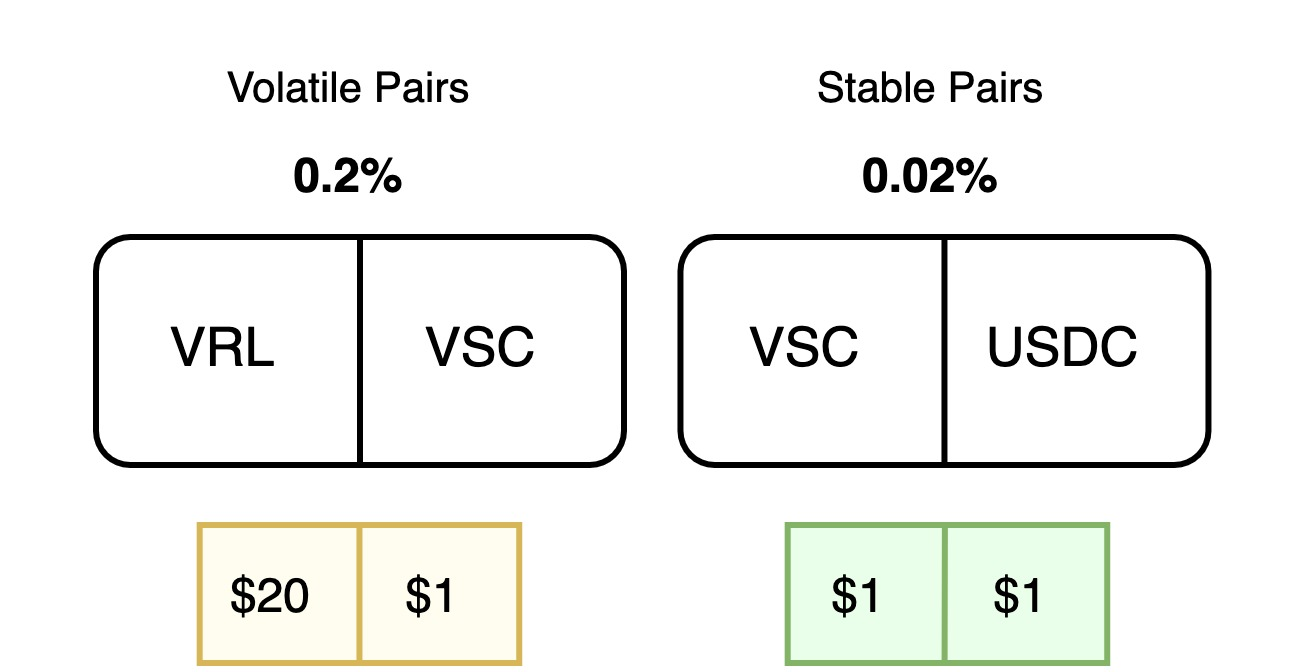
\includegraphics[width=7cm]{dex-fee}
\caption{Fee Structure}
\end{center}
\end{figure}
\[Normal\:Pair\:Swap\:Fee=Swap\:Amount \times  0.2\%\]
\[Stable\:Pair\:Swap\:Fee=Swap\:Amount \times  0.02\%\]
\[Transfer\:Fee=After\:Swap\:Fee\:Rate \times  Transfer\:Fee\]
\textit{For Example} 
(Fee Type : Normal Pair) \\
Total Swap amount = $500$\\
DEX Fee : $500 \times  0.2\% = 1$ \\
Transfer Fee= $((500)-(500 \times  0.2\%)) \times  0.05\% = 0.2495$ \\
Final = $498.7505$\\

(Fee Type : Stable Pair) \\
Total Swap amount = $500$\\
DEX Fee : $500 \times  0.02\% = 0.1$ \\
Transfer Fee= $((500)-(500 \times  0.2\%)) \times  0.05\% = 0.24995$ \\
Final = $499.65005$\\
 
 
\textbf{Liquidity Providers}\\

\begin{figure*}
\begin{center}
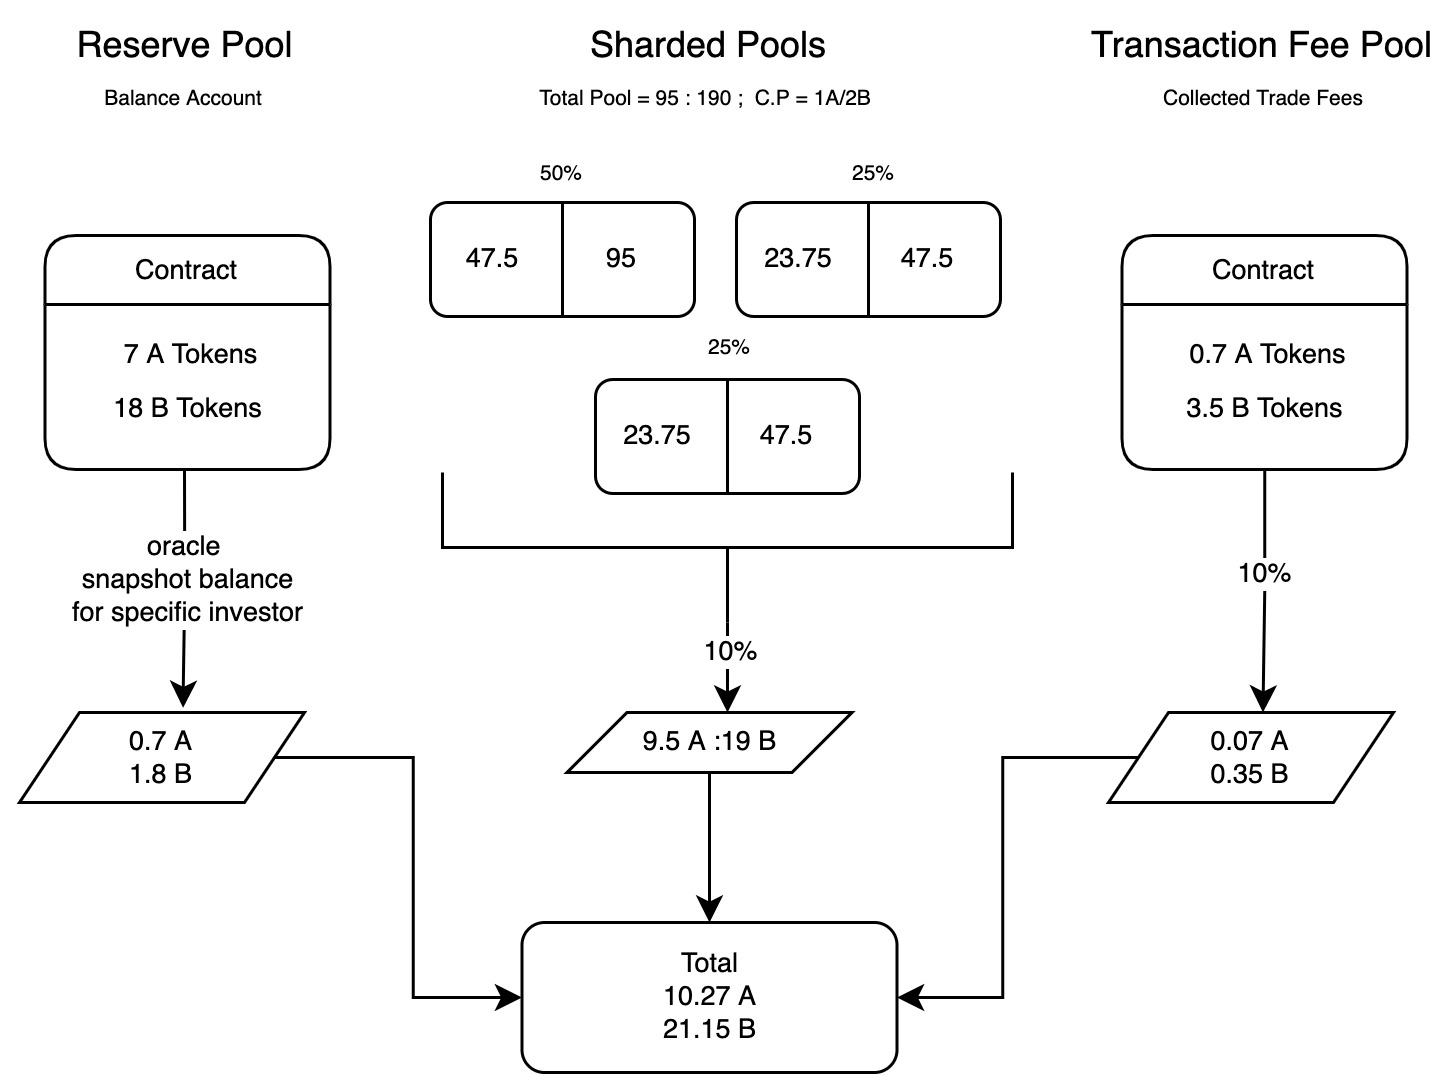
\includegraphics[width=13cm]{reserve-pool-4}
\caption{Liquidity Provider withdrawal of Funds from all reserves}
\end{center}
\end{figure*}


Liquidity providers are investors who stake their cryptocurrency tokens on DEXs to earn transaction fees, often referred to as liquidity mining or market making. Viral Liquidity providers earn transaction fees for their staked tokens in the Viral Smart Chains protocol. The transaction fees are distributed proportionally to all the liquidity providers in the pool according to their percentage of investment. Sine Viral implies micro-pool architecture the liquidity is divided among several micro-pool running blockchains while depositing and withdrawing funds.\\


\textit{For Example}\\

Pool = 1600 : 4,992 LP provides tokens 20 : 62.4 equally to the pool. No.of Micro-Pools = 4\\

\begin{figure}[H]
\begin{center}
\begin{forest}
  forked edges,
  for tree={edge+={-Latex}},
  [20 : 62.4
    [50\%
        [10 : 31.2]
    ]
   [25\%
        [5 : 7.8]
    ]
    [12.5\%
        [2.5 : 3.9]
    ]
    [12.5\%
        [2.5 : 3.9]
    ]
  ]
\end{forest}
\caption{Division of LP funds to micro-pools}
\end{center}
\end{figure}

When it comes to withdrawing funds from main pool and transaction fee pool the funds will be distributed according to his percentage the LP holds in the current pool i.e If a LP provide 10:20 in a 100:200 Pool, the LP holds 10\% of the pool's liquidity. Current AMM models deploy the same concept of withdrawal of percentage investment in a pool of many investors funds. Withdrawing funds from the reserve pool is determined by off-chain oracle's zero-knowledge-snapshots of rebases that contains balances of each investors funds updated every snapshot (here snapshot represent every iteration of freezing user's funds). \\

Snapshots
\begin{enumerate}[wide, labelwidth=!, labelindent=0pt]
\item VNS-id : Token A Balance : Token B Balance
\item example : 10 : 50
\end{enumerate}

Upon withdrawal the investor deducts his balance from the reserve pool accordingly along with main pool funds and transaction fee pool funds. The Reserve pool can be determined as a wallet smart contract that hold's the LP funds which are not required for the main pool. When a small percentage of LP's invest their tokens into a restricted liquidity pool, trnsaction fee may distributed among a small group of LP's which can provide a better ROI compared to current AMM pools.


\textbf{Benefits of Viral DEX}
\begin{enumerate}[wide, labelwidth=!, labelindent=0pt]
\item \textbf{Affordable Fees} : Competitive low-priced fees 0.2\% for Normal pairs and 0.02\% for Stable pairs.
\item \textbf{Free from Price Impacts} : Price impacts are eliminated since to execute a swap order both the buyer and seller orders should be matched and swapped at once as a single order which eliminates the price impacts.
\item \textbf{Real-Time Market Price Pool Rates} : Constant Product Maker is not used rather the pool will determine the buy \^ sell price by finding a difference between the current pool price by it's ratio and the market price of the trading pair to rebase the pool always to the market price.
\item \textbf{Faster Swaps} : Sharded Micro-pools deployed on separate chains brings parallel executions of faster swaps .
\item \textbf{Reduced Human-work} : Automated Pool Finding Algorithm shall find the best pool by determining the lowest buy / highest sell price and instant swap possibility by calculating how much liquid a particular pool's swap book orders are.
\item \textbf{Multi-Layer Security} : The Viral Multi-Chain Architecture  offers an immutable state anchoring of each chain's global state to the Tangle (DAG) for additional security.
\item \textbf{Advanced Trading} : Since Viral employs a strategy to receive all the orders on a off-chain swap book, it can receive limit orders for institutional and retail market makers who would like to trade on DEXs.
\item \textbf{Less Volatility} : Real-Time Market Prices are taken in account for the pool rebases that makes the pool less volatile compared to current AMMs that have huge volatility upon larger orders.
\item \textbf{Congestion-Free DEX} : Congestion is eliminated by incorporating micro-pools where larger pools for larger orders and smaller pools for smaller orders.
\item \textbf{Multi-Order Matching} : Comparing to Order book exchanges which matches a buyer and seller, where Viral DEX matches multiple orders who can execute an order in a single swap.
\item \textbf{Higher Yields for LPs} : Unlike current AMMs that require larger pools to become stable without volatile effects, Viral requires only a liited amount of Liquidity equal to the trading volume, which can provide a smaller group of LP's maximum yields.
\end{enumerate}

\section{\textbf{Viral Fiat-Exchange}}

Centralized exchanges (CEXs) are a type of cryptocurrency exchange that is operated by a company that owns it in a centralized manner. Centralized exchanges most commonly facilitate trades between users by maintaining an order book: a collection of buy and sell orders posted by individual traders. CEX users do not actually exchange crypto or fiat currencies with each other. Instead, when they deposit their funds onto an exchange, the latter takes over the custody of the crypto assets and issues a corresponding amount to the buyer and seller. Users store their crypto assets on the exchange. Since the private key's ownership rests with the exchange, there is a risk of total loss should the exchange be compromised (Not your Keys, not your Coins). Cases of this kind are rare but historically have already occurred with losses in millions. CEX exchanges are under the control of regulators, third-party providers, and legal regulations. To prevent money laundering, operators are required to collect extensive data about their customers (KYC). This regularity is contrary to the basic idea of cryptocurrencies.\\

\textbf{Common Insecurities Investors have on Centralized Exchanges}\\

Ironically, many of the same factors that contribute to the advantages of a centralized exchange also contribute to the disadvantages.
\begin{enumerate}[wide, labelwidth=!, labelindent=0pt]
\item \textbf{Custody}: Entrusting an exchange with your private keys means you don’t fully control your own money.

\item \textbf{Security}: Because they hold a large number of assets, centralized exchanges are a prime target for bad actors. The most notorious exchange hacks were aimed at centralized exchanges (e.g., Coincheck, Mt. Gox, BitGrail, NiceHash, and Bitfinex).

\item \textbf{Manipulation}: Several centralized exchanges have been accused of manipulating their opaque nature and conducting insider trading, fake volume, and price manipulation.
\end{enumerate}

\textbf{Security Threats}\\

As the security threats continues, there's currently no effective solution for a non-custodial fiat-crypto exchange. At any instance if a probable propaganda is proposed the primary user aquisition strategy of those solutions is to target the current users of popularly running cryptoexchanges which is a very long and narrow way to bring in users for the platform. Viral has a first mover advantage for such a non-custodial way of buying cryptocurrencies using fiat-currencies since it's application offers end to end solution on all aspects on the de-fi wave, user's are prompted to use it's services while using the application. This has a significance effect in acquiring users for an in-built crypto buying facility for users to trade in their fiat money. For one such of an exchange where it's users derived from a social media will impact the crypto adoption and also reassures the year-long threat of losing user's funds to potential hackers.\\

\textbf{Intro to Viral-FEX}\\

Decentralization refers to freedom and ownership. A centralized exchange restricts the ownership by being a custody to user's funds by maintaining the private keys on their central server. There is only two aspects a CEX will carry out: Buying and Selling. While both fiat and crypto funds is being held in custody, the Fiat Funds is securely holded (due to it's reversal mechanism), whereas the Crypto Funds are always open for attacks and cannot be reverted back nor easy to track the route of transactions to an individual after a breach. While Popular CEXs are tackling these breaches using secured cryptographic encryptions, firewalls, etc there is always a possibilty for a penetration expert to steal the funds. Viral is offering a non-custodial crypto buying solution by supplying fiat-pegged-tokens and exchanging via Viral DEX.\\

\textbf{Basic Structure}\\

Viral Buy/Sell Exchange works differently from centralized exchanges. In current CEXs when user deposits his fiat funds, the funds will get deposited into the exchange's traditional banking account from where the user gets his fiat balance updated with a total figure he would have deposited. CEXs tracks user's fiat balances in a centralized manner and directly updates the database tables of each user after making successful trades. The update in fiat balances are done through centralized systems which is not transparent and needs to be trusted. This effectively comes to the usage of Fiat-backed-crypto tokens such as USDC, USDT, TrueUSD which holds equally backed fiat amount in reserves and thereby minting new tokens for user in which the is pegged 1:1 to a government backed fiat currency .i.e., typically US Dollar.\\

Nowadays most users prefer to buy USDC and later use those tokens in various DeFi applications. The emergence of fiat backed tokens have paved a way of tokenizing fiat coins. As Viral's vision to bring rapid adoption to tokenized economy we provide our users to buy Viral Coins from fiat currencies by adopting fiat-tokenization strategy and swap books of Viral DEX for exchanging tokenized fiat to Viral Coin and vice versa.\\

In simple words while today's crypto exchanges updates the fiat balance when users deposit their fiat currencies i.e., dollar, euro, yen, rupee into the exchange, while Viral Exchange provides users who deposit an equivalent amount of special Fiat-Tagged tokens (Eg; USD, INR, EUR - all as crypto tokens) into their current non-custodial Viral wallet that can be referred as fiat balance from which users can trade in for Viral Coins. While buying and selling Viral Coins the users will be using their Fiat-Tagged Tokens to facilitate trades using a decentralized Swap Books Exchange between white-listed addresses\\

A solution which combines decentralized solutions is a better, safer and cheaper alternative to current custody model exchanges. Since deposit and withdrawal of fiat funds are subject to regulatory compliance some of the process such as KYC, AML will be required for users. Some of the benefits compared to current exchanges are
\begin{enumerate}[wide, labelwidth=!, labelindent=0pt]
\item \textbf{Security of Funds}: Stored in Non-Custodial Wallet
\item \textbf{Decentralized Exchange}: Atomic Swaps happen on-chain and orderbook will be maintained off-chain
\item \textbf{User Owned Private Key}: Hot Wallets where user owns his/her private key and has complete ownership of deposits
\end{enumerate}

\textbf{User Registration}\\

\begin{figure}[H]
\begin{center}
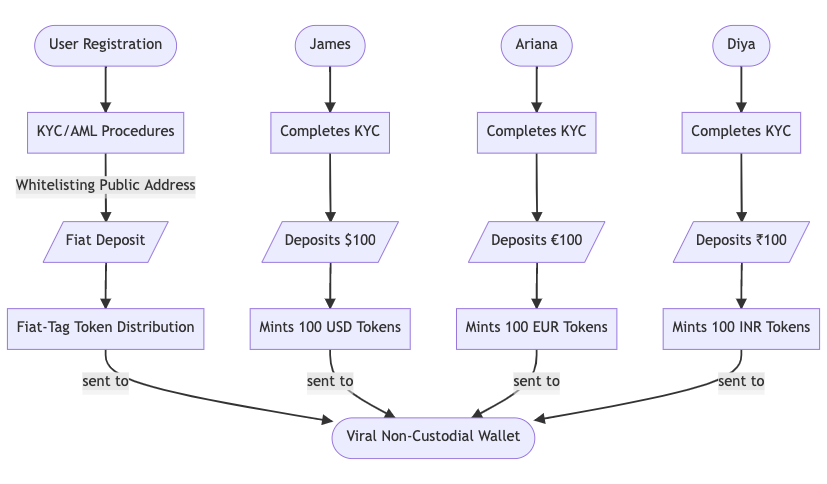
\includegraphics[width=8cm]{user-deposit}\\
\caption{User Deposit and Fiat-Tag Token Distribution}
\end{center}
\end{figure}


\begin{comment}%mermaid
graph TB
    
    A([User Registration])
    C[KYC/AML Procedures]
    D[/Fiat Deposit/]
    E[Fiat-Tag Token Distribution]
    A-->C--Whitelisting Public Address-->D-->E

    F([James])
    G[Completes KYC]
    J[/Deposits \$100/]
    K[Mints 100 USD Tokens]
    F-->G-->J-->K

    L([Ariana])
    M[Completes KYC]
    N[/"Deposits €100"/]
    O[Mints 100 EUR Tokens]
    L-->M-->N-->O

    Q([Diya])
    R[Completes KYC]
    S[/"Deposits ₹100"/]
    T[Mints 100 INR Tokens]
    Q-->R-->S-->T


    P([Viral Non-Custodial Wallet])
    E & K & O & T--sent to-->P
\end{comment}

While Viral application doesn't require any user information, ViralFEX will require user's information such as email, phone verification, etc and also will require Know-Your-Customer (KYC) and Anti-Money-laundering (AML) policies for regulatory purposes. After the registration completes the user's viral wallet username (VNS) will get linked automatically to get white-listed for the exchange (since it's decentralized) and securely drop in fiat-tag tokens directly into the user's VNS-linked Viral Smart Chain wallet address. 


\begin{figure}[H]
\begin{center}
\begin{forest}
  forked edges,
  for tree={edge+={-Latex}},
	[Fetches Viral Username
		[Whitelists-username
			[$username$ returns address
				[$0x71C7656EC7ab88b098defB751B7401B5f6d8976F$]
			]		
		]	
	]
\end{forest}
\end{center}
\end{figure}

\textbf{Fee Structure}\\
Since Viral-FEX deals with only deposit \& withdrawal where the exchanging mechanism depends on swap books and ViralDEX Pools the fees on  Viral Semi-CEX is considerably low compared to other popular centralized exchanges. Viral takes fees based on deposit, withdrawal and trade. These fees doesn't include the network fees paid to the Viral Smart Chain which will be included seperately. Since Viral Smart Chain doesn't take gas fees and takes a very minute amount of base fee \$0.0005 and a transfer fee of 0.05\% it will not affect the users trades. The exchange fees are listed below\\

\textbf{Deposit fees}
\begin{enumerate}[wide, labelwidth=!, labelindent=0pt]
\item \textbf{Deposit Fee}: Fized 0.1\% excluding credit/debit card or bank transfer fee
\item \textbf{Mint Fee}: Fee charged for minting new fiat-tag tokens .i.e., typically \$0.0005
\end{enumerate}

\textbf{Trade Fee}\\
The trade fee is fixed to 0.2\% for Viral Coin- Fiat Pairs and 0.02\% for Viral Stable Coin - Fiat Pairs. These fees will be allocated to 70\% Liquidity Providers and 30\% Viral Global Revenue Pool\\

\textbf{Withdrawal Fee}
\begin{enumerate}[wide, labelwidth=!, labelindent=0pt]
\item \textbf{Withdrawal Fee}: Fixed 0.1\% excluding credit/debit card or bank transfer fee
\item \textbf{Burn Fee}: Fee charged for burning fiat-tag tokens .i.e., typically \$0.0005
\end{enumerate}


\textbf{Fiat-Tag Token Supply}\\
Fiat-Tag Tokens are limited tokens that is minted and supplied to FEX users after depositing fiat money i.e., USD, EUR, INR, etc to their exchange accounts. The utility of these tokens is only limited for exchanging purposes inside the viral application. The tokens are classified by listed fiat currencies from which users are allowed to exchange e.g., If Euro can be deposited to Viral FEX account, EUR Tokens will be generated and sent. The supply of tokens are elastic in nature while minting and burning while depositing and withdrawing fiat funds. KYC users addresses will be white-listed for transacting fiat-tag tokens to eliminate spam and usage of tokens by a non-kyc users.\\

\begin{figure*}
\begin{center}
\begin{tabular}{ |p{3cm}||p{3cm}|p{3cm}|p{3cm}|  }
 \hline
 \multicolumn{4}{|c|}{Fiat-Tag Tokens} \\
 \hline
 Fiat Currency & Fiat-Symbol & Region & Tag-Token\\
 \hline
 US Dollar &\$ & United States & USD\\
 Euro & €  & Europe  & EUR\\
 Japanese Yen &¥ & Japan & YEN\\
 Pound Sterling &£ & Britain & GBP\\
 South Korean Won &₩   & South Korea & KRW\\
 Indian Rupee &\rupee & India  & INR\\
 Canadian Dollar &\$ & Canada  & CAD\\
 \hline
\end{tabular}
\caption{ViralFEX Fiat Tag Tokens}
\end{center}
\end{figure*}


\textbf{Minting Tag-Tokens / Fiat Deposit}\\
Fiat-Tag Tokens will be minted upon a KYC user's deposit of funds to allocated fiat-holding reserve bank. User's funds are holded by custodian banks fiat holding accounts. Viral allows partnership of centralized banks for holding, minting and distributing tokens to Viral-FEX users for a decentralized approach of exchanging crypto for fiat. Minting Tag-Tokens are carried out by the  custodians on behalf of Viral-FEX after deposit is successful. According to the region and it's native fiat currency the funds will be deposited onto the custodian's traditional account where user's funds will be stored securely.\\
\[Total\:Mint=Total\:Fiat\:Deposit-External\:Fees\]
\[Total\:Token\:Distribution=Total\:Mint-Deposit\:Fee\]
70\% of the 0.1\% deposit fee will go to the custodians and 30\% will be reverted to the Viral Global revenue pool. The custodians are paid upto 0.07\% every deposit for securely storing and sending funds to users via direct bank transfers. The deposit fees will be deducted upon minting to maintain the equilibrium of circulating supply of tokens and reserve funds on custodian banks.\\

\begin{figure*}
\begin{center}
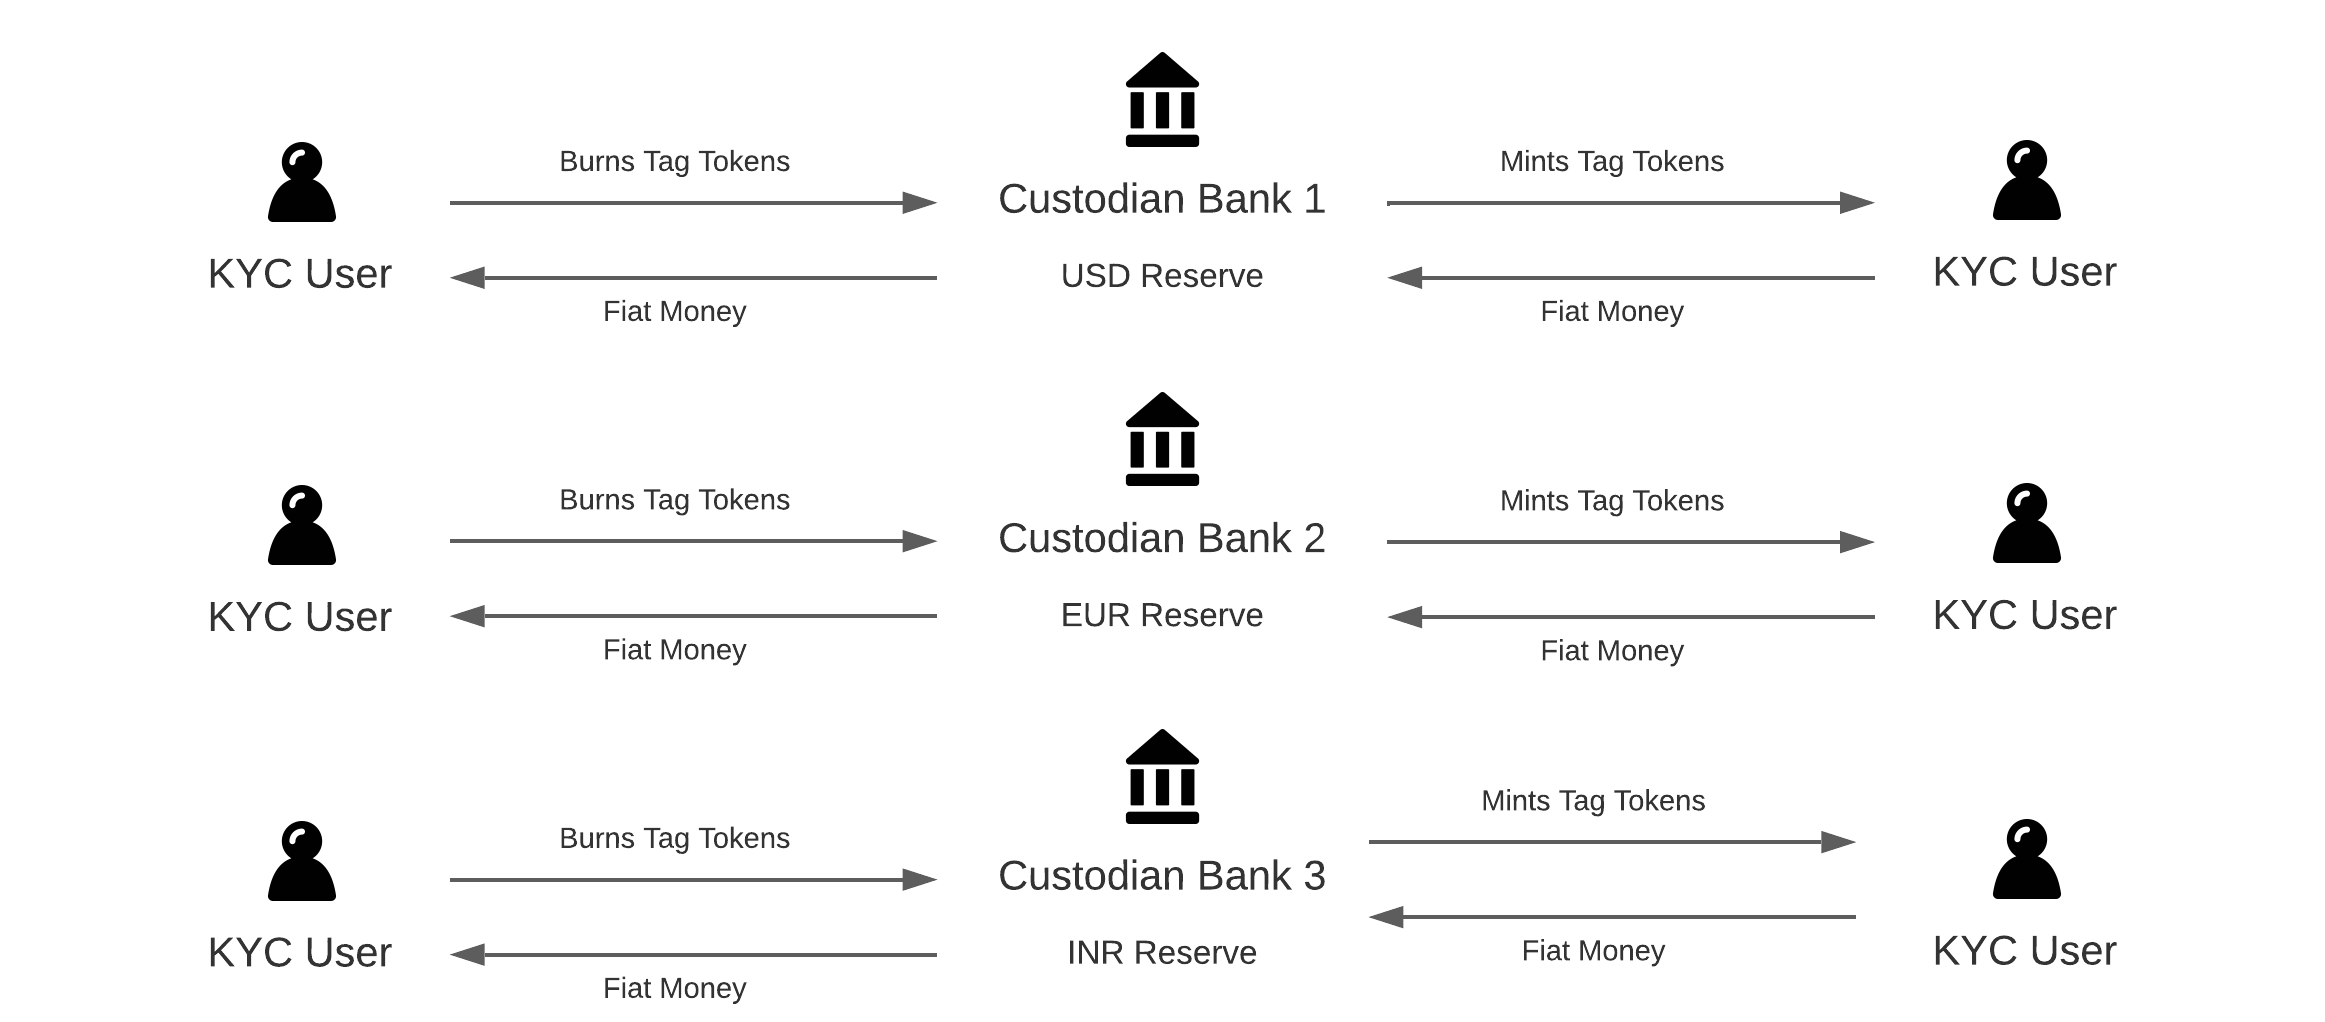
\includegraphics[width=12cm]{custodian}
\caption{Fiat Funds Custodian Banks}
\end{center}
\end{figure*}

\textit{Example}\\\\
Deposit = \$150 ; Method:Bank Transfer\\
$Total\:Mint=150-0 = 150$\\
Total Mint = 150 USD Tokens\\
$Total\:Token\:Distribution=150-(150 \times 0.1\%)=149.85$\\
Total Distribution = 149.85 USD\\
Total Fee = 0.15 USD ; Custodian Allocation = 0.105 USD\\

\textbf{Exchange}\\

Viral-FEX makes use of ViralDEX Swap Book DEXs for exchanging Tag-Tokens to Viral Coin \& Viral Stable Coin. While Centralized order book exchanges holds user's private key, viral-fex supllies tag-tokens that can be exchanged for viral primary coins using a decentralized efficient White-listed liquidity pool specifically for KYC Users.\\




\textbf{Burning Tag-Tokens / Fiat Withdrawal}\\

Fiat-Tag Tokens are burned upon Cash Out request from the KYC User to the corresponding custodian. The Custodian shall burn the tokens excluding the withdrawal fee and maintain the equilibrium of assets on both bank reserve and token circulating supply. The KYC User is required to add bank accounts or payment ids for the stipulated fiat-money i.e., Burning USD requires USD Bank account integration. 

\section{\textbf{Custodian Services}}

Risks of Blockchain\\
Statistics of Loss of Private Keys\\
Problems regarding loss of funds\\
Intro to Viral Custodian Service\\
Overview of the Architecture\\
Advantages of Decentralized Custody\\
Keywords and Security Definitions\\
Vault Smart Contract Overview\\
Creation and Accessing Vaults\\		
Transfers inside Vaults\\
MFA Security\\
Security measures by Trusted Third Parties\\
Possible Attack Vectors\\
Ease of making transactions\\
Competition against traditional banks\\
New Era of simplified custody of crypto assets\\

\section{\textbf{Viral Payment Gateway - Web2 Integrations}}

Importance of Business Transactions\\
Support to Businesses\\
Ease of Transactions, Benefits for E-commerce and Offline Commerce\\
Viral Payment Gateway Integrations\\
SDK - React Native, Flutter, Android Studio, XCode, JS-Web, Xamarin, Ionic, other New Tools \\
Game Engines - Unity, Unreal, CryEngine, GoDot\\
\\
Web-Plugins for No Code Tools - Wordpress, Woocommerce, Prestashop, Magento, Prestashop, Wix, CS Shop, Bubble, Webflow, Shopify\\
Server Integrations - php, python, js, ruby, .net, nodejs, java, go, Kotlin, C\#, ColdFusion\\
Partnership with PSPs (Payment Service Providers)\\

\section{\textbf{ROV - Content Moderation Platform}}

Social Media platforms censor user-generated content to prevent abuse on posts and comments which doesn't follows community guidelines that categorizes illegal, inappropriate, violent and offensive content.  Today's social media has become an integral part of our lives from exchanging valuable information to proving individual ideologies. A vast amount of people receive news from several social media platforms including lawmakers, victimizing people to fake news and conspiracy theories became a common tool for social media users who commit fraud by disclosing fake information to the society. Multiple instances of issuing fake propaganda and government manipulating people by hiding free-speech in democratic countries and the never ending ideological hatred among leftist and rightist have proved a need for a moderation of content spreading across social platforms to minimize violence breakouts. A larger portion of teenagers who use social media are exposed to misinformation and conspiracy theories which are very easily believed.\\

Moderating users content is broadly classified into manual and automated way of moderation. Manual content moderation usually been carried out by humans by hiring, training them to analyze, review and make decisions based on the provided community guidelines of the platform. Large platforms employ moderators based on contracts whereas small platforms employ moderators full time. Automated moderation involves finding flagged contents across the platform and deciding to remove the contents of the  particular post. AI methods lacks accuracy in several free-speech category hence used only in particular areas like Nudity, sexual abuse, etc. Automated moderation decides to remove flagged contents using predefined set of databases and trained models based on regional laws and datasets that collected over years.\\

Methods of moderation falls onto three categories which is used in nearly all the platforms as a counter-measure to increasing terror and illicit activities across the globe in which social media plays a huge role by sharing information to the global communities. The categories are
\begin{enumerate}[wide, labelwidth=!, labelindent=0pt]
\item \textbf{Pre-Moderation} : An automated way of moderation which involves screening the content of the post (video, photo, text) before it is published. Pre-moderation is commonly used for finding copyright materials, nudity, child abuse which can be explicitly found out with high accuracy by the deployed automation tools
\item \textbf{Post-Moderation} : A specific type of moderation which searches for in-appropriate content across the platform proactively after the content is displayed to the users. Conversions and publications takes place in real-time with post-moderation which aids to a fast paced platform. This method is criticized due to the legal rights given to the platform owner for publishing and taking down the content.
\item \textbf{Reactive-Moderation} : Depends on active contribution by users to flag or report contents which they feel inappropriate and considered as not safety for the global community. This usually carried by placing a report option in every post on the social platform. Moderation scales with addition of users to the platform which helps in better \& faster moderation of contents.
\end{enumerate}

Companies like Facebook, Twitter and YouTube uses a combination of tools with a hybrid mechanism of multiple moderation methods such as pre, post, and reactive moderation to search out and remove posts \& user comments that violates their policies with the help of automated AI Tools and unbiased human moderators for higher accuracy. While moderation emphasizes safety and prevents spread of fake information, popular social media platform owners/entities misuses the authority of moderating user's content in several sectors. Private account contents are being displayed to moderators which facilitates breach of privacy, and sideways working with regional governments to moderate free-speech anti-governmental campaigns to safeguard their existence in a particular region proves a biased employee platform that misuses the governance over people's original content. Entities governing the platform deletes or expel users without a notice which eliminates the trust in these platforms. Usually, content moderators on existing social platforms will be held responsible for removing illicit content whereas sometimes due to a centralized approach these moderators are told to filter independent content posted by creators on certain topics for governmental advantages.\\

Moderators who are employed by popular social platforms through third party company contracts are also facing issues by these parent entities controlling the rules of their daily-work by forcing them to review photos and videos consistently for 12 hours combined with strict schedules and aggressive quotas leaving them traumatized. While Automated filtering algorithms aren't accurate for filtering user based content, manual moderation is the key for a free-social platform which also has cons among the moderation community to watch inappropriate violent content such as child abuse, suicide, terrorism, etc. Moderators constantly sue platforms over enforcing maximum work-load a day for moderating traumatizing content without providing emotional support for mental breakdowns.\\

To counter these issues faced by users and moderators, a decentralized moderation community solution is proposed in the white-paper for the viral social network to ensure independent content creation without the external influence of any third parties such as governments, large entities and also to provide removal of explicit content in a faster and a well managed democratic way using a new vote-based consensus moderation. Moderators are well compensated for their contribution and will have all their fundamental-rights for reviewing illicit content without external pressures given similar to centralized companies. The administrative rights of removing content is provided to swarm of moderators deciding to remove inappropriate content based on majority voters decision. Meddling of centralized companies are eliminated making Viral a truly decentralized social platform with content moderation benefits for a cleaner content-based platform.\\

\textbf{ROV - Republic of Viral}\\

ROV is an abbreviation for Republic of Viral, a decentralized community-based organization inside Viral Network to govern, filter out reported contents, give support to users, verify VIPs, vote on involvements of community members, etc. The Community is solely developed to bring a decentralized way of allowing a network of administrators (moderators) under a voting mechanism to remove NSFW, spam content in the Viral Network under it's updated community guidelines, and aims to create a cleaner social media while restraining the power of censorship resistance. ROV is designed for curators (moderators) to work as employees of an organization with a common goal with maximum trust and anonymity. This decentralized way effectively reduces the opinion of a single person, an entity’s founder, and any external influence where the community only decides which is better for the platform to display. ROV eliminates the need for a centralized entity to run a social platform that holds the power of democracy while ignoring censorship resistance. \\

Viral employs both automated AI tools and human based moderators for reviewing in-appropriate posts circulating the viral social platform. Viral makes use of three different models on moderating content, that is
\begin{enumerate}[wide, labelwidth=!, labelindent=0pt]
\item \textbf{Reactive Moderation} : Posts manually reported by viral users, reviewed and taken down manually by ROV curators.
\item \textbf{Pre-Moderation} : Automated algorithm runs before publishing to prevent posting contents that emphasize nudity, bullying and abuse.
\item \textbf{Hybrid Post-Moderation} : Involves automated tools to find illicit content of public accounts, reviewed and taken down manually by ROV curators.
\end{enumerate}

\textbf{Reactive Moderation of Content}\\

Reactive Moderation is a manual yet highly scalable method that involves both normal users and rov-curators collectively work to filter out contents that doesn't fit the community guidelines \textit{(which will be available to all the curators and users after the alpha-release of the viral social platform)}. User reports an in-appropriate content under a certain category is published as a poll in the ROV application under a certain time limit in accordance to the category, reviewed and voted by the curators which will be decided on majority's vote to keep or take it down.\\

\textbf{Moderation and Manual Removals}\\

To remove a post in centralized social media, the entity governing the application shall remove the user's database tables that contains the post-meta data. Post Metadata is defined as the data providing information about one or more information about a post i.e., image url, description, etc. Unlike centralized social media, Viral is a decentralized social media that doesn't owns user's data, hence Viral and it's developers doesn't have governance over users meta-data. For a clean, appropriate content platform moderation is a key for it's growth. Viral proposes to solve moderation issues by removing the media's source from it's Viral Private IPFS Clusters by publishing the black-listed media live using decentralized oracle's.\\

Viral's IPFS cluster which is explained in the User Security and Privacy page of the whitepater, replicates data across trusted high efficiency IPFS nodes for a decentralized censorship resistant storage. Viral IPFS Clusters have the authority to remove data/files from it's nodes by fetching black-listed files fingerprints from ledger maintained through decentralized oracles - resistant to data tampering.\\

\begin{figure}[H]
\begin{center}
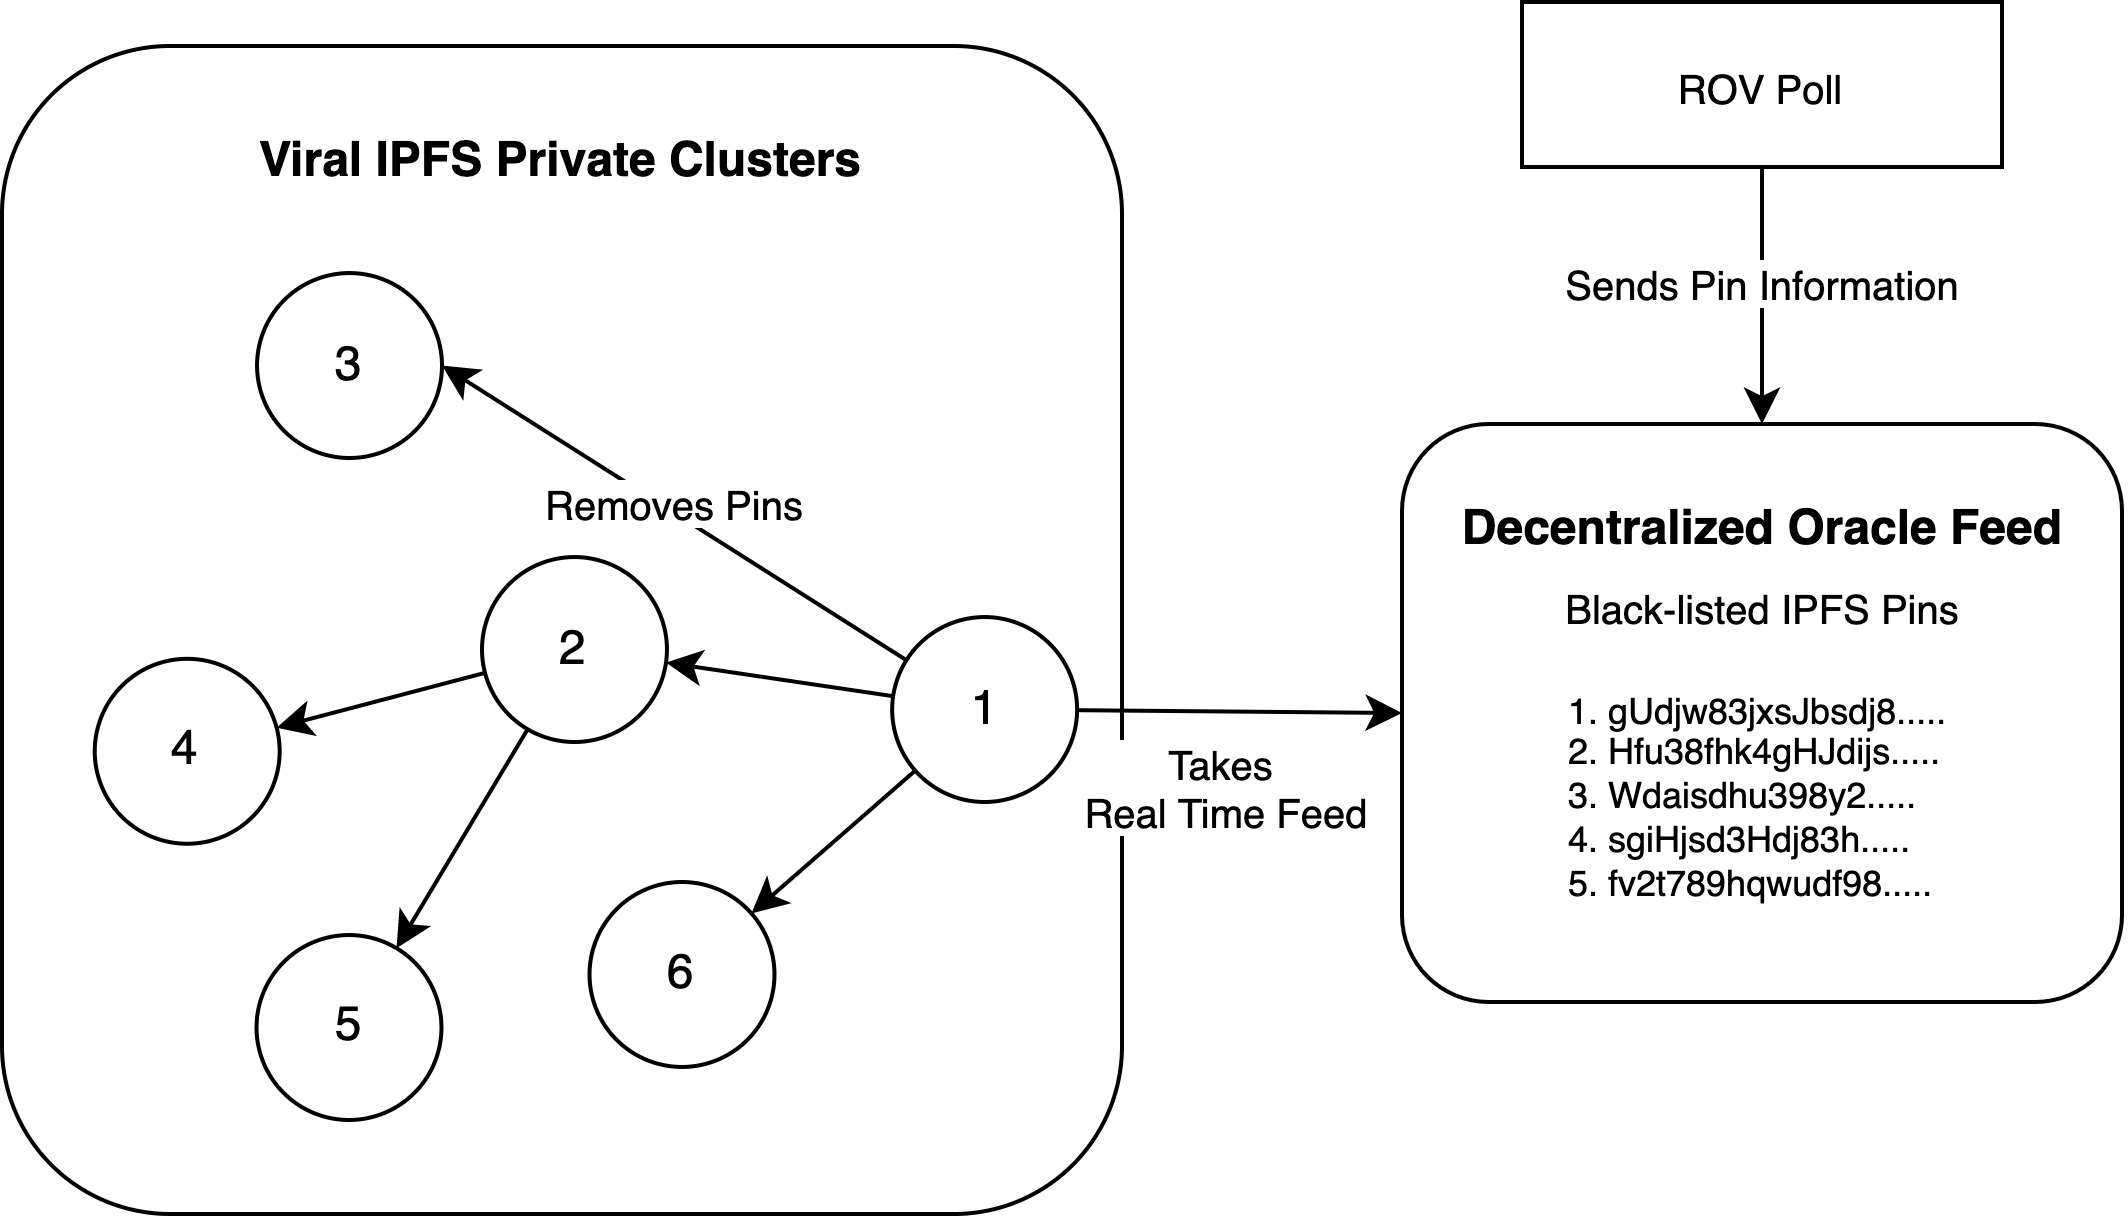
\includegraphics[width=8cm]{content-removal}
\end{center}
\caption{Blacklisted Pins Live Oracle Feed to remove content across Viral IPFS Cluster}
\end{figure}

\begin{itemize}[wide, labelwidth=!, labelindent=0pt]
\item ROV poll is conducted among the curators of the platform to decide on to keep or remove the post.  After deciding on removing the post,  the IPFS CID \textit{(content identification)} of the post is sent to a decentralized oracle ledger for immutability and tamper-resistance
\item The Oracle feed displays blacklisted CIDs for the Viral IPFS Cluster Peers/Nodes to publish a remove command to the cluster layer
\item After the pin remove command is published the peers within the cluster removes the pin from their respective nodes
\item A garbage collection is run on the peers and the content is removed completely from the viral clusters
\end{itemize}



\textbf{Removal Poll Timer}\\

To ensure faster removals and counter the delay of manual approach of votes calculation, after content is reported it will be directly posted on ROV’s Application where the voting poll for the specific post timer will run according to the category’s emergency for removal. This ensures faster content removals in no time, where it takes 24 – 48 hours for a centralized social media entity. We have listed out the major categories and timings for reporting illicit content in Viral.

\begin{itemize}[wide, labelwidth=!, labelindent=0pt]
\item Spam or Fraud – 2 hours
\item Bullying or Hate Speech – 45 mins
\item False Information – 1 hour
\item Sexual Harassment - 30 mins
\item Nudity – 30 mins
\item Violent or Disturbing – 30 mins
\item Something Else – 2 hours
\end{itemize}

\textbf{Algorithmic Automated Removal Methods}\\

Additionally, to improve faster removals an algorithm is proposed to finish the poll timer if the votes are more than 10 and 90\% have voted to remove content or keep content. This effectively eliminates the possibility of waiting to remove the content till the timer ends, if the post is in a high state of emergency to remove. By taking,
\begin{center}
$\lambda$ = Total Votes, $\gamma$ = Total Remove Votes, $\kappa$ = Total Keep Votes \\
$\gamma_p$=Remove Votes Percentage, $\kappa_p$ = Keep Votes Percentage\\
\end{center}
\[\lambda \geq10\]
\[(\frac{\gamma}{\lambda}) \times  100 = \gamma_p \geq 90\]
\[(\frac{\kappa}{\lambda}) \times  100 = \kappa_p \geq 90\]

\textbf{Process of Polls}\\
\begin{figure}[H]
\begin{center}
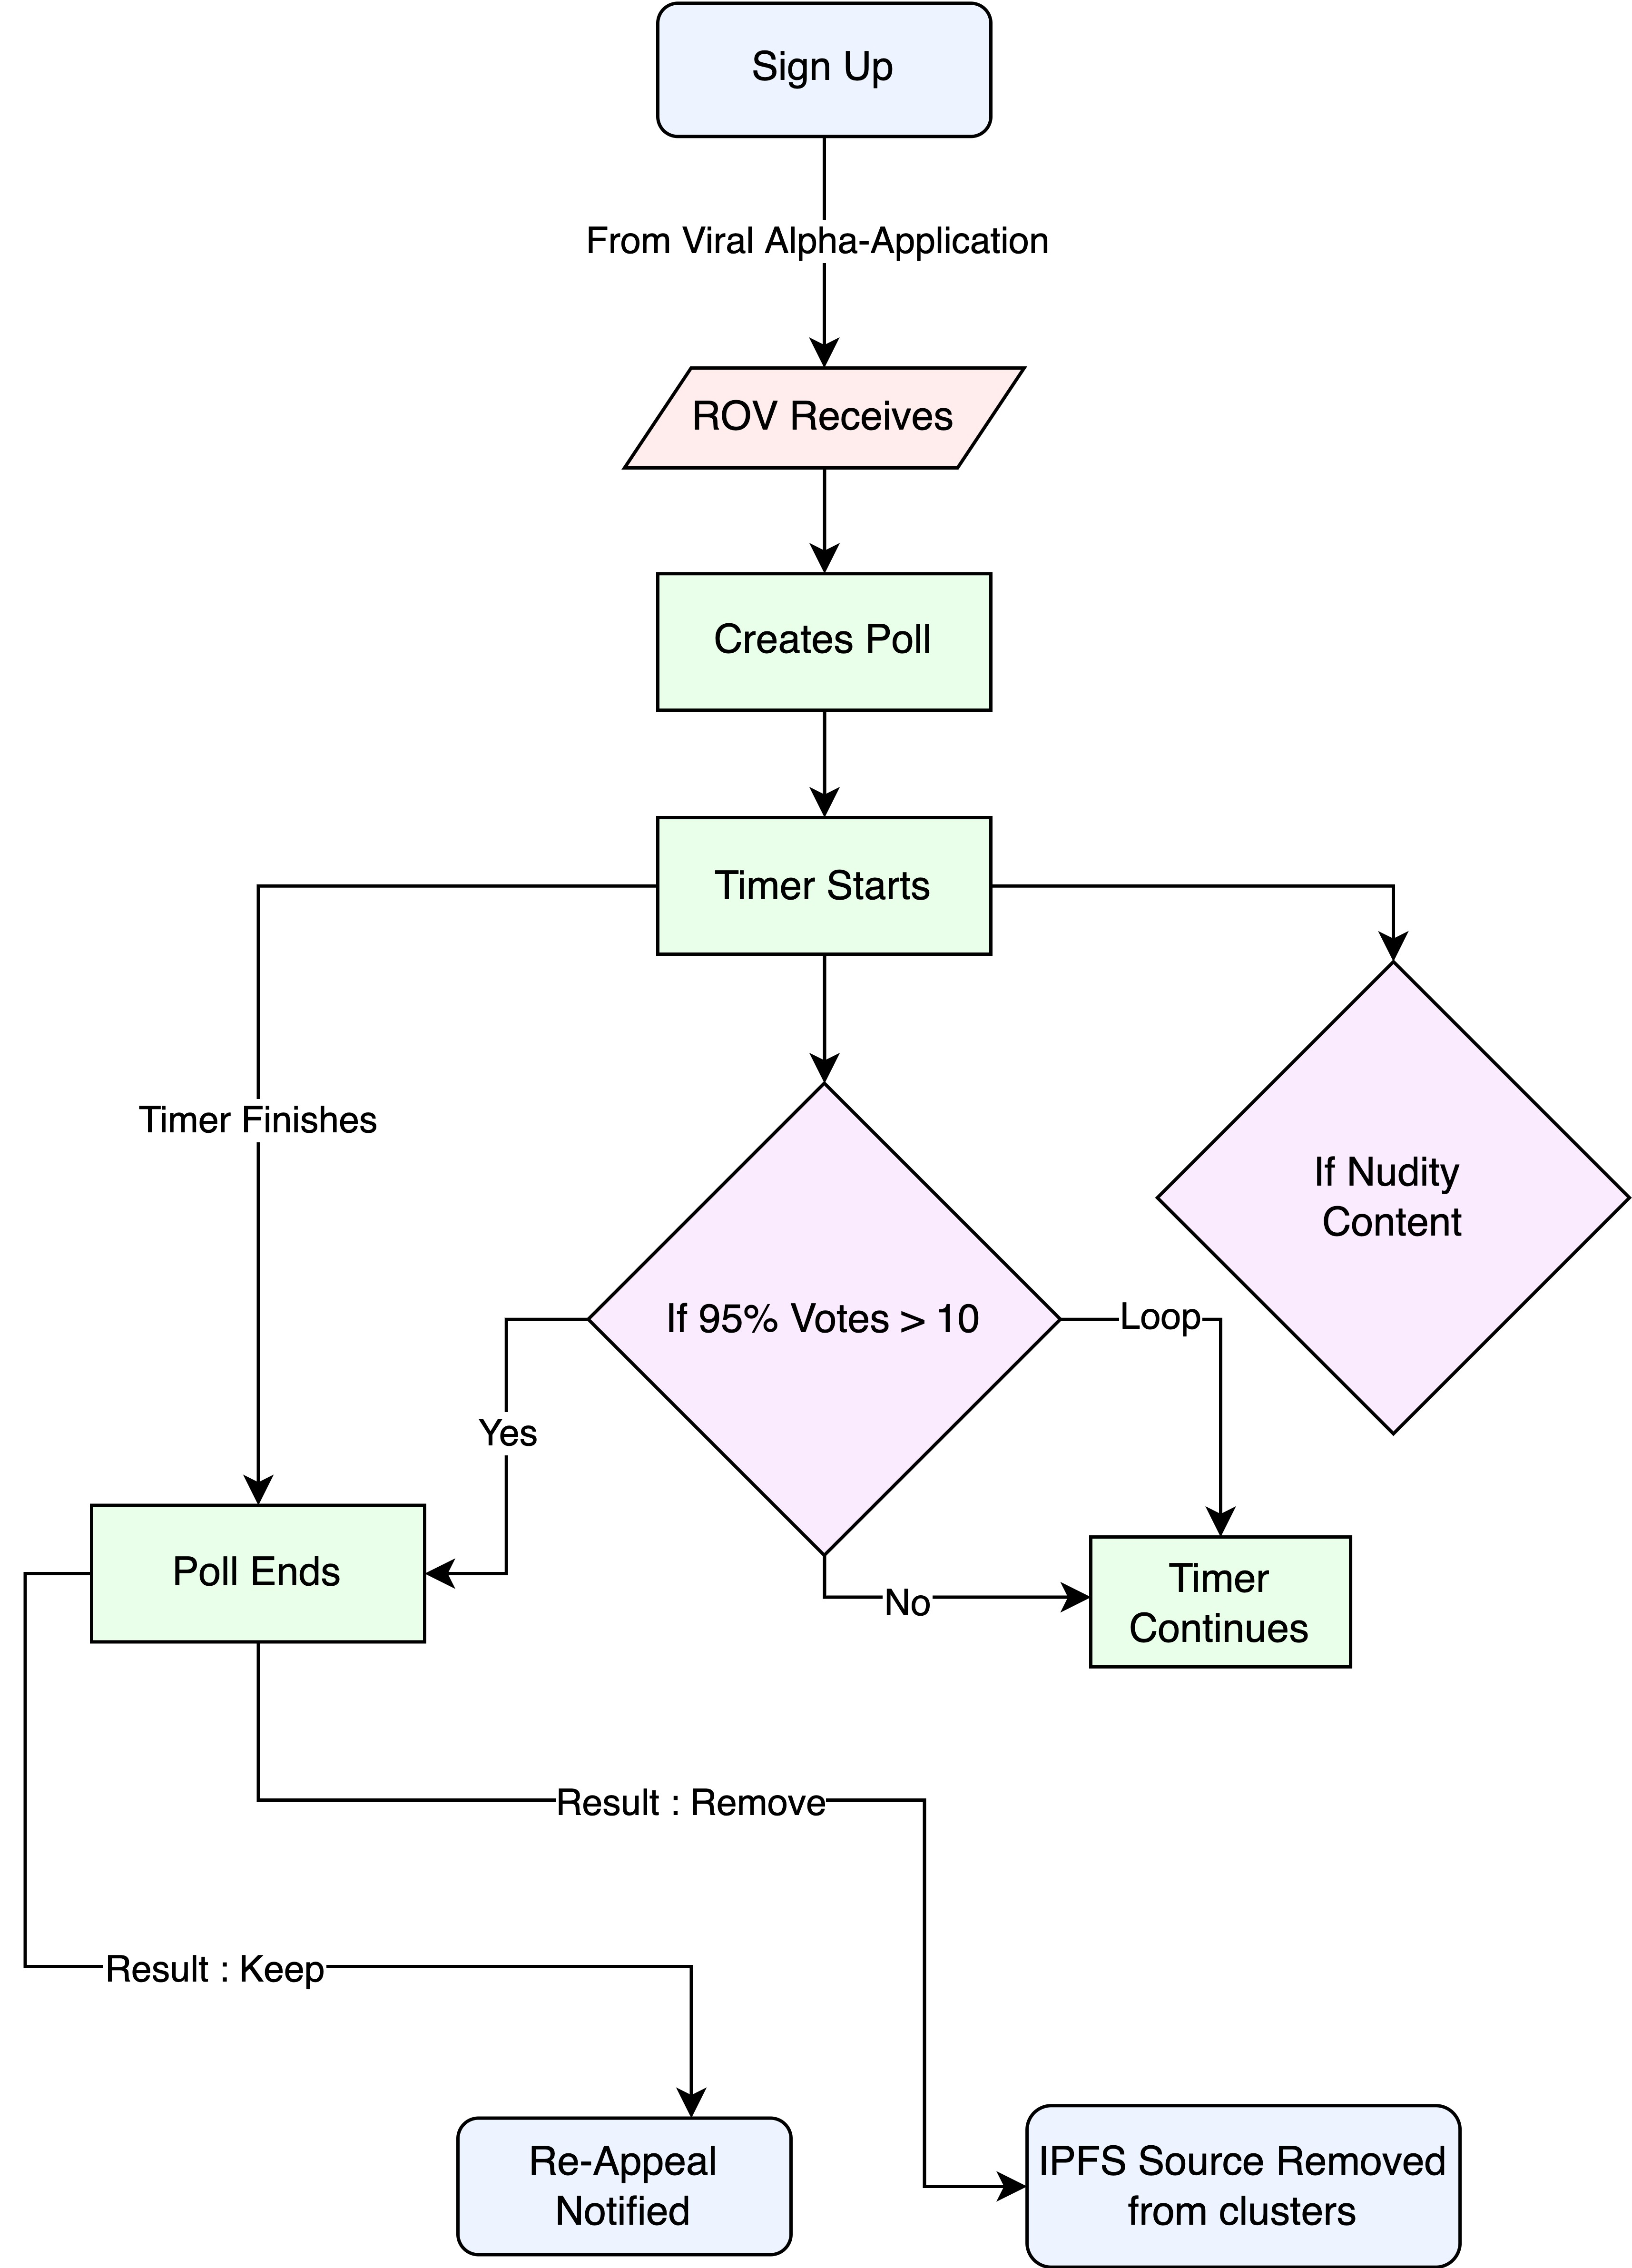
\includegraphics[width=7cm]{rov-poll}
\caption{Glimpse of ROV Process}
\end{center}
\end{figure}

The reactive-moderation type polls are initiated  in the following steps,
\begin{itemize}[wide, labelwidth=!, labelindent=0pt]
\item A user reports a content in the viral social platform which he/she feels in-appropriate for the community or similar viewers
\item ROV receives the report under reactive-moderation and creates a poll for the reported user to review, analyze the content for further action
\item A timer is added in the poll according to the category of report chosen by the reporting-user.  This allocates certain very important categories to be shown first to the active curators.
\item The poll receives votes based on the curators opinion and the community guidelines followed by the curators. Both "keep" and "remove" votes are calculated until the timer ends
\item A premature poll ending algorithm runs with every single vote to determine the chances of ending it.  The poll ends if the algorithm satisfies the condition of 90\% of more than 10 votes are voted towards a single decision.
\item After the Poll ends the decision is taken by calculating the majority of votes. 
\item The content is removed from Viral IPFS Clusters or kept for further appeal if the curators decision was to keep the content.
\end{itemize}


\textbf{Re-Appeals}\\

Re-appeals are similar to regional court's first \& second appeals done by individuals against the decree of the jurisdiction.  Re-Appeals are given to the users of Viral to re-report against the decision of curators while giving an explanation for removing the post where the ROV curators can again vote and decide to keep or remove based the content by taking the explanation given by the user who re-reported. Re-appeals applications will expire in 48hrs after the first-decision is posted by the ROV curators to keep the content. \\

The algorithmic premature poll ending timer for re-appeal is posted two times ($2x$) the category timer for normal reports where if votes are more than 25 and 70\% opt again to keep or remove the content the timer will end prematurely.\\
\[\lambda \geq25\]
\[(\frac{\gamma}{\lambda}) \times  100 = \gamma_p \geq 70\]
\[(\frac{\kappa}{\lambda}) \times  100 = \kappa_p \geq 70\]


\textbf{Pre-Moderation \& Post-Moderation using AI Tools}\\

Pre-moderation also known as screening is carried out locally on the device to restrict publishing adult content on the social platform. Various nudity detection programs are available as open source which can be leveraged to develop a minimal version which can be run locally within the device. Post-Moderation requires multiple machine learning \& artificial intelligence tools which can be actively developed by the Dev-Space Community \textit{(further explained in Developer Platform section)} which can find for flagged contents and report it to the ROV-community. Nudity and pornographic contents will be removed at instance if the accuracy is higher using automated tools.\\

\textbf{Private Accounts}\\

Viral’s content reports are only applicable to public accounts. Viral’s vision to bring complete privacy and security to private accounts which are exempted from being reported.  Every single content in the viral platform is encrypted, the curators can only view the public content as a watcher \textit{(explained in the User Security \& Privacy section)} due to it's publicly available decryption keys. ROV curators will not moderate, nor involve to view the contents of secured private accounts. Thus, it leaves decisions in the hands of followers whether to view their content or not. \\

\textbf{Eliminating Bad Curators}\\

To eliminate biased curators we will be bringing a safe mechanism to filter out bad curators in the community using a feature called positive/negative points. Every single poll will contain two options for the curators to select, “Remove” or “Keep”, the poll results are based on the majority’s decision. When a vote for a poll and falls under the majority’s vote the curator will receive a Positive point, if the curator is on the minority side, which is the losing side he/she be getting a Negative point. Each of the positive and negative points will be added to his profile. An algorithm will run to take the percentage of both points, where if the negative point falls above 30\% to the positive point, his ROV account will be suspended for a couple of days. We have deciphered the factors where there could be no bad actors in the community. There will be records to everyday's positive and negative points. This Positive/Negative points suspension factor will be running after every single vote after the poll finishes. Some factors determining the suspension are\\

\begin{itemize}[wide, labelwidth=!, labelindent=0pt]
\item If Negative Point is 30\%- 40\% to the Positive Point – Account suspension for 3 days
\item If Negative Point is 40\%- 50\% - Account suspension for 6 days
\item If Negative Point is more than 50\% - Account suspension for 12 days
\end{itemize} 

Taking Negative Point as $\eta$ and Positive Point as $\rho$

\[(\rho) \times  30\% \leq (\eta) \leq (\rho) \times  40\%\]
\[(\rho) \times  40\% \leq (\eta) \leq (\rho) \times  50\%\]
\[(\rho) \times 50\% \leq (\eta)\]

We have also made factors to suspend an ROV account forever based on the number of suspensions they get on their account. The factors are
\begin{enumerate}[wide, labelwidth=!, labelindent=0pt]
\item 20 times 3 day suspension 
\item 10 times 6 day suspension
\item 3 times 12 day suspension
\end{enumerate}

There will be a test-net and live-net to practice voting at its best\\

Example : \\

User A: Day 26; Positive – 234; Negative – 80; Result: More than 30\%: Suspension for 3 days\\
User B – Day 30; Positive – 523; Negative – 343; Result : More than 50\% : Suspension for 12 days\\


\textbf{Community Help \& Support}\\

ROV will be having a separate section for community help \& support, where ROV curators can easily offer their support to Viral users by providing them answers for their queries through the application. The Curators will act as support persons for their issues and thereby providing answers for their problems. It will be a decentralized substitute for centralized customer support. Since the curators cannot offer custom support by an admin staff in a centralized company rather, they can offer support for their questions regarding the usage of the application. For every contribution by the curators, they’ll receive their fair share of rewards.\\

\textbf{Verification of Accounts of Celebrities}\\

ROV curators also will be responsible for several actions on the decentralized platform, one of it's the "Verification of Accounts". Since Viral doesn’t take a single byte of data, viral won’t be requesting any country’s identification information like other centralized social medias, it is up to the curators to opt for giving a verified tick for the VIPs on the viral platform. Curators vote on Providing Verification where the majority votes decide the verification of a specific individual or organization. Users applying for verification can provide additional data such as popular media websites blogs about them, provide a verification video and also tip the rov community on whole to provide verified tick.Verified Tick is represented by a unique NFT minted by the user after ROV's approval.\\

\textbf{Requesting ROV}\\

Since ROV is regarded as a DAO (Decentralized Autonomous Organization) we make sure others request ROV for a specific task, poll, support, etc. This feature will be given only to verified profiles where they can write to ROV in any matter where the curators can come collectively to help regarding the issue. This will help VIPs, Governments to write to ROV curators which will be displayed on their feed where they can take necessary actions for it. \\

\textbf{Curator App Overview}\\

ROV will be having a separate Mobile Application for curators and moderators to easily vote for reported contents using swipe methods similar to dating apps. Since ROV is a restricted content application it will not be available on the mobile applications stores. The Application will be only available on Android as a 3rd Party App and won’t be available for iOS devices due to their security policies. This application will be providing productive features for curators to vote on moderating reported content. \\


\textbf{Rewards for Contribution}\\

Every day according to every individual curators contribution rewards will be allocated to their wallets where they can collect it manually after 2AM UTC.  More information on reward allocation for ROV curators is explained in the Global Reward Pool section.\\

\section{\textbf{Developer Platform}}

Open-Source projects are considered as free revolutionary software-technologies in competition with profit-making closed source projects developed by monopoly companies under a team of few high-equipped developers. During the time of internet and usage of computer softwares, a look into source-code with a collaborative structure of development of a particular software built trust among developers and aided to better performance and flexibility. The “open source” label was created at a strategy session held on February 3rd, 1998 in Palo Alto, California, shortly after the announcement of the release of the Netscape source code. By realeasing their code to the public Netscape has illustrated a valuable way to engage with potential software users and developers, and convince them to create and improve source code by participating in an engaged community. The emergence of popular projects like Linux, a Free Open-Source Operating System, released under GNU General Public License (GPL) became the largest open source project in the world shortly after Linus Torvald and 100 other developers launched version 1.0 of the Linux Kernel  on 1994 as a free, alternative Operating System to other UNIX based closed sources at that time.\\

Although most people are rooting for free-softwares the open source projects are mostly lead by groups of developer communities and are discussed and built among white-listed communities due to lack of tooling available for collaboration. By 1999 Source Forge was developed as a collaboration tool where developers can host, manage their code for free and resolve bugs together in one place. These collaborative tools are known as distributed version control systems. While most tools improved the open source initiative, it was Git which revolutionized the distributed version control system by storing references to file snapshots instead of storing list of file changes like other tools in the market. By 2008, Open-source projects became more popular among developers to collaborate in interesting projects with Developer Q/A platforms such as Stack Overflow later expanded to network of Q/A sites which collectively called as Stack Exchange.\\

The inception of Open-source has paved way for the birth of blockchain technology that we see today as a pioneer in financial and immutable applications sector. Although Open-source and Block-chain technology serves different ideologies and techniques, we can see the qualities of both running parallel to each other. The motivation in open-source platforms drove the emergence of block-chain technologies. Almost all the prominent cryptocurrencies in the market, including Bitcoin and Ethereum, are open source. Their design and codebases are available in the public domain. 99\% of all the projects built on top of blockchains are open-sources are driving the most developer activity. These are some of the hundreds if not thousands of ways that blockchain is being implemented with the help of open source collaboration amongst developers across the world. There’s no doubting that open source is a major driving force behind the rapid development and deployment of blockchains across a variety of industries. The creation of blockchains on such a vast scale would have been impossible without open source management systems like GitHub and BitBucket, as well as a version control system like Git. The blockchain revolution is being powered by open source.\\

\textbf{Building a Paid Developer Platform}\\

Developers work with Open-source code improving and building upon it to create better version of the current software. The source code is made available online under specific license to modify, edit or distribute the software. Most of the open source project's initial versions will be built by the founding organization's bootstrapped developers and later the bugs and issues will be resolved by open-source developers by contributing their time, skill and effort. Software users leave feedback and problems they encounter along with new feature requests to make the software more user-friendly and functional.\\ 

Some of the well-known benefits of building an open-source software are
\begin{enumerate}[wide, labelwidth=!, labelindent=0pt]
\item \textbf{Lesser Costs} : Open-source software eliminates the fees involved in commercial softwares on licensing and maintenance, while reduces expenditures on documentation, media and support
\item \textbf{High-Quality Software} : The availability of source code is well audited by various developers producing a neater and a well-structured code base efficiently used for building on top of it.
\item \textbf{Huge Support} : Easy access to internal code of the available software increases the chance of greater support from online communities, centralized organizations, freelance spaces to grow a well-developed software
\item \textbf{Speed of Development} : Open-source enables the world of instant issues solving community that can offer faster results in terms of bug fixing, feature building, etc
\item \textbf{Improved Security} : Building a safer software by issuing transparency for every white-hat professionals in the world to review, find vulnerabilities to constantly build a safer, stronger software
\item \textbf{Innovation Exchange}: New disruptive features will be contributed by individuals and entities sharing their innovation driving a creative work-space for other developers working on the open-source project.
\end{enumerate}

Usually open source developers earn from their regular jobs and does not get paid for their contribution to the source code of the project they are working on. Companies that bootstrap the development of open source projects builds it using developers they hire and release it open-source for anyone to fork and make necessary changes to the code. Companies doesn't track contributions and it is upto the developer to choose what he/she finds interesting to work on with or without getting paid. Organizations like RedHat, IBM, Oracle employs developers and pay them accordingly for working on several open projects. Open Source initiatives brings better flexibility of acquiring free developers around the world but majority of the organizations doesn't provide any incentives or a financial motive for a quality source code.\\

The Viral Network of applications provide a new initiate known as "Paid - Open Source Initiative (POSI)" through a open platform/space which allocates incentives for every developer contributing to the repositories source codes without a central entity's authority making it a fully decentralized system leaving the reward allocation of every single developer into the hands of fellow community developers eliminating an elected leader. The platform is named as "Viral Dev-Space" and it comprises the solution provided to develop viral open-source projects seamlessly with forward and backward communication between developers and incentive them accordingly for their contribution every day from the global reward pool.\\

\textbf{Viral Dev-Space}\\

Viral Dev-Space, a platform for developers to develop, communicate together with other experts, and receive rewards for their contribution to the Viral Open-Source applications and future development plans of the public and the Viral DAO. The Space for developers is created to decentralize and automatize the Software Research \& Development sector of Viral Applications in an efficient way by providing rewards in Viral Coins through unbiased voting based on the intensity of their contribution and popularity in the development community.\\

An opportunity for all developers is provided regardless of their educational background, region, and language to work on improving the viral decentralized applications on fields such as security, interoperability with other social giants and also to make the application bug-free while providing new updates to the beta software which will be available as an Open-source repository. Giving new opportunities to develop for an upcoming massive social network will pave a way for fastening the development process by the potential of mass development techniques.\\


\textbf{Platform Overview}\\

A web application is provided where developers can join, interact in development groups and receive rewards daily every 24 hours according to their contribution. This application will be maintained by Viral DAO. The App will serve as a community platform where any developer can choose their favorite preferences, communities, and development projects. Developers can choose the project of their preference by searching and also by opting for an interactive questionnaire to find out which project is suitable for them. After giving their preference they can choose the project they want to work in. The developer will have a limit of working on two projects at a time, where they can remove themselves from the project team and opt for other projects as well. This will ensure that developers will have an increased productivity and a higher success rate in specific projects.\\

\textbf{Viral-Github Integration}\\

\begin{center}

\includegraphics[width=4cm]{git-int}
\end{center}

Developers are registered by integrating their git-hub profile with their viral username on the dev-space application. Since viral immutable user name is the native smart chain's name service system that transports the assets to the public address linked up with the username. This allows developers to sign-up with the viral social application by registering their usernames and creating viral smart wallet, etc for receiving incentives on their daily contribution. Github profiles with commits and merge requests to viral projects main/beta repositories is monitored and feeded to the dev-space specific project's feed for other developers to give shout-outs to their favourite commits to give them increased amount of incentives.\\

Viral makes use of git version control system to keep track of changes made by whom and when those change were made to the code repository. Viral Foundation, the only central entity will be provided the administrator rights that maintains the hosting of repositories through Github, the most popular code hosting provider commonly used by developers around the world. Viral Dev-Space developers can work on repositories by cloning available projects, creating their own copies, making necessary changes and merging them to the development branch repository after the code is peer-reviewed by the open-source developers employed by the Viral Foundation.\\ 

\textbf{Work-space overview}\\

Dev-Space from Viral is a open communication platform for developers that comprises of chat groups, sub groups, feed, reward determination programs, project initialization, collaborator network, vulnerability section, etc that will help in an automated workspace environment for quality collaboration for seamless distributed development. Every developer profile will be publicly accessible which is integrated with their individual viral profiles. List of projects, detailed description, successful merges, codes under review, chat pages \& recent interaction between developers will be available for an open audit by any viral user. Each project will have different chat channels (E.g., Back-End) based on development sector of the current project which will also includes sub-channels (E.g., Database Management) for better communication among team of public developers. In short, Dev-Space is a communication \& reward platform for viral Paid Open Source Initiative (POSI) developers.\\

\begin{figure*}
\begin{center}
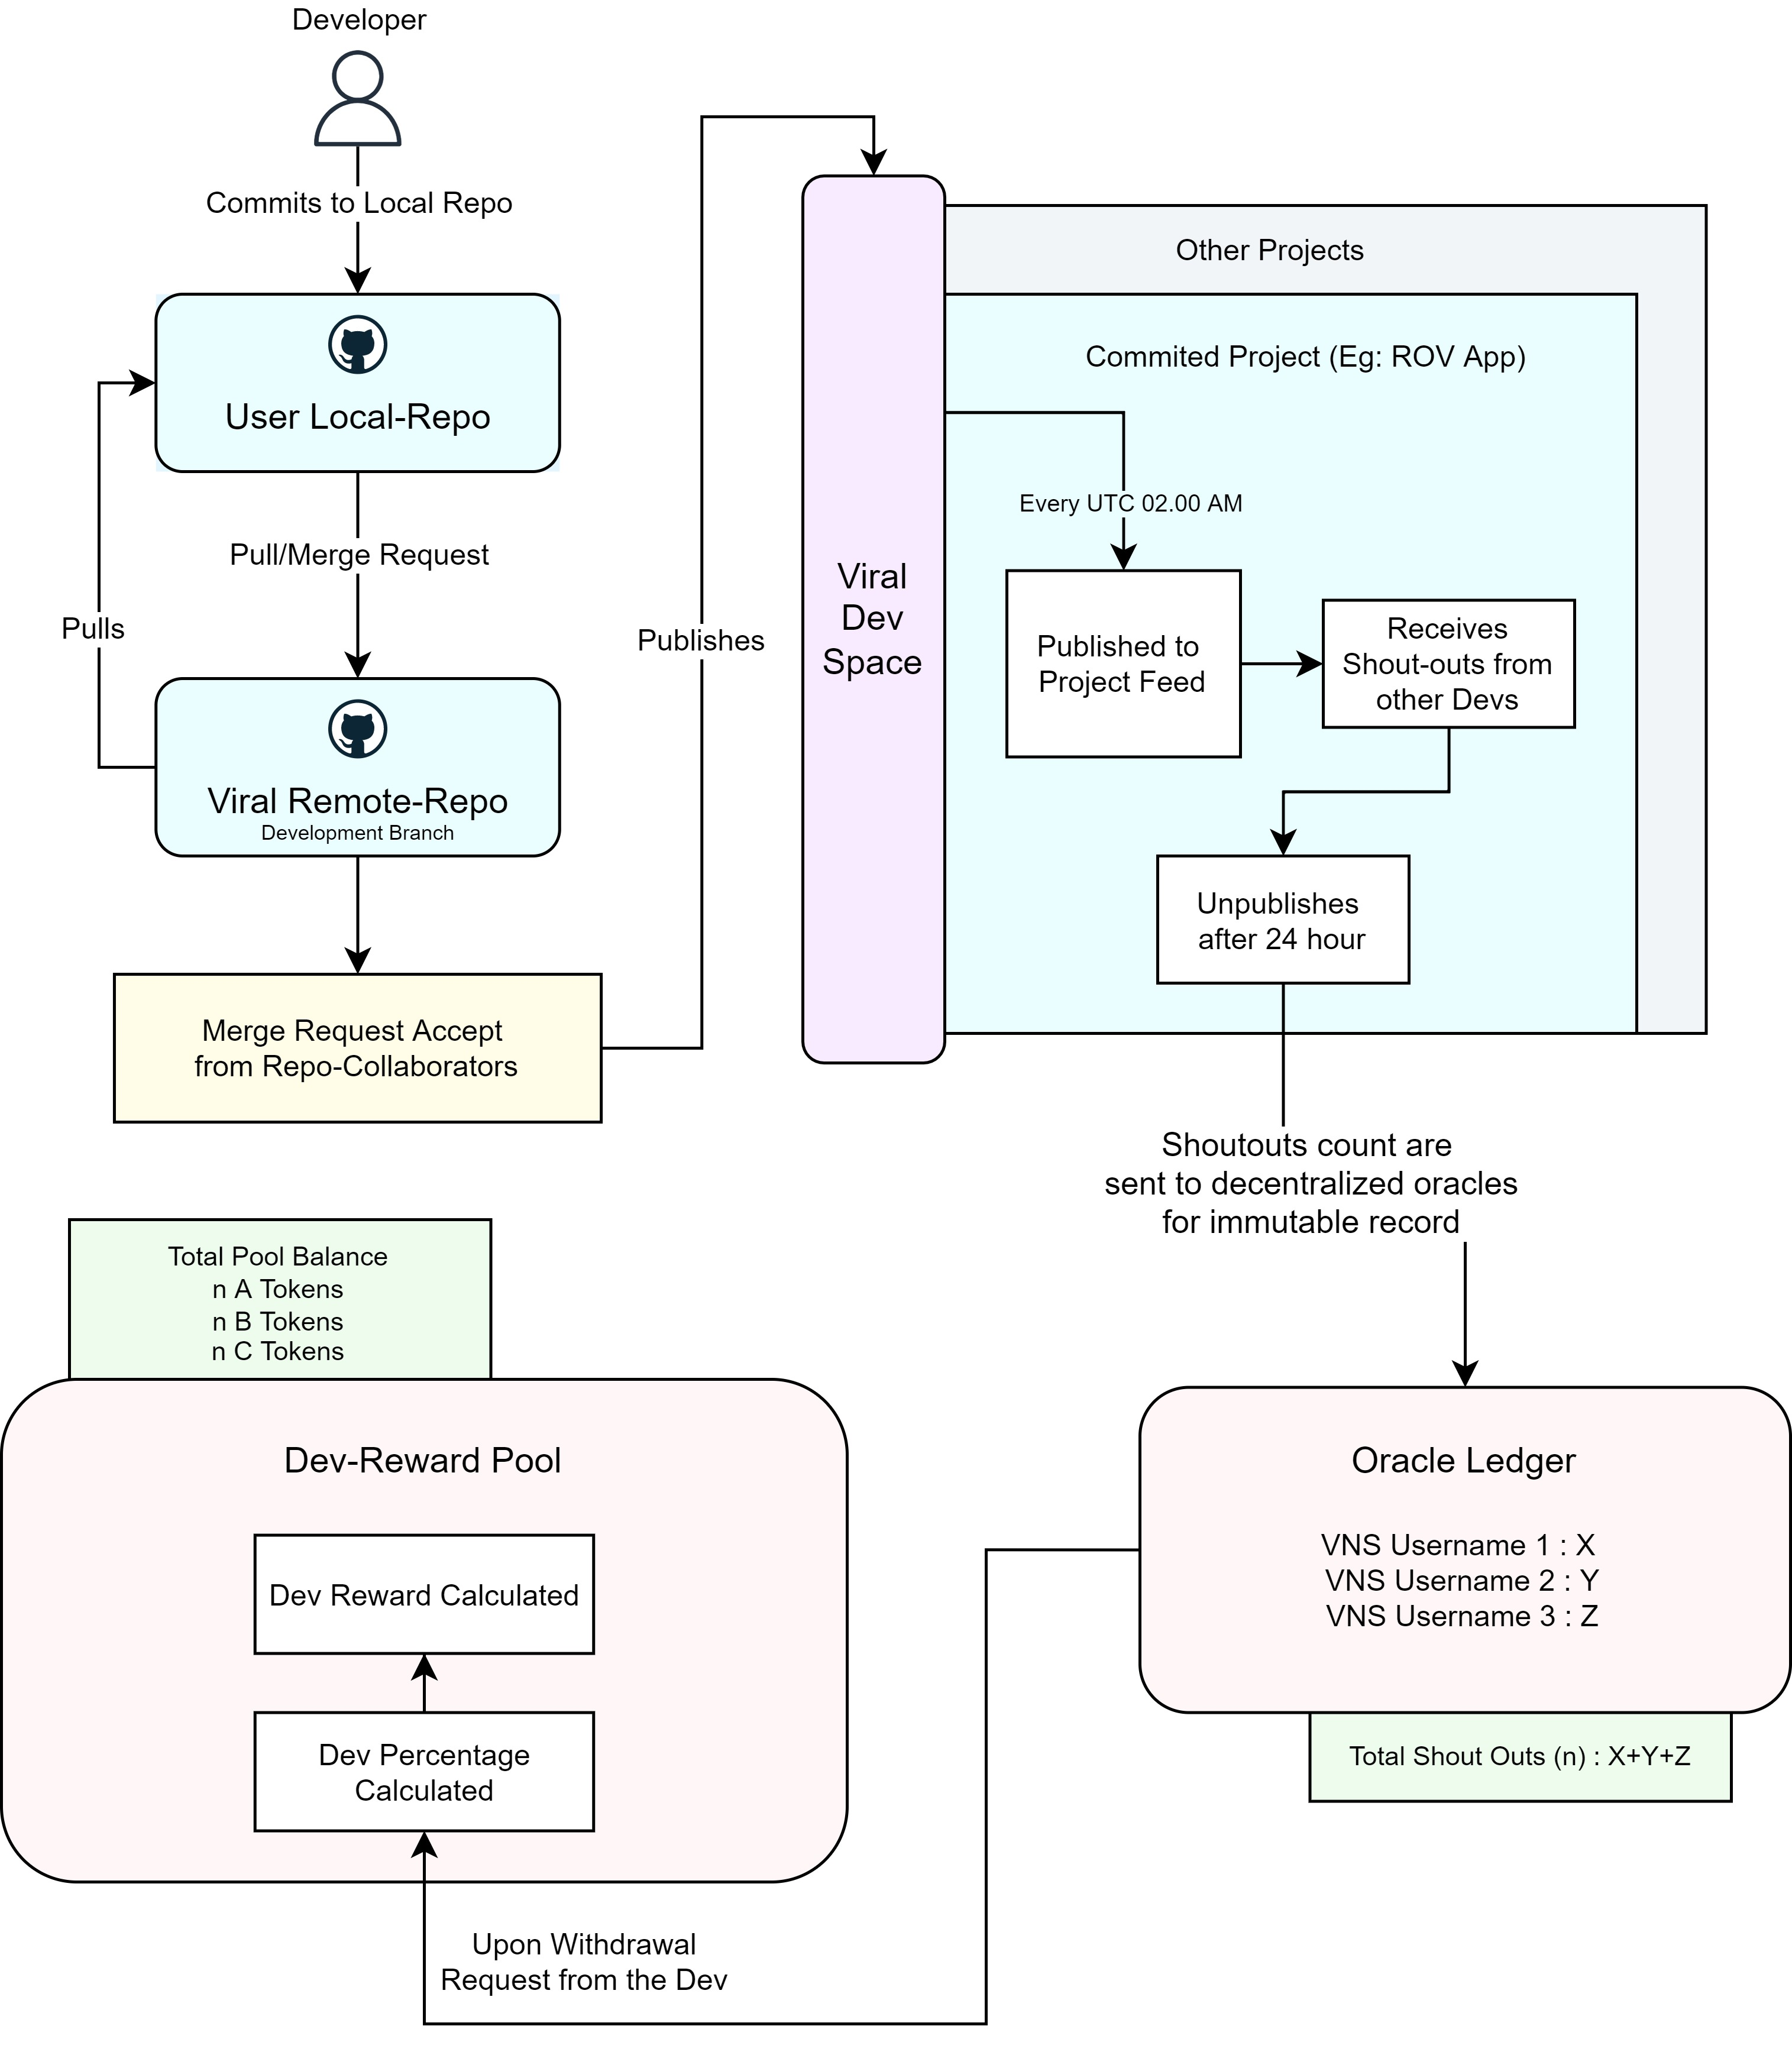
\includegraphics[width=13cm]{devspace-overview}
\caption{Overview of Dev-Space}
\end{center}
\end{figure*}

\textbf{Developer privileges}

\begin{itemize}[wide, labelwidth=!, labelindent=0pt]
\item To sign-up in the Dev-Space Developers are required to integrate their viral account with Git-hub account. All projects will be publicly accessible to see, but are required to join to communicate and start developing.
\item Newly registered developers will be able to join maximum 2 projects at a time, they can able to remove themselves, rejoin at any-time.
\item Should successfully merge/pull request one time to the beta repository to receive daily shout-out privileges.
\item Can always make a shout-out to the developer's own post in the project feed after a successful merge request.
\item Everyday for project developers 2 shout-outs will be allocated for appreciating other developer's contribution to the project repository.
\end{itemize}

\textbf{Communities \& Communication}\\

\begin{figure}[H]
\begin{center}
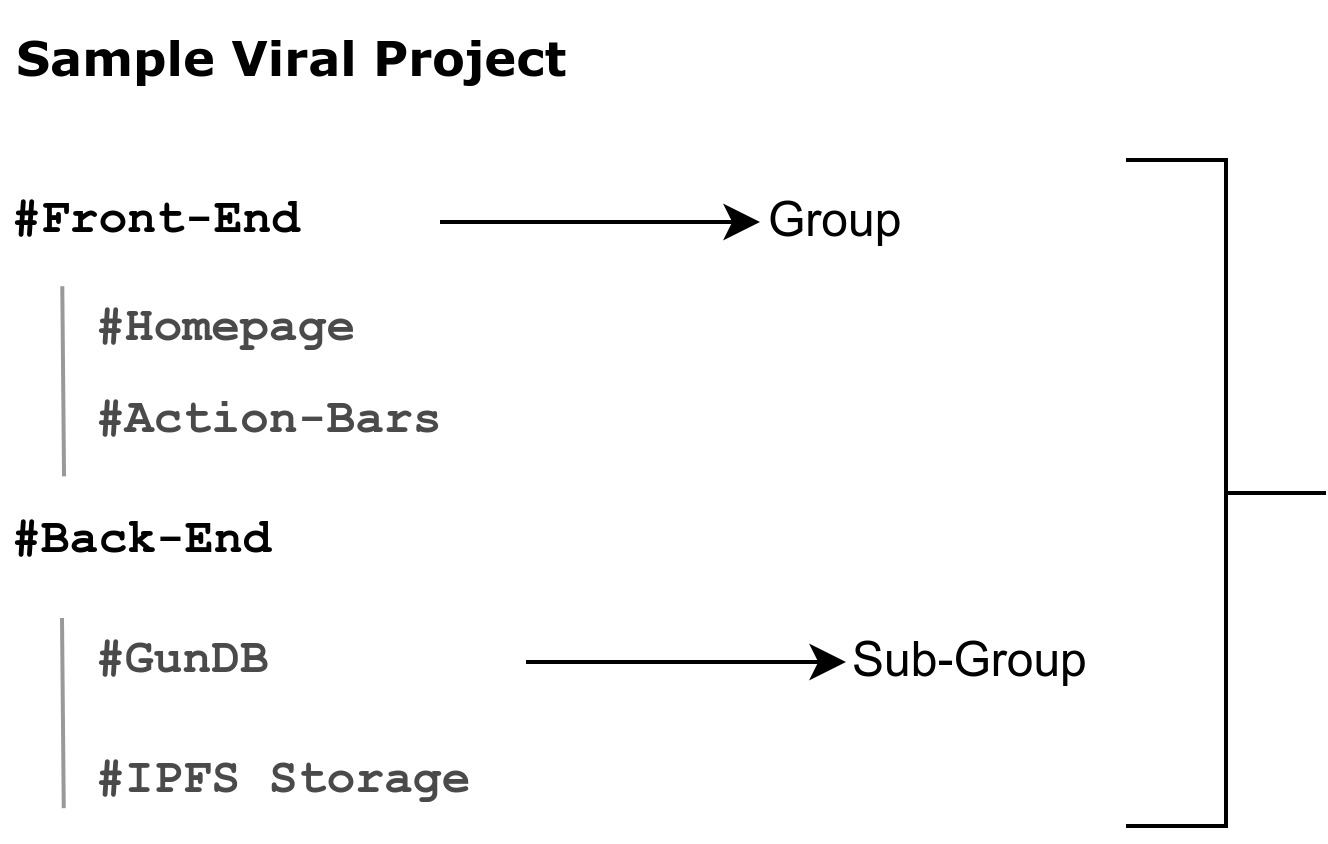
\includegraphics[width=9cm]{chat-community}
\caption{Chat Communities}
\end{center}
\end{figure}

The Workspace is divided by chat groups and sub-groups for communication that represents a commitee of developers working on a certain sector in the repository. Developers can able to post messages, review code in terms of series of communications, conduct private chats, make group/sub-group video meetings and more features which will be updated by the developers themselves on how they would want the environment to be.\\

\textbf{Project Feed \& Shout-outs}\\

The Project Feed is similar to a social media news feed which contains all the successful pull/merge requests by various Public Developers on specific projects. Each Project contains seperate feed where registered developers (who has shout-out privileges) can able to appreciate the contributions that can result in larger reward allocation for a specific contribution. Only the developers currently working on the project can able to shout-out for the inside circle of developers. The feed will be refreshed every 24 hours at 2.00 AM UTC to provide equal time for all the posts to receive shout-outs. The time-line of a pull-request is as follows
\begin{itemize}[wide, labelwidth=!, labelindent=0pt]
\item Merge requests by Public Developers will be reviewed and if conflicts, resolved by the collaborators
\item After the merge request is successful the commits will be made to the beta-branch in the project repository and a post will be scheduled to the project feed at 2.00 AM UTC feed
\item This post will include the developer's VNS (viral) username, git-hub's username and the pull-requet's title, description, snapshot-link, etc.
\item Every pending post will be scheduled on 2.00 AM UTC to provide a equal time period for all the developers to  receive shout-outs from various developers that aids in larger rewards. 
\end{itemize}

\begin{figure}[H]
\begin{center}
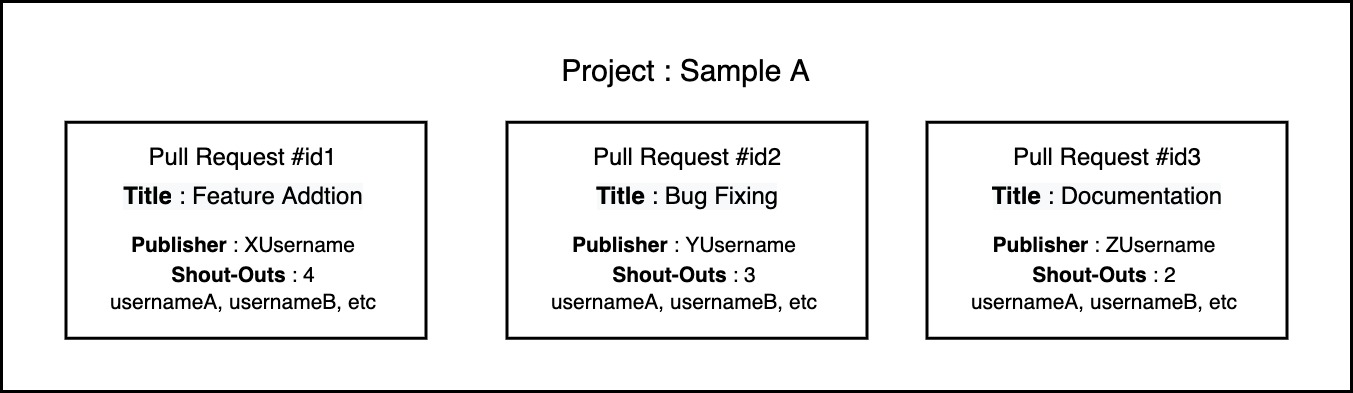
\includegraphics[width=8cm]{post-dev}
\caption{Merge/Pull Requests Post in Project's Feed}
\end{center}
\end{figure}



\textbf{Project Collaborators for Conflict Resolutions}\\

\begin{figure}[H]
\begin{center}
\begin{forest}
  forked edges,
  for tree={edge+={-Latex}},
  [Viral Developers
  	[Private Collaborators]
  	[Public Developers]
  ]
\end{forest}
\end{center}
\end{figure}

Private Collaborators and Public Developers work together to develop, make changes and bring a better beta-application. Both are rewarded for their contribution to the Projects that are run by Viral. Being a collaborator, in a viral project repository you can read (pull) the contents of the repository and write (push) changes to the repository without administrator permissions. Collaborators on existing projects are initialized by Viral Foundation which will be frequently updated by taking top developers working on the current project. Collaborators resolve conflicts on merge requests and update the beta repository accordingly for further releases of the updated application. Collaborators sole purpose is to review the pull/merge requests, resolve conflicts and merge the code. The reward allocation for developers are as follows
\begin{itemize}[wide, labelwidth=!, labelindent=0pt]
\item \textbf{No Conflict - Rewards} : 5\% Collaborator, 90\% Public Developer
\item \textbf{Conflict - Rewards} : 15\% Collaborator, 85\% Public Developer
\end{itemize}

\begin{figure}[H]
\begin{center}
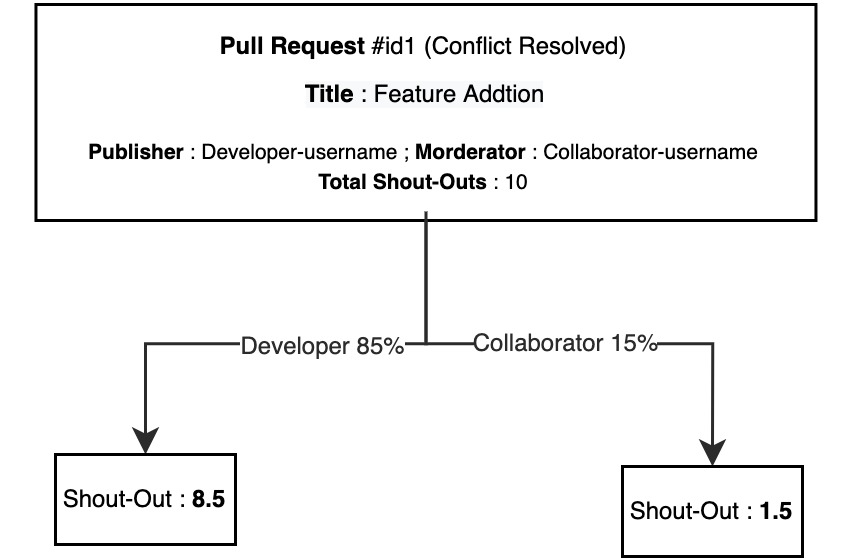
\includegraphics[width=8cm]{dev-reward-distribution}
\caption{Conflict Resolve Collaborator Reward Allocation}
\end{center}
\end{figure}

To add or remove collaborators to the project Git-hub repository, 51\% of the existing collaborators must hold a anonymous vote to prove that the majority would want to add/expel a certain individual from the project.\\
 
\textbf{Rewards for Development}\\

The rewards are based on democratic voting where every developer will have their own project feed to appreciate the work of other developers. There will be an engagement feature to "Shout-out" the contribution they've merged to the code repository. After a developer makes a commitment to the repository by pushing his/her code and after the merge, their work will be posted on to the project's main feed. All posts will be visible for a span of 24 hours 2.00 AM UTC to 2.00 AM UTC, the amount of shout-outs received by the developers on all the projects will be taken to segregate the amount of rewards per developer. Every post will be treated equally where higher the shout-outs higher the rewards. This typically makes a partition of a larger portion of rewards allocated to a bigger developement community project where smaller projects receive only considerable amount of rewards. Refer Rewards section for detailed information on the segregation of total revenue separated for developers.\\


\textbf{New Project Proposals}\\

One of the prominent advantages of Viral's POSI- Paid Open Source Initiative is that creative developers will come up new ideas and significant features which will be annexed to the viral social media application, child platforms or the blockchain environment. These ideas usually in other open-source projects is left out openly where the bootstrapper (developer) will eventually start-up the developement and will carried by other public developers that will result in developers abandoning the project, leaving it's code vulnerable (not updated frequently) due to various factors such as finance, time allocation, work-load.  New projects will be financed by the Viral DAO and will be paid accordingly for every merge request by the public developers to the project repository. Application for financing the projects can be applied by creating a proposal in the governance portal of the Viral DAO platform which will be explained vividly in the Governance section of the Whitepaper. The bootstrappers of the new projects shall request to submit a whitepaper explaining the technical information of the project and the financing rounds information by which a vote will be conducted and the funds will be sent from the Viral-DAO Tresury. Commisions or profit taken from the solutions offered by the developers should allocate a certain portion to the Global Reward Pool. \\

\textbf{Security Bounties}\\

Apart from developer rewards, a certain percentage from the global reward pool is allocated for security bounties which will increases the chances of secure vulnerable-less applications. The shout-outs can be given by all the developers under a certain project for maximizing the amount of reward allocation.\\

\textbf{Other Sections in Dev-Space}
\begin{enumerate}[wide, labelwidth=!, labelindent=0pt]
\item \textbf{Bugs Feed} : Section specifically allocated to see user bug reports experienced in the project's stable release application.
\item \textbf{User Requests} : Users can directly request the project developers for a feature additions or other development ideas from which developers can get neccessary ideas for effective user-expected development.
\end{enumerate}

\textbf{Project Repository Lisencing}\\

\section{\textbf{Influencer-Ad Platform}}

Mainstream modern-advertisement focusses on targeting social media users by running campaigns collaborating between brand and influencers. It takes the idea of celebrity endorsement and places it into a modern-day content-driven marketing campaign. This type of marketing doesn't only involves celebrities but popular content creators who have an enthusiastic audience. Influencers can be anyone anywhere but what separates them from a amateur creators is their large following. Some will have hundreds of thousands, some even millions, brands do care their reputation build around the specific industry that they are looking for i.e, Fashion, Comedy, Sports. They are the people who make engaging contents, share the best pictures, entertain their viewers, run exciting discussions across social platforms on their own specialized topics. From a smaller market size of \$1.6 billion in 2016 it rose to a figure of \$13.8 billion industry in which for every \$1 spent businesses receive purchases worth \$5.78 from all over the world giving an ROI (Return of Investment) of 500\%. About 1360+ Influencer marketing focused platforms and agencies entered the market in the last 5 years alone.\\

Viral Influencer Ad-Platform is a place where influencers get connected with brands and businesses under specific requirements to place paid-ads by determining per-impression rates where Content creators can post brand ads under specific categories such as impressions, engagement, link clicks, etc so brands can purchase with the trust of the blockchain. After the promises of the gig are achieved the payment will be released to the influencers. This effectively reduces the unwanted issues regarding promised results. Viral will be tapping the potential of influencer marketing by running ads through popular content creators. We want to effectively eliminate the excess process of a business to find influencers, contact, fix, transfer amount, etc into a simple user-friendly platform where it can
\begin{itemize}[wide, labelwidth=!, labelindent=0pt]
\item Find tailored Influencers with advanced search algorithm
\item Payment using Viral Pay and multiple available tokens
\item Check Realtime-statistics of the ad
\end{itemize}

\textbf{Influencers}\\

Businesses looking for influencers for their next ad-campaign shall look in terms of followers count on a specific profile where larger brands involve bigger influencers ($\geq$ million followers) and medium enterprises involve smaller influencers ($\leq$ million followers). For seamless results in the Viral Influencer Platform the creators are categorized into several categories according to their followers count

\begin{figure*}
\begin{center}
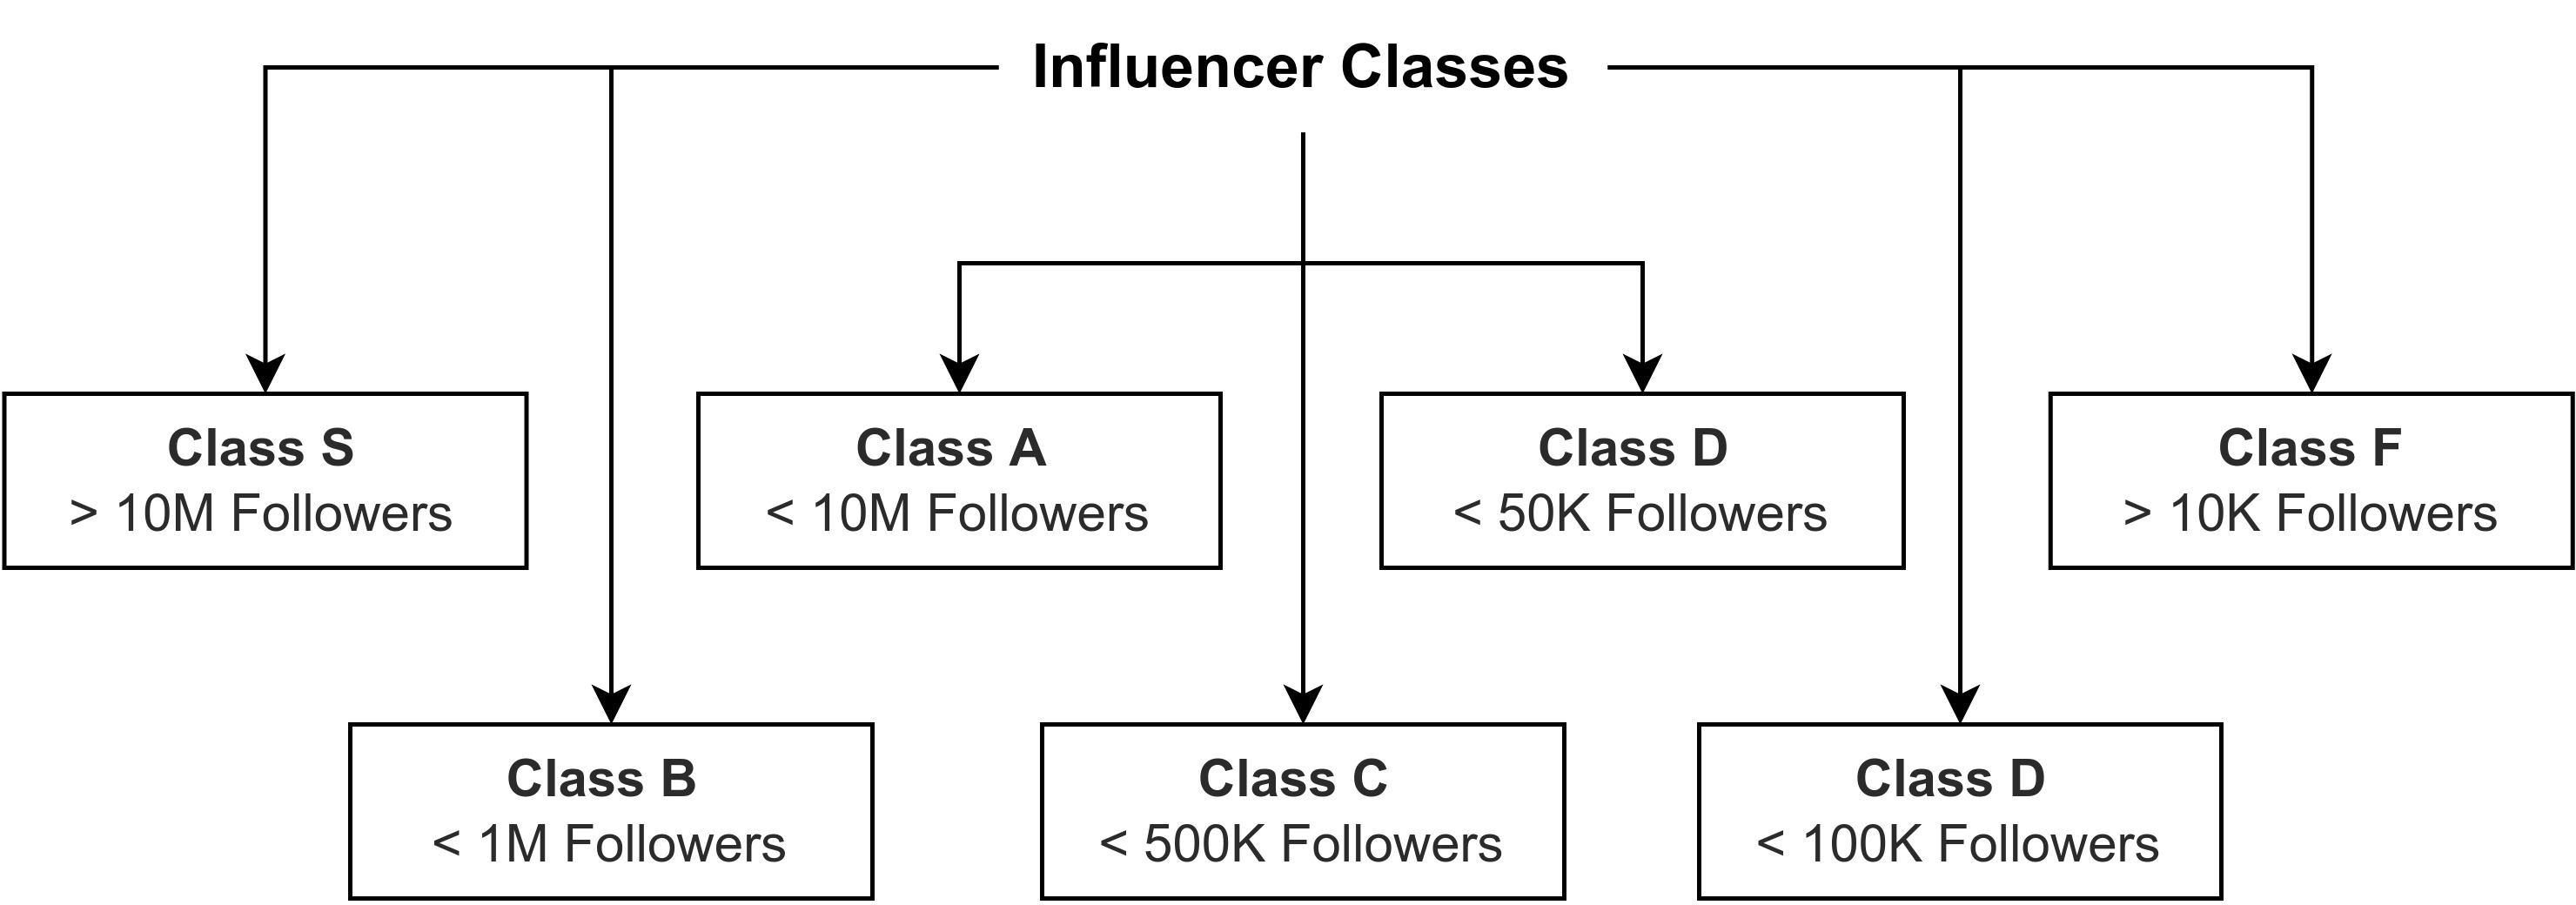
\includegraphics[width=12cm]{influencer-class}
\end{center}
\end{figure*}

A minimum follower count (1K) and a daily impression count is required for signing up in the Viral Influencer Program. Influencers shall provide their per-impression rates on their profiles. Their daily, hourly impression counts are taken into account to display brands and businesses expected ad-result in a certain time period, etc. Influencers can post their per-impression rate on promising certain ad-result for the ad-buyers in easy simple steps. Elite influencers fall onto the category of Class X will be billing higher rates per-impression where smaller Classes will be billing lower rates per-impression. \\

Each Influencer will be classified into niche category. Hashtags of recent posts are taken into account to decide the percentage of posts that is inclined towards a certain category. Sub-categories are also determined for brands to filter and select the best influencer around their target price and ad-performance. Interests of audiences are not taken into any account as Viral is free of data collection systems where the influencer's categories are determined by hastags of recent posts, similarly the influencer can alter his audience interests manually using his/her dashboard.\\

\textbf{Advertising Cost Models}\\

Advertising using Viral Influencer Platform is economic and a better substitution against targeted-ads by social platforms like Facebook, Instagram, Twitter that relies heavily on tracking user's interest to provide them targeted ads. While Platform ads are done aside, the advent of Influencer ads posses more market and provides better ROI and results for the businesses. Viral Influencer Advertising cost depends on various cost models that can be chosen by influencers which is suitable for advertisements. The Models are
\begin{enumerate}[wide, labelwidth=!, labelindent=0pt]
\item \textbf{PPV} : Pay Per-Thousand Views
\item \textbf{PPC} : Pay Per-Conversion
\item \textbf{PPD} : Pay Per-Day
\item \textbf{PPP} : Pay Per-Post
\end{enumerate}


\textbf{Pay-Per-Thousand Views}\\

PPV is the default pricing option in the Viral Influencer Platform. It is one of the key-metrics of influencer ads which defines "Total Cost per 1,000 views from an ad post" which is used to understand the pricing, ad's effectiveness and performance. Views means total number of times the post is displayed to the users. Views will contain if a single user watches multiple times the same ad post. Similarly additional metrics are given such as
\begin{itemize}[wide, labelwidth=!, labelindent=0pt]
\item \textbf{Outreach} : To determine the number of users the ad have reached excluding multiple views of a single user.
\item \textbf{Conversions} : To determine the number of conversions such as link clicks that is provided on the caption, etc. Conversion doesn't includes profile visits of the influencer.
\end{itemize}

The PPV cost of influencers are provided upon registration and will be available for brands and businesses to research for their advertisements. Currently targeted advertisements by various centralized social entities are charging \$7 per thousand impressions, viral influencer platform aims to achieve more affordable standard rates over centralized solutions tailoring for each influencer that suits their reputation in the following industry.\\

\textbf{Pay-Per-Conversion}\\

Conversions are suitably links or tags which gets clicked by the user that may funnel them into further actions. PPC ads are used to drive traffic to websites, brand-pages, etc. The advertiser (influencer) charges a fee every time a link is clicked through the ad-post. Essentially PPC is the way of buying visits to your preferred page/website, rather than attempting to earn those visits organically. Influencers can provide their Pay-Per-Conversion rates to their profile which will attract brands to partner and advertise their content in an efficient manner.\\ 

\textbf{Pay-Per-Day}\\

Influencers usually charge payments for running brand ads according to the amount of days the ad-post will reside on their page. Different influencers such as informative pages, meme pages, niche pages attract businesses to pay them for ad posts that will be ran for a certain amount of days receiving quality amount of impressions and conversions to the brand. Influencers can provide their Pay-Per-Day rates to notify brands the best rates for advertising to their followers and new visitors.\\

\textbf{Pay-Per-Post}\\

Pay-Per Post is a simple, direct advertising by influencers, celebrities and models to publish branded-ads by pricing it per post. Influencers can provide their per-post price to directly display how much the cost would be to deliver branded-ads to quality like-minded followers and fans. This direct advertising is preferred by most bigger brands as it costs higher and the ROI is better in terms of other advertisement models.\\

\textbf{Ad-campaign}\\

\begin{figure}[H]
\begin{center}
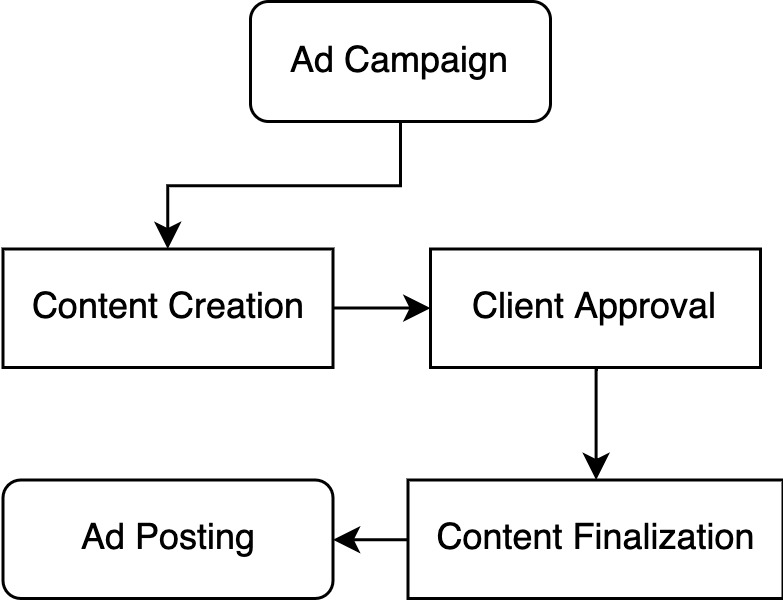
\includegraphics[width=5cm]{ad-flow}
\caption{Ad-Campaign Flow}
\end{center}
\end{figure}

Each Ad-Campaign comprises of several funnels to give the best advert without compromising quality. The Campaign starts-off with choosing the right set of influencers using search filters and sorting algorithms. After the selection of influencers the initial payment will be done to pass on the campaign's status to content creation, where the influencer shall provide production ready or draft content for the client's approval. After rigorous checking and updating the content, the ad is finalized and published. The Payment will be withdrawn according the advertisement-model from the client's ad-fund contract. Each step is clearly explained in the following paragraphs.\\ 

\begin{figure}[H]
\begin{center}
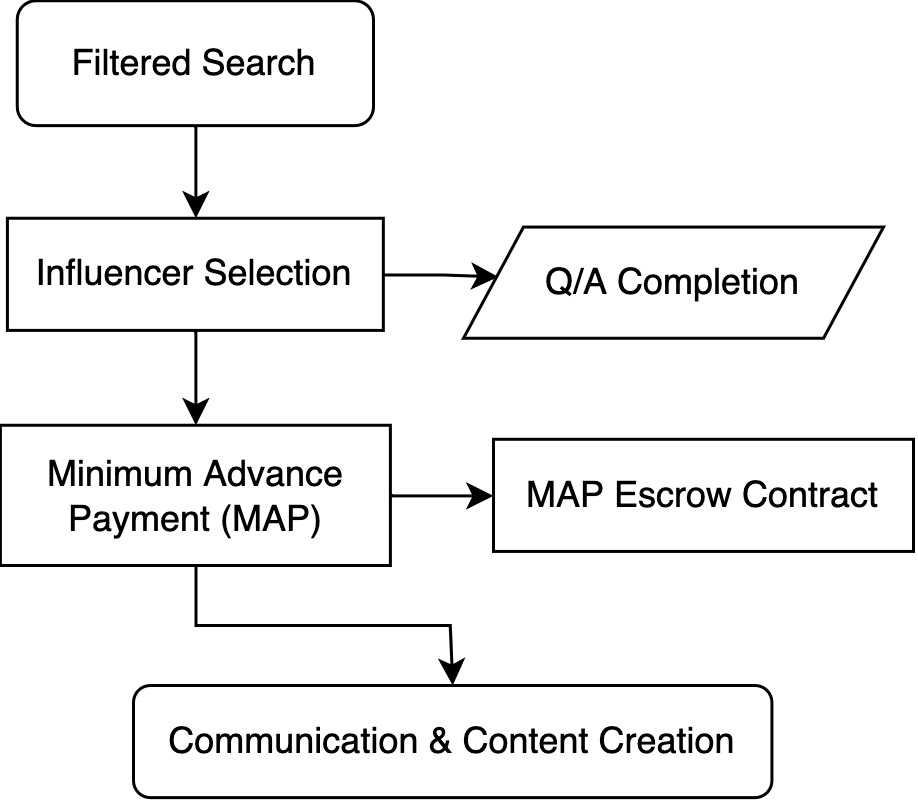
\includegraphics[width=6cm]{ad-selection}
\caption{Influencer Selection \& Initializing Payment}
\end{center}
\end{figure}

Searching Influencers on Viral Influencer Platform is better in terms of finding a targeted niche content creator for best price and ROI. The platform will provide Brands and Businesses looking for promoting their content on Viral where they can narrow their search to their expected influencers. This makes it easy for individuals and businesses without worrying about the research.Some of the filters we are exploring are
\begin{itemize}[wide, labelwidth=!, labelindent=0pt]
\item Niche Category (Eg: Food)
\item Follower count (Eg: more than 1M followers)
\item Account Age (Eg: 6 months)
\item Daily Impression (Eg: 257k views)
\item Country (Eg: Canada)
\item Reviews and Ratings
\item Price-Per Thousand Views (Eg: \$1.23)
\item Price-Per Conversion (Eg: \$2.5)
\item Price-Per Post (Eg: \$360)
\item Price-Per Day (Eg: \$75)
\end{itemize}

The Influencers are selected and white-listed for further decisions. After a specific/group of influencer is chosen the further proceeding is to fill a Q/A session that consists of default and specified question that help the influencer to tailor up the ad in terms of directly communicating the brand or endorsing the product in a natural and engaging way. An Example Q/A given below
\begin{enumerate}[wide, labelwidth=!, labelindent=0pt]
\item Brand Name and External Links
\item Product or Service Short Brief
\item Video Links
\item Ad-Description
\end{enumerate}
After the Q/A is completed the client shall be reverted to pay a Minimum Advance Payment. MAP is a refundable escrow payment allocated for subsidizing the creators in an account of cancellation by the client for an un-fulfilled production of the branded-content. To reduce spamming influencers, the MAP amount is paid and confirmed to start a communication between the client \& the influencer. The MAP amount will be provided by the influencer for a safer payment procedure. Once the MAP is paid, the Q/A and the client details will be sent to the influencer directly where he/she can directly start communicating for the creation of draft-ad.

\begin{figure}[H]
\begin{center}
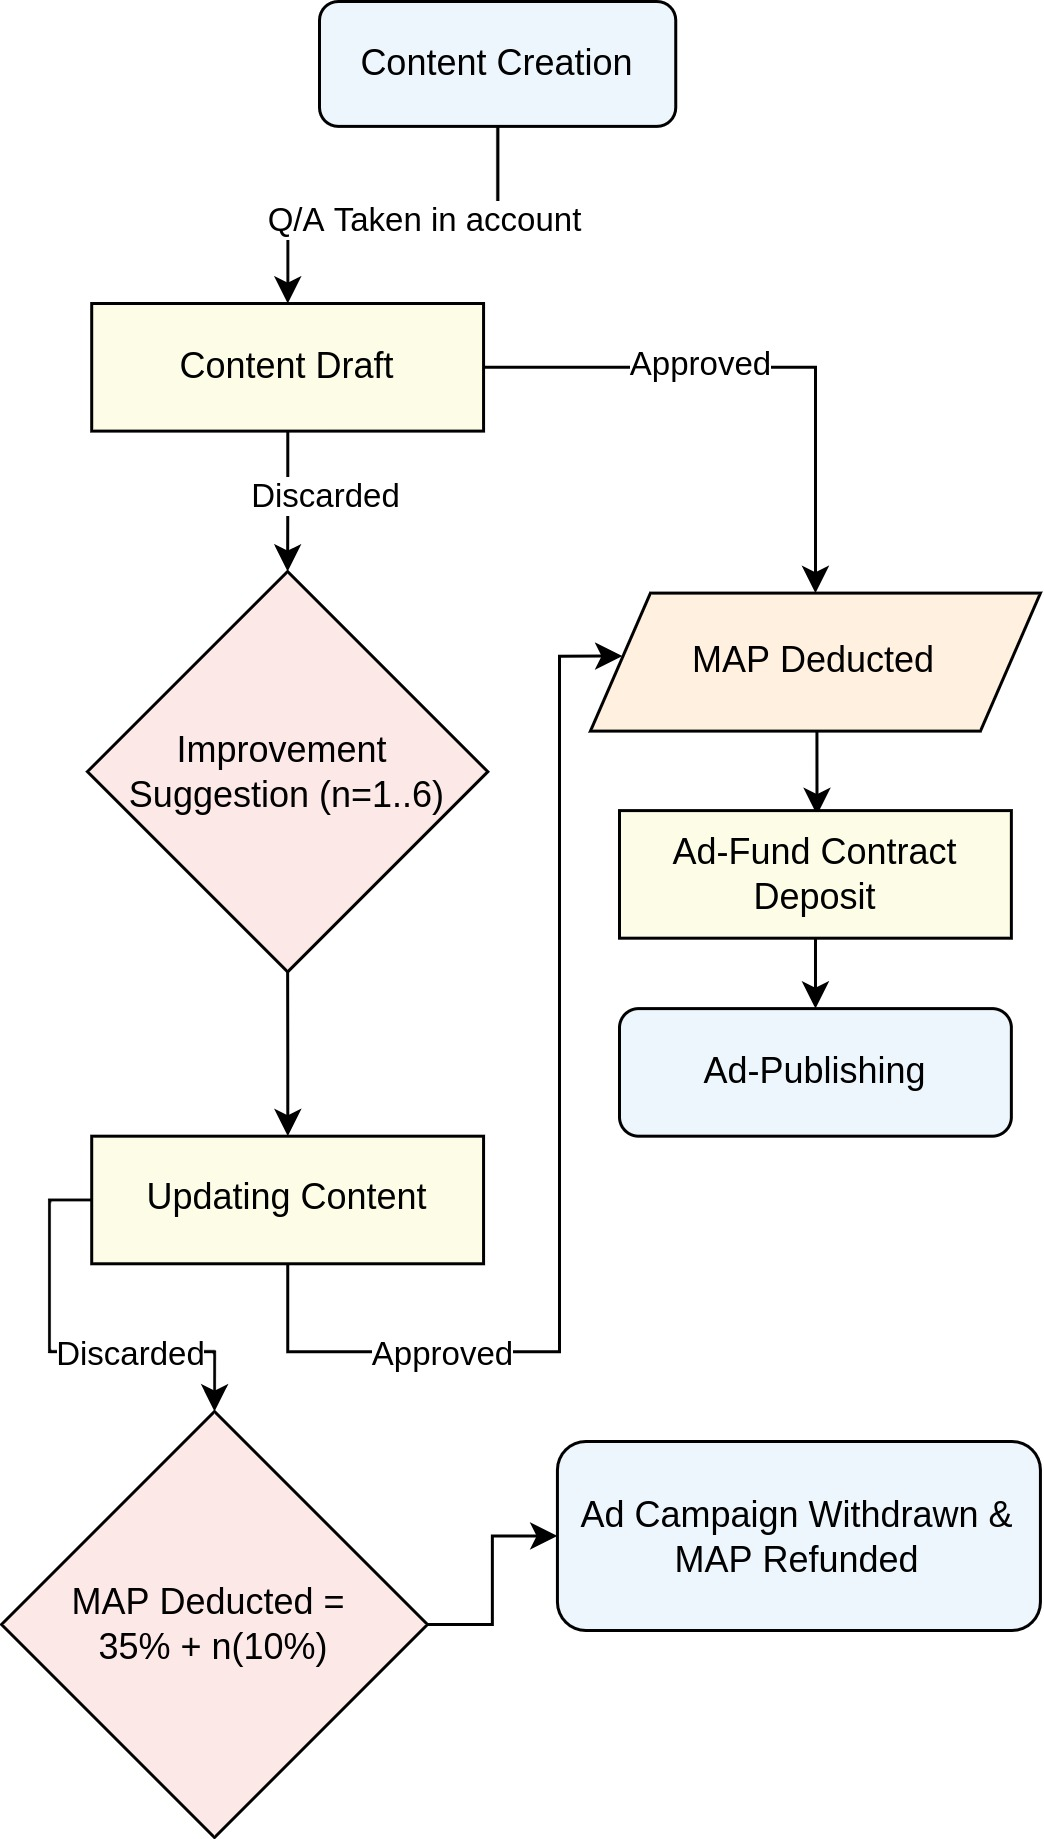
\includegraphics[width=6cm]{ad-content}
\caption{Content Creation \& Cancellation}
\end{center}
\end{figure}

Every Content creation starts off-with studying the Q/A and the client's needs regarding how the campaign should sound. The Influencer then starts off with producing the media content and sending the first draft to the client through the influencer portal. The Client goes through the draft and suggests improvement or changes in the content if the client want to. The Improvement suggestions are limited to a maximum of 6, to avoid spamming the creator with multiple iteration of changes to the content. If the content is not approved for a sixth consecutive time, the MAP is deducted and the Ad-Campaign is withdrawn. A subsidiary fee deducted from the MAP will be sent to the influencer for aiding in creating the content for the client. When the client opts to withdraw the ad-campaign the MAP (Minimum Advance Payment) percentage to be deducted will be decided upon the number of drafts the creator provided i.e., $x=35\%+n(10\%)$ where 35\% is the subsidiary fee for the influencer for the first draft and the n denotes the number of improvement suggestions made by the client. If the content is approved before the 6$^{th}$ draft, the MAP is deducted and the Ad will be prepared to publish. An Ad-Fund Contract will be assigned for the client to deposit funds for running the campaign where the funds shall be withdrawn periodically according to the advertisement model the client chooses i.e., PPV - Pay per-Thousand Views, PPD - Pay per-Post, etc.

\begin{equation}
MAP\:Deducted=35\%+n(10\%)
\end{equation}

\begin{figure*}
\begin{center}
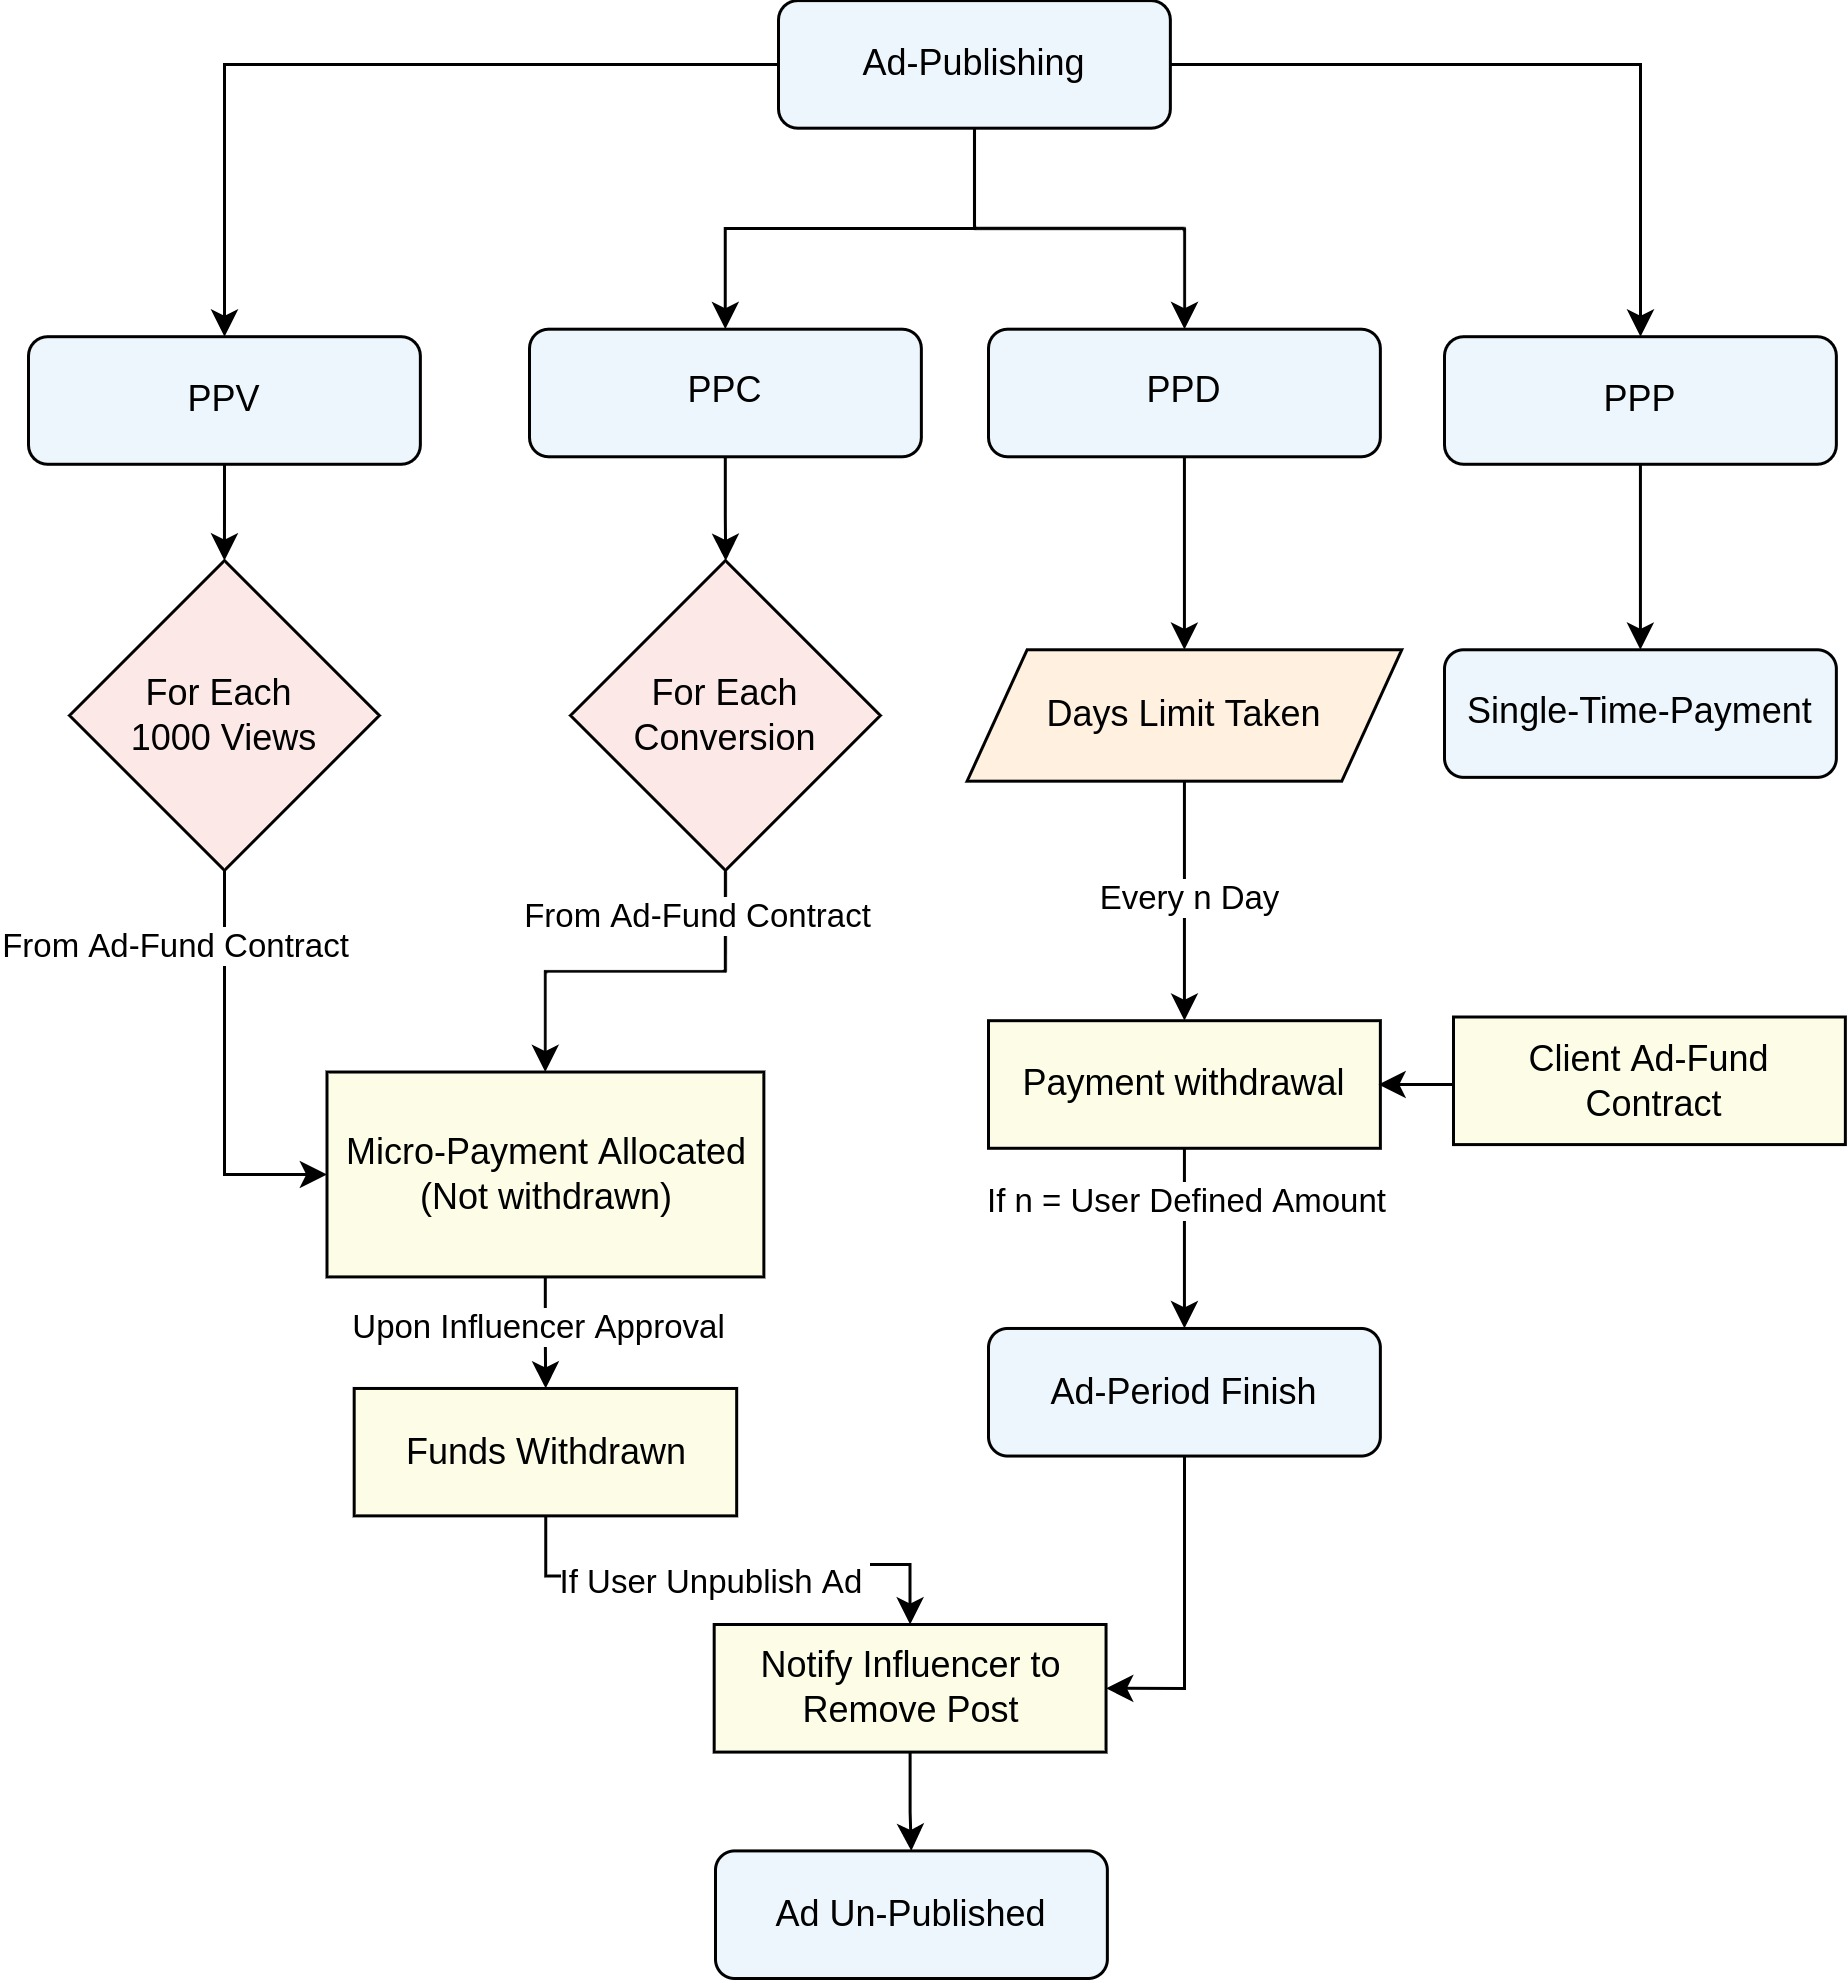
\includegraphics[width=11cm]{ad-publish}
\caption{Ad-Publishing over various payment models}
\end{center}
\end{figure*}

The Ad is published after the finalization by the client. The Payment is taken periodically according to the ad-model the client opted for. The Pay-per Thousand Views (PPV) model allocates micro-payments for the influencer for every 1000 views reached, the view-feed is taken directly from the viral application and provided onto the ad-fund contract directly through decentralized oracles. The Payments aren't withdrawn from the Ad-Fund Contract rather it is allocated to the influencer's public address similar to "Viral Reward Pool" inside the smart contract itself. The Influencer can withdraw all the allocated tokens from all the ad-campaigns upon signing the transaction via his viral wallet. This way micro-transaction dusts can be eliminated batching all transactions into a single macro-payment. \\

Similarly the Pay-per Conversion allocates funds inside the Ad-Fund Contract for each conversion. The Pay-per Day allocates funds for every 24 hours since the ad-published. When the ad-period finishes a notification is sent to the influencer to un-publish the advertisement. The Pay-per Post directly takes a single payment from the Ad-Fund Contract and directly sends the tokens to the Influencer Wallet.\\

\textbf{Periodic Allocation}\\

\begin{figure}[H]
\begin{center}
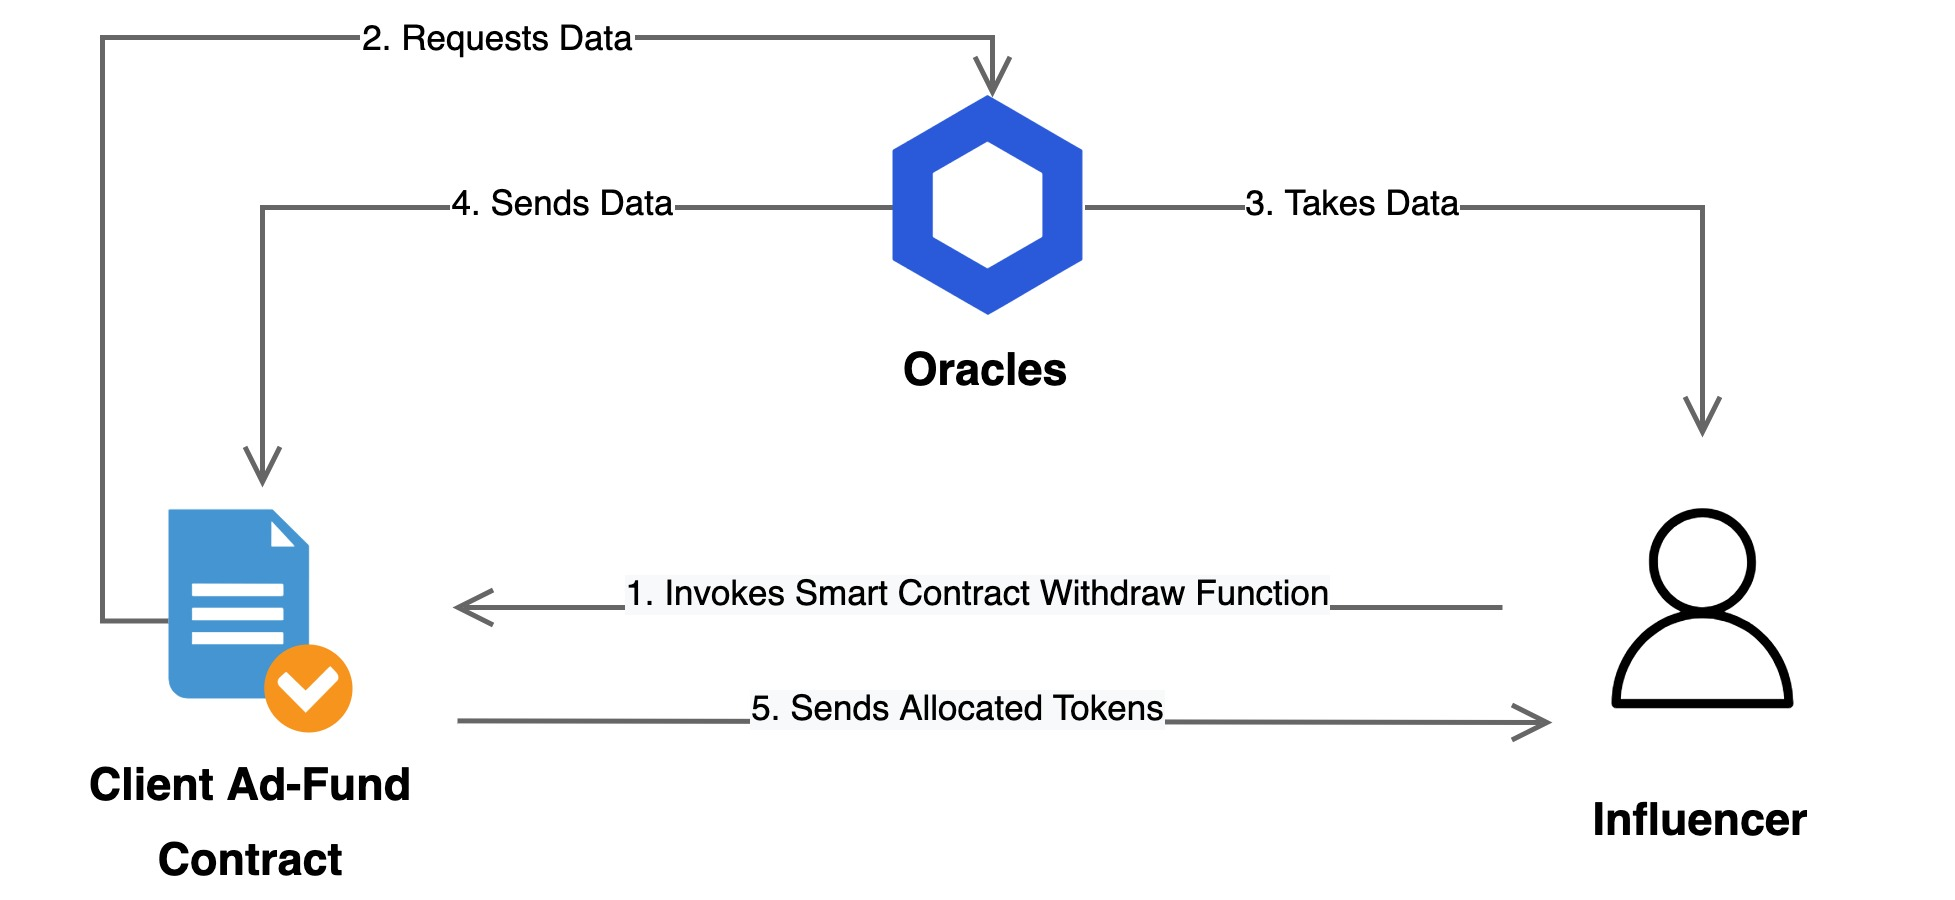
\includegraphics[width=8cm]{periodic-allocation}
\caption{Influencer Withdrawal of Funds}
\end{center}
\end{figure}

Periodic Allocation refers to the manual withdrawal function called by the influencer on all the running ad-campaigns to withdraw the allocated tokens for publishing the advertisement on the influencer's viral social account. Withdrawing funds works by taking the necessary data required for  calculating the allocation of funds and withdrawing it directly to the influencer's viral wallet- similar to centralized billing where the billed amount will be auto-debited from the client's credit card to the company, but here directly to the influencer. Every time the influencer opts for withdrawing his/her funds the smart contracts are invoked and the "influencer-withdrawal" function is called.\\

\[Withdrawal\:Insight=Total\:Insight-Last\:Withdrawn\:Insight\]
\[Withdrawal\:Amount=Wuthdrawal\:Insight \times AdModel\:Rate\]
The Ad-Fund Contract fetches the necessary data from a decentralized oracle feed that directly takes the insights of the advertisement i.e., 25 Conversions, 35k Views, etc and calculates the allocation by subtracting the previous allocation from the total allocation e.g., 10,000 total views, Recent withdrawal at 9,500 views, 500 views allocation for now. The recent Insight calculated for the new withdrawal is taken and the exact amount of token withdrawal is determined by the Ad-Fund Contract. After the Ad-is published the advertisement model-rate will be fed to the ad-fund contract thereby reassuring stable rate throughout the entire ad-campaign e.g., \$1.5 per conversion will always be \$1.5 throughout the campaign from which the withdrawal amount is calculated and sent to the influencer's wallet. Payment in multiple-tokens in the Viral Influencer Platform brings a whole new multi-tokenized marketing opportunities around the globe\\

\begin{figure*}
\begin{center}
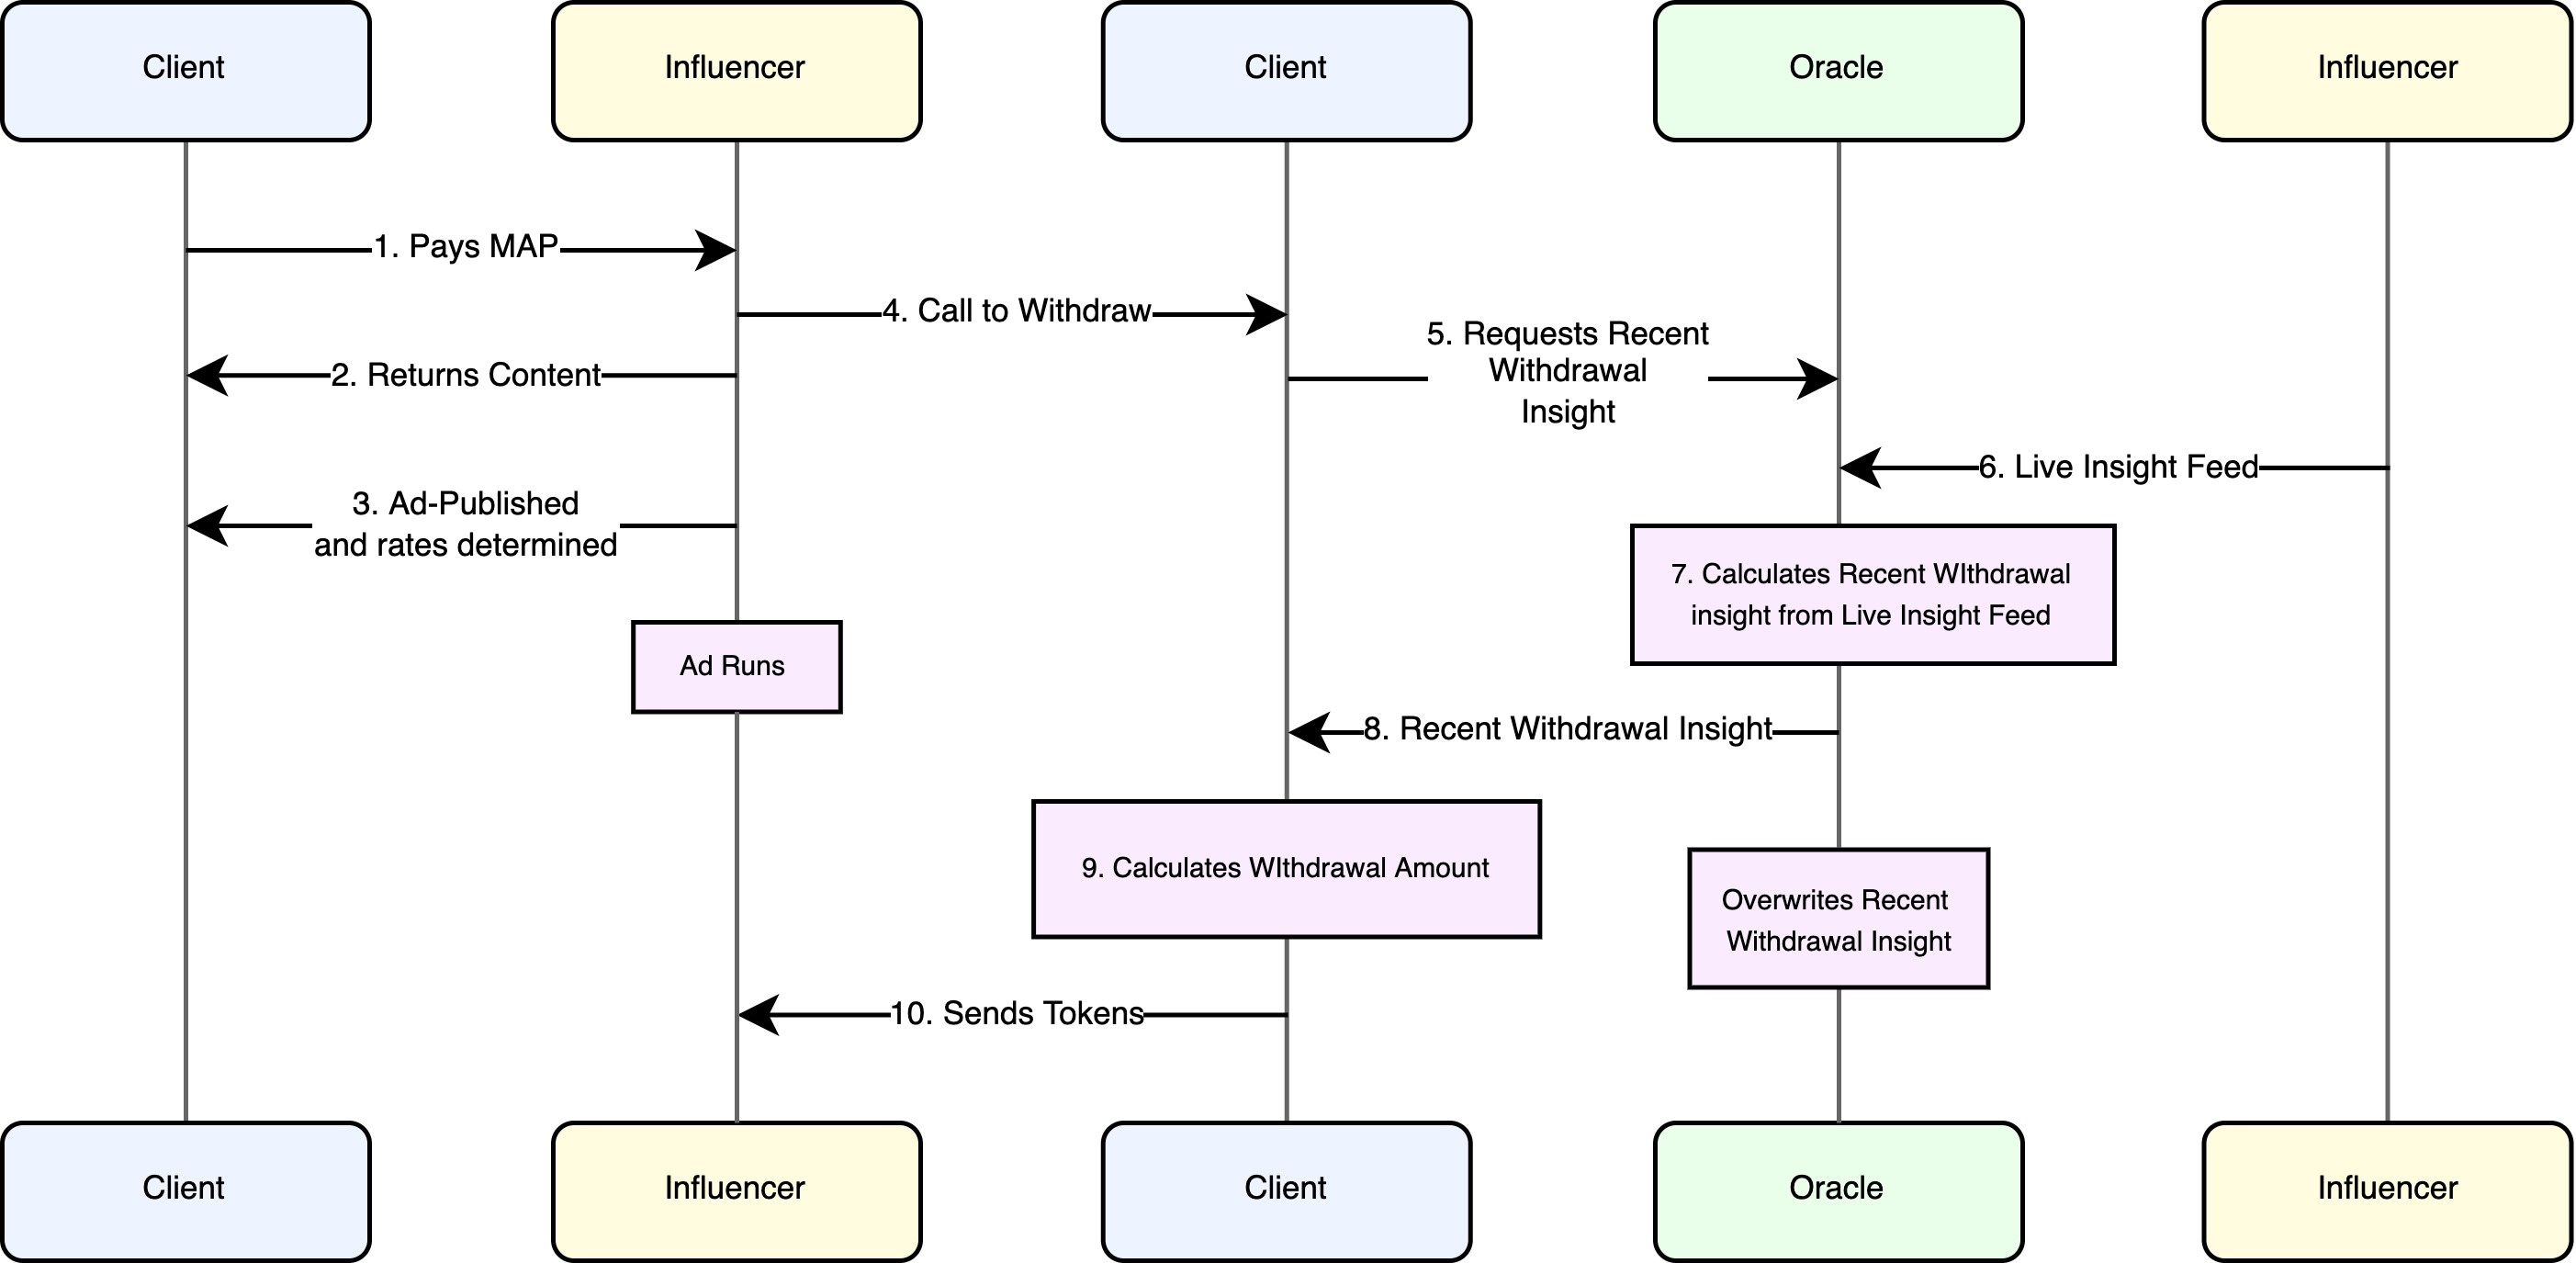
\includegraphics[width=12cm]{periodic-allocation-2}
\caption{Sequence of Withdrawal}
\end{center}
\end{figure*}

\textbf{Fees \& Billing}\\

PPV - Every Withdrawal - 20\%\\


\textbf{Benefits of Viral-Influencer Ads}
\begin{enumerate}[wide, labelwidth=!, labelindent=0pt]
\item \textbf{Pay for proof} : Crypto-based Influencer Platform based on pay for proof concept similar to current social ads which bills clients on the basis of insights.
\item \textbf{Easy Ad-Models} : Pay-per Ad models which is based on Views, Conversions, Days, Post brings whole new opportunities for clients and influencers.
\item \textbf{Multi-Token Payment} : Promotes tokenized economy and benefits building a portfolio of pre-determined receiving tokens for ads.
\item \textbf{Secure Ad-Funds} : Ad-Funds are stored in smart-contracts instead of central custodian banks makes it secure and facilitates autonomous payments with additional signatures.
\item \textbf{Variety of Influencers} : The platform will offer vast influencer options where diversification of single ad-campaign aids to a significant results in higher ROI.
\item \textbf{Simple Communication} : Efficient communication between the client and the influencer throughout the ad-campaign.
\item \textbf{Rookie, Intermediary, Elite Categories} : Supports small, mid and veteran influencer for affordable to top-branded ads.
\item \textbf{Conflict Resolution} : Pre-defined systems like Minimum Advance Payment resolves the sudden cancellation after content production by deducting and sending a subsidiary payment to the influencers.
\item \textbf{Zero Spams} : Hiring Influencers starts-off with providing a Q/A along with a payment that can reduce spamming influencer with offers.
\end{enumerate}
\section{\textbf{Viral Decentralized Ads}}

Intro\\
Current Social Ad Benefits \& Problems\\
Privacy Issues\\
Current Marketing Models \& Cons\\
Basic Overview\\
Concept of Decentralized Privacy Focussed Ads\\
User Opting \& Quality Based\\
Use of Zk-Proofs\\
Technical Overview\\
Cost Models\\
Ad-Areas \& Conversion rates\\
Ad Types\\
Reducing Spams\\
Allocation of Ad-cost\\
Ad-Funds for better targeting\\
\section{\textbf{P2P Exchange}}

Nowadays people want cryptocurrencies without transaction fees, exchange fees, and also without KYC process in an anonymous way. But in order to buy on central exchanges using Fiat-Money, it is not possible without disclosing their personal information and identity cards for Anti-Money-Laundering purposes. Buying cryptocurrencies using fiat money is not possible on Decentralized Exchanges, since it is a platform to swap from one cryptocurrency to another cryptocurrency in a decentralized manner without any centralized order books.\\

This is where P2P exchanges come in. Peer-to-peer refers to the exchange or sharing of information, data, or assets between parties without the involvement of a central authority. These P2P exchanges work on connecting two users nearby around their city, area, who are willing to sell and buy crypto tokens for fiat currencies. Thereby making an agreement of holding the seller's cryptocurrencies in a smart contract to verify sellers and withdraw to buyer until he transfers the fiat-currency funds to the seller and gets confirmed.\\

\textbf{Advantages over Centralized}

\begin{enumerate}[wide, labelwidth=!, labelindent=0pt]
\item Peer-to-peer transactions generally do not require the involved parties to provide identification,  protecting everyone's right to privacy. 
\item P2P exchanges allow the purchase of cryptocurrencies through the regional medium of exchange that the seller opts for (E.g. PayPal, Square, M-Pesa  etc). Viral offers P2P solutions to all countries' local payment methods for the users without any hassles.
\end{enumerate}

\textbf{P2P for Sellers}\\

Seller listing will be initiated by the token seller. The tokens are allocated on a escrow smart contract that will be holding the funds which can be only withdrawn in the account of closing the listing. Non-sensitive information such as City, State, Country shall be provided upon listing which is preferred by buyers for smooth trade of tokens offline. The Regional Payment Methods are selected and the listing is created. The listing consists of Token name, Tokens amount, Payment methods and City.\\

\begin{figure}[H]
\begin{center}
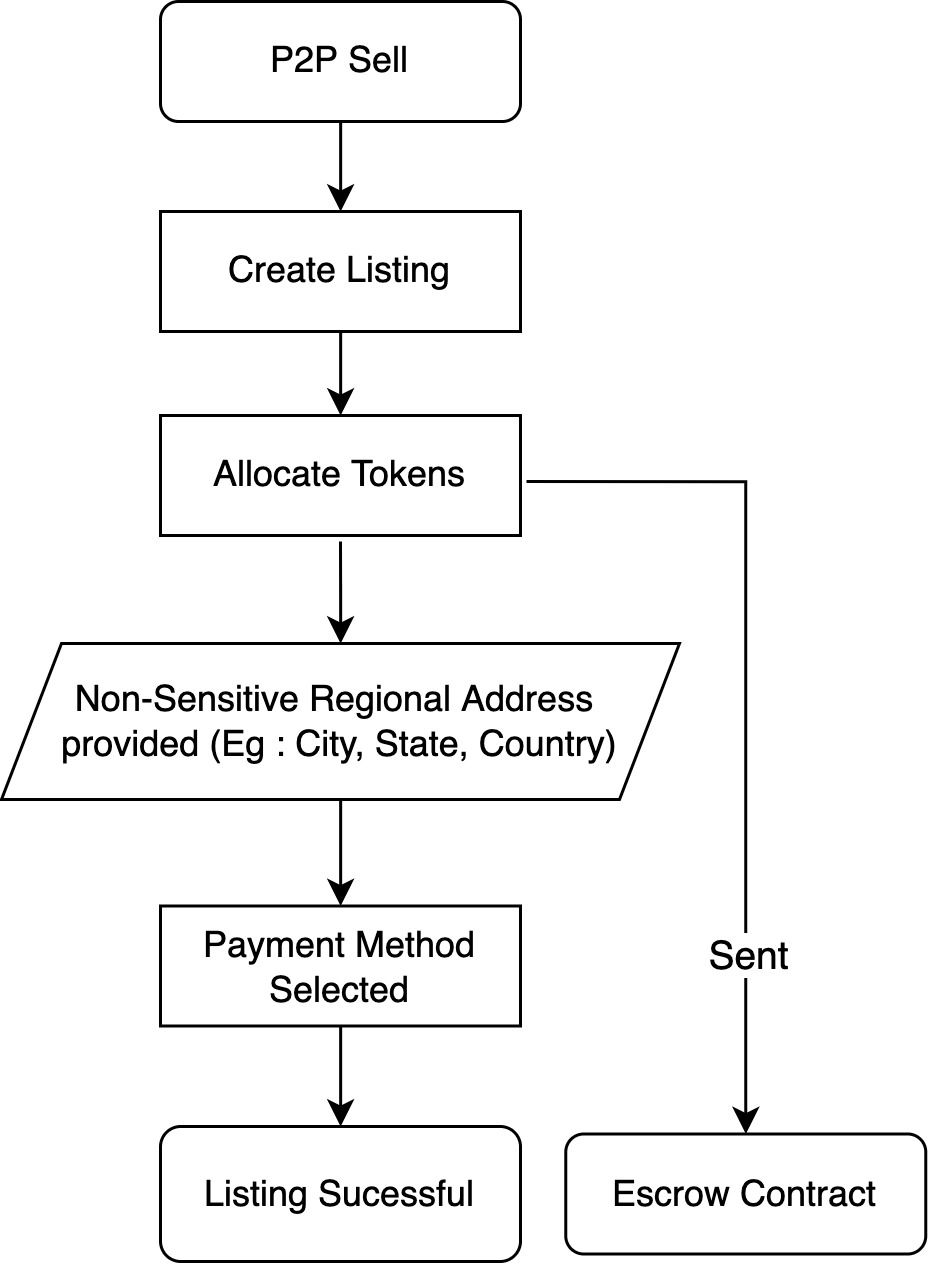
\includegraphics[width=6cm]{p2p-sell}
\caption{Selling Tokens via P2P}
\end{center}
\end{figure}

\begin{lstlisting}[caption={Token Sale Listing}, numbers=none]

	listing id: 02698 {
	
    	"token-id": "vrl",
   		"token-ticker": "VRL",
    	"token-amount": "7289.375",
    	"city" : "Los Angeles"
    	"state" : "California"
    	"escrow-contract-id" : "vy89xfwieug2t8793br9hd2by2dfg"
    	
	}
\end{lstlisting}

\textbf{P2P for Buyers}\\

Users can buy tokens in a secured anonymous manner by connecting with sellers using the P2P Viral Exchange. The Location shall be provided by the buyer to list all the potential seller listing that can be selected upon confirmation by the buyer. The buyer will be immediately connected with the seller by initiating a chat. All the sell listing on the Viral P2P exchange are verified by the escrow smart contract balance which will hold exact value/balance of the listing which offeres a trustless solution for the buyer. After the chat is connected, the seller and buyer shall communicate with each other and provide locations to visit in person or to agree on terms for ssmoother trade without conflicts.\\

The Buyer enters the amount of tokens he would like to buy and the current market price is fetched for the buyer. After the buyers sends the fiat payment, the buyer shall confirm his/her payment. The Seller refers the fiat payment and confirms it. After the confirmation from both parties the contract is revoked and the specified amount of tokens will be sent directly to the buyer's Viral wallet.\\
\begin{figure}[H]
\begin{center}
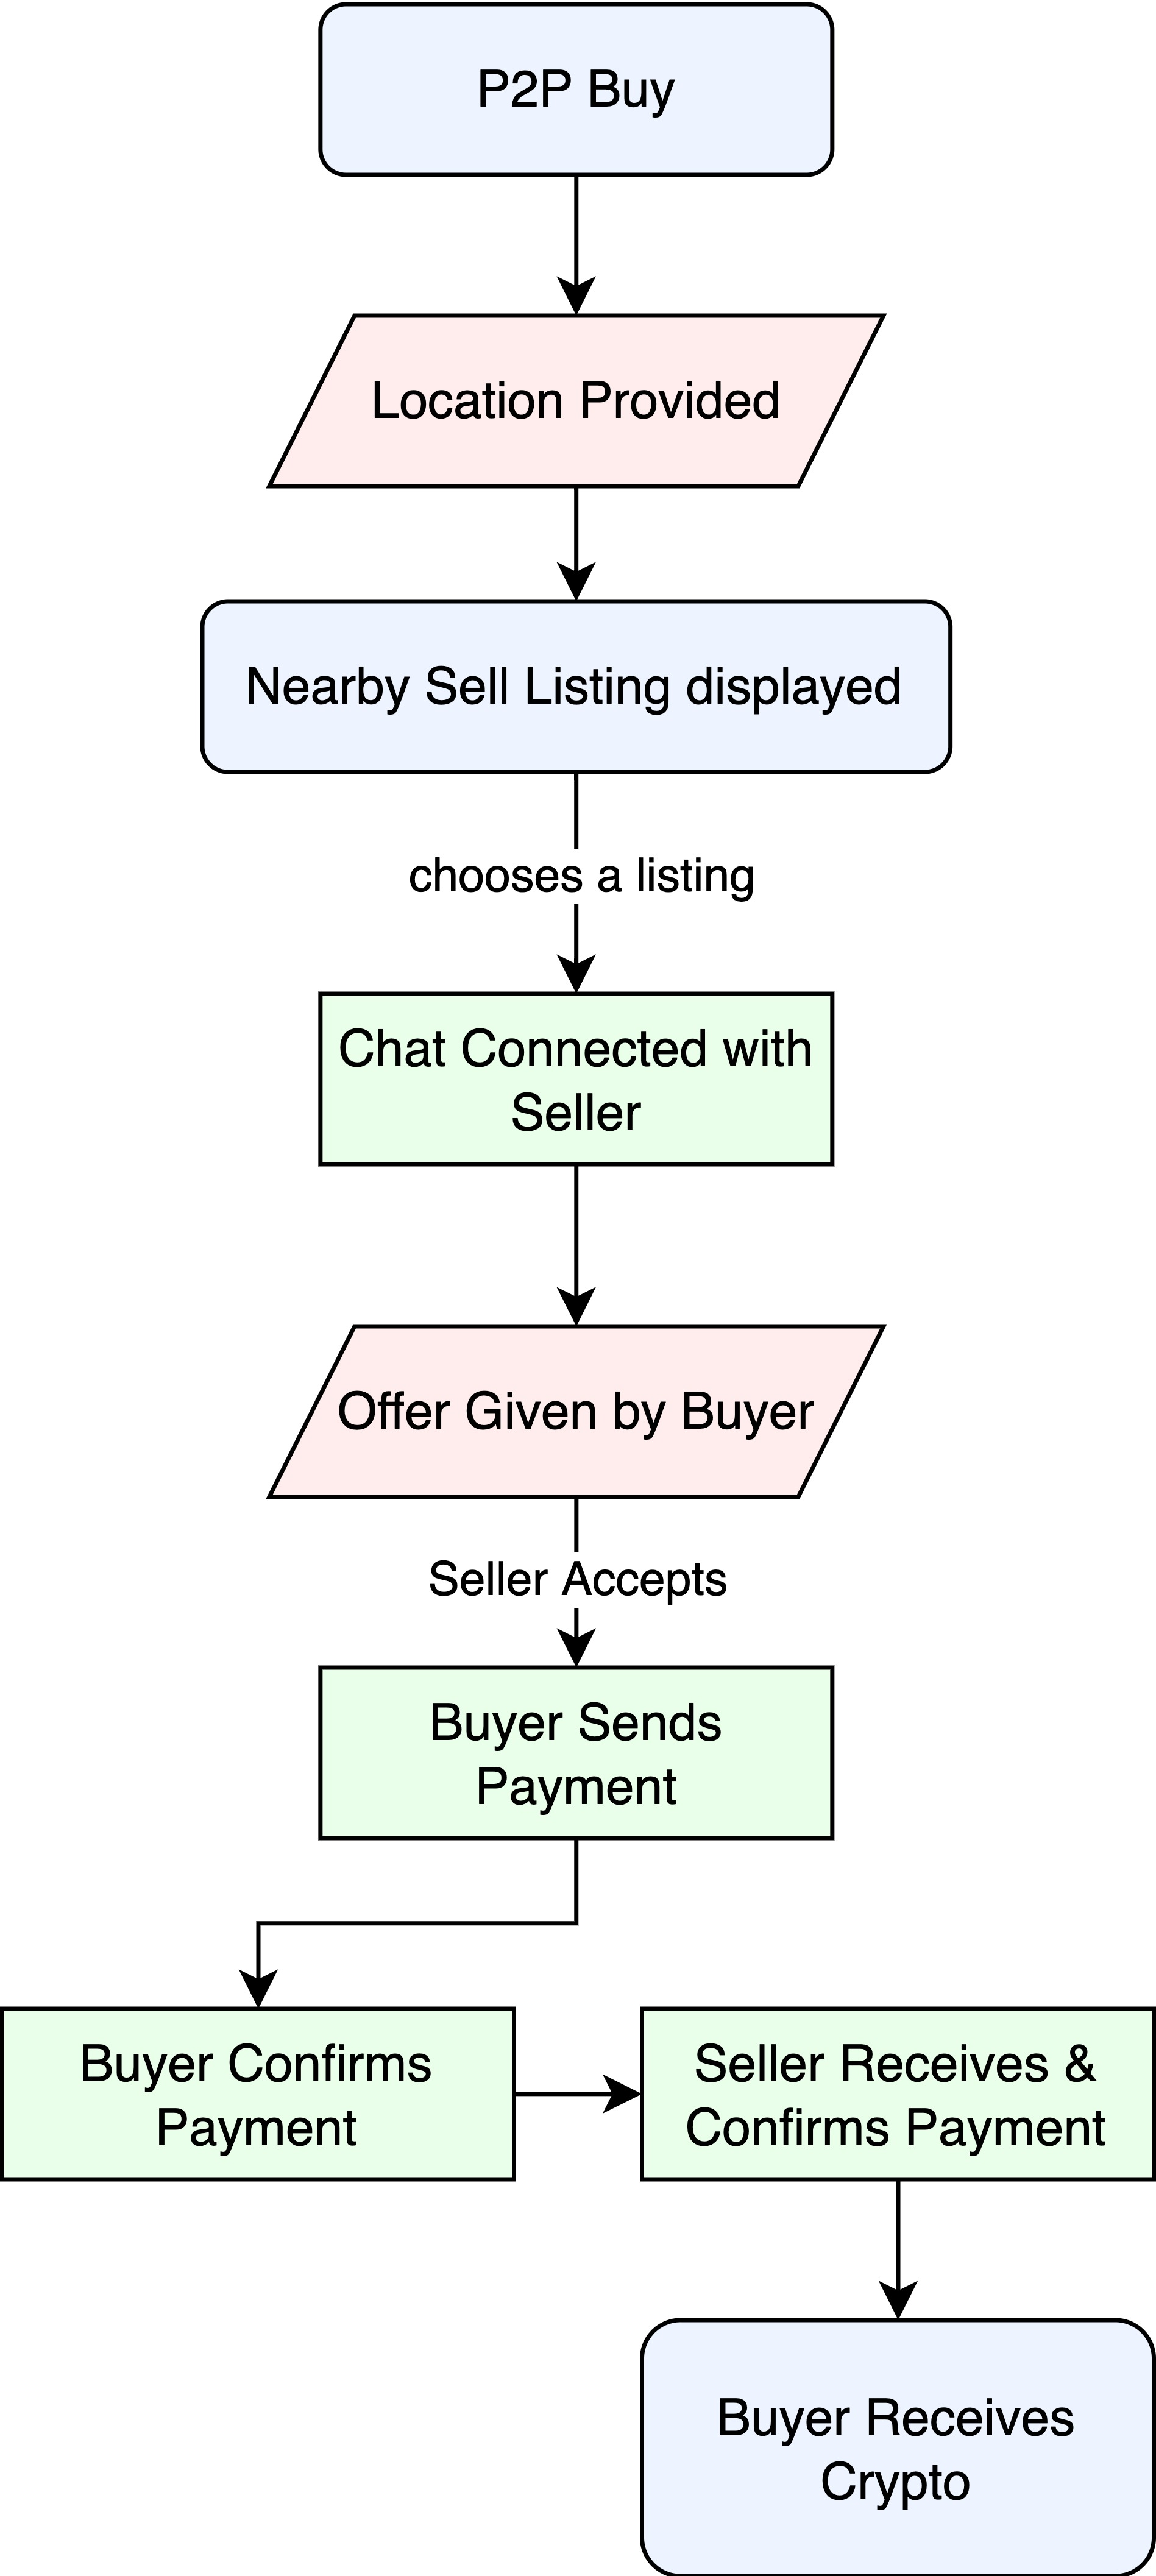
\includegraphics[width=5cm]{p2p-buy}
\caption{Selling Tokens via P2P}
\end{center}
\end{figure}
Our ultimate vision is to develop a decentralized social media without any central authority or a need for a company to run its product, a P2P Exchange will carry out its process of buying and selling Viral Coins for Fiat money. This ensures the trades cannot be banned nor withdrawn no matter what the land rules are.\\
\section{\textbf{Viral Open-Source Distributions}}
Open Source Softwares are copied by individuals and entities apart from the main organization that bootstrapped the original project. The copies are forked, modified, managed and distribued independently resulting in development of a new version or a distribution under the same open-source rules. Apart from different versions of the same software, the core which is built upon will be the same for all the distributions. An Open-source project can have as many distributions adhering with it's license to copy the source-code. For example, the Linux project has given rise to distros like SUSE, Red Hat, Ubuntu, CentOS, and many others. But all Linux distros use the same Linux kernel.\\
Why Viral is Open Source\\
What it attracts\\
What's the Benefit\\
Future of Viral\\
How Revenue Pool works\\
Compensation and Welcoming new distributions\\
Core for new Social Media leveraging Viral's Storage, Blockchain, Child Platforms\\
\section{\textbf{Global Reward Pool}}
To develop a truly decentralized company, the segregation of expenditures and investments should be determined and allocated through an automated smart contract. The profits should be divided across employees - in Viral's case it's volunteers,  investors as dividends, and for further new projects. Viral Rewards are daily rewards allocated to every user on the decentralized platform who contributes towards running the platform. It includes Users, Miners, Volunteers, and DAO Members. Since it is a decentralized platform, it requires no maintenance and authority by a centralized entity. The contribution of every single individual user is needed to run the platform seamlessly. We would be giving out rewards in Viral native tokens and Wrapped tokens of popular cryptocurrencies such as Bitcoin, Ethereum, Solana, etc for all the users who contribute towards running the social and multi-chain platform.\\

The Reward allocation for each user happens through automated smart contracts every day at 2 AM UTC. Viral Rewards are designed in such a way that every single contributor inside the network will get paid for their contribution through a either democratic voting system or mathematically predicted points. These points prediction program will be calculated from off-chain real-time data through decentralized tamper-proof oracles in a secure  manner to ensure fair rewards to each user without any influence, third-party recommendation, or external factors. \\

The 100\% percent of total daily revenue is distributed as \\
\begin{figure}[H]
\begin{center}
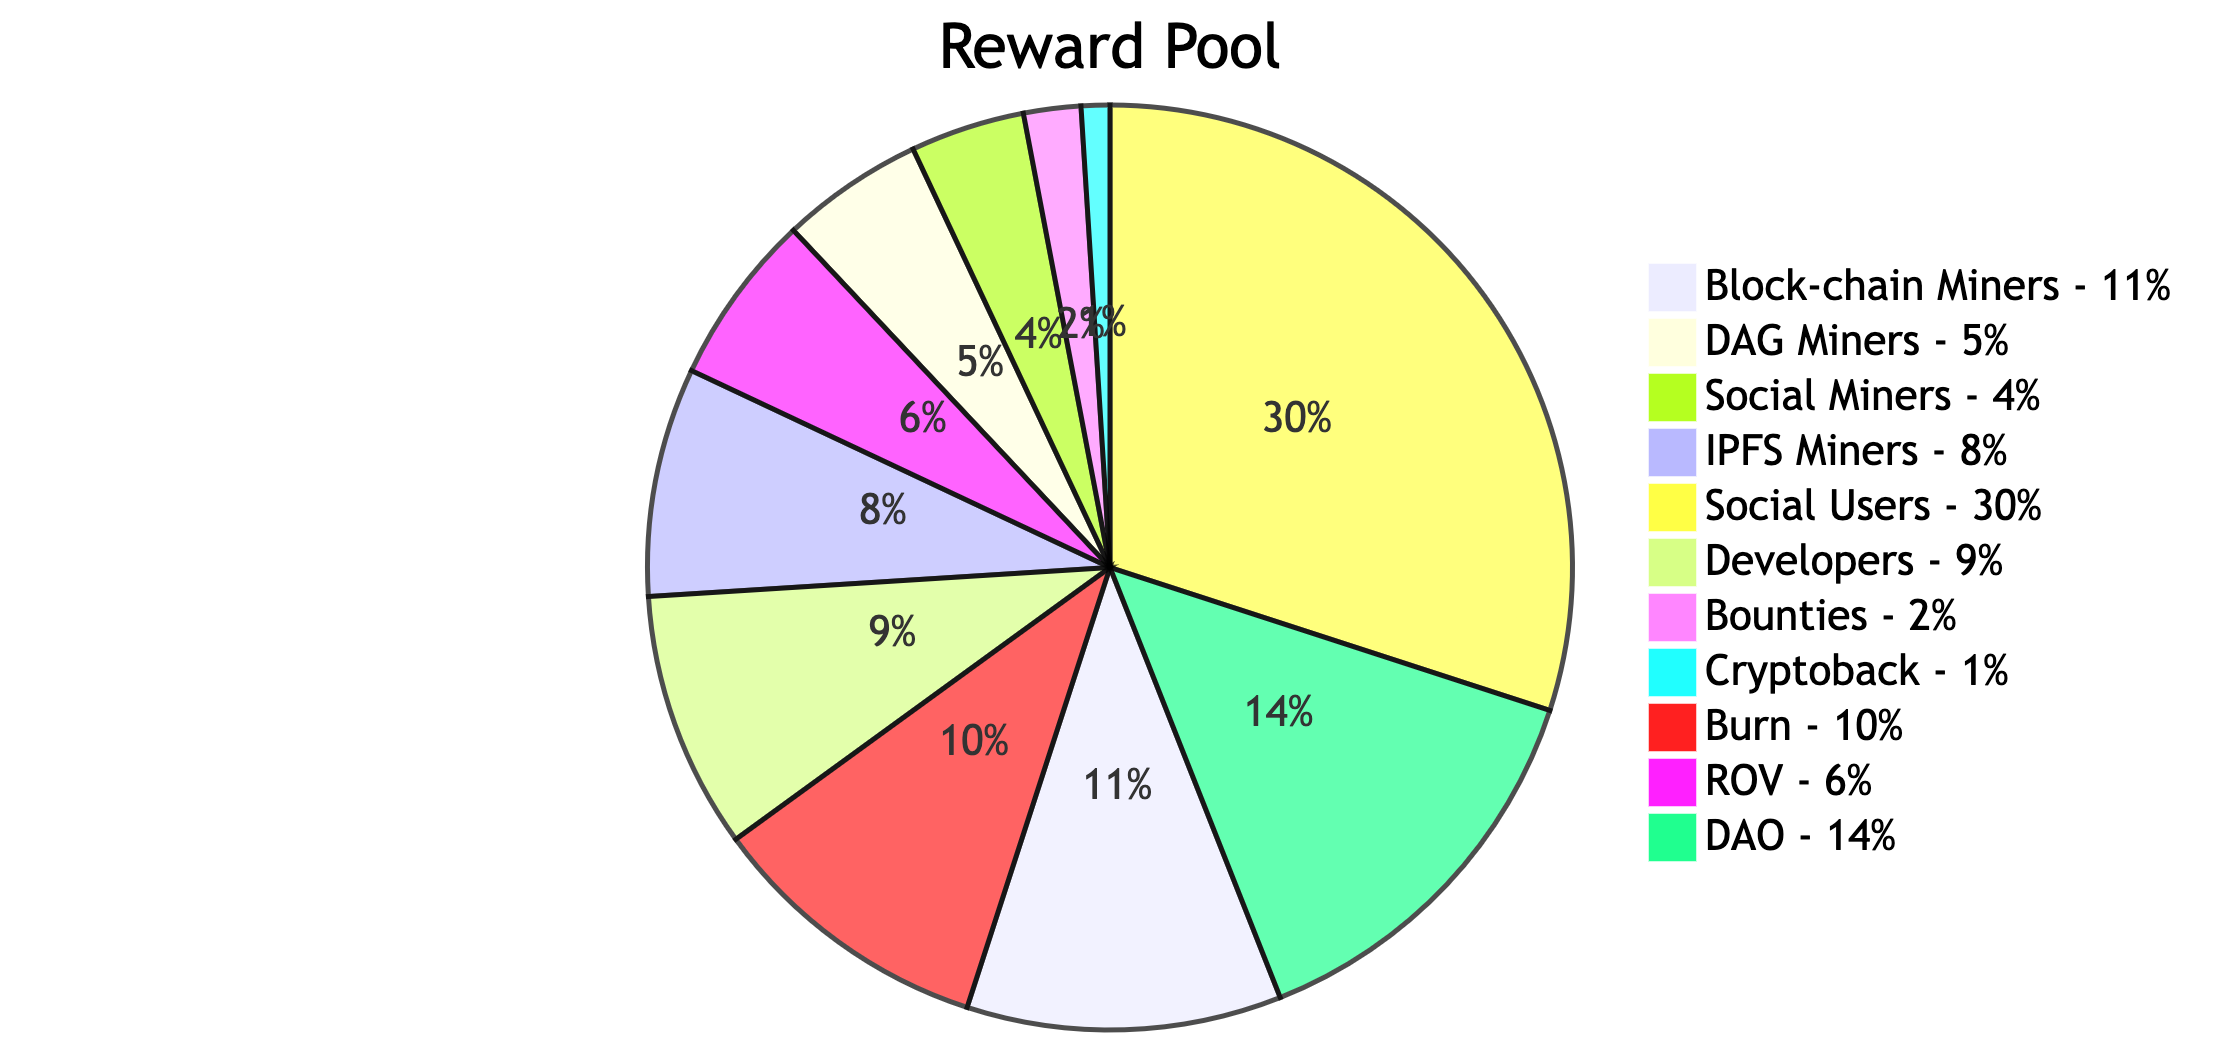
\includegraphics[width=8cm]{global-reward}
\caption{Allocation of Daily Revenue in percentage}
\end{center}
\end{figure}

\begin{enumerate}[wide, labelwidth=!, labelindent=0pt]
\item \textbf{Blockchain Miners} : For Viral Multi-Chain Validators according to total gas received per validator.
\item \textbf{DAG Miners} : For Tangle Full Nodes that stores \& mine transactions.
\item \textbf{Social Miners} : Nodes running relay servers of various decentralized tech-stack runs on Viral Social Application
\item \textbf{IPFS Miners} : Storage Viral IPFS Private Cluster nodes.
\item \textbf{Social Users} : For Social Application users according to their daily impression on their media content.
\item \textbf{Developers} : Allocated for Viral Open Source Developers allocated by amount of Shout-outs they receive for successful merge requests.
\item \textbf{Bounties} : Rewards for developers who can improve the applications by detecting major flaws and security loopholes.
\item \textbf{Crypto Back}: Similar to cash-back systems in payment applications. Viral Pay users will receive crypto-back for every payment they make.
\item \textbf{Burn} : Portion of the pool allocated to swap tokens to Viral Coin and sending it to a burn address where the supply will be removed.
\item \textbf{ROV} : Content Moderation community rewards according to their plus votes received for won polls.
\item \textbf{DAO} : Allocation for governing, maintenance and operation of the decentralized viral applications.
\end{enumerate} 

\begin{figure}[H]
\begin{center}
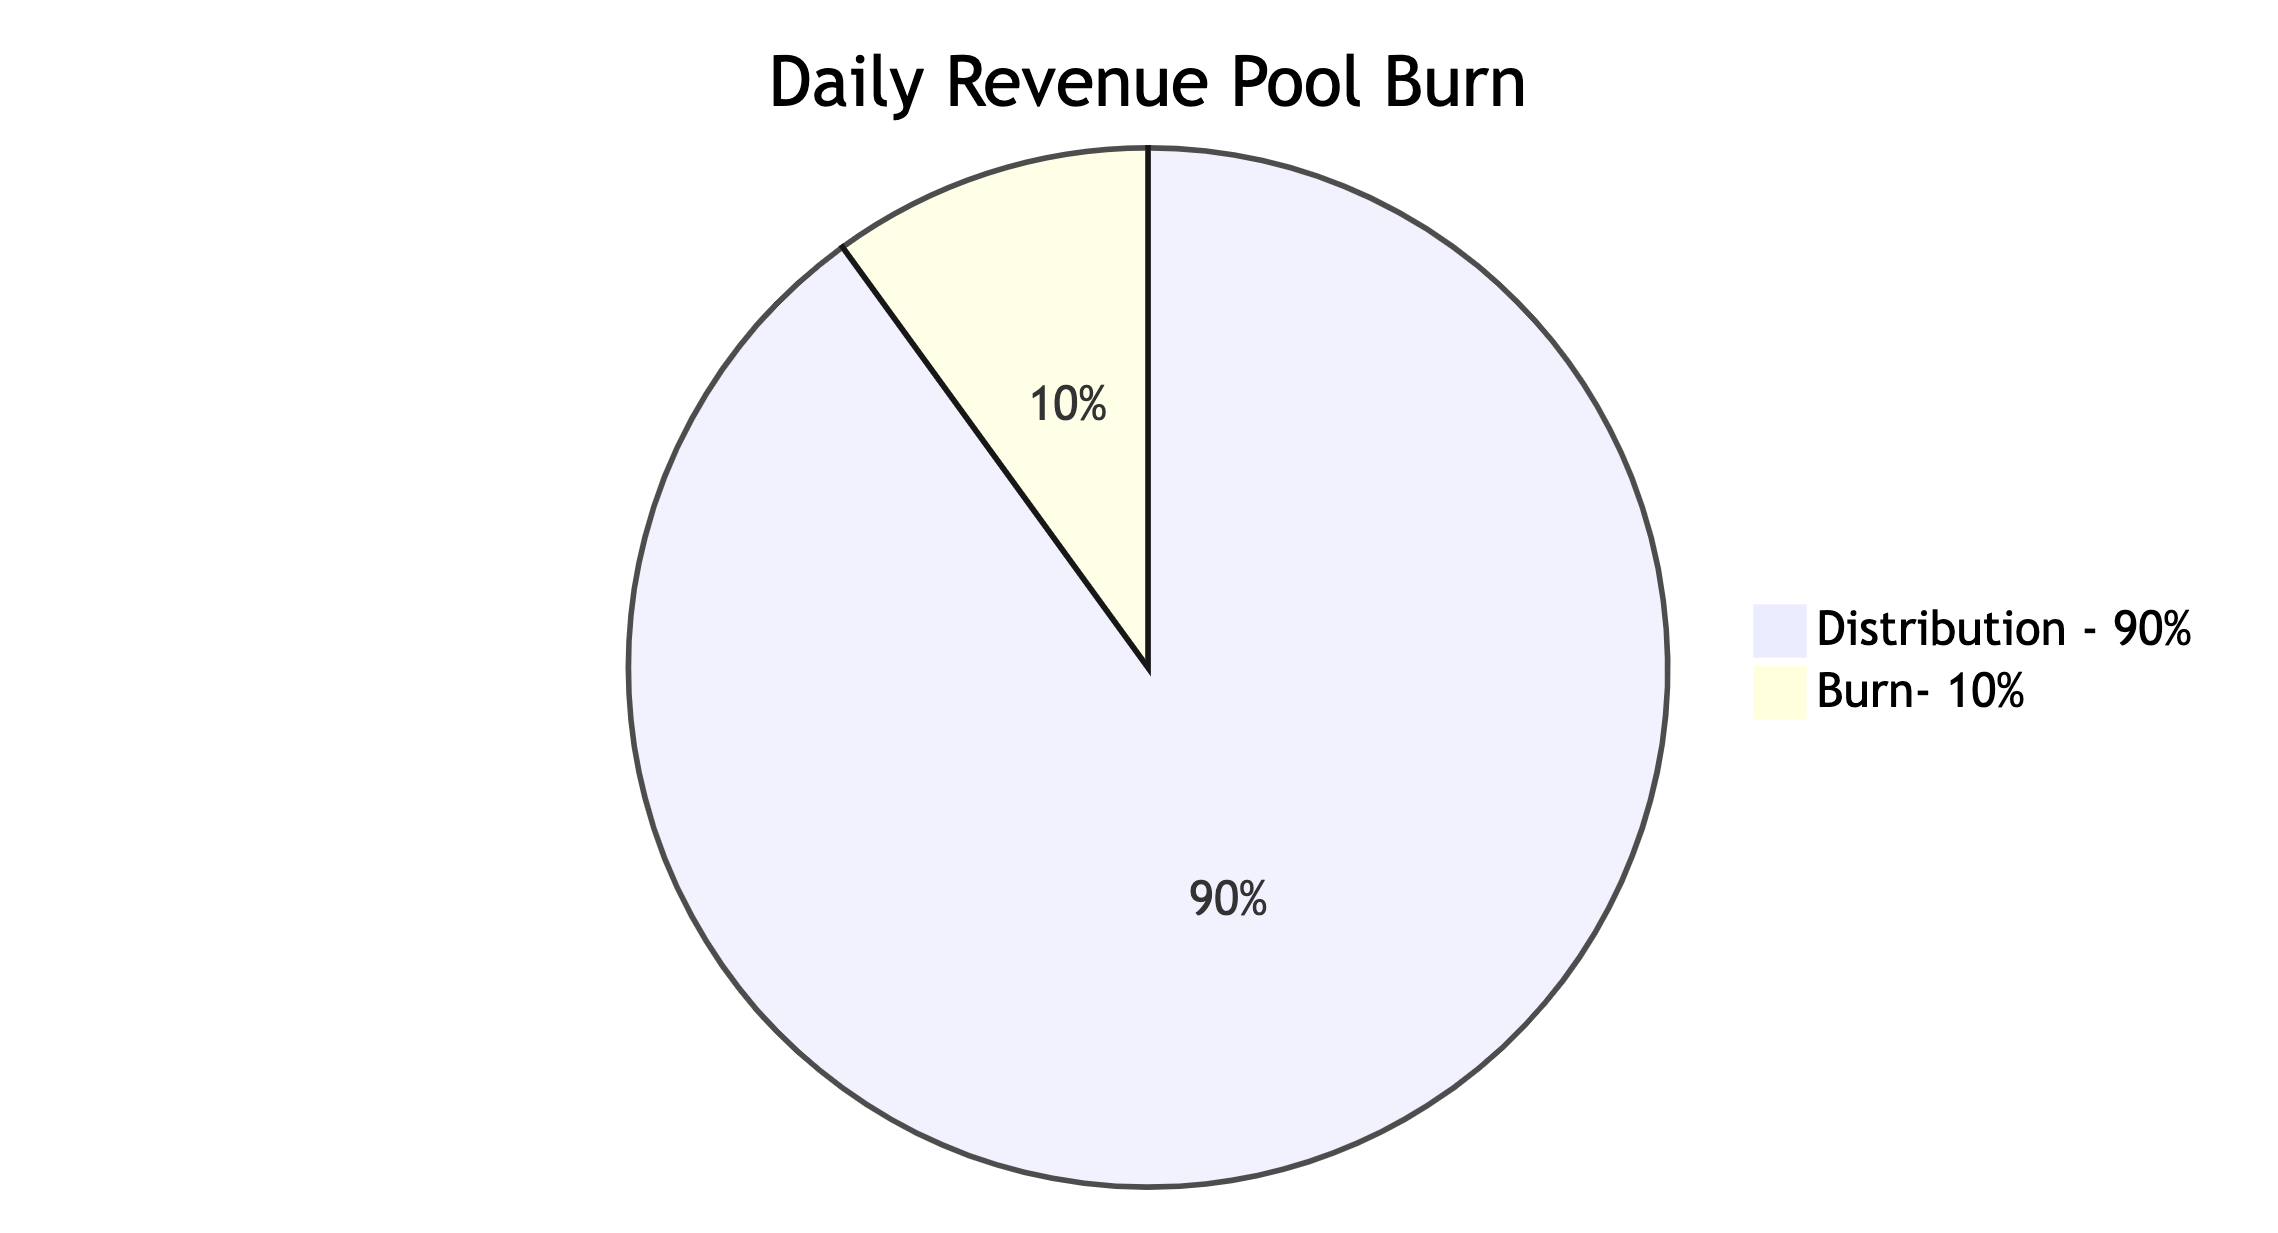
\includegraphics[width=8cm]{burn-chart}
\caption{Burn percentage from Global Reward Pool}
\end{center}
\end{figure}

\begin{figure}[H]
\begin{center}
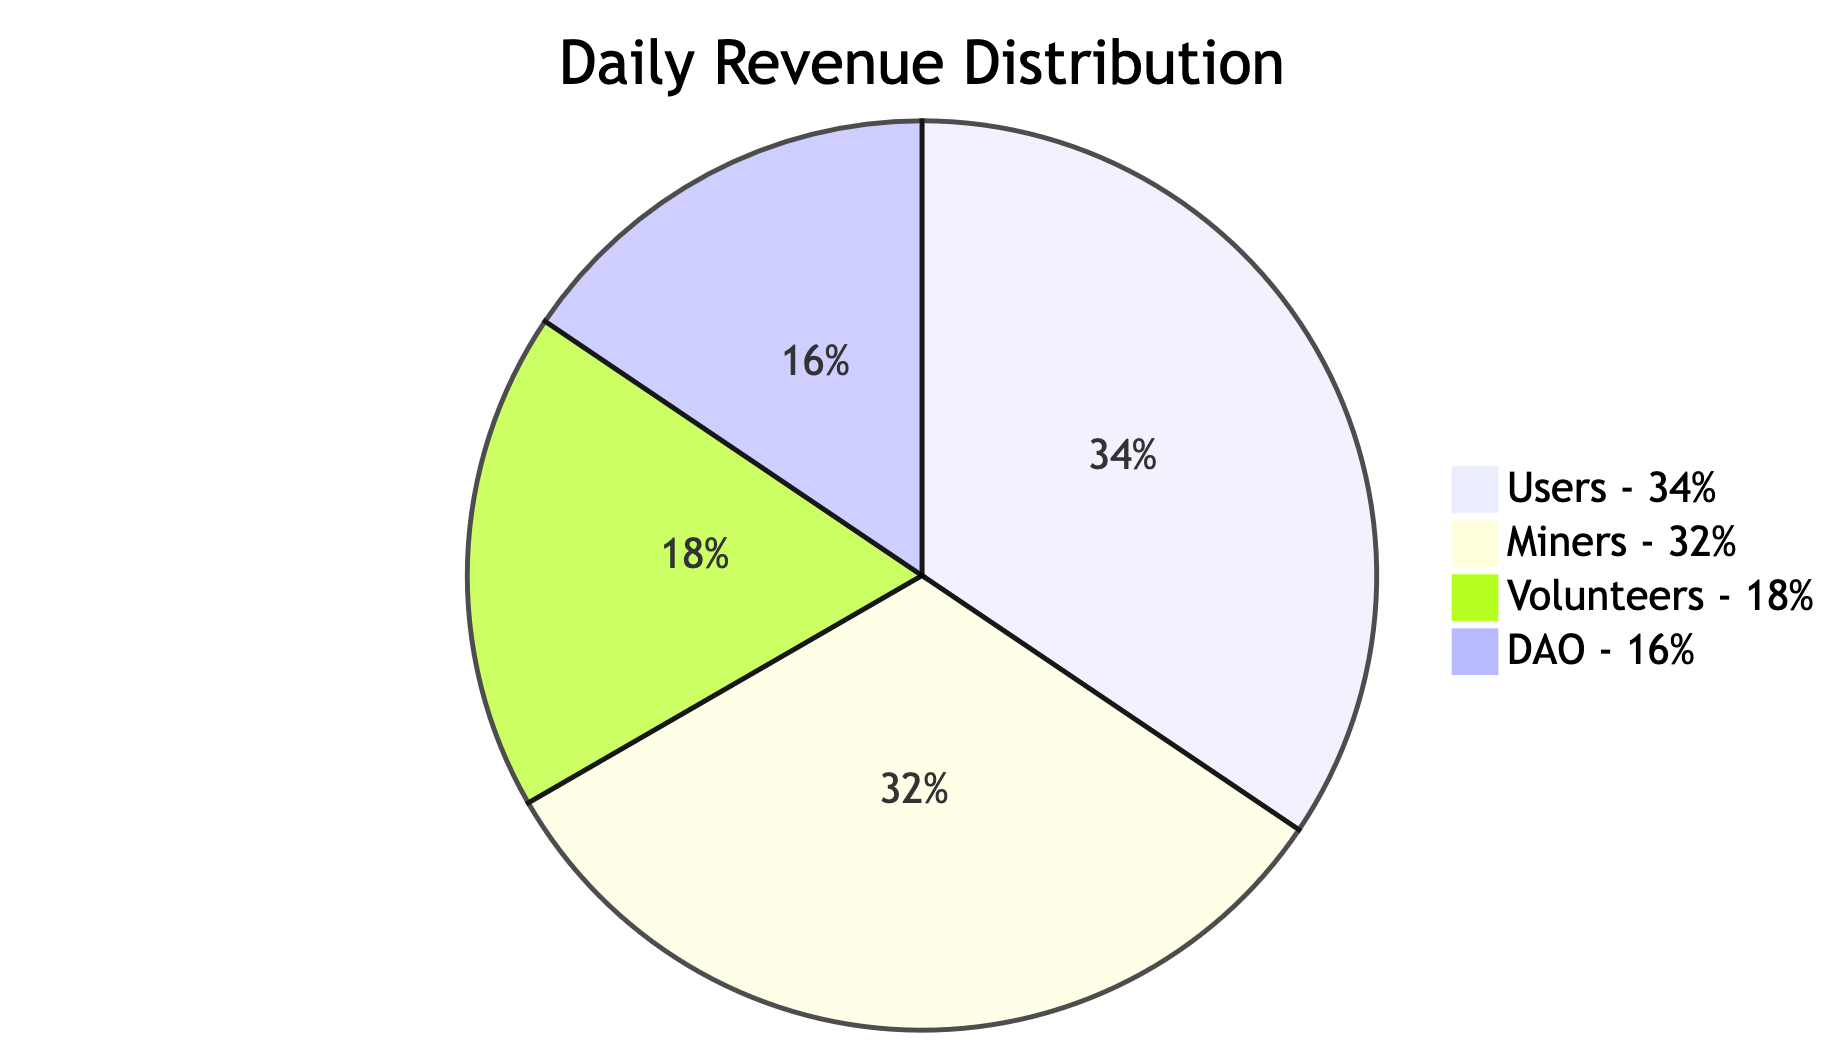
\includegraphics[width=8cm]{revenue-distribution}
\caption{Total Distribution of Funds excluding burn}
\end{center}
\end{figure}


\begin{comment}%mermaid

pie

    title Daily Revenue Distribution
    "Users - 34%" : 31
    "Miners - 31%" : 28
    "Volunteers - 19%" : 17.5
    "DAO - 15%" :  14

pie

    title Reward Pool
    "Block-chain Miners - 11% " : 11
    "DAG Miners - 5% " : 5
    "Social Miners - 4% " : 4
    "IPFS Miners - 8% " :  8
    "Social Users - 30% " : 30
    "Developers - 9% " : 9
    "Bounties - 2% " : 2
    "Cryptoback - 1%" : 1
    "Burn - 10% " : 10
    "ROV - 6% " : 6
    "DAO - 14% " : 14   
   
\end{comment}

\textbf{Portfolio of Multiple Tokens}\\

Viral rewards are multi-token rewards that are collected by various commissions across applications and services provided by the Viral DAO for the Viral Social Media and Viral Pay application. These rewards may include popular cryptocurrencies wrapped inside the viral smart chains such as Bitcoin, Ether, Solana, Cardano, Polygon MATIC, Binance USD, etc offered by the Viral Decentralized Bridge. Here, most of the tokens followed by Ether has 18 decimal places as it's smallest unit, each token has an ability to be transferred to one quintillion (one million trillion) accounts makes possibility of transferring a single token to over 4.66 billion internet users worldwide.  As nano-transactions creates huge amount of dust and bloats the size of the blockchain \& DAG ledger, the concept of Active Pool Percentage Allocation (APPA) is used to batch multi-token transfers and launch a manual method of air-dropping mechanism for the active-only users.  APPA takes a global and a local variable to calculate the percentage of rewards the global variable holds. In an example of user rewards which is determined by impression count, the global variable \textit{which holds the total reward tokens} represents the total impression and the local variable represents the number of impression received by the specific user which then calculates the percentage of rewards the local variable can acquire. The global and the local variable's data is received by the reward smart contract through decentralized oracles which  is made up of independent secure Sybil-resistant nodes for high availability and manipulation resistance. Thus promising security of off-chain data. \\

\begin{figure*}
\begin{center}
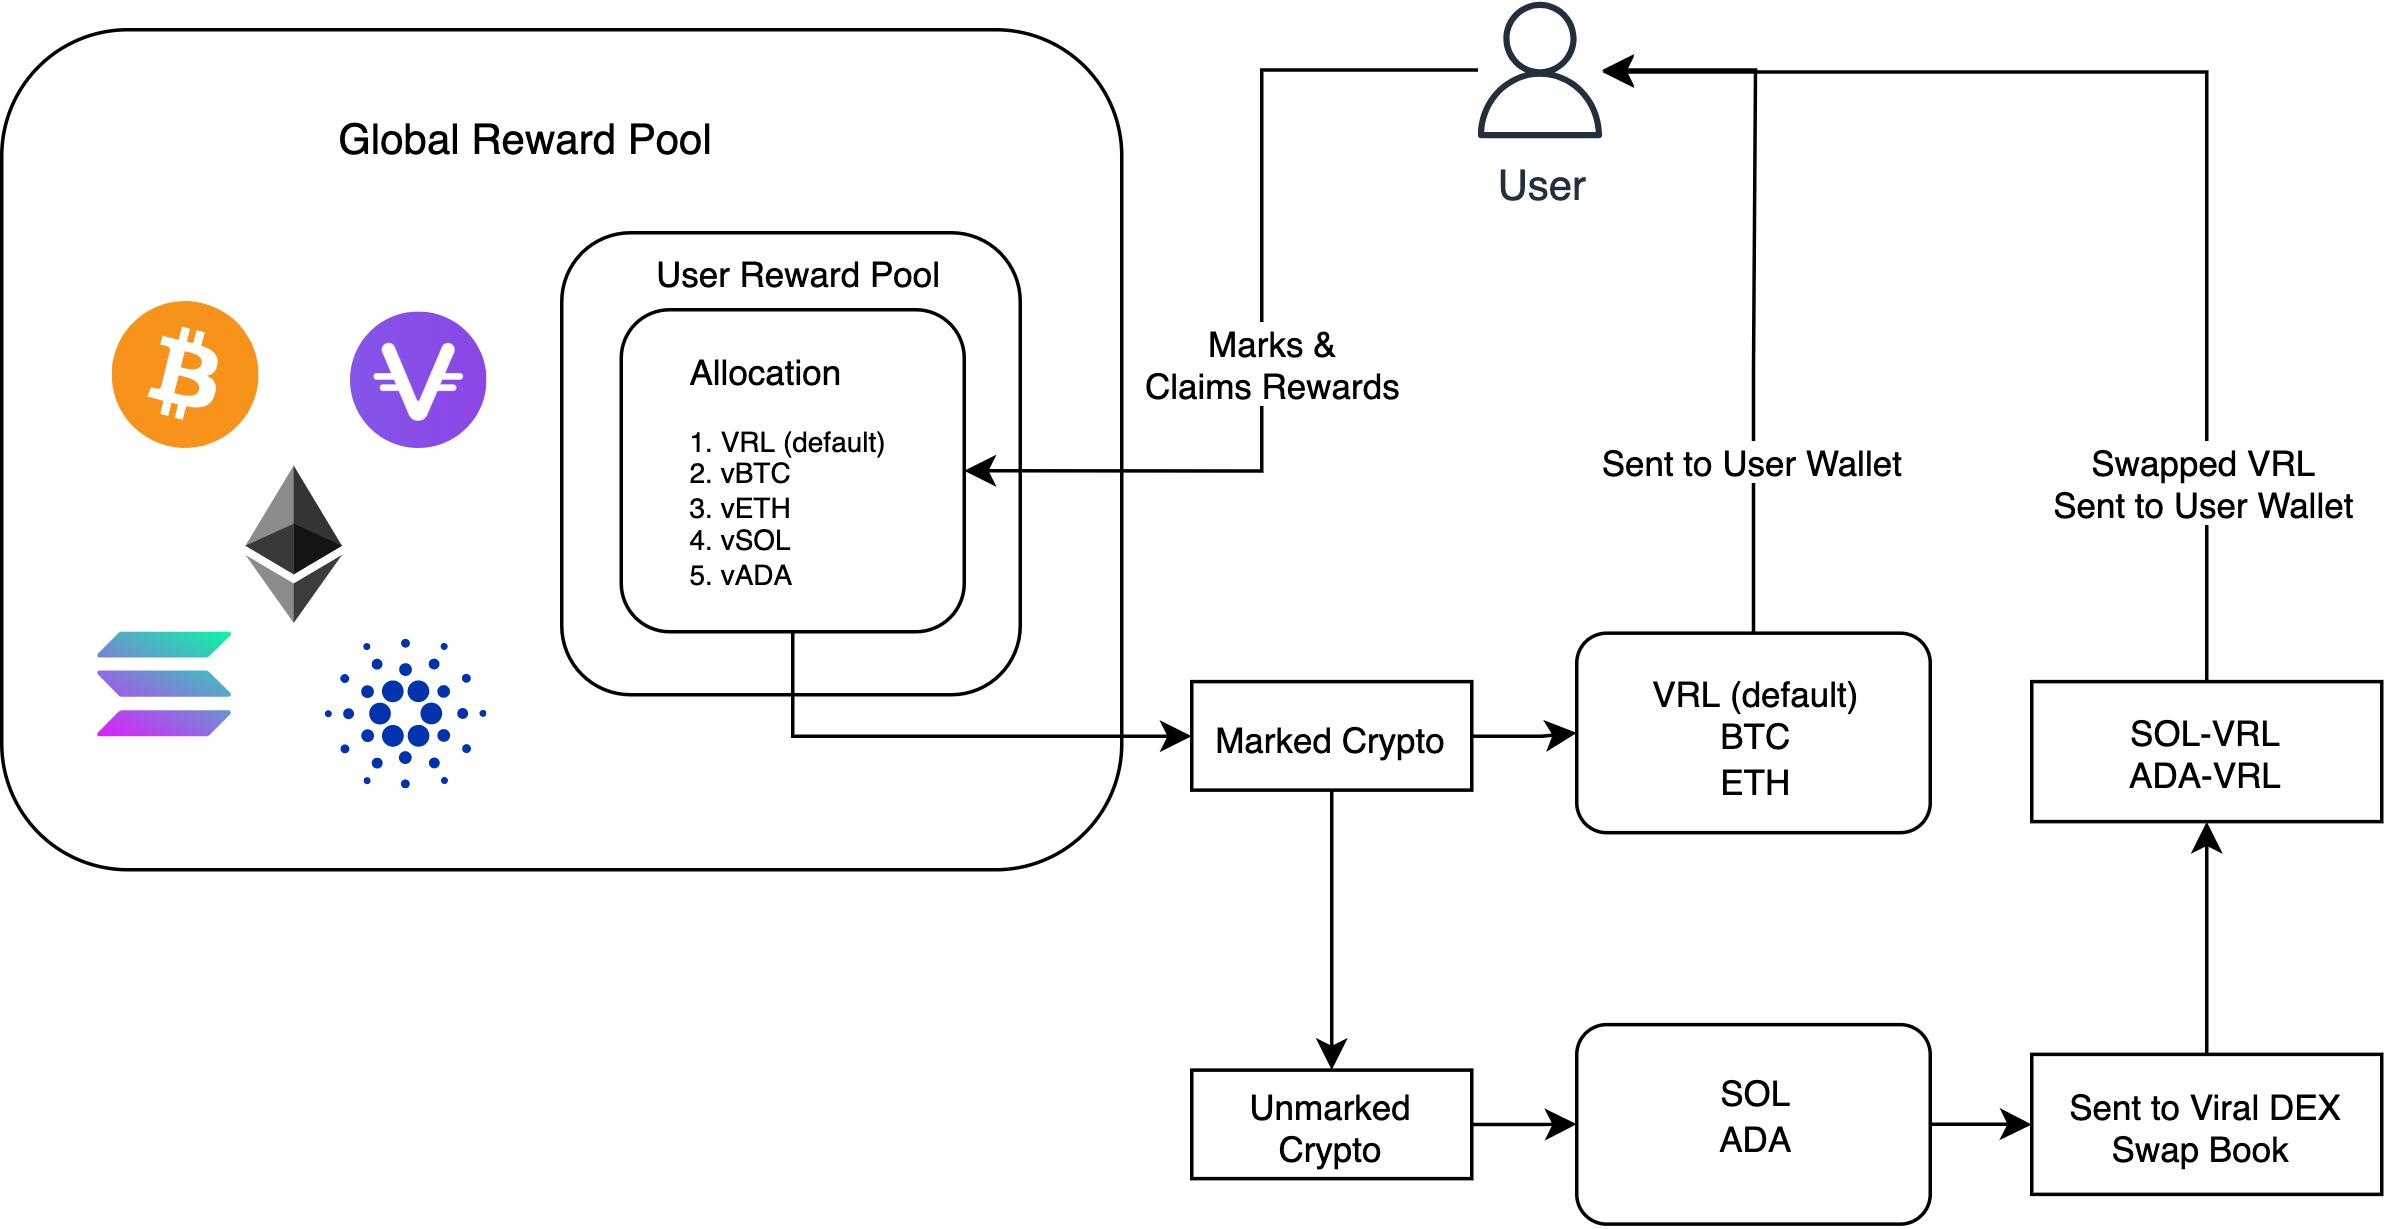
\includegraphics[width=12cm]{portfolio-reward}
\caption{Reward Allocation \& Claiming Multi-Tokens }
\end{center}
\end{figure*}

The reward allocation and claiming is done in simple steps,
\begin{itemize}[wide, labelwidth=!, labelindent=0pt]
\item The User's local variable and the Global variable is constantly fed to the decentralized oracles for a tamper proof record.  
\item After 2 AM UTC the rewards will be locked for the users to manually request \& receive from the pool. The user can choose the list of token's he/she is interested in i.e., Marked Tokens in which the default option of receiving VRL coins per reward allocation cannot be unmarked.
\item The user then calls the function in the specific reward pool smart contract e.g., user rewards, developer rewards, etc to withdraw his/her allocated awards.
\item The APPA is calculated by fetching the user's local variable and the platform's global variable. The percentage of funds is calculated and the withdrawal process is initiated.
\item The Marked tokens is directly deposited into the users wallet (VNS address/username), the unmarked tokens is then sent to series of (Unmarked Token - VRL) Viral DEX pools to swap for VRL tokens. 
\item The swap orders will be instantly added to the swap book and sent to users wallet once swapped successfully. For illiquid markets, the swap orders shall sit on the user swap book pending orders, which can be retrieved or cancelled at any time. This provides more liquidity to the DEX Pools.
\item The user successfully withdraws viral's multi-token rewards from a single transaction.
\end{itemize}

\textbf{APPA - Active Pool Percentage Allocation }\\

As mentioned above in the paragraphs, the viral rewards are allocated based on percentages of an individuals according to his/her contribution in the fully allocated rewards for all individuals eventually adding upto 100\%.  Viral Global reward pool maintains all the fees collected from users using various de-fi \& social applications, segregates and transfers the allocated percentages to various specific reward pools upon request by any-user after 2  AM UTC. Users, Miners, Volunteers are requested to receive their allocated rewards manually from the pools. The allocation per user is calculated by using the APPA algorithm which basically calculates the percentage of rewards by including a global and a local variable. The global variable is a sum of all existing local variable, typically total impressions, total shout-outs, etc\\
To explain the APPA algorithm which includes Local Percentage Calculation and Per-Token Reward Calculation an example of user rewards are taken into consideration.  The global variable $	\Psi$ represents the total impressions of all the users combined and the local variable $\lambda$ represents per-individual user's impression.  The Local Percentage is calculated as follows \\
\[Local\:Percentage(\lambda_p)=\frac{User\:Impression(\lambda)}{Global\:Impression(\Psi)} \times 100\]
The Per-Token Reward signifies the amount of tokens from a specific token $x$ is allocated for a specific individual from the pool. Since Viral incorporates multi-token rewards in which a single token having $x$ amount of units shall be distributed over all the pools for all the recipients of the reward. \\
\[Per-Token\:Reward(x)=\frac{Total(x) \times (\lambda_p)}{100}\]

\begin{figure}

\begin{lstlisting}[language=Solidity, caption={Example User Reward APPA Contract in Solidity}, numbers=none]


// SPDX-License-Identifier: MIT

pragma solidity ^0.8.4;

import "@openzeppelin/contracts@4.5.0/token/ERC20/ERC20.sol";
import "@openzeppelin/contracts@4.5.0/token/ERC20/extensions/ERC20Snapshot.sol";
import "@openzeppelin/contracts@4.5.0/access/Ownable.sol";
import "@openzeppelin/contracts@4.5.0/security/Pausable.sol";

contract Reward is Ownable, Pausable {
   
    uint256 public rewardamount;
    uint256 public rewardfortheuser;
    uint256 public impression = 0.0;
    uint256 public totalimp = 0;
    
    function pause() public onlyOwner {
        _pause();
    }
    
    function unpause() public onlyOwner {
        _unpause();
    }
    
    function totalrewardamount() external view onlyOwner returns(uint256){     // read 
         return rewardamount;
    }

    function finalimpression() external view onlyOwner returns(uint256){         //read
        return impression;
    }
    function finalrewardforuser() external view onlyOwner returns(uint256){      //read
        return rewardfortheuser;
    }

    function totalimpressionoftheday(uint256 totalImpressionOfTheDay) public onlyOwner{  //write
          totalimp = totalImpressionOfTheDay;
    }
    
    function claim(uint256 impressionoftheuser) public {                         //claim function
        require(totalimp != 0,"you cant claim your rewards yet");
        require(rewardamount != 0,"you cant claim your rewards yet");
        impression = ((impressionoftheuser*100) / totalimp);
        rewardfortheuser = (rewardamount * impression)/100 ;
        payable(msg.sender).transfer(rewardfortheuser);
    }

}
\end{lstlisting}
\end{figure}

\begin{figure*}
\begin{tcolorbox}

\begin{center}
\textbf{\underline{APPA Example in User Reward}}
\end{center}

User Impression ($\lambda$) = 10,000\\
Global Impression ($\Psi$)= 1,000,000,000\\
Total Reward ($x$) = 80,000 VRL, 500 BTC, 700 ETH, 1200 SOL \\

\[Local\:Percentage(\lambda_p)=\frac{10,000}{1,000,000,000} \times 100 = 0.001\%\]

\[Per-Token\:Reward(VRL)=\frac{80,000 \times 0.001}{100} = 0.8\:VRL\]
\[Per-Token\:Reward(BTC)=\frac{500 \times 0.001}{100} = 0.005\:BTC\]
\[Per-Token\:Reward(ETH)=\frac{700 \times 0.001}{100} = 0.007\:ETH\]
\[Per-Token\:Reward(SOL)=\frac{1200 \times 0.001}{100} = 0.012\:SOL\]

Output:\\
User Percentage of Rewards ($\lambda_p$) : 0.001\%\\
User Reward : \\
0.8 VRL \\
0.005 BTC \\
0.007 ETH \\
0.012 SOL\\
\end{tcolorbox}
\end{figure*}


\textbf{Reward Collection/Claiming Methods}\\

\begin{figure}[H]
\begin{center}

\begin{forest}
  forked edges,
  for tree={edge+={-Latex}},
  [Reward Collection
    [Restricted Periodic.C
    		[Users]
    ]
   [Dynamic Additive.C
   		[Volunteers]
    ]
   [Fixed Passive.C
   		[Miners]
    ]
  ]
\end{forest}
\caption{Reward Collection Types in Specific Pools}
\end{center}
\end{figure}

Rewards Collections are classified into three types - Restricted Periodic Claim,  Dynamic Additive Claim, Fixed Passive Claim. These different types offers claiming reward based on category of recipients and cause of rewarding. The reward collection methods will be hard-coded on the reward pools and cannot be updated with any DAO proposals, hence it is non-upgradable. Restricted Periodic Claim refers to offering rewards under a specific time period unless obtained cannot be withdrawn. The time period will be established according to the category of recipients a reward pool includes. If the rewards hasn't been claimed, the left-over cannot be claimed back and sent to a burn smart contract pool upon a claim request by any recipient after the time period. This ensures only active-participants to receive rewards with increasing the value of VRL tokens upon shrinking the token-supply by burning left-over tokens. The global variable is set at a constant number and will not be adjusted after withdrawals as the rewards are given for past-day's contribution. Restricted Periodic Claim is specifically used for larger recipient base with disproportionate contributions i.e., Social Users whereas Dynamic Additive Claim is used for active-volunteers with smaller base and consistent contribution towards the network i.e., Developers, ROV Curators. The Dynamic Additive Claim refers to offering rewards without a specified time where individual contributors allocations will be constantly adjusted/changed upon addition of new contributions recognized by the pool. The global variable is adjusted actively after every withdrawal and addition of local variable by recipients. This brings long-term reward pool holders to compete against each other for holding large portion of the pool while withdrawing and also short-term recipients desire to withdraw and cash-out quickly. The Dynamic Additive Claim doesn't includes a time period and the funds allocated for the recipients will be available openly for any-time to withdraw. Fixed Passive Claim is a straightforward claiming method for very-smaller number of recipients compared to Dynamic Additive Claim where the allocated rewards can be withdrawn any-time by the recipient by adding all the rewards allocated on each day which isn't withdrawn. Snapshots of allocated rewards will be updated everyday at 2AM UTC for the Fixed Passive Claim recipients to claim at once.\\

\begin{figure*}
\begin{center}
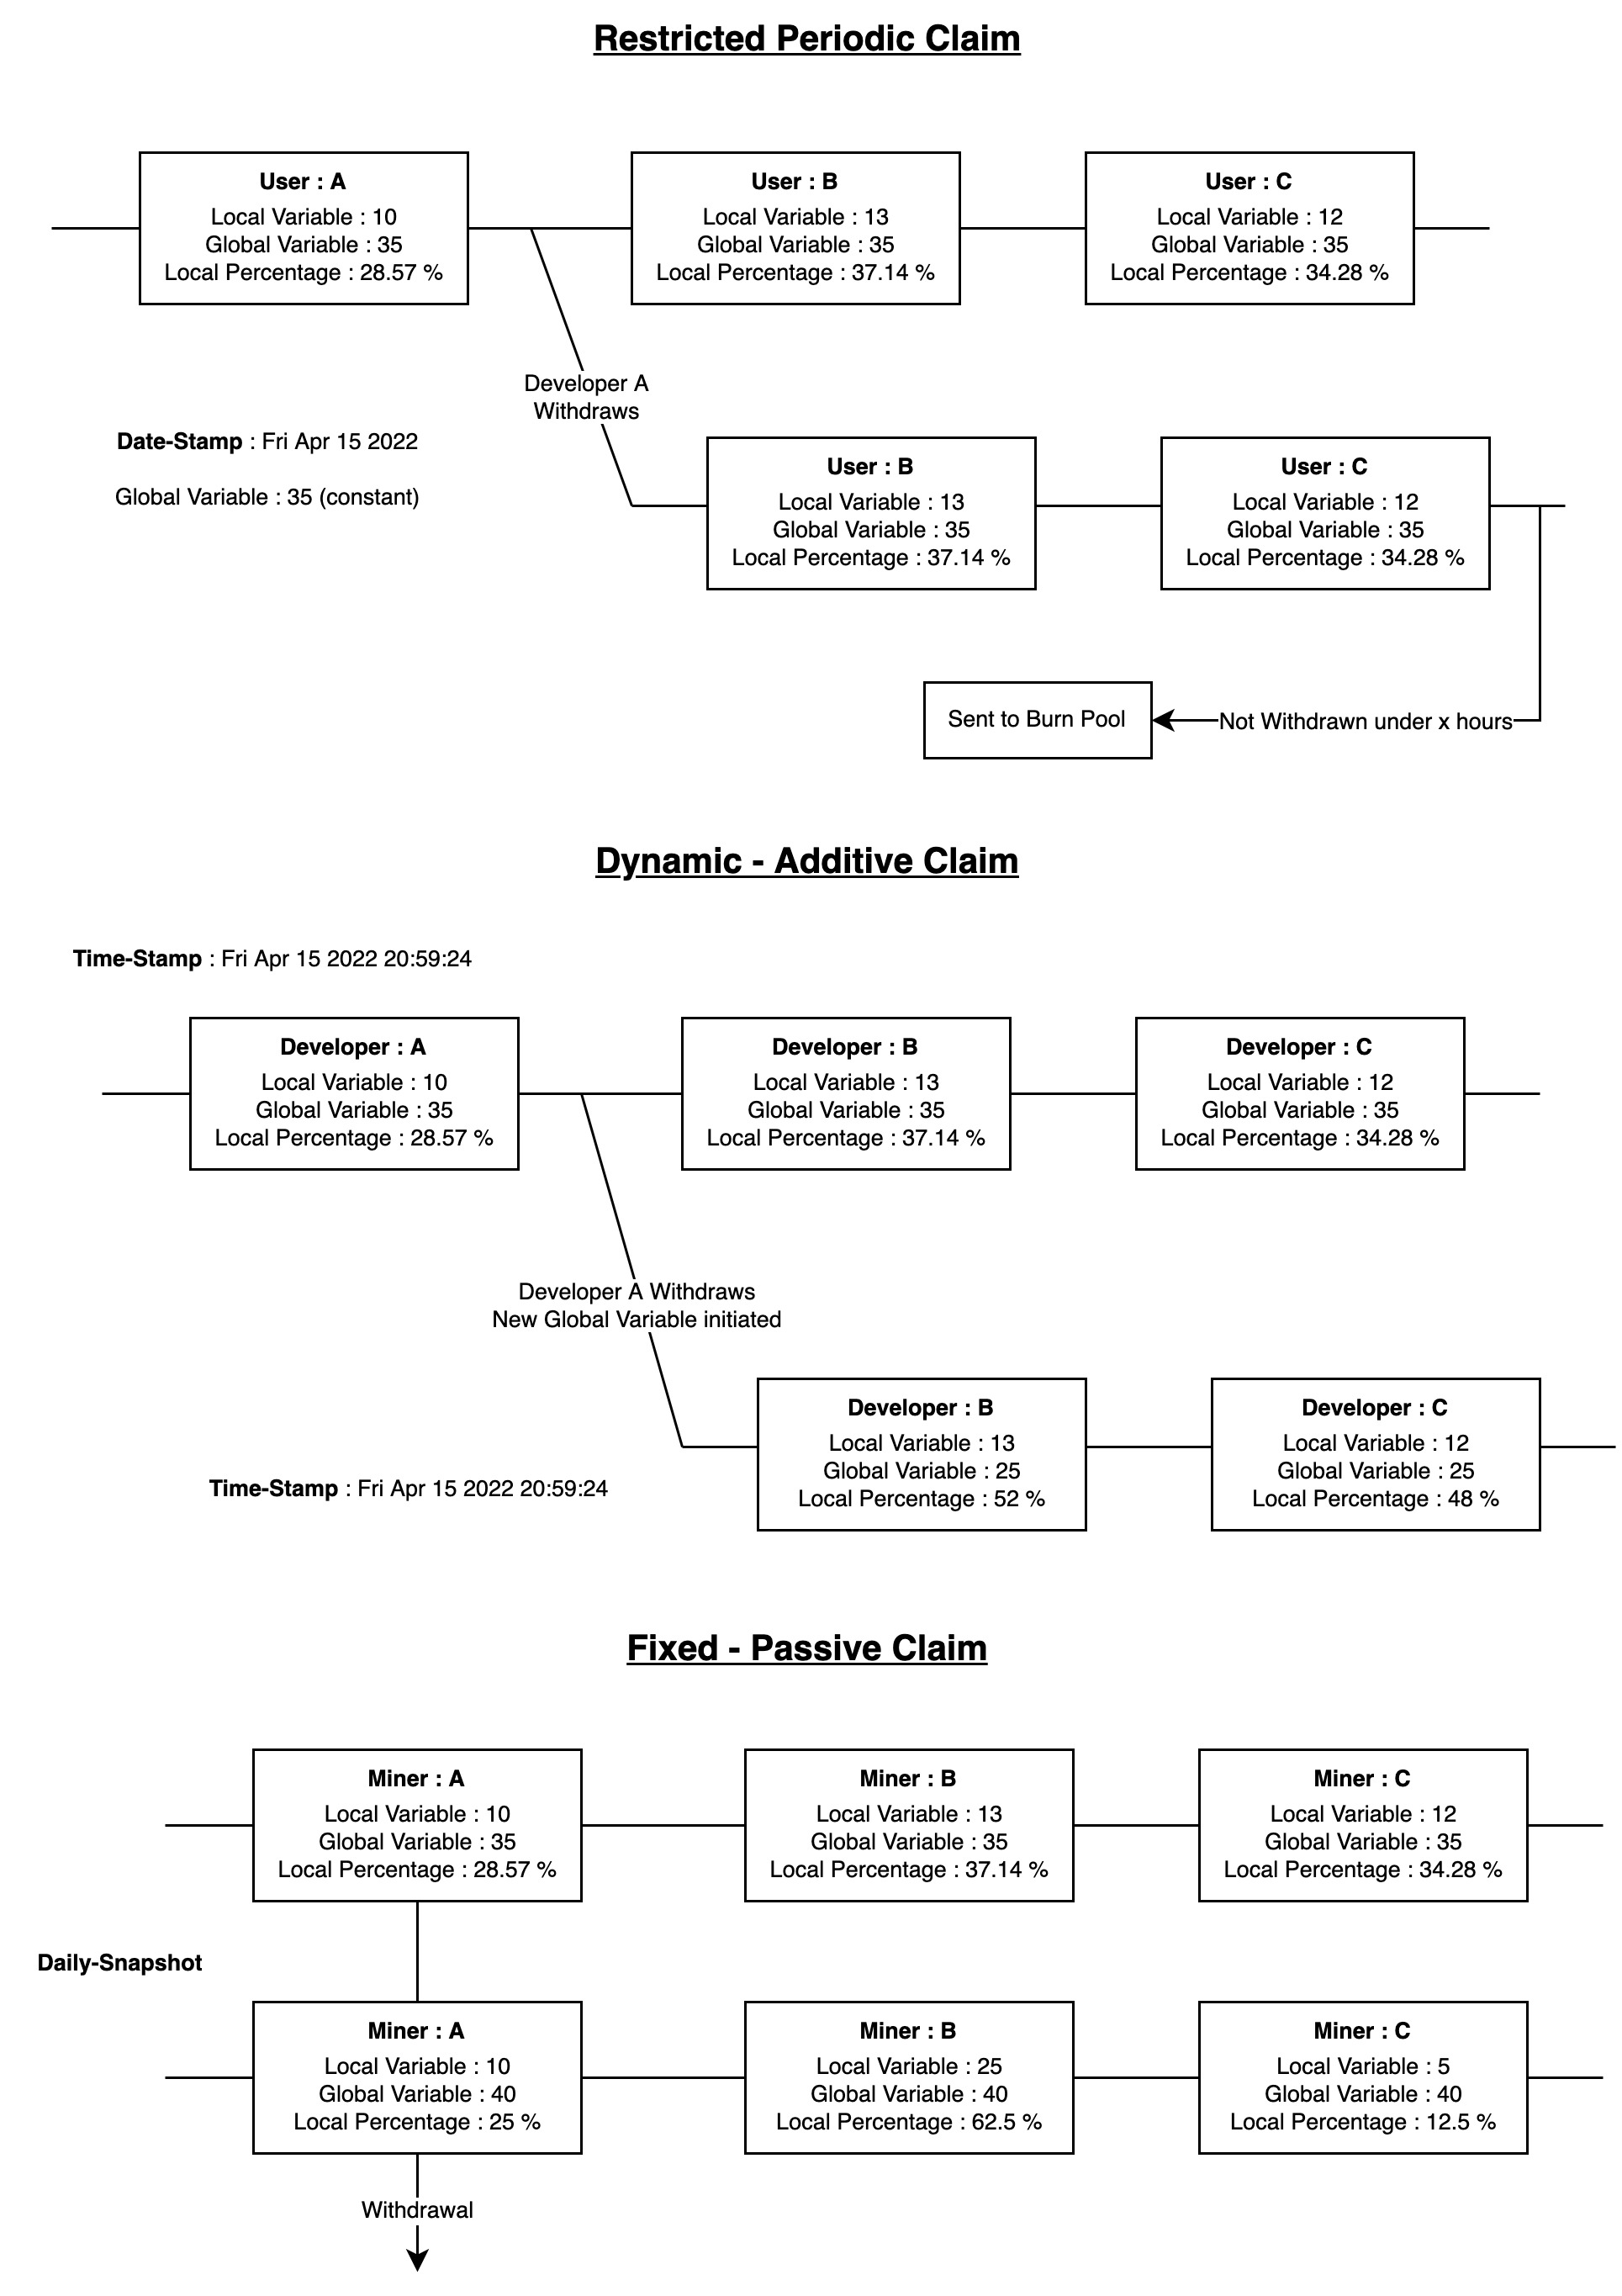
\includegraphics[width=15cm]{claim-rewards}
\caption{Differences between various Reward-Claiming methods}
\end{center}
\end{figure*}





\subsection{\textbf{Social Users (Impression-based) - 30\%}}

30\% of rewards from the global reward pool is allocated to Application Users based on the total views/impressions users get on their profiles. Impressions counts are agnostic to the type of content that is published in the Viral Application. Impressions/Views are a basic engagement of a typical post in all of social networking platforms. This ensures every content creator on the platform will get rewards according to their reach, popularity, and usage they get for their content on the decentralized platform. This can keep content creators getting paid every day according to the traffic they receive on their profile/content they post. The rewards are allocated to the user reward pool from the global reward pool every day at 2.00 AM UTC. The Restricted Periodic Claim is set to 14 hours for manual collection. The users can mark their preferable tokens while the unmarked tokens will be sent for swapping to the Viral DEX swap order book. The pending swap orders will be exchanged for VRL token and will be dropped directly to the user's VNS address/username. After the 14 hour window the funds in the unclaimed tokens in the user-reward pool will be transferred to the burn pool and cannot be claimed back.\\

\begin{center}
\textbf{Global Variable} $\to$ Combined Impressions of all users / day\\
\vspace{2mm}
\textbf{Local Variable} $\to$ Total User Impression / day\\
\vspace{2mm}
\textbf{Claiming Method} $\to$ Restricted Periodic Claim = 14 hours\\
\end{center}

\textbf{Advantages}
\begin{itemize}[wide, labelwidth=!, labelindent=0pt]
\item Creators can be able to create content expecting a reward for it
\item A fair share of rewards according to the popularity of the content.
\item Users will trust the platform which gives them 30\% of it’s daily collected revenue to every user without any centralized company meddling.
\item Encourages other platform users to join and receive multi-token rewards.
\end{itemize}

\subsection{\textbf{DAO - 14\%}}


\subsection{\textbf{Blockchain-Miners (Gas-based) - 11\%}}

Written After Blockchain\\

\subsection{\textbf{Burn - 10\%}}
\begin{figure}[H]
\begin{center}
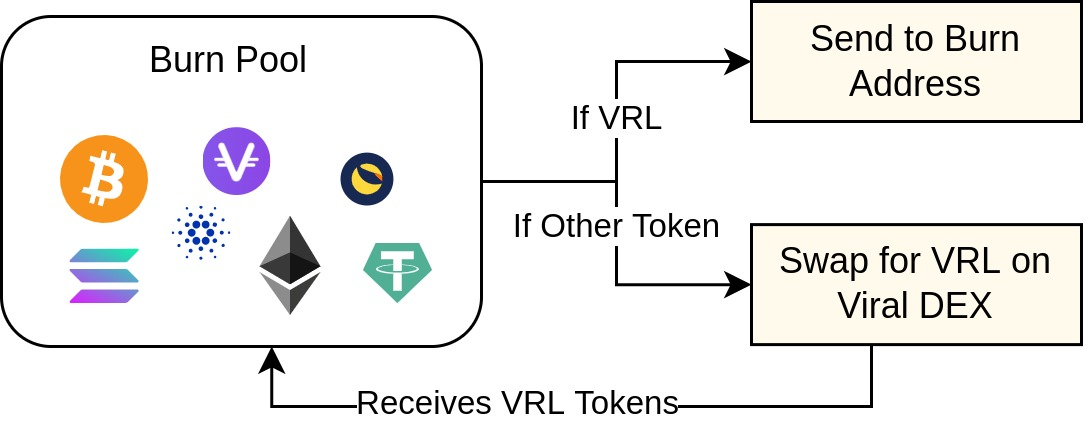
\includegraphics[width=7cm]{burnpool}
\end{center}
\end{figure}

Burning tokens represents permanently removing $x$ amount of tokens from the circulating supply. This process of burning tokens is carried out by transferring the tokens to a burn address i.e., a wallet address which do not have a private key which means the tokens are gone forever. This method is often described as destroying tokens.  Burning VRL (Viral Coin) tokens are used for deflationary purposes by decreasing the supply driving the token's price upward where the traders and investors gets incentived. As VRL token is the default reward token and the utility token of the Viral Social Media and the blockchain applications, the coin's automated deflationary mechanism through the reward pool allocating 10\% of it will incentivize the holders, reward recipients, etc by adding scarce in availability and more value to existing tokens. Since the burn pool may consist of many different tokens, they'll be sent to Viral DEX swap book's for swapping all the other tokens to VRL Tokens, later sent and burnt accordingly.This burned tokens include 10\% of all kinds of fees involved in the blockchain, social and de-fi applications.\\

\subsection{\textbf{Developers (Contribution-based) - 9\%}}

9\% of rewards from the global reward pool is allocated to Developers. Viral is an Open-source platform where developers contribute to available viral open source repositories and get rewarded for their contribution to the decentralized platform and also to encourage developers by making awareness about the POSI - Paid Open Source Initiative to structure a better, safer, secure social media for the masses using collaborative work is the ultimate goal. By bringing mass development to life we can ensure that the people who run social media will be the product of hundreds of developers working every day for a common goal of a powerful social communication platform. We will be linking developers' GitHub and viral accounts in a separate ROV-Dev Application in which the developers can contribute their work and get shout-outs by other developers for rewards. The shout-outs will determine their rewards where the largest receiver will be allocated with more tokens.\\ 

Every single developer should be rewarded fairly for their work and the rewards should be determined by their fellow developers inside the community. Since there is no meddling of Viral DAO and its executives, the developer platform will be democratic, decentralized, and autonomous to keep the social media strong and secure in the most possible way. By rewarding developers, we can expect other developers to join the people-run social media.Viral will give a better world to developers expecting a reward for their contribution and also engages a lot of developers into a small community to get most of the percentage from the allocated 9\% of daily revenue to a closed community. This will encourage autonomous development of superior technology where all hands matter. \\


\begin{center}
\textbf{Global Variable} $\to$ Combined Shout-Outs of all developers\\
\vspace{2mm}
\textbf{Local Variable} $\to$ Total User Shout-Outs\\
\vspace{2mm}
\textbf{Claiming Method} $\to$ Dynamic Additive Claim\\
\end{center}

In Dynamic Additive Claim the Global variable get's constantly updated adding up the total local variables, compared to the Restricted Periodic Claim's constant global variable specified per day.  The allocation of reward gets updated after every withdrawal and addition of various merge-request contributions. \\


\subsection{\textbf{IPFS-Miners (Storage-based) - 8\%}}

After IPFS\\

\subsection{\textbf{ROV (Contribution-based) - 6\%}}

6\% of rewards from the global reward pool is allocated to ROV (Republic of Viral), a content moderation community for the Viral Decentralized platform. There, curators will be filtering and voting posts to eliminate spam, inappropriate content which is reported by users and also govern the application's content in a democratic nature considering every curator's vote. This method of democratic voting community eliminates the power of a single individual to decide the type of content if it's violating the social media's posting guidelines. This ensures rapid results in removing explicit content in a relatively short time without any hassles. In short, ROV is a decentralized autonomous organization to maintain Viral's media contents at its best. The curators will be rewarded by Viral Coins for their contribution to the network.\\

\begin{center}
\textbf{Global Variable} $\to$ Combined Positive Points of all Curators\\
\vspace{2mm}
\textbf{Local Variable} $\to$ Total Positive Points\\
\vspace{2mm}
\textbf{Claiming Method} $\to$ Dynamic Additive Claim\\
\end{center}

\textbf{Advantages of ROV over Centralized Organization}
\begin{itemize}[wide, labelwidth=!, labelindent=0pt]
\item Faster content removals
\item The decision of a single organization/person will be eliminated
\item A better-decentralized approach to centralized organizations
\item Will work in any time zone 24/7 without any hassles
\end{itemize}

The transfer of funds from global reward pool to the ROV Pool will be carried at 2 AM UTC where the curator's Plus points for the day will be taken and the percentage of rewards will be determined using it. The ROV Pool uses the  Dynamic Additive Claim algorithm in which for every positive contribution the curators make the points will be increased and the local percentage will be adjusted in allocation of rewards. Every curator shall be able to withdraw their reward any-time they would want to.\\

\subsection{\textbf{Social Miners (Serving based) - 4\%}}

Social Miners are people running nodes in the viral decentralized network for storing media and data transfers. It is similar to blockchain mining nodes but here the nodes will run Gun DB Relay server, WebRTC signaling server, and other several mini peers of other stacks simultaneously to provide faster data transfer, decentralization of data, higher encryption, better stability, etc. Users can download the node software and run the program to become a social node for the Viral network and start earning rewards according to the data served for the network\\

Others after\\

\subsection{\textbf{DAG-Miners (Transaction-based) - 5\%}}

After DAG Tangle\\

\subsection{\textbf{Bounties - 2\%}}

Viral runs a daily bug bounty program called the Viral Find Vulnerability Program (VFVP) is an intiative which rewards ethical hackers and penetration experts to discover software bugs which possesses a threat to the software's security. Viral rewards individuals who report the bugs through the dev-space platform and receive shout-outs from the developers from specific projects. The specially allocated 2\% is only to reward bounties and uses the Fixed-Passive Claim algorithm for claiming the rewards. \\

\subsection{\textbf{Crypto-Back - 1\%}}

\subsection{\textbf{Charity Contribution}}

If the user opts for transferring the rewards to a Non-Profit-Organizations it can be easily transferred directly to the user's preferred Charity. Viral will have a registration portal for Charities to Register their information and get verified to appear on the Application's Wallet.\\ 



\section{\textbf{Governance \& Viral DAO}}

Viral incorporates a vast ecosystem of blockchains and De-Fi application along with the integration of social networking for the masses to adopt cryptocurrencies to the fullest. While aiming for a true-decentralized product, governance plays a huge role in every aspect of decisions on updating the protocols. Most de-fi organizations have separate on-chain governance communities apart from offline-governance to vote and improve their platforms, Viral prepared to seperate governance of current and future products into two governance models and bring decentralized decision making oppurtunity for the members of the community. The Viral Foundatoin decided not to bring in any centralized governance model for any of it's ecosystem except the ViralFEX since it complies with regulatory restrictions.\\

\textbf{Governance Models}\\

\begin{figure}[H]
\begin{center}

\begin{forest}
  forked edges,
  for tree={edge+={-Latex}},
  [Governance
    [Smart Chain Governance
    ]
   [Ecosystem Governance
    ]
  ]
\end{forest}
\caption{Governance Model}
\end{center}
\end{figure}

While governing Viral Smart Chains protocols requires validators and nodes on voting consensus, the mobile application comprising de-fi protocols requires a decentralized autonomous organization (DAO) to vote on frequent updates and maintenance of offline compliances. This model for governance is seperated among validators (miners) and DAO Token Holders.\\


\textbf{Viral Smart Chain}\\

On-Chain Governance\\
Staked Tokens\\
Viral Improvement Proposal\\
Addition of New Chains\\

\textbf{Viral Ecosystem Governance}\\

DAO \& Intro to Decentralized Governance\\
Centralized companies vs decentralized organizations\\
How expenditure, revenue, profits and other basic financial terms in companies work in a decentralized environment\\
Popular DAOs History, debates, failures and lessons to be learnt\\
Viral DAO Intro\\
Viral Foundation and V-DAO\\
What type of Governance V-DAO Do?\\
Tokenization of Rights - Intro\\
List of Tokens and its significance\\
Staking and Unstaking of tokens\\
Detailed Explanation of each token, ratios, holding benefits, etc\\
V-DAO Platform Introduction\\
V-DAO Proposals Intro\\
V-DAO Proposals - Detailed Explanation\\
V-DAO Treasury Types and how it can be withdrawn, etc\\
Distribution of Profits as Dividends\\
Dividend Detailed Information\\
Monthly Operations Proposal - Its Significance and How it will be passed monthly\\
Reward Pool Alteration Proposal - Every 4 months\\
No-Dividend Proposal for Higher Cost Development work\\
Rights of Holders\\
Initial Sale of V-DAO Tokens for Viral Coins\\
Minting Procedure of Each Tokens for Further Treasury Funding\\
Emergency Procedures in case of any event\\
Centralized Entity Affiliations for Operations through only Viral Foundation\\
Decentralized Entity Affiliation  and contribution to Reward Pool\\
Delegating of Voting Rights to certain cabinet holders\\


\section{\textbf{Tokenomics \& ICO}}

\begin{enumerate}[wide, labelwidth=!, labelindent=0pt]
\item \textbf{Name of the Utility-Token} : Viral Coin
\item \textbf{Ticker of the Token} : VRL
\item \textbf{Pre-mined Tokens} : 5,000,000,000 Tokens will be issued 
\item \textbf{Supply Hard-Cap} : 5,000,000,000 Tokens
\item \textbf{Token Nature} : Deflationary
\end{enumerate}

\begin{figure}[H]
\begin{center}

\includegraphics[width=2.5cm]{viral-coin-logo}
\caption{Viral Coin Logo}
\end{center}
\end{figure}

\begin{figure}[H]
\begin{center}
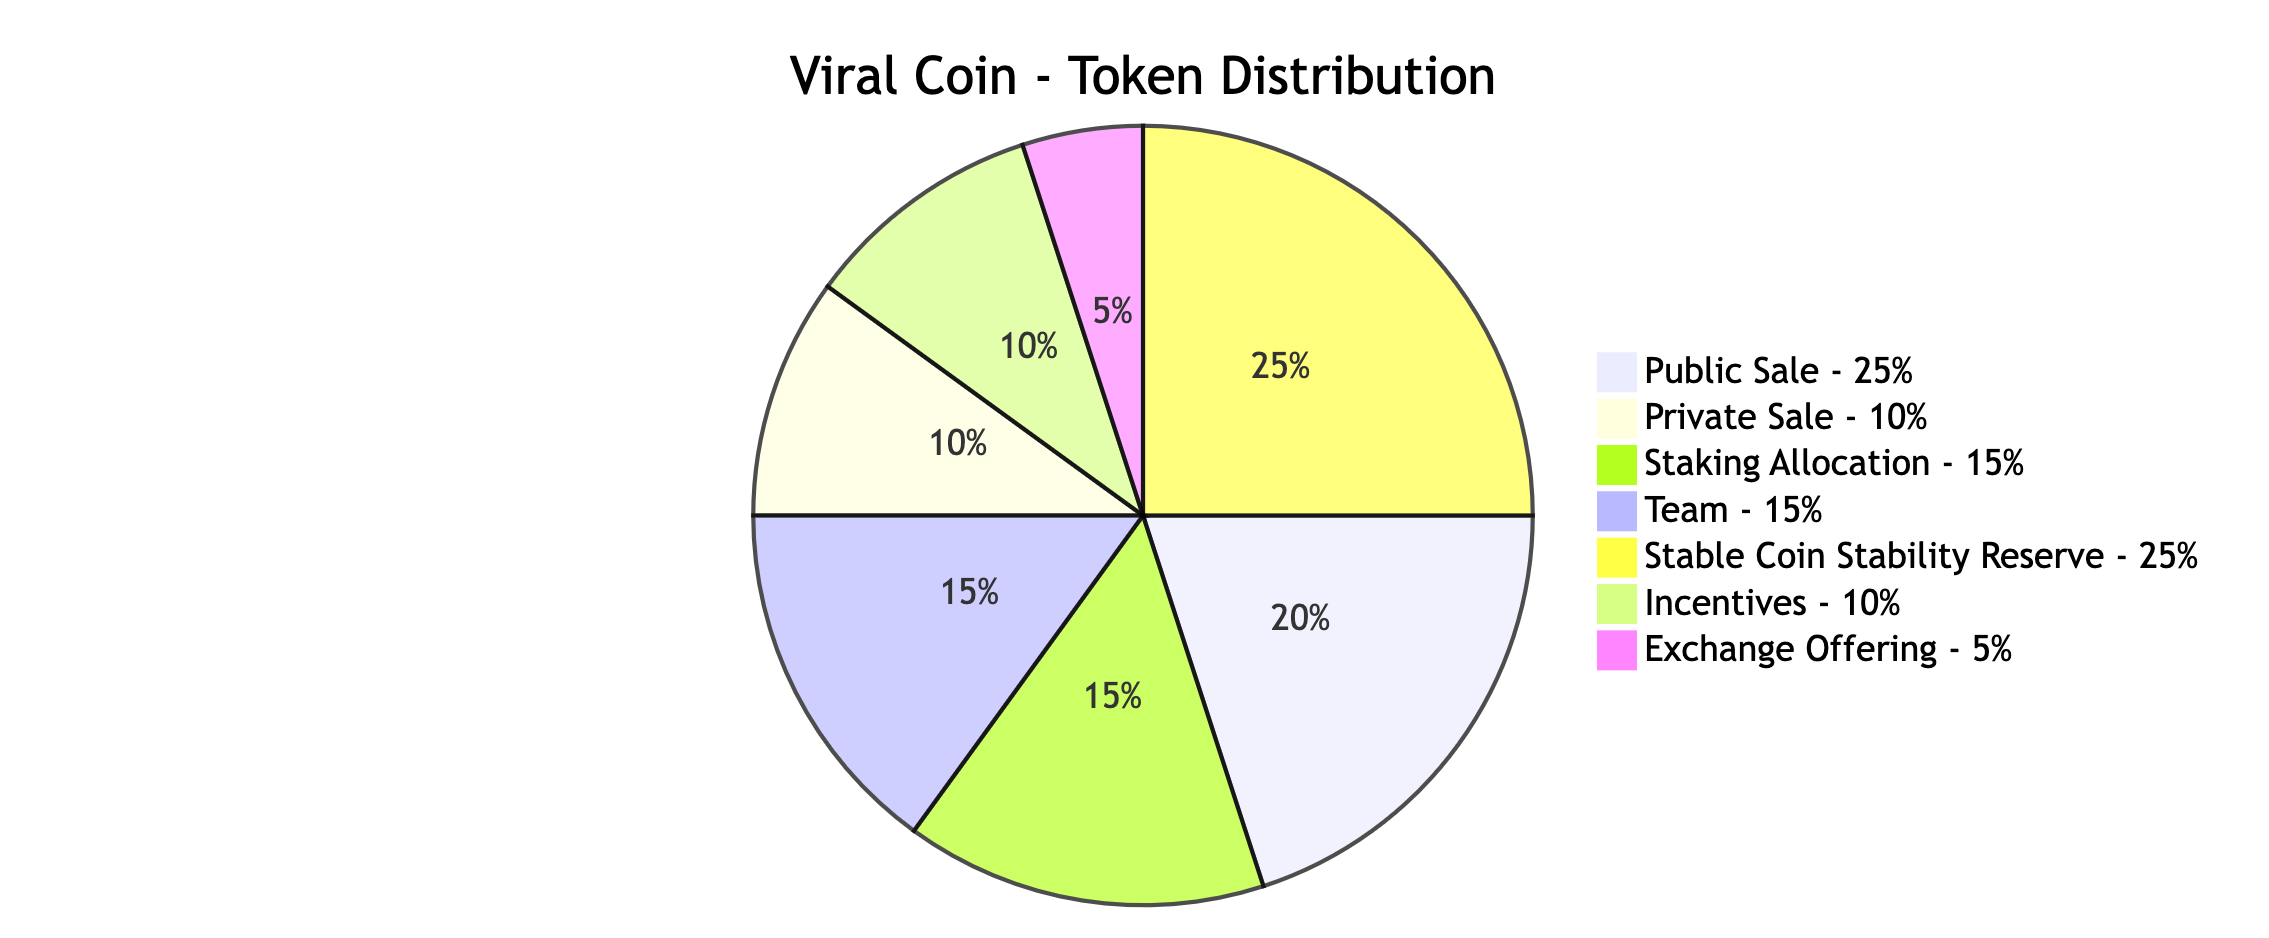
\includegraphics[width=10cm]{token-distribution}
\caption{Token Distribution}
\end{center}
\end{figure}


\begin{center}
\begin{table}[!ht]
    \centering
    \begin{tabular}{|l|l|l|l|l|}
    \hline
        \textbf{Sl.no} & \textbf{Round} & \textbf{Supply} & \textbf{Tokens} & \textbf{Price} \\ \hline
        1 & Pre-Seed & Private - 3 \% & 150,000,000 & ~ \\ \hline
        2 & Seed & Private - 4.5 \% & 225,000,000 & ~ \\ \hline
        3 & Pre-Sale & Private - 1.5 \%,  Public (White-list) - 5\%  & 325,000,000 & ~ \\ \hline
        4 & Main-Sale & Private -  1 \%, Public - 8 \% & 450,000,000 & ~ \\ \hline
        5 & Alpha-Sale & Public - 12 \% & 600,000,000 & ~ \\ \hline
        6 & Exchange Offering & IEO - 5 \% & 250,000,000 & ~ \\ \hline
    \end{tabular}
\end{table}
\end{center}



\begin{comment}
pie

    title Viral Coin - Token Distribution
    "Public Investors - 20%" : 20
    "Private Investors - 10%" : 10
    "Staking Allocation - 15%" : 15
    "Team - 15%" : 15
    "Stable Coin Stability Reserve - 25%" :  25
    "Incentives - 10%" : 10
    "Exchange Offering - 5%" : 5

\end{comment}

\textbf{Intro to Token}\\


\textbf{Deflationary}\\


\textbf{Utility Cases}\\


\textbf{Price Predictions}\\


\textbf{Token Distribution \& Why}


\textbf{Token Sales with Incentives \& Vesting Info}


\textbf{Investor Exit Strategies}

\section{\textbf{Development Roadmap}}

Phase 1 - Beta Launch, Alpha Launch
Phase 2 - External Upgrades\\
Phase 3 - Internal Upgrades\\




\section{\textbf{Future Plans}}

\section{\textbf{Development}}

\begin{table}[!ht]
    \centering
    \begin{tabular}{|c|c|c|c|c|}
    \hline
        Sl.no & Name of the Project & Custom Code & Custom + Fork & Full Fork \\ \hline
        1 & Decentralized Exchange & \checkmark & - & - \\ \hline
        ~ & ~ & ~ & ~ & ~ \\ \hline
        ~ & ~ & ~ & ~ & ~ \\ \hline
        ~ & ~ & ~ & ~ & ~ \\ \hline
        ~ & ~ & ~ & ~ & ~ \\ \hline
        ~ & ~ & ~ & ~ & ~ \\ \hline
        ~ & ~ & ~ & ~ & ~ \\ \hline
    \end{tabular}
\end{table}

\section{\textbf{ICO Funds Allocation}}



\section{\textbf{Team}}

\section{\textbf{References}}

\section{\textbf{Glossary}}


\newpage
\onecolumn
\tableofcontents








































\end{document}



